%
%	filename:	docto.tex
%	contents:	博士論文
%	author:		1643002:門倉 強
%			電気通信大学大学院 情報理工学研究科 基盤理工学先行 物理工学プログラム 斎藤研究室
%                       博甲第一0九八号
%
\documentclass[12pt,a4paper]{jbook}
\setlength{\oddsidemargin}{0mm}
\setlength{\evensidemargin}{0mm}
\setlength{\topmargin}{0mm}
\setlength{\headsep}{2truemm}
\setlength{\textwidth}{460pt}
\setlength{\textheight}{22.80cm}
\setcounter{tocdepth}{2}
\usepackage{amsmath,amssymb,bm}
\usepackage[dvipdfmx]{graphicx}
\usepackage{cases}
\usepackage{ascmac}
\usepackage{multicol}
\usepackage{mathrsfs}
\usepackage[scriptsize]{caption}
\usepackage{fancyhdr}
\usepackage{comment}
\usepackage{here}
\usepackage{cite}
\newcommand{\diff}{\mathrm{d}}				% 微分 
\newcommand{\divergence}{\mathrm{div}\,}		% 発散
\newcommand{\grad}{\mathrm{grad}\,}			% 勾配
\newcommand{\rot}{\mathrm{rot}\,}			% 回転
\newcommand{\const} {{\rm const.}}			% 定数
\newcommand{\h}  {{\rm h}}				% プランク定数
\newcommand{\na} {N_{\rm A}}				% アボガドロ定数
\newcommand{\kb} {k_{\rm B}}				% ボルツマン定数
\newcommand{\me} {m_{\rm e}}				% 素電荷
\newcommand{\lap} {\bigtriangleup}			% ラプラシアン
\newcommand{\dal} {\Box}				% ダランベルシアン
\def\Vec#1{\mbox{\boldmath $#1$}}			% ベクトル変数
\def\fourier#1 { {\cal F} \left\{ #1 \right\} }		% フーリエ変換
\def\ifourier#1 { {\cal F}^{-1} \left\{ #1 \right\} } 	% 逆フーリエ変換
\def\laplace#1 { {\cal L} \left\{ #1 \right\} }		% ラプラス変換
\def\ilaplace#1 { {\cal L}^{-1} \left\{ #1 \right\} } 	% 逆ラプラス変換
\renewcommand{\figurename}{図}

%%%%%%%%%%%% TITLE %%%%%%%%%%%%%%%%%%%%%%%%%%%%%%%%%%%%%%%%%%%%%%%%%%%%%%%%%%%%%
\title{
    {\huge \tt
        量子乱流における渦度の階層構造と
        \\
        流滴サイズに関する研究
    }
	\\
}
\author{
	\date{}	% 日付なし
	\\
	\\
	\\
	\\
	\LARGE 門倉 強
	\\
	\\
	\\
	\\
	\\
	\LARGE 電気通信大学 大学院 情報理工学研究科
	\\
	\\
	\\
	\\
	%\LARGE 博士学位申請論文  ←中間審査、本審査用
	\LARGE 博士(理学)学位申請論文
	\\
	\\
	\\
	\\
	%\Large 2022年1月 ←中間審査12月、本審査1月
	\Large 2022年3月
	\\
}

\begin{document}
	\maketitle

	\newpage
  
	\\
	\\
	\\
	\\
	{\huge \tt
      量子乱流における渦度の階層構造と
        \\
            流滴サイズに関する研究
	}
	\\
	\\
	\\
	\\
	\\
	\\
	\\
	\LARGE        博士論文審査委員会
	\\
	\\
	\\
	   主査  斎 藤  弘 樹 教授
	\\
	   委員  森 下  亨   教授
	\\
	   委員  岸 本  哲 夫 准教授
	\\
	   委員  谷 口  淳 子 准教授
	\\
	   委員  伏 屋  雄 紀 准教授
	\newpage
  
	\\
	\\
	\\
	\\
	\\
	{\huge \tt
	      著作権所有者
	\\
	\\
	\\
	\\
	       門倉 強
	\\
	\\
	        2022 年
	}
	\newpage
	\normalsize
	\  
	\\
    {\Huge Abstract}
    \\
    \\
    \ This thesis is a set of research outputs that 
    theoretically discuss mechanics of quantum turbulence in superfluids. 
    The mechanics is widely called Bose-Einstein condensation(BEC).
    It refers to the turbulent motion 
    that appears under the macroscopic quantum state phase of cold atoms. 
    In a turbulent system regardless of whether it is a classical fluid or a quantum fluid,
    it splits from a large-scale vortex to a small-scale vortex,
    and the kinetic energy of the fluid propagates cascaded from the low wavenumber to the high wavenumber spectrum. 
    This is called an energy cascade during turbulence. 
    In the small inertia region,
    the motion of the fluid due to the turbulence is dominant and the effect of viscosity is negligible. 
    As a result,
    the energy spectrum is determined only by the energy dissipation and vortex-scaled wavenumbers. 
    For classical turbulence,
    Kolmogorov discovered that it takes a statistical distribution of $E(k)=c\epsilon^{2/3}k^{-5/3}$,
    where $E(k)$ is the energy spectrum of a turbulent system, $\epsilon$ is the energy input rate and $c$ is an arbitrary constant,
    and many studies have subsequently confirmed it. 
    It is now called the Kolmogorov's law (K41) because of his report in 1941. 
    In recent years, Kolmogorov's law has also been investigated for quantum turbulence,
    and research results have been widely reported in both experiments and theories,
    such as two-dimensional systems,
    three-dimensional systems, and multi-component systems. 
    Quantum fluids are composed of macroscopic quantum-state atomic groups 
    that are in phase with each other as matter waves in an extremely low temperature environment,
    and have no viscosity. 
    Due to this feature,
    it is easy to verify and reproduce between theory and experiment with fewer elements than classical fluids.
    The attention is being paid to the elucidation of the physical phenomenon of turbulence,
    which is considered to be one of the unsolved problems. 
    %Based on the above background,
    %this thesis visualizes the dynamic mechanism of turbulence for the energy cascade in quantum turbulence,
    %and the size of each component split in the quantum turbulent state of the two-component system.
    %Motivated by the elucidation of the relationship between energy injection rates,
    %the research was conducted centering on theoretical consideration by numerical calculation. 
    The outline of the thesis is as follows. 
    \\
    \\
    1. \ "Orthogonal and antiparallel vortex tubes and energy cascades in quantum turbulence"
    \\
    In the developed turbulence,
    large-sized vortices are split to generate small-sized vortices,
    and the mechanism is gradually repeated and the ends of the small vortices are dissipated by viscosity.
    In classical turbulence,
    Richardson recorded the process as a picture of the size of the vortex ring,
    known as the Richardson Cascade.
    Kolmogorov theoretically considered the turbulent cascade mechanism from the viewpoint of energy spectrum,
    and the Kolmogorov's law became known based on the velocity correlation in turbulence.
    In recent years,
    Goto et al. have conducted a theoretical study on the dynamics between each wavenumber spectrum of the vorticity distribution,
    and visualized and clarified the cascade mechanism in which small scales orthogonal to large scale vortices are generated.
    On the other hand,
    in quantum turbulence,
    the energy spectrum of the power law of $-5/3$ has already been confirmed,
    so it is expected that a cascade mechanism of vorticity distribution will appear by the same mechanism.
    Therefore,
    we investigated the elementary process of the cascade mechanism of the same vorticity distribution,
    and based on the same result as the classical fluid,
    we further studied the vorticity distribution in the quantum turbulence.
    In the field of quantum turbulence,
    there has been no research focusing on the kinetic mechanism of vorticity distribution related to the energy cascade.
    From the results of this study,
    it was found that the process of generating small-scale vortices from large-scale vortices in turbulent flow
    is same as that of classical fluids.
    The above results can be expected to help elucidate turbulent dynamics
    across classical and quantum domains by visualizing the mechanism of turbulent motion in the energy cascade. 
    \\
    \\
    2. \ "Kolmogorov-Hinze scales in turbulent superfluids"
    \\
    In turbulent flow of two fluids such as water and oil,
    which do not dissolve and each naturally splits into a uniform droplet.
    The separated droplet size quantitatively corresponds to the injection energy for the external force causing turbulence. 
    If the energy is large,
    the turbulent flow is fast,
    and the water and oil droplet sizes are small,
    and if the energy is small,
    the flow is slow and the droplet size is large.
    Studies by Kolmogorov and Hinze show that scaling the energy injection rate
    and drop size by external force in classical turbulence universally shows the power of $-2/5$.
    This universality is called the Kolmogorov-Hinze(KH) scales.
    We investigated KH scales for quantum turbulence is by superfluids.
    It was found that there are two dominant regions,
    the same scale as the classical fluid and the scale with the characteristics of the quantum fluid
    when the repulsive interaction between the two components is regarded as the interface between water and oil.
    For relatively large repulsive interactions,
    the classical fluid scale is the power of $−2/5$,
    and for relatively small values,
    the quantum mechanical power of $-1/4$ is dominated by momentum uncertainty.
    It was found that there are two tendencies.
    These studies will be conducted in the future by analyzing the cascade region
    based on the energy injection rate
    and determining whether the quantum nature of the turbulent system
    is dominant based on the interaction of the quantum turbulence of the multi-component system.
    It is expected to be applied in the turbulent system.
    %This study is under preparation for submission.  
    	\\

	\newpage
	\  
	\\
	{\Huge 論文要旨}
	\\
	\\
	\\
	\\
	\  本学位論文は超流動体における量子乱流の力学現象について理論的に
	議論した研究をまとめたものである。
	この現象は広くボース・アインシュタイン凝縮(BEC)と
	よばれる、冷却原子のマクロな量子力学的状態で起こる乱流運動を指す。
	乱流の系では、流体の不安定性のずれから発達した渦が発生し、
    	大スケールの渦から小スケールの渦へ漸化的に分裂する。
	それに伴い流体の慣性エネルギーが、低波数スペクトルから高波数スペクトルに向かってカスケード伝搬する。
	これを乱流中におけるエネルギーカスケードといい、
	大小渦の分裂が伴う領域を慣性領域という。
	慣性領域では、乱流による流体の運動が支配的となり粘性の影響が無視できるほどになる。
	その結果、乱流の慣性領域のエネルギースペクトルは慣性エネルギー$\epsilon$と波数空間であらわす渦のスケール$k$で定まる。
	古典流体において、乱流の系のエネルギースペクトルを$E(k)$、任意定数を$c$とするとき、
	$E(k)=c\epsilon^{2/3}k^{-5/3}$の統計的な分布をとるとしてコルモゴロフが仮説をたて、
    	その後多くの研究により確かめられた~\cite{Kolmogorov,Batchelor,Tatsumi1,Tatsumi2,Kraichnan,Frisch1,Frisch2,Cyril}。
	現在では$-5/3$べき乗のコルモゴロフ則とよばれている。
	そして近年、量子乱流のエネルギースペクトルについてもコルモゴロフ則が確かめられ、
	実験、理論ともに二次元系、三次元系、
    	多成分系など多くの研究が報告されている~\cite{Navon, Kobayashi1,Kobayashi2,Kobayashi3, Araki, paper1}。
	量子流体は極低温の環境下により、物質波として位相が揃った巨視的な量子状態の原子集団で構成され粘性がない特徴をもつ。
	この特徴から古典流体と比較して少ない要素で理論と実験相互の再現
	が容易である。そのため未解決問題の一つとされる乱流の物理現象の解明に注目されている~\cite{Ginzburg}。
	以上の背景をもとに、量子乱流のエネルギーカスケードについて
	、慣性領域における渦度分布の動力学的なメカニズムを可視化し分析することと、
    	二成分系超流動体の定常乱流の環境下で、分裂する流滴サイズとエネルギー注入率の関係性の解明することを動機とし、
	数値計算による理論的な検証と考察を軸に研究を進めた。
	本論文の概要は以下のとおりである。
    	\\
    	\\
	1. \ 「量子乱流における渦度分布の階層構造」
    	\\
	発達した乱流中では大きなサイズの渦が分裂し小さなサイズの渦が生成され、
    	そのはたらきが漸化的に繰り返し小さな渦の果ては粘性によって散逸される。
    	古典乱流ではリチャードソンが、その過程を渦輪の大小の描像として記録を残し、
    	それはリチャードソン・カスケードとして知られている~\cite{Richardson}。
	コルモゴロフは乱流におけるカスケードの機構について、エネルギースペクトルの観点から理論的に考察し、
    	乱流中の速度相関をもとに運動エネルギーが波数の$-5/3$乗に従うことを発見した~\cite{Kolmogorov}。
    	今日ではコルモゴロフ則として知られ、多くの実験や数値計算で確認されている。
   	 近年、後藤らの理論的研究で、渦度分布の各波数スペクトル間の
	大スケール渦から直交した小スケール渦が生成される過程が可視化され、乱流による分裂のメカニズム明らかになった~\cite{Goto1, Goto2, Goto3}。
	一方、量子乱流においても、既にコルモゴロフ則のエネルギースペクトルが確認されていることから、
	同様のメカニズムによって渦度分布のカスケードがあらわれると期待される。
	そこで本研究は同様の渦分裂の過程を分析し古典流体と同様の結果を足掛かりに、
	さらに量子乱流中における渦度分布の詳細ついて研究を行った~\cite{paper1}。
	量子乱流の分野では、これまでエネルギーカスケードに関わる渦度の波数スペクトル間に働くダイナミクスに着目した
	研究はない。本研究の結果では乱流中の大スケール渦から、
	小スケール渦が生成される過程が古典流体と同等のメカニズムであることが分かった。
    	以上の結果はエネルギーカスケードについて、乱流運動を可視化することで、
    	古典、量子の領域をまたいだ乱流力学の解明を担うと期待できる。
    	\\
    	\\
	2. \ 「二成分系量子乱流における流滴サイズとエネルギー注入率の関係性」
    	\\
    	水と油のような二流体の乱流中では互いの成分が溶け合うことなく、それぞれが自然と均一な流滴状に分裂する。
    	その分裂した流滴サイズは、乱流を起こす外力の注入エネルギーの大小と定量的に対応する。
    	エネルギーが大きいと乱流の流れは激しく、分裂した二流体それぞれの流滴サイズは小さくなり、
    	反対にエネルギーが小さいと流れはゆるやかで流滴サイズは大きくなる。
	古典乱流において、外力のエネルギー注入率と流滴サイズの関係性をスケーリングすると、
    	普遍的に$-2/5$のべき乗を示すことが、コルモゴロフとヒンゼの研究によって調査されている。
	このべき乗則をコルモゴロフ・ヒンゼ(KH)スケールという~\cite{Kolmogorov49, Hinze}。
	本研究はこのKHスケールについて、超流動体による量子乱流を対象に調査した。
	超流動体では斥力相互作用の値によって二成分間の界面の厚さを可変することができ、
    	我々はその強弱に応じて水と油のような古典流体と同じKHスケールと
	量子流体の特徴をもつKHスケールの二つの領域があることを発見した。
	斥力相互作用が比較的強い条件では、古典流体的な$-2/5$のべき乗のスケールとなり、
	弱い条件では運動量の不確定性が支配的となる量子力学的な$-1/4$のべき乗となる。
    	本研究の結果は、多成分系の量子乱流のエネルギーカスケード領域の分析や、
	斥力相互作用をもとにした乱流の系の量子性と古典性の判別などで今後の応用に期待できる。
    	\\


	\pagestyle{fancy}
	%\lhead{\thesection}
	%\lhead{\chaptername}
	\lhead{\leftmark}
	\chead{}
	\rhead{\thepage}
	\cfoot{}
	\tableofcontents
	\setcounter{page}{1}
	\pagenumbering{arabic}
    	\listoffigures % 図目次
    	%\listoftables % 表目次
	\newpage
	\normalsize

%%%%%%%%%%%% CHAPTER 1 %%%FIRST%%%%%%%%%%%%%%%%%%%%%%%%%%%%%%%%%%%%%%%%%%%%%%%%%
	\chapter{ボース・アインシュタイン凝縮}
		\section{まえがき}
		ここでは本研究の内容を説明する上で必要な知見となるボース・アインシュタイン凝縮の
        	歴史的背景と基礎、および量子流体と量子乱流の特徴について概説する。


		\section{歴史的背景}
		量子力学は、稼働中の鉄の溶鉱炉を黒体輻射に見立てて、
        	熔解する鉄の発光スペクトルと温度の関係の研究から誕生した。
        	その後、
        	プランクが仮説を立てた離散的なエネルギー量子を用いる電磁エネルギー分布の理論値が、
        	全波長領域で実験値と一致したことが分かった。
        	これをエネルギーの量子化仮説、
        	またはプランクの法則などとよばれる~\cite{Planck}。
		プランクの法則について、ボースは1924年、アインシュタインの光量子仮説の論文~\cite{A.Einstein1}をもとに、
		光量子が互いに区別できないとした統計的考察によりプランクの輻射公式を
		導出した。
        	ボースは、それまでのウィーンやレイリーの理論~\cite{Wien, Rayleigh}で
		説明しきれなかった点を解決し、統計的な視点から「プランクの法則と光量子仮説」として
		書簡にまとめ、アインシュタイン宛てに投函した~\cite{S.N.Bose}。
		その後、1925年、アインシュタインはボースの統計をもとに
		「単原子理想気体の量子論」の論文として、マクロな量子現象である
		ボース・アインシュタイン凝縮(BEC)の理論を発表した~\cite{A.Einstein2}。
		\ この理論をもとに実際に具現化したのは、1995年のアンダーソンらによる${\rm ^{87}Rb}$、
        	デルビスらによる${\rm ^{23}Na}$、そしてブラッドレイらによる${\rm ^{7}Li}$、
        	それぞれのアルカリ金属原子によるボース・アインシュタイン凝縮の実験である
		~\cite{Anderson,Davis, CCBradley, E.Cornel}。


		ボース・アインシュタイン凝縮による、乱流に至るまでの関連する主な発見や実験を年別で列挙する。
		1908年のカマリン・オンネスによるヘリウムの液化と$4.2{\rm K}$の沸点の発見。冷却にはクライオスタットを
        	用いる~\cite{Onnes1}。
        	1911年のカマリン・オンネスによる水銀の超電導の発見~\cite{Onnes2}、
        	1926年のマデルングによる量子流体力学の理論~\cite{Madelung1,Madelung2}、
        	1932年のヴィレムによるヘリウムの比熱のλ転移$(2.19{\rm K})$を発見~\cite{Willem}、
        	1938年のカピッツァによる液体ヘリウムの非粘性の超流動現象の発見~\cite{Kapitza}、
        	1938年、ロンドンとランダウによる液体ヘリウムの超流動の理論研究~\cite{London}、
        	1961年、グロスとピタエフスキーによるボース粒子の平均場近似の導出~\cite{Gross,Pitaevskii1}、
        	1997年、ノアによるグロス・ピタエフスキー方程式を用いた
        	量子乱流の減衰過程におけるエネルギースペクトルの数値計算とコルモゴロフ則の発見~\cite{Nore}、
        	2002年、坪田らのビオ・サバール方程式を用いた量子渦糸の
        	もつれと量子乱流の減衰過程のエネルギースペクトルの研究~\cite{Araki}、
        	2016年、ネイボンらの周期的に外力を与える方法での
        	量子乱流の運動量空間で、伝搬する流束からエネルギーカスケードを
        	測定した実験~\cite{Navon}、
		以上の主だった研究があげられる。
        	本研究は上記の超流動体に関する他、乱流研究を含めた多くの歴史的背景に随行する。


		\section{ボース・アインシュタイン分布と位相空間密度}
		超流動は原子が${\rm nK}$オーダーの極低温環境下において、量子力学的な効果が巨視的にあらわれる現象である。
		同種粒子の量子力学上の統計性について述べると、スピンの観点から同種の原子の入れ替えに対し、
        	対称の波動関数をもつ整数スピンのボース粒子と
		反対称の波動関数をもつ半整数スピンのフェルミ粒子に大別される~\cite{Fermi,Dirac}。
		本研究ではこれらのうち、ボース・アインシュタイン凝縮した多体系ボース粒子の超流動体を取り扱う。
		ボース粒子の特徴は、フェルミ粒子の様な同一の量子状態に粒子の存在が一つのみといった制約は無く、
		二つ以上の粒子でも存在可能であるため凝縮相を持つことである。
		その特徴により冷却された基底状態では、同一の量子状態に凝縮したボース粒子によって、
        	巨視的な量子効果があらわれる。
        	たとえていうと、空いている電車で人が立っている場合では、となりの人とはぶつからないため
        	電車の揺れに対してそれぞればらばらに揺れる(微視的な波)。
        	しかし満員電車(凝縮状態)ではとなりの人どうしと互いに接触しているために、
        	電車の揺れに対して全員が同じように揺れる(巨視的な波)。
        	凝縮したボース粒子の物質波は、巨視的な同一の位相の波を持つほうがエネルギーを低くとれる。

        	こうした特徴を統計力学の観点から分布関数を得ることができる。
        	まずボース粒子の状態数は以下のようにあらわされる。
        	たとえば$2$個の見分けがつかないボース粒子の数$p_B$と$3$つのエネルギー準位を想定すると、
        	ボース粒子$p_B$のあり$(p_B=1)$となし$(p_B=0)$、
        	$3$つのエネルギー準位$\epsilon = 1, 2, 3$として
        	それぞれの状態を$(p_B+p_B)_\epsilon$と表記すると、
        	\begin{eqnarray*}
           		 状態1 & & (1+1)_1, (0+0)_2, (0+0)_3, 
           		 \\
            		状態2 & & (0+0)_1, (1+1)_2, (0+0)_3, 
            		\\
            		状態3 & & (0+0)_1, (0+0)_2, (1+1)_3, 
            		\\
            		状態4 & & (1+0)_1, (1+0)_2, (0+0)_3, 
            		\\
            		状態5 & & (0+0)_1, (1+0)_2, (1+0)_3,
            		\\
            		状態6 & & (1+0)_1, (0+0)_2, (1+0)_3,
        	\end{eqnarray*}
        	と表現できる。
        	$p_B$は同種の見分けのつかないボース粒子のため、$p_B+p_B$の左右の入れ替えを許して状態は全部で6通りとなる。
        	重複組み合わせの状態の数$W_l$は
		\begin{eqnarray}
			W_l & = & _{M_l} {\rm H}_{N_l} = _{M_l + N_l - 1} {\rm C}_{N_l}
			=  \frac{(M_l+N_l-1)!}{(M_l+N_l-1-N_l)!N_l!},
		\end{eqnarray}
        	で示せる。
        	$l$はボース粒子の各量子状態、$M_l$と$N_l$はその状態のエネルギー準位とボース粒子の数である。
        	上述の$6$通りの例では、
        	\begin{eqnarray}
            		W_l & = & _{3} {\rm H}_{2} = _{3 + 2 - 1} {\rm C}_{2} = \frac{(3+2-1)!}{(3+2-1-2)!2!} = 6,
        	\end{eqnarray}
        	ともとまる。以上がボース粒子の状態数の表し方である。
        	実験によるボース・アインシュタイン凝縮ではおよそ$10^4 \sim 10^6$の粒子数で取り扱われる。
		各量子状態のエントロピー$S[(N_l)]$は、ボルツマンの関係式
		\begin{eqnarray}
			S[(N_l)] & = & \kb \log W_l + \kb \log W_{l+1} +\kb \log W_{l+2} + \cdots, \nonumber
            	\\
            		& = & \kb \log \left( W_l W_{l+1} W_{l+2} \cdots \right),
		\end{eqnarray}
        	で与えられる。$k_{B}$はボルツマン定数である。
		総乗記号の表記、
		\begin{eqnarray}
			W[(N_l)] & = & \prod_l W_l = \prod_l \frac{(M_l+N_l-1)!}{(M_l+N_l-1-N_l)!N_l!},
		\end{eqnarray}
        	を用いて、
		\begin{eqnarray}
			S[(N_l)] & = & \kb \log W[(N_l)],
		\end{eqnarray}
        	とあらわす。
        	これをスターリングの近似式を用いて、
		\begin{eqnarray}
			S[(N_l)] & = & \kb \sum_l \log
			\left[
				\frac{(M_l+N_l-1)!}{(M_l+N_l-1-N_l)!N_l!}
			\right], \nonumber
			\\
			& = & \kb \sum_l M_l
			\left[
				\left(1 + \frac{N_l}{M_l}\right)
				\log \left(1 + \frac{N_l}{M_l}\right)
				- \frac{N_l}{M_l} \log \left( \frac{N_l}{M_l}\right)
			\right],
		\end{eqnarray}
		に展開できる。ボース粒子総数とエネルギーが保存することを想定し、
        	ラグランジュ未定係数法を用いて分布関数をもとめる。
		\begin{eqnarray}
			S^\prime [(N_l )] & = & S[( N_l )] - a \sum_l N_l - b \sum_l E_l N_l,
		\end{eqnarray}
        	ボース粒子の数が保存する意味で$S^\prime [(N_l )]$を$N_l$で偏微分する。
		\begin{eqnarray}
			\frac{\partial}{\partial N_l}S^\prime [(N_l )] & = &
			\kb
			\left[
			\log \left(1 + \frac{N_l}{M_l} \right) - \log \left( \frac{N_l}{M_l} \right)
			\right] - a - b E_l = 0,
		\end{eqnarray}
		\begin{eqnarray}
            	\label{eq:loglog}
			\log \left(1 + \frac{N_l}{M_l} \right) - \log \left( \frac{N_l}{M_l} \right)
			& = & \frac{a + b E_l}{\kb},
		\end{eqnarray}
		$\alpha = \frac{a}{\kb}$、$\beta = \frac{b}{\kb}$で
		~(\ref{eq:loglog})を置換し、
		\begin{eqnarray}
            	\label{eq:logratio}
			\log \left(1 + \frac{N_l}{M_l} \right) - \log \left( \frac{N_l}{M_l} \right)
			& = & \alpha + \beta E_l,
			\\
			\frac{1+\frac{N_l}{M_l}}{\frac{N_l}{M_l}} & = & e^{\alpha + \beta E_l}, \nonumber
			\\
            	\label{eq:nlml}
			\frac{N_l}{M_l} & = & \frac{1}{e^{\alpha + \beta E_l} -1},
		\end{eqnarray}
        	の量子状態$l$におけるボース粒子の数とエネルギー準位の比がもとまる。
        	各領域のボース粒子の総数を
		\begin{eqnarray}
			N & \equiv & \sum_l N_l = \sum_l \frac{M_l}{e^{\alpha + \beta E_l} -1},
		\end{eqnarray}
        	と定義する。総粒子数が保存する場合のエントロピーとしてボース粒子の総数$N$の偏微分を計算し、
		\begin{eqnarray}
			\left( \frac{\partial S}{\partial N} \right)_E & = &
			\kb \sum_l (\alpha + \beta E_l) \left( \frac{\partial N_l}{\partial N} \right)_E,
		\end{eqnarray}
        	と条件
		\begin{eqnarray}
			\sum_l \left( \frac{\partial N_l}{\partial N} \right)_E = 1,
			\ \sum_l E_l \left( \frac{\partial N_l}{\partial N} \right)_E = 0,
		\end{eqnarray}
       		から、
		\begin{eqnarray}
            	\label{eq:dsdn}
			\left( \frac{\partial S}{\partial N} \right)_E & = & \alpha \kb,
		\end{eqnarray}
        	がもとまる。
        	また全粒子数の総エネルギーを、
		\begin{eqnarray}
			E & \equiv & \sum_l E_l N_l = \sum_l \frac{E_l M_l}{e^{\alpha + \beta E_l} -1},
		\end{eqnarray}
        	と定義する。
        	エネルギーが保存する場合のエントロピーとして、エネルギー準位の総数$E$で偏微分を計算し、
		\begin{eqnarray}
			\left( \frac{\partial S}{\partial E} \right)_N & = &
			\kb \sum_l (\alpha + \beta E_l) \left( \frac{\partial N_l}{\partial E} \right)_N,
		\end{eqnarray}
        	と条件
		\begin{eqnarray}
			& & \sum_l \left( \frac{\partial N_l}{\partial E} \right)_N = 0,
			\ \sum_l E_l \left( \frac{\partial N_l}{\partial E} \right)_N = 1,
		\end{eqnarray}
        	から、
		\begin{eqnarray}
            	\label{eq:dsde}
			\left( \frac{\partial S}{\partial E} \right)_N & = & \beta \kb,
		\end{eqnarray}
        	がもとまる。
        	\\
        	熱力学的関係式
        	\begin{eqnarray}
        		dS = \frac{1}{T}dE + \frac{P}{T}dV - \frac{\mu}{T} dN_l,
        	\end{eqnarray}
        	と~(\ref{eq:dsdn})、~(\ref{eq:dsde})から
		\begin{eqnarray}
            	\label{eq:alphabeta}
			\alpha = - \frac{\mu}{{\kb} T}
			, \ \beta & = & \frac{1}{{\kb} T},
		\end{eqnarray}
        	が得られる。$P,V,T$は圧力、体積、絶対温度、$\mu$は化学ポテンシャルである。
        	化学ポテンシャルは粒子数一定を担保するラグランジュ未定定数$(\delta E - \mu \delta N = 0)$である。
        	~(\ref{eq:alphabeta})を~(\ref{eq:nlml})に代入し、
        	状態$l=i$のエネルギー準位$\epsilon_{l=i}$におけるボース・アインシュタイン分布、
		\begin{eqnarray}
            	\label{eq:becdist}
			\langle n_i \rangle_{\rm BE}
			& = &
			\frac{1}{e^{\frac{\epsilon_i - \mu}{{\kb} T}} - 1},
		\end{eqnarray}
        	が得られる。
        	\\
        	分布関数はほかに、粒子の見分けがつかなく各量子状態に粒子が1つしか存在できない制約がある状態の数$W_{l_{\rm FD}}$、
        	\begin{eqnarray}
           		W_{l_{\rm FD}} & = & \frac{M_l !}{N_l ! (M_l - N_l)!} =  _{M_l}{\rm C}_{N_l},
        	\end{eqnarray}
        	から同様の数式展開により、
        	\begin{eqnarray}
           	 \langle n_i \rangle_{\rm FD}
           	 & = & 
			\frac{1}{e^{\frac{\epsilon_i - \mu}{{\kb} T}} + 1},
        	\end{eqnarray}
        	のフェルミ・ディラック分布、
        	\\
        	そして、粒子を見分けでき同一の量子状態に粒子の存在の制約が無い状態の数$W_{l_{\rm MB}}$、
        	\begin{eqnarray}
            		W_{l_{\rm MB}} & = & _{N_{\rm sum} - N_1 - N_2 - \cdots - N_{l-1}}{\rm C}_{N_l} \ , \ N_{\rm sum} = \sum_l N_l,
        	\end{eqnarray}
        	から、
        	\begin{eqnarray}
            		\langle n_i \rangle_{\rm MB}
            		& = & 
			\frac{1}{e^{\frac{\epsilon_i - \mu}{{\kb} T}} },
        	\end{eqnarray}
       		のマクスウェル・ボルツマン分布が得られる。
		フェルミ・ディラック分布、ボース・アインシュタイン分布、マクスウェル・ボルツマン分布、それぞれの
        	グラフを図.~\ref{FIG:bose}に示す。
		\begin{figure}[H]
			\centering
			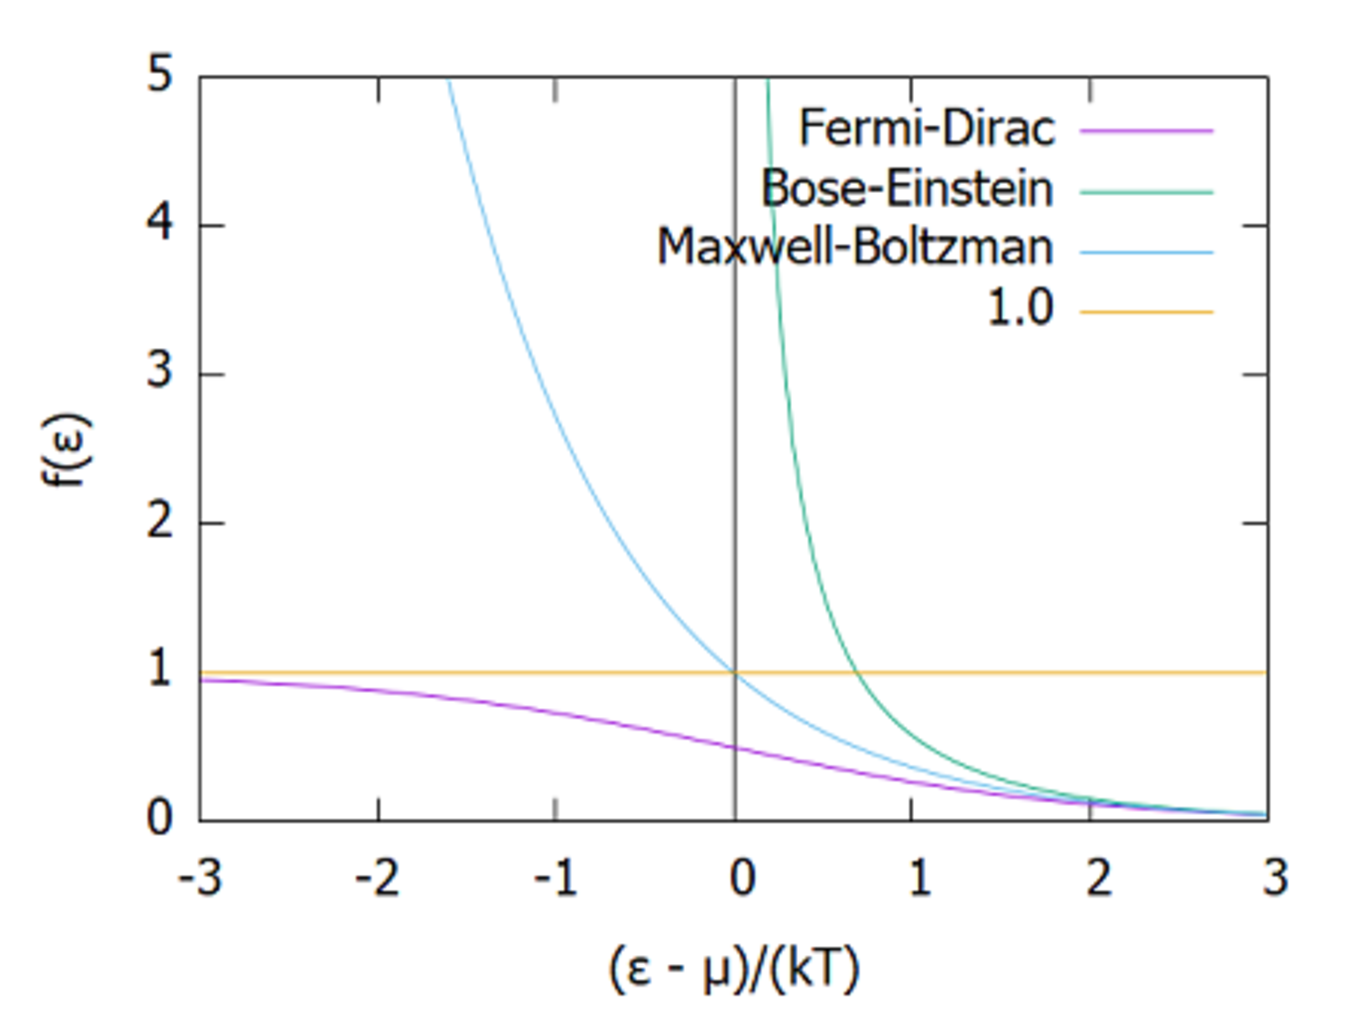
\includegraphics[width=14cm]{dist.eps}
			\caption{
			それぞれ、緑線:ボース・アインシュタイン分布、
			青線:マクスウェル・ボルツマン分布、
			紫線:フェルミ・ディラック分布を示す。
            		ボース・アインシュタイン分布では、励起状態の全粒子数がNより少ない場合、
            		残りの粒子は基底状態でなければならず、その占有数はいくらでも大きくなり、
            		ボース・アインシュタイン凝縮する。
            		また、$(\epsilon - \mu)/{\kb T}>>1$でそれぞれの分布が同じような傾向になり、
            		量子的な特徴が無くなっていく。これを古典領域という。
			}
			\label{FIG:bose}
		\end{figure}
		ボース・アインシュタイン分布の特徴は$(\epsilon - \mu) / (\kb T)$の下限では、非負で無限大となり、
        	上限ではマクスウェル・ボルツマン分布に漸近し量子性が失われる。
        	ボース粒子によるボースアインシュタイン凝縮と、フェルミ粒子によるフェルミ縮退の特徴の違いが
        	分布関数からも読み取ることができる~\cite{Pauli}。

        	つぎにボース・アインシュタイン凝縮相へ相転移となる条件の位相空間密度に着目する。
        	量子状態$l=k$における運動量空間$p(k)$のボース・アインシュタイン分布の平均は~(\ref{eq:becdist})から
        	\begin{eqnarray}
		    \langle n_k \rangle = \frac{1}{e^{\frac{\epsilon_k - \mu}{\kb T}} - 1},
        	\end{eqnarray}
        	とあらわされる。
        	粒子の質量を$m$、運動エネルギーを
        	\begin{eqnarray}
		    \epsilon_k = \frac{\hbar^2 k^2}{2 m},
        	\end{eqnarray}
        	とあらわし
        	各運動量空間の平均粒子数$\langle n_k \rangle$の総数を$N$とすると、
        	波数$k=0$の運動量空間とそれ以外に分けて以下のように示すことができる。
		\begin{eqnarray}
			N & = & \sum_k \langle n_k \rangle, \nonumber
			\\
			& = & \langle n_0 \rangle  + \frac{V}{(2\pi)^3} \int_0^\infty 4 \pi k^2 
			\langle n_k \rangle \diff k, \nonumber
			\\
			& = & \langle n_0 \rangle + \left( \frac{L}{2\pi} \right)^3 \int_0^\infty 4 \pi k^2
			\frac{1}{e^{\frac{\epsilon_k - \mu}{\kb T}} - 1} \diff k, \nonumber
			\\
			& = & N_0(T) + N^\prime(T),
		\end{eqnarray}
		$\langle n_0 \rangle$は基底状態の平均粒子数である。
		上記のように$N_0(T)$の基底状態の総粒子数、
        	励起状態の総粒子数を$N^\prime(T)$とすると、
		\begin{eqnarray}
			N^\prime(T) & = & \left(\frac{L}{2 \pi}\right)^3 \int_0^\infty 4 \pi k^2
			 \frac{1}{e^{\frac{\epsilon_k - \mu}{\kb T}} - 1}  \diff k,
		\end{eqnarray}
        	とあらわすことができ、これが最大となる条件を
		\begin{eqnarray}
			N^\prime_{{\rm max}}(T) & \ge & \left(\frac{L}{2 \pi}\right)^3 \int_0^\infty 4 \pi k^2
			 \frac{1}{e^{\frac{\hbar^2 k^2}{2 m} \cdot \frac{1}{\kb T}} - 1}  \diff k,
		\end{eqnarray}
        	とすれば、
		積分を$u = \frac{\hbar^2 k^2}{2 m \kb T}$で置換し$\Gamma$関数、$\zeta$関数を用いて、
        	$1/L^3$の密度の単位で書くと、
		\begin{eqnarray}
			\frac{N^\prime_{{\rm max}}(T)}{L^3} = n  & \ge & \left(\frac{1}{2 \pi} \right)^3 \cdot
			4 \pi \cdot \frac{m \kb T}{\hbar^2} \cdot \frac{\sqrt{2 m \kb T}}{\hbar} \cdot
			\int_0^\infty \frac{u^{1/2}}{e^u - 1} \diff u,
			\\
			& \ge & 4 \pi \cdot \frac{m \kb T}{h^2} \cdot \frac{\sqrt{2 m \kb T}}{h}
			\cdot \Gamma \left( 1+\frac{1}{2}\right) \zeta \left( 1+\frac{1}{2}\right), \nonumber
			\\
			& \ge & 4 \pi \cdot \frac{m \kb T}{h^2} \cdot \frac{\sqrt{2 m \kb T}}{h}
			\cdot \frac{\sqrt{\pi}}{2}\cdot \zeta \left( 1+\frac{1}{2}\right), \nonumber
			\\
			n & \ge & \left( \frac{\sqrt{2 \pi m \kb T}}{h} \right)^{3} \cdot 2.612,
		\end{eqnarray}
        	となる。
        	熱的ド・ブロイ波長を${\lambda_{{\rm dB}}} \equiv \frac{h}{\sqrt{2 \pi m \kb T}}$、
        	位相空間密度$\rho_{{\rm ps}} \equiv n \lambda_{{\rm dB}}^3$を定義すると、
		\begin{eqnarray}
            	\label{eq:thdlen}
			\rho_{{\rm ps}} = n \lambda_{{\rm dB}}^3 & \ge & 2.612,
		\end{eqnarray}
        	が得られ、理論上のボース・アインシュタイン凝縮へ相転移する条件を示している。


		\section{熱的ド・ブロイ波長とボース・アインシュタイン凝縮}
		~(\ref{eq:thdlen})とド・ブロイの物質波の関係式$p=\hbar/\lambda$から
		縮退温度、
		\begin{eqnarray}
            	\label{eq:temp}
			T(n) = \frac{2 \pi \hbar^2}{m k_{\rm B}}n^{2/3} < T_0,
		\end{eqnarray}
		が得られる。~(\ref{eq:temp})のグラフを図.~\ref{FIG:debroglie}に示す。
        	粒子数密度$n$に対し縮退温度以下$T(n)<T_0$の条件で量子的な効果が現れ、
		逆に縮退温度以上$T(n)>T_0$では、熱的ド・ブロイ波長よりも粒子の平均間隔が長くなり、
		物質波が現れず古典的な状態となる。
		\begin{figure}[H]
			\begin{center}
				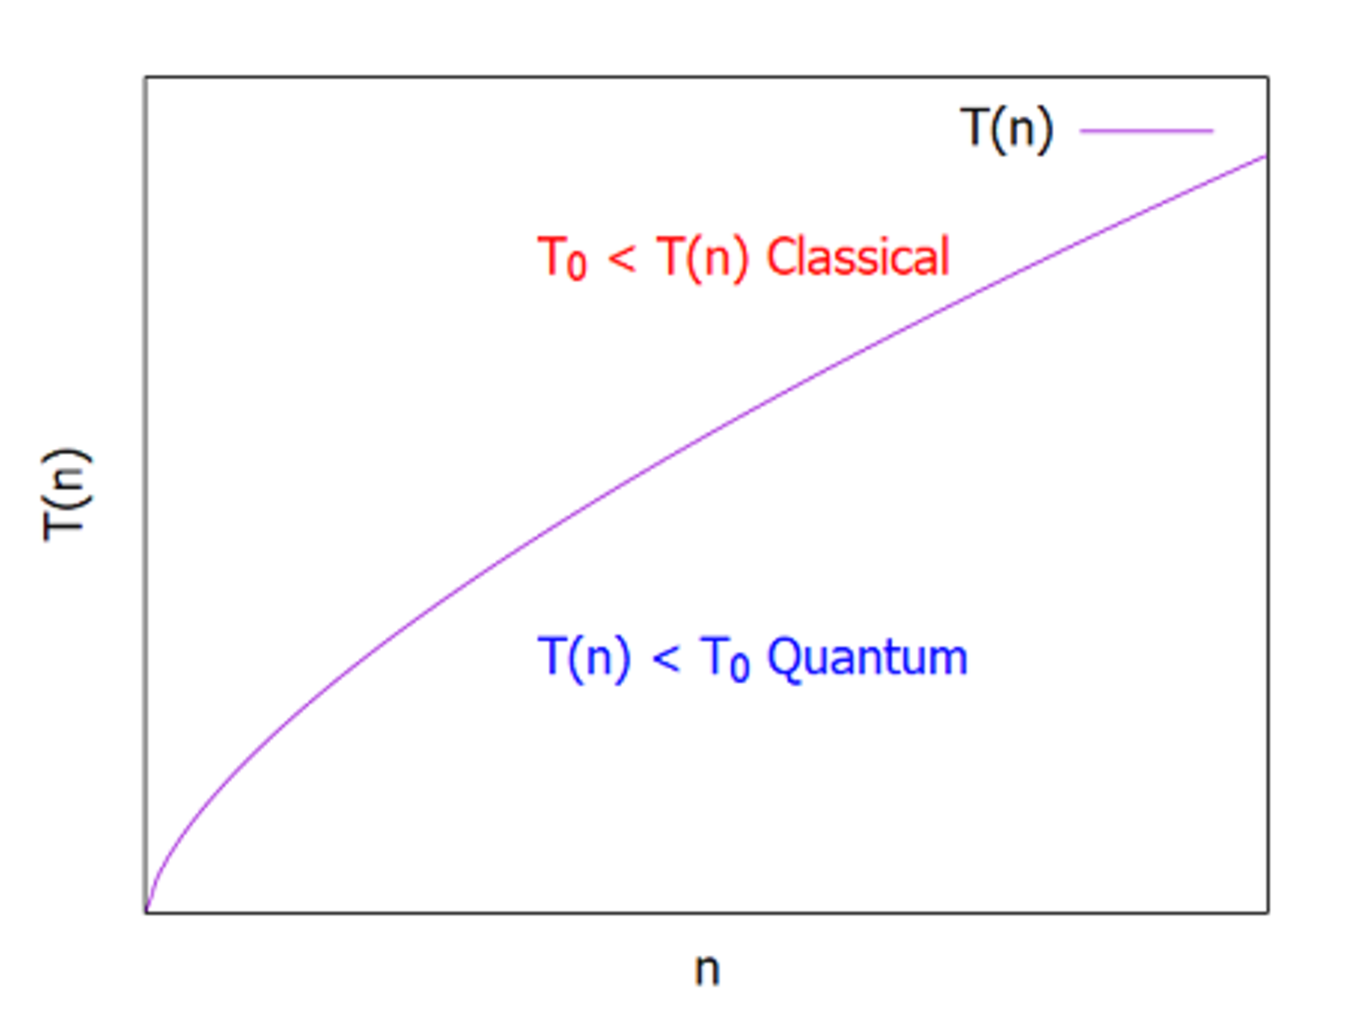
\includegraphics[width=14cm]{debroglie.eps}
				\caption{
                    縮退温度は粒子数密度$n$の$2/3$乗に比例する。
					縮退温度$T_0$以下では、位相空間密度が高くなり
                    波の性質が顕著な量子性の範囲となる。
				}
				\label{FIG:debroglie}
			\end{center}
		\end{figure}
        	熱的ド・ブロイ波長$\lambda_{{\rm dB}}$は
        	ボース・アインシュタイン凝縮の相転移で鍵となる物理量である。
        	室温では$\lambda_{{\rm dB}}$は原子サイズよりも小さいため古典力学的な粒子の運動が顕著にあらわれるが、
        	それとは対照に温度が下がるにつれ$\lambda_{{\rm dB}}$は大きくなり波の性質があらわとなる。
        	隣り合う原子と重なりあうと、全粒子として同じ位相の波をもつ単一の運動量状態になるため、
        	巨視的な波動関数が構成される~\cite{Pethick}。
		\begin{figure}[H]
			\begin{center}
				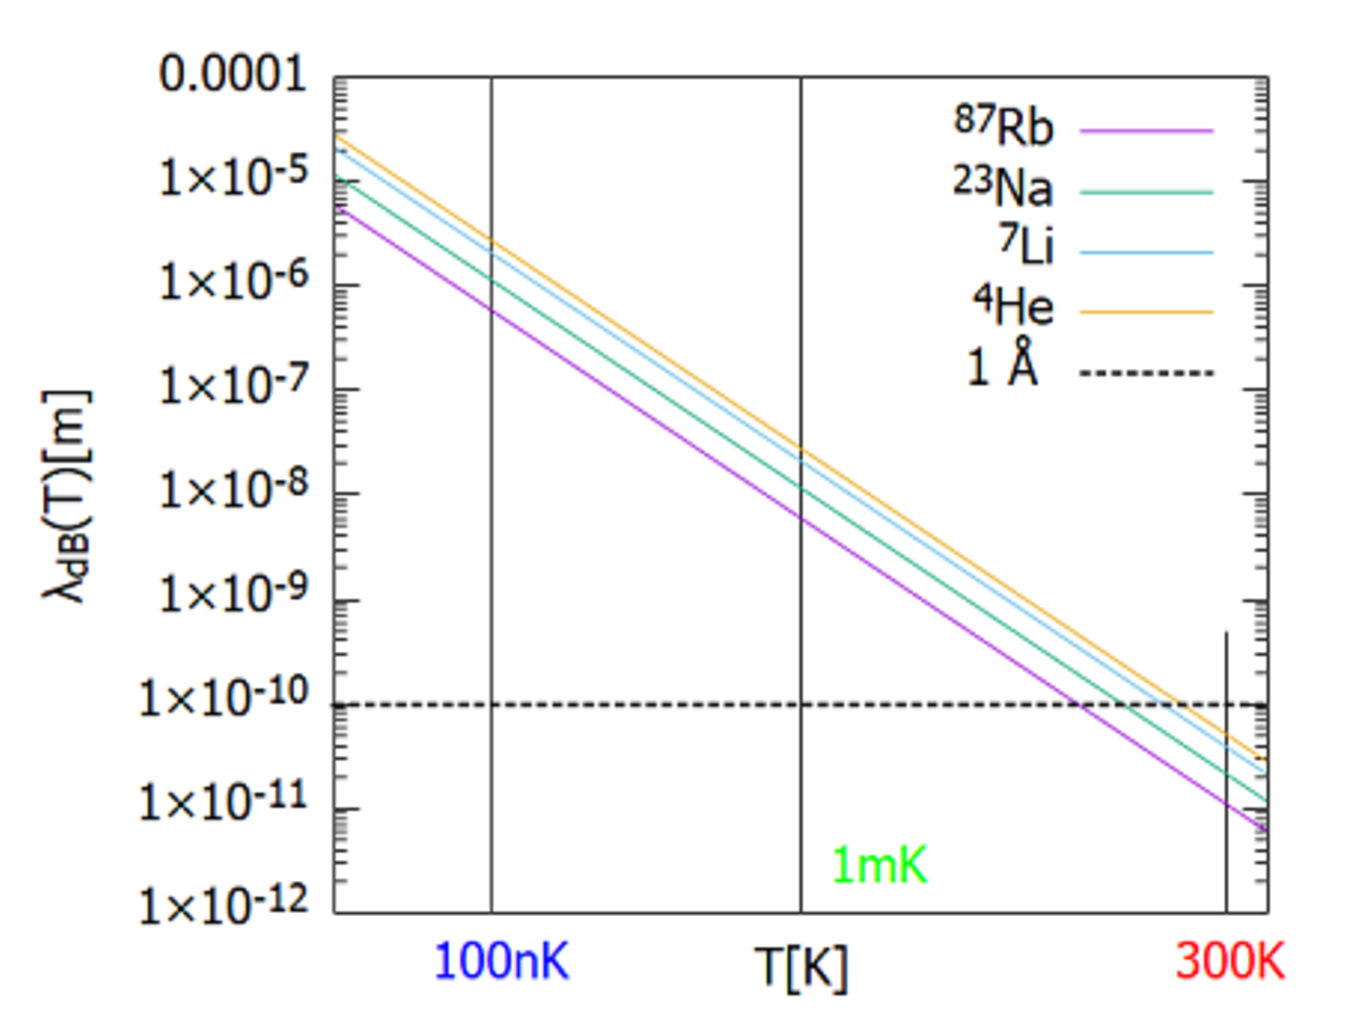
\includegraphics[width=14cm]{tlambda.eps}
				\caption{
					室温$(300{\rm K})$ではド・ブロイ波長$\lambda_{{\rm dB}}$は原子サイズよりも小さいが、
					縮退温度以下の領域では原子サイズよりもド・ブロイ波長は大きく広がる。
                    $^{87}{\rm Rb}$原子の直径はおよそ$0.5{\rm nm}$、$^{4}{\rm He}$原子の直径はおよそ$0.3{\rm nm}$。
				}
				\label{FIG:tlambda}
			\end{center}
		\end{figure}
		%$^{87}{\rm Rb}$の例で示すとおり、冷却により凝縮の臨界温度以下で粒子の持つ波長が原子直径よりも大きくなり、
		図.~\ref{FIG:tlambda}のグラフから、冷却により縮退温度以下で粒子の持つ波長が原子直径よりも大きくなることがわかる。
        	波長が大きくなるとエネルギーが低い基底状態に近づくにつれて原子集団は凝縮し、時間的空間的に位相が揃ったコヒーレント状態になる。
		ボース・アインシュタイン凝縮により量子力学的な特徴を持ちながら巨視的な状態に相転移する~\cite{Durfee}。
        	図.~\ref{FIG:bec}はその凝縮過程のイメージを示す。
		1995年のアンダーソンの実験では冷却温度$20{\rm nK}$で$^{87}{\rm Rb}$の
        	ボース・アインシュタイン凝縮の結果が得られている~\cite{Anderson}。
		\begin{figure}[H]
			\begin{center}
				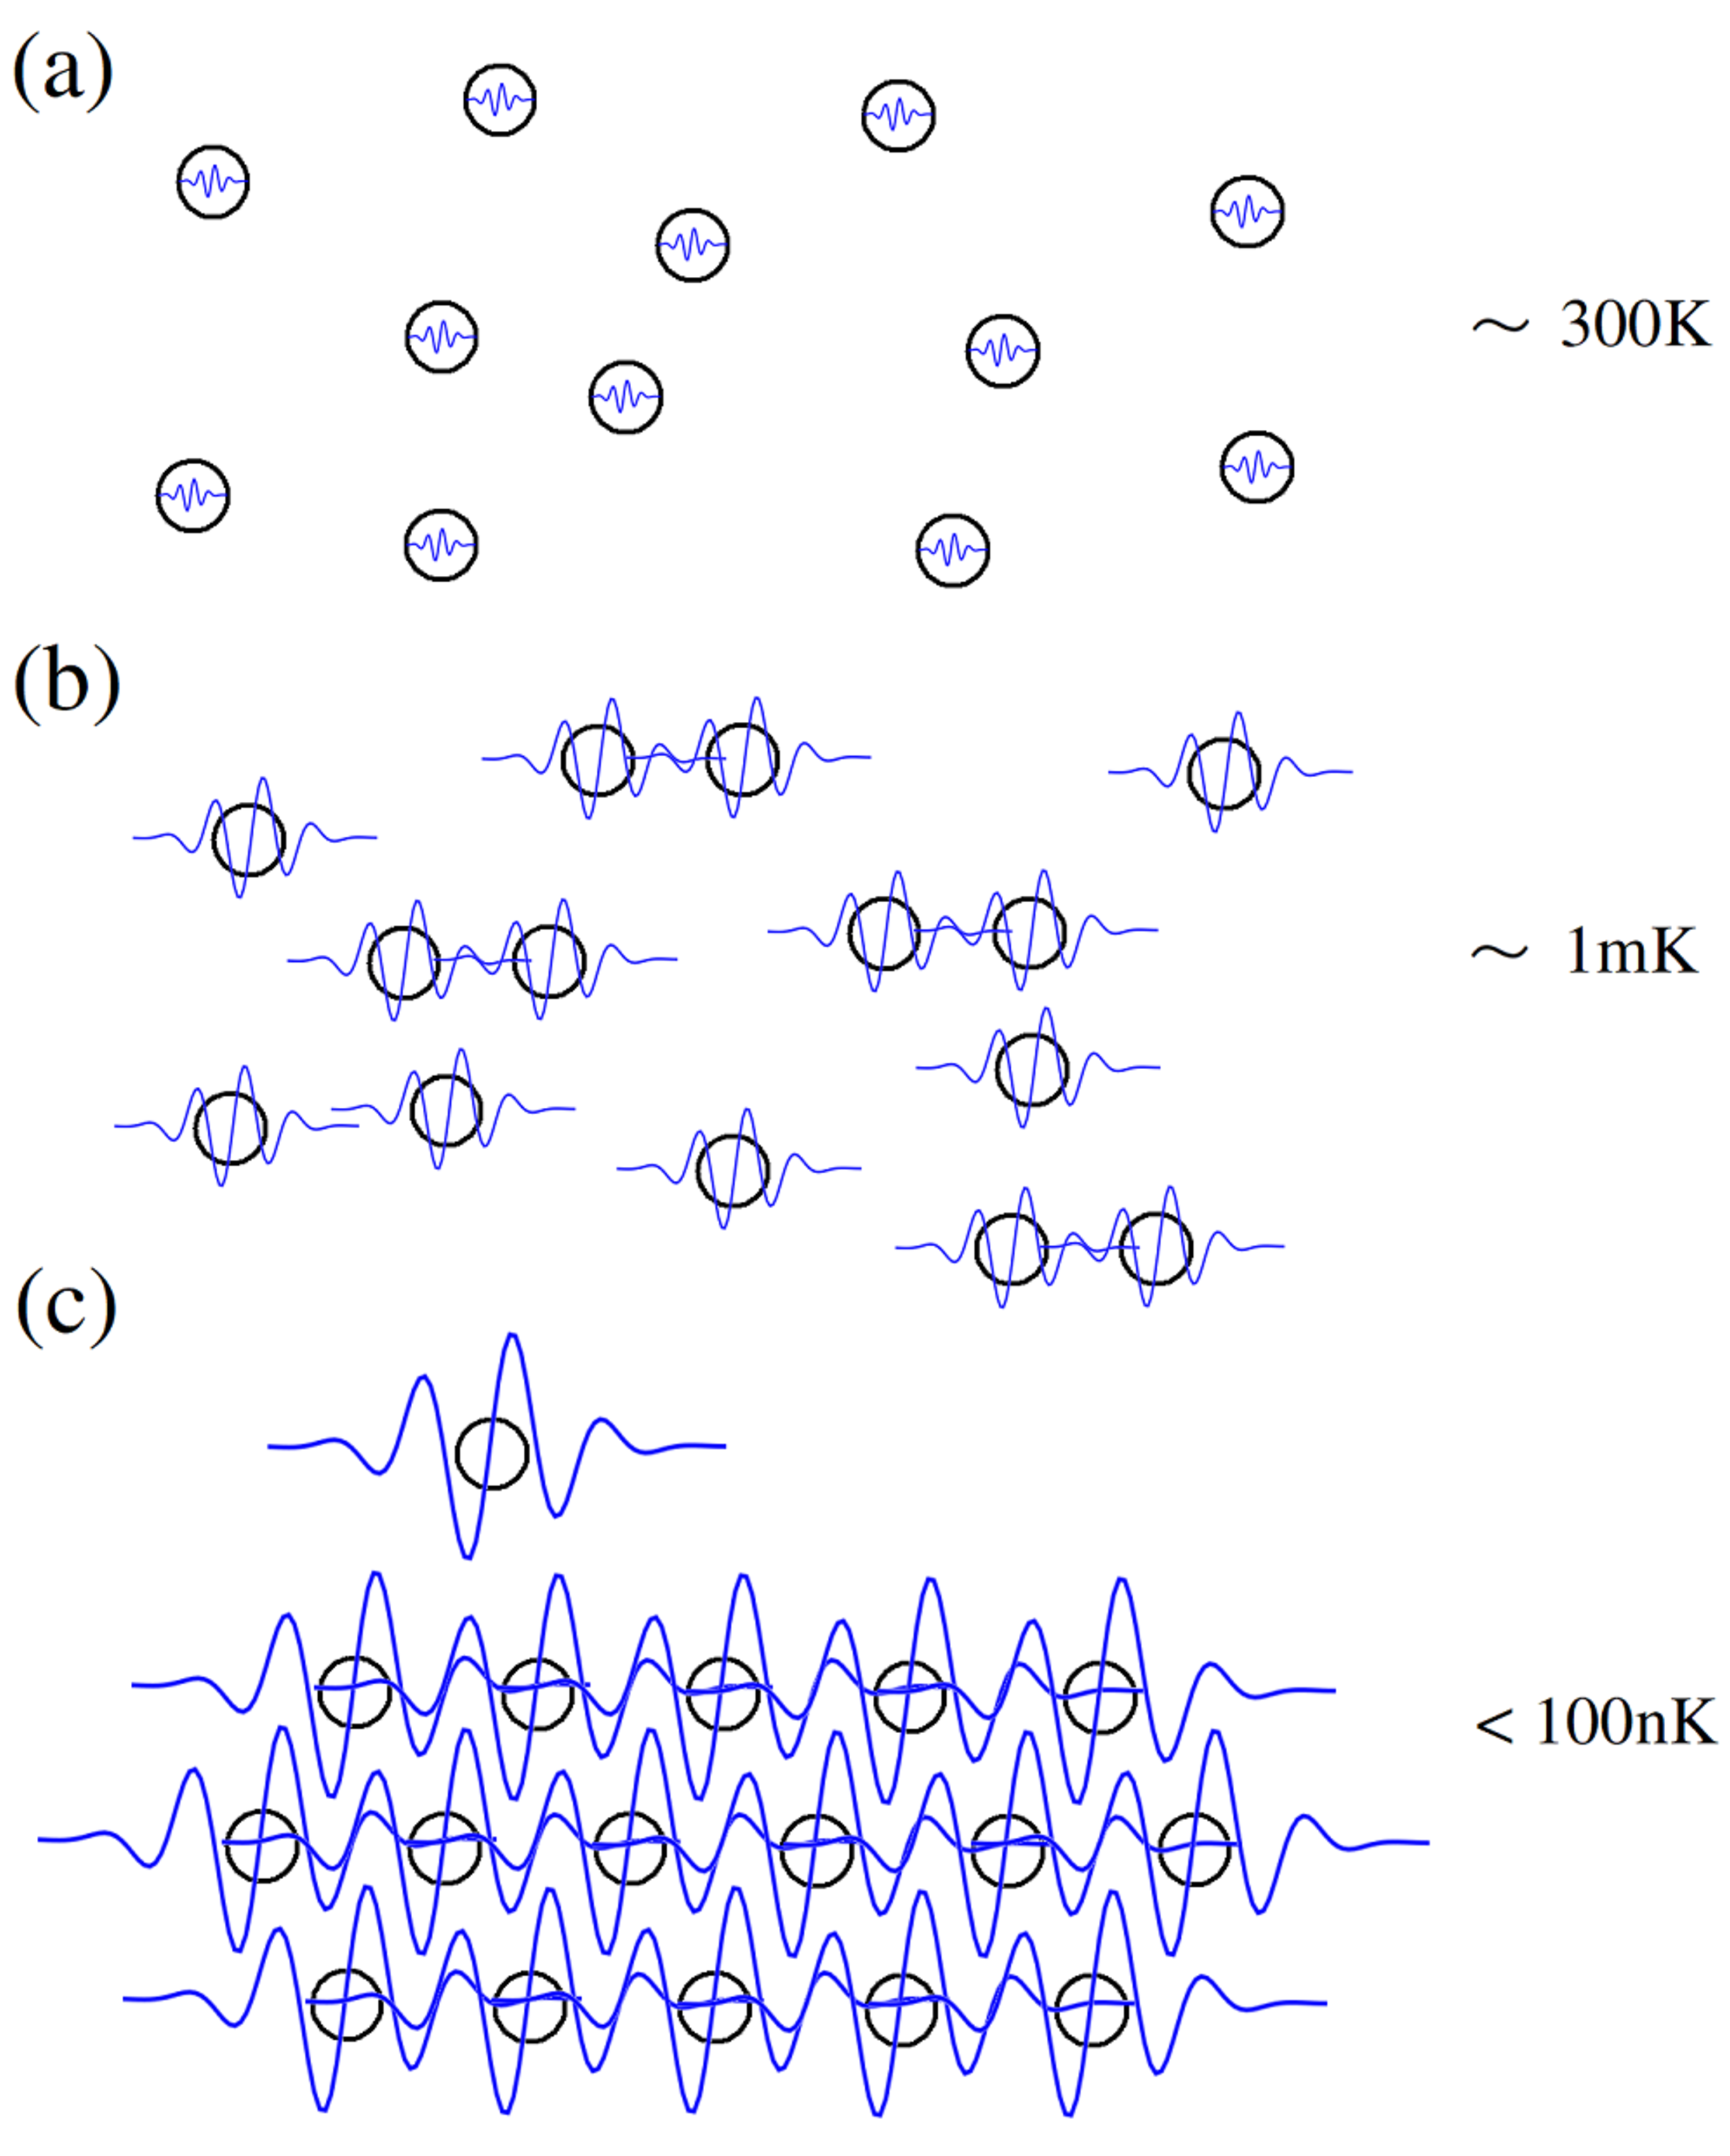
\includegraphics[width=11.5cm]{bec.eps}
				\caption{
                    黒丸は原子、青色の波束は熱的ド・ブロイ波長のイメージを示す。
                    $(a)$室温$(300{\rm K})$では熱的ド・ブロイ波長は原子サイズよりも小さく量子的な作用は現れない。
                    $(b)$冷却により、およそ$1{\rm mK}$ではしだいに波長が原子サイズから延び出す。
                    一部は近傍の原子とクラスターを生成し始める。
                    $(c)$およそ$100{\rm nK}$以下に達し、縮退温度に近づくと波の位相が時間的空間的に揃っていき、
                    原子集団が巨視的な量子状態となりボース・アインシュタイン凝縮する。
				}
				\label{FIG:bec}
			\end{center}
		\end{figure}

		%\section{BECの相転移温度}
		%冷却によりエネルギー最小の極限に達し、ボース・アインシュタイン凝縮した状況下の、
		%エネルギー固有値を考察する。
        	%一辺$L$の体積$L^3$における質量$m$、粒子数$N$の運動エネルギーの固有値は
		%\ The BEC is a phenomenon, in which all particles fall in the minimum energy state.
		%We consider the case in which $N$ atoms with mass $m$ are contained with a volume $L^3$.
		%The eigenvalue $\epsilon_k$ of the kinetic energy is given by
		%\begin{eqnarray}
		%	\epsilon_k = \frac{\hbar^2 k^2}{2m} = \frac{\hbar^2}{2m}(k_x^2+k_y^2+k_z^2).
		%\end{eqnarray}
        	%で与えられる。
        	%波数ベクトルは、
		%\begin{eqnarray}
		%	(k_x, k_y, k_z) & = & \frac{2 \pi}{L}(n_x, n_y, n_z),
		%\end{eqnarray}
		%where $n_x,n_y,n_z = 0, 1, 2, \cdots$ .
		%Subtracting the number of atoms in the ground state $N_0$ from
		%the total number of atoms $N$,
		%we have the number of excited atoms as
		%\begin{eqnarray}
	    	%	N - N_0 = \sum_{k \neq 0} \frac{1}{ e^{\beta (\epsilon_k - \mu)} - 1},
		%\end{eqnarray}
		%%where $\beta = 1/(\kb T)$.
		%Replacing the summation with an integral approximation for a large system as
		%\begin{eqnarray}
		%	\frac{1}{V} \sum_{k \neq 0} & \rightarrow & \int \frac{\diff^3 k}{(2 \pi)^3}.
		%\end{eqnarray}
		%At temperature $T$, expectation value of the number atoms in $k$ state
		%with an energy $\epsilon_k$ is calculated as
		%\begin{eqnarray}
		%	\langle n_k \rangle & = & \frac{1}{e^{\frac{\epsilon_k - \mu}{\kb T}} - 1},
		%\end{eqnarray}
        	%%where $\mu \leq 0$. The chemical potential $\mu$ is determined in
		%such a way that $N = \sum_k \langle n_k \rangle$.
		%The total number of atoms then becomes
        	%粒子の総数、
		%\begin{eqnarray}
		%	N & = & \sum_k \frac{1}{e^{\frac{\epsilon_k - \mu}{\kb T}} - 1}.
		%\end{eqnarray}
		%We replace the summation with the integration using the density of state,
		%\begin{eqnarray}
		%	N & = & \int_{-\infty}^{\infty} \frac{ D(\epsilon)}{e^{\frac{\epsilon_k - \mu}{\kb T}} - 1}
		%	\diff \epsilon.
		%\end{eqnarray}
		%We define the density of states
		%\begin{eqnarray}
		%	D(\epsilon) & = & 2 \pi V \left( \frac{2m}{\hbar^2} \right)^{\frac{3}{2}} \sqrt{\epsilon}.
		%\end{eqnarray}
        	%熱的ド・ブロイ波長で書きあらわし、
		%\begin{eqnarray}
		%	\lambda_{\rm d} & = & \frac{\hbar}{\sqrt{2 \pi m \kb T}},
		%\end{eqnarray}
		%Equation (2.30) is shown to be
		%\begin{eqnarray}
		%	N - N_0 & = & \frac{V}{\lambda_{\rm d}^3} b_{3/2} (z).
		%\end{eqnarray}
		%Where the function $b_{n}(z)$ is the Bose-Einstein integration,
		%\begin{eqnarray}
		%	b_n (z) & = & \frac{1}{\Gamma (n)} \int_0^\infty \frac{x^{n-1}}{e^{\frac{x}{z}}-1} \diff x.
		%\end{eqnarray}
		%At high temperature, the right-hand side of Eq.(2.37) is of order of N.
		%However at low temperature,
		%$N_0$ is much smaller than $N$.
		%Then, Eq.(2.37) with $N_0 = 0, \mu = 0$ becomes as
		%\begin{eqnarray}
		%	b_{\frac{3}{2}}(z) \leq b_{\frac{3}{2}}(1) = \zeta \left( \frac{3}{2} \right) = 2.6128 \cdots.
		%\end{eqnarray}
        	%極低温の環境下では、
		%At low temperature, in the right-hand side of Eq.(2.37),
		%the number of atoms in the ground state, $N_0$ becomes dominant T, giving
		%\begin{eqnarray}
		%	N & = & \frac{V}{\lambda_{\rm d}^3 b_{\frac{3}{2}} }(1).
		%\end{eqnarray}
        	%となり、ボース・アインシュタイン凝縮となる臨界温度$T_c$
		%\begin{eqnarray}
		%	T_c & = &
		%	\left[ \zeta \left( \frac{3}{2} \right) \right]^{-\frac{2}{3}} \frac{2 \pi \hbar^2}{m \kb}
		%	\left( \frac{N}{V} \right)^{\frac{2}{3}},
		%\end{eqnarray}
        	%が得られる。


		\section{非対角長距離秩序}
        	ボース・アインシュタイン凝縮の状態下では、ボース粒子が巨視的な数の集団で構成し
        	波の反射や干渉、音速など波動性のある超流動体として知られている。
        	超流動の流体秩序は非対角長距離秩序によってあらわされる。
        	ここでは本研究で取り扱うボース粒子の非対角長距離秩序について概説する。
        	体積$V$の空間にある運動量$k=l$の状態のボース粒子の
        	場について、フーリエ変換が可能な場の演算子$\hat{\psi}^\dagger(\Vec{r}),\hat{\psi}(\Vec{r})$を
        	生成演算子$\hat{a}^\dagger_{\Vec{k}}$と消滅演算子$\hat{a}_{\Vec{k}}$、
        	\begin{eqnarray}
            		\left[ \hat{a}^\dagger_{\Vec{k}}, \hat{a}_{\Vec{k}^\prime} \right] & = & 
            		\delta_{\Vec{k},\Vec{k}^\prime},
            		\\
            		\left[ \hat{a}^\dagger_{\Vec{k}}, \hat{a}^\dagger_{\Vec{k}^\prime} \right] & = & 
            		\left[ \hat{a}_{\Vec{k}}, \hat{a}_{\Vec{k}^\prime} \right] = 0,
        	\end{eqnarray}
        	を用いて、
        \begin{eqnarray}
            \label{qe:cre_ann}
            \hat{\psi}^\dagger(\Vec{r}) & = & \frac{1}{\sqrt{V}} \sum_{\Vec{k}} \hat{a}^\dagger_{\Vec{k}} e^{-i \Vec{k} \cdot \Vec{r}},
            \\
            \hat{\psi}(\Vec{r}) & = & \frac{1}{\sqrt{V}} \sum_{\Vec{k}} \hat{a}_{\Vec{k}} e^{i \Vec{k} \cdot \Vec{r}},
        \end{eqnarray}
        とあらわす。$\delta_{\Vec{k},\Vec{k}^\prime}$はデルタ関数を示す。長さ$L$の体積$V=L^3$の空間で
        規格化条件$\int d^3 \Vec{r} | \psi(\Vec{r})|^2 = 1$から$\frac{1}{\sqrt{V}}$で規格化する。
        波数$\Vec{k}=(k_x, k_y, k_z)$は、
        \begin{eqnarray}
            (k_x, k_y, k_z) = \left(
                \frac{2 \pi}{L}n_x, \frac{2 \pi}{L}n_y, \frac{2 \pi}{L}n_z
            \right)
            \ , \
            (n_x, n_y, n_z : 整数),
        \end{eqnarray}
        の周期的境界条件を課す。波数の和は
        \begin{eqnarray}
            \sum_{\Vec{k}} \left[ \cdots \right] 
            = \sum^{\infty}_{n_x = -\infty} \sum^{\infty}_{n_y = -\infty} \sum^{\infty}_{n_z = -\infty} \left[ \cdots \right],
        \end{eqnarray}
        であらわし、$L \rightarrow \infty$の極限で
        \begin{eqnarray}
            \sum_{\Vec{k}} \left[ \cdots \right] \equiv \int \frac{d \Vec{k}^3}{(2\pi)^3} \left[ \cdots \right],
        \end{eqnarray}
        を定義する。
        波動関数$\hat{\psi}^\dagger(\Vec{r}),\hat{\psi}(\Vec{r})$
        から以下の密度行列は、数密度演算子
        $
            \hat{n}_{\Vec{k}} =\hat{a}^\dagger_{\Vec{k}} \hat{a}_{\Vec{k}}
        $
        を用いて、
        \begin{eqnarray}
            \rho(\Vec{r},\Vec{r}^\prime) & = & \langle \hat{\psi}^\dagger(\Vec{r}) \hat{\psi}(\Vec{r}^\prime) \rangle,
            \\
            & = & \frac{1}{V}\sum_{\Vec{k}} \langle
                \hat{a}^\dagger_{\Vec{k}} \hat{a}_{\Vec{k}}  
            \rangle
            e^{-i \Vec{k} \cdot (\Vec{r} - \Vec{r}^\prime)},
            \\
            \label{eq:denmx}
            & = & \frac{\langle \hat{n}_0 \rangle}{V} + \frac{1}{V}\int \frac{d\Vec{k}^3}{(2\pi)^3} \langle \hat{n}_{\Vec{k}} \rangle 
            e^{- i \Vec{k} \cdot (\Vec{r}-\Vec{r}^\prime)}
            = \rho(\Vec{r}-\Vec{r}^\prime),
        \end{eqnarray}
        が得られ、$\Vec{k}=0$の基底状態とそれ以外の励起状態であらわす。
        非対角の長距離$|\Vec{r}-\Vec{r}^\prime|\rightarrow \infty$では、励起状態の~(\ref{eq:denmx})の第$2$項が
        フーリエ級数展開した三角関数の重ね合わせであるため、
        リーマン・ルベーグの定理により高次のフーリエ係数が収束し$0$に漸近する。
        %励起状態は無秩序相といえる。
        結果として秩序相となる基底状態の第$1$項、
        \begin{eqnarray}
            \lim_{|\Vec{r}-\Vec{r}^\prime|\rightarrow \infty} \rho(\Vec{r}-\Vec{r}^\prime) = \frac{\langle \hat{n}_0 \rangle}{V},
        \end{eqnarray}
        が残る。
        任意の空間$\Vec{r}-\Vec{r}^\prime$では、
        \begin{eqnarray}
            \rho(\Vec{r}-\Vec{r}^\prime)V = n_0 \neq 0,
        \end{eqnarray}
        となり非対角成分が有限の値で残る。
        図.~\ref{FIG:odlro}で示すように極低温の環境下では基底状態の系が数密度$n_0$で巨視的に広がる。
        これをボース・アインシュタイン凝縮における非対角長距離秩序という。
        極低温ではない縮退温度以上$T>T_{\rm c}$の環境下の古典領域では、
        基底状態の系$\frac{\langle \hat{n}_0 \rangle}{V}$が無いために数密度$n_0$は存在しない。
		\begin{figure}[H]
			\begin{center}
				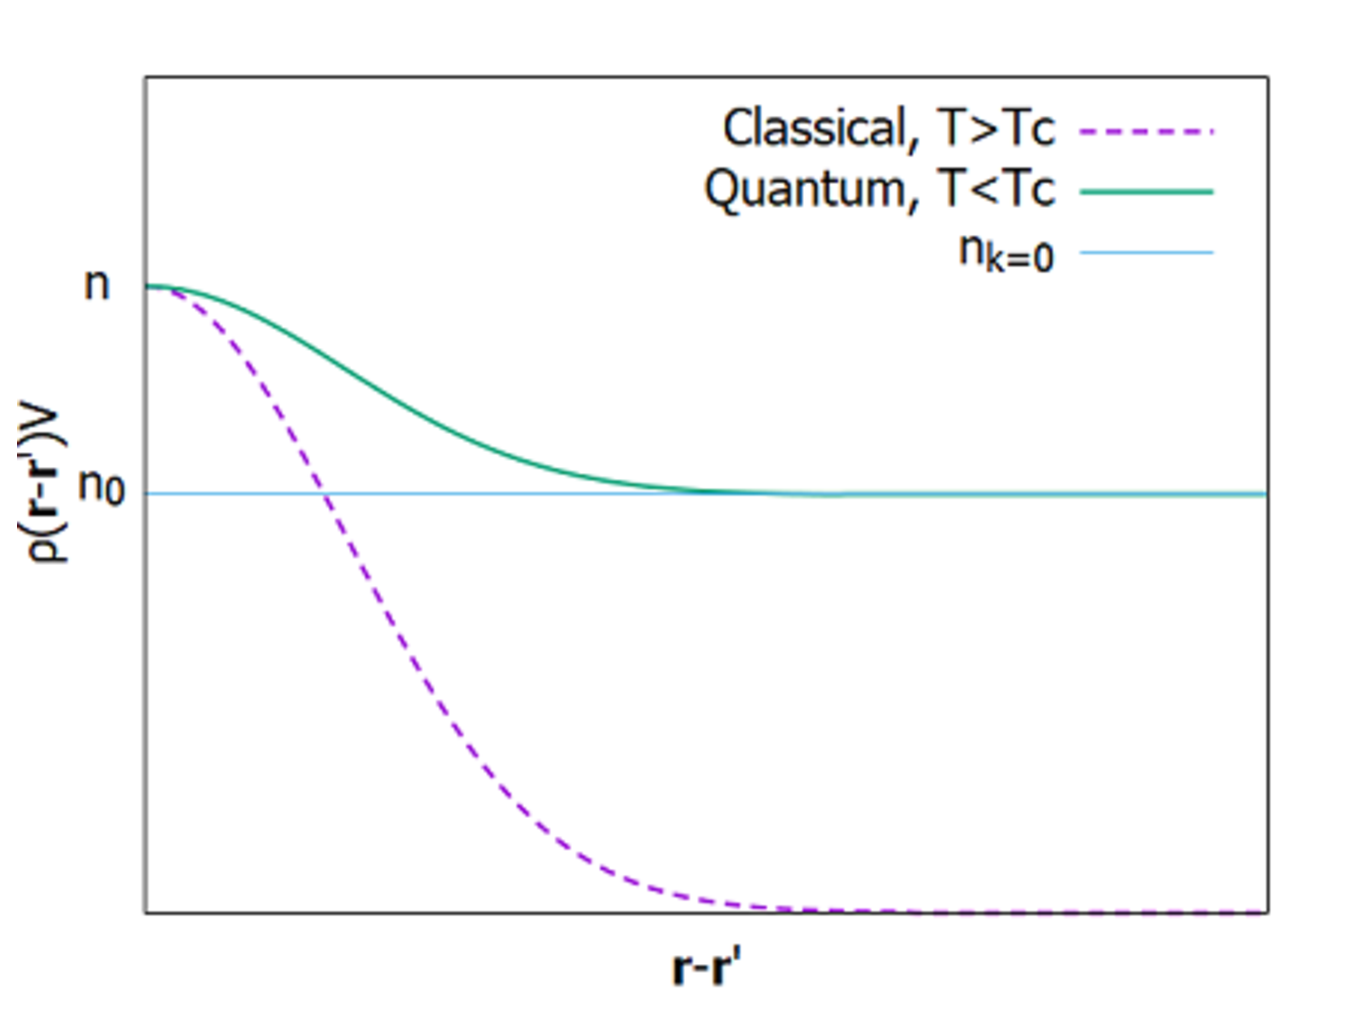
\includegraphics[width=14cm]{odlro.eps}
				\caption{
					$t<T_c$で、波数$k=0$の状態にボース・アインシュタイン凝縮すると
					全粒子数$N$の増加に比例して、$k=0$の平均数密度$\langle \hat{n_o} \rangle$も増えるため
					長距離相関で有限の値$n_0 \neq 0$となる。
                    \\
					$T>T_c$では秩序相となる$k=0$の基底状態の粒子がなく、
                    無秩序相の励起状態の量子のみであるため長距離相関で数密度$n$は$0$となる。
				}
				\label{FIG:odlro}
			\end{center}
		\end{figure}
		例として図.~\ref{FIG:odlro2}で、
		非対角長距離秩序が存在する超流動体の波の干渉を示す。
        数値計算は平均場近似を示すグロス・ピタエフスキー方程式
        を擬スペクトル法を用いて算出した。
        数値計算の詳細については~\ref{s:numeric}(A)で示す。
        $(x,y)=(\pm5,\pm5)$の二次元空間の系で、初期状態$(x,y)=(-2,0),(2,0)$の二ヶ所に、
        ピーク値$0.1$、半値全幅$2$のガウシアン分布で配置した
        超流動体を一定速度で$(x,y)=(0,0)$の位置へ移動させ衝突する様子である。
        $(a)$~$(d)$は二つの超流動体が
        衝突し波の干渉が生じる。$(a^\prime)$~$(d^\prime)$は同時刻の位相をあらわす。
		\begin{figure}[H]
			\begin{center}
				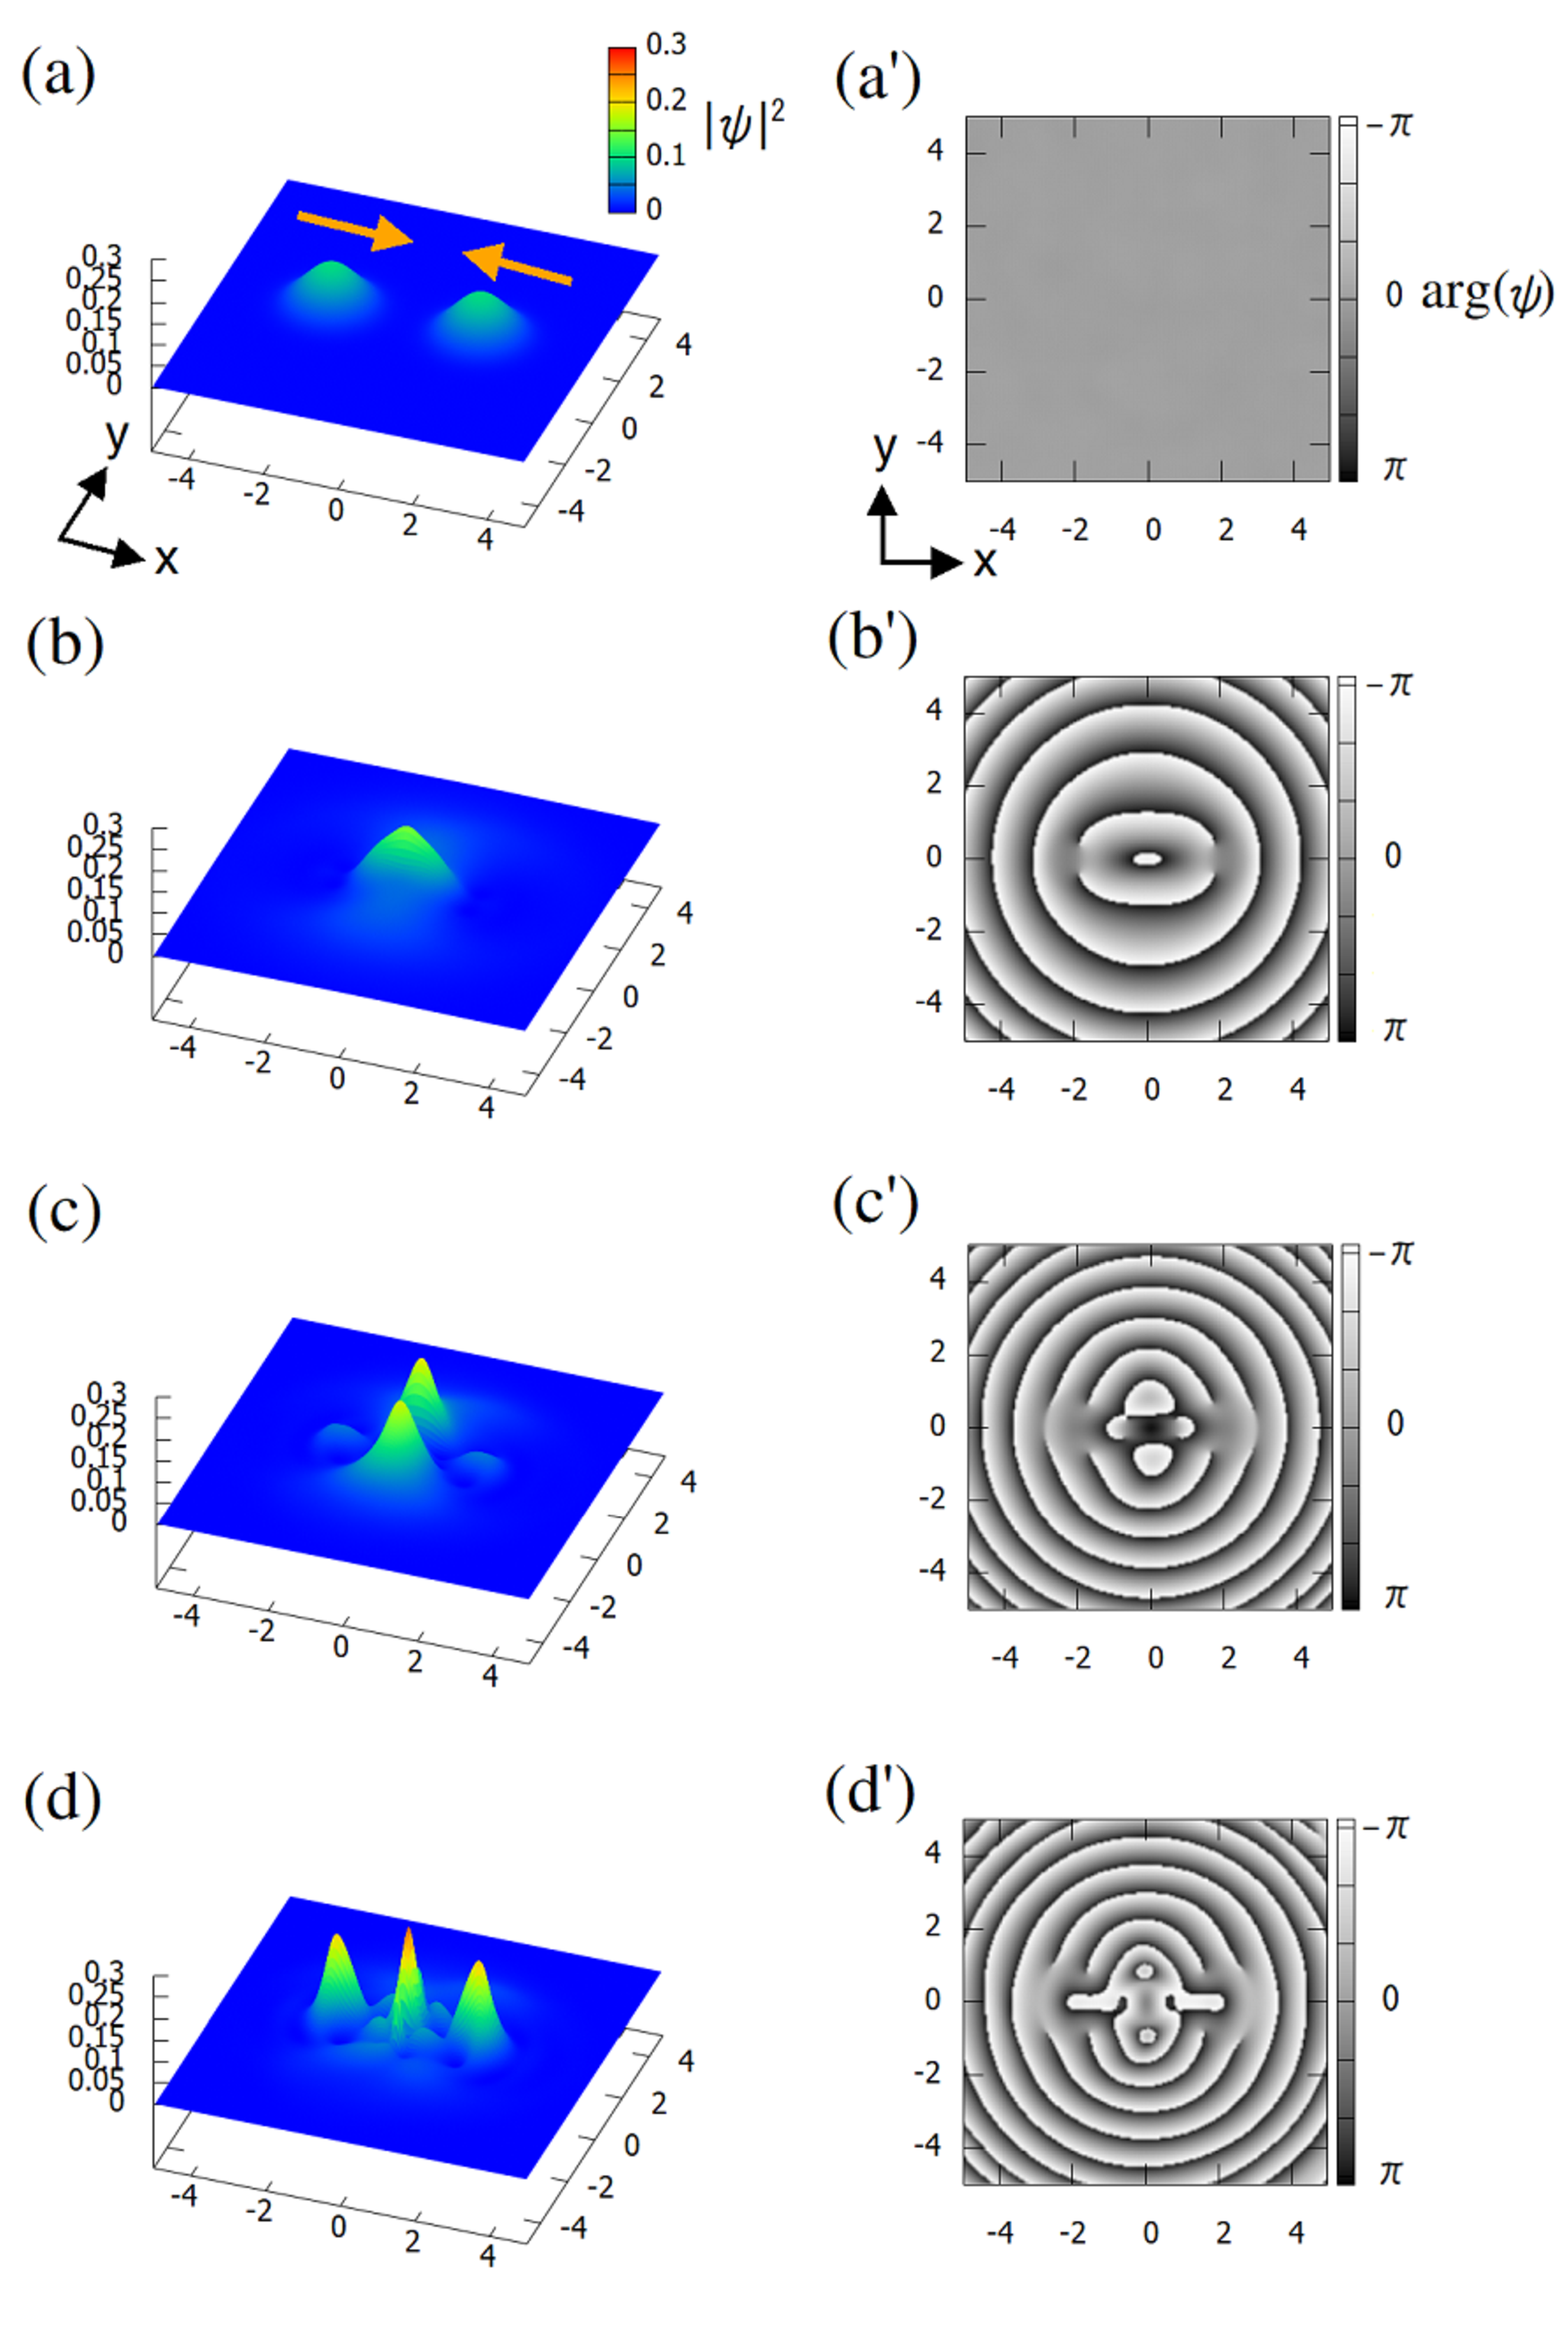
\includegraphics[width=14cm]{odlro2.eps}
				\caption{
					$(a)$~$(d)$の順に時間発展した確率密度、$(a^\prime)$~$(d^\prime)$は同時刻の位相を示す。
                    $(x,y)=(\pm5,\pm5)$の二次元空間の系で、初期状態$(x,y)=(-2,0),(2,0)$の二ヶ所に、
                    ピーク値$0.1$、半値全幅$2$のガウシアン分布で配置した
                    超流動体を一定速度で$(x,y)=(0,0)$の位置へ移動させ衝突する様子。
					巨視的な超流動体の系で波の干渉が現れる。
                    数値計算は擬スペクトル法を用いて算出した。
                    詳細については~\ref{s:numeric}(A)にて示す。
				}
				\label{FIG:odlro2}
			\end{center}
		\end{figure}


		\section{グロス・ピタエフスキー方程式による平均場近似}
        ポテンシャル$V_{\rm ext}(\Vec{r})$中にある粒子数$N=\sum_k n_k$のボース粒子の多体ハミルトニアンの
        平均場近似を考える。
        ポテンシャルによりトラップされたボース粒子のハミルトニアンは、
        \begin{eqnarray}
            \label{eq:fham}
            \hat{H} = \int d \Vec{r} \hat{\psi}^\dagger (\Vec{r}) \left[
                -\frac{\hbar^2}{2m} \Vec{\nabla}^2
                +V_{\rm ext}(\Vec{r})
            \right]
            \hat{\psi}(\Vec{r})
            + \int d \Vec{r}^\prime \hat{\psi}^\dagger(\Vec{r}) \hat{\psi}^\dagger(\Vec{r}^\prime)
            U(\Vec{r}-\Vec{r}^\prime)
            \hat{\psi}(\Vec{r}^\prime) \hat{\psi}(\Vec{r}),
        \end{eqnarray}
        であらわされる。
        $m$は粒子の質量、$\hat{\psi}(\Vec{r})$は場の演算子$\hat{\psi}(\Vec{r})=\sum_k \psi_k(\Vec{r})a_k$、
        $a_k$は生成消滅演算子$a_k|n_0, n_1, \cdots n_k \rangle=\sqrt{n_k}|n_0, n_1, \cdots n_k-1 \rangle,
        a^\dagger_k|n_0, n_1, \cdots n_k \rangle=\sqrt{n_k+1}|n_0, n_1, \cdots n_k+1 \rangle$である。
        $U(\Vec{r} - \Vec{r}^\prime)$は
        相互作用をあらわす擬ポテンシャル$U(\Vec{r} - \Vec{r}^\prime) = g \delta(\Vec{r} - \Vec{r}^\prime)$である。
        $g$は結合定数$g = \frac{4 \pi \hbar^2 a_s}{M}$、$a_s$はボース粒子の$S$波散乱長、$M$は有効質量を示す。
        場の演算子$\hat{\psi}(\Vec{r},t)$の時間発展について、ハミルトニアン~(\ref{eq:fham})を用いて
        ハイゼンベルク描像の運動方程式、
        \begin{eqnarray}
            \label{eq:fgpe}
            i \hbar \frac{\partial}{\partial t} \hat{\psi}(\Vec{r},t) 
            & = & \left[ \hat{\psi}(\Vec{r},t), \hat{H} \right], \nonumber
            \\
            & = & \left[
                - \frac{\hbar^2}{2m} + V_{\rm ext} (\Vec{r})
                + \int d \Vec{r}^\prime \hat{\psi}^\dagger (\Vec{r}^\prime,t)
                U(\Vec{r} - \Vec{r}^\prime) \hat{\psi}(\Vec{r}^\prime,t)
            \right] \hat{\psi}(\Vec{r},t), \nonumber
            \\
            & & 
        \end{eqnarray}
        を得る。
        演算子について$\hat{\psi}(\Vec{r},t)=\psi(\Vec{r},t)+\hat{\psi}^\prime (\Vec{r},t)$と古典場と
        それ以外の摂動に分ける。古典場は平均値$\psi(\Vec{r},t) \equiv \langle \hat{\psi}(\Vec{r},t) \rangle$で定義する。
        極低温下では、摂動を除く凝縮体となったボース粒子の数が支配的となり、~(\ref{eq:fgpe})を古典場の平均値で近似し、
		\begin{eqnarray}
            \label{eq:gpe}
			i \hbar \frac{\partial}{\partial t} \psi ( \Vec{r}, t ) & = &
            \left[
			-\frac{\hbar^2}{2m} \nabla^2
            + V_{\rm ext}(\Vec{r})
			+ g | \psi(\Vec{r}, t) |^2
            \right]\psi(\Vec{r},t),
		\end{eqnarray}
        となり、ボース・アインシュタイン凝縮体の運動を近似する
        グロス・ピタエフスキー(GP)方程式を得る~\cite{Pitaevskii2}。


        \section{回復長}
        GP方程式~(\ref{eq:gpe})の運動エネルギーの項と相互作用ポテンシャルの項の比から
        回復長(healing length)といわれる特徴的な長さの単位、
        \begin{eqnarray}
            \xi = \frac{\hbar}{\sqrt{2mgn_0}},
        \end{eqnarray}
        が得られ、数値計算の無次元化などに用いられる。
        $n_0$は凝縮体の数密度$n_0 \equiv |\psi|^2$で定義する。
        また、超流動体の運動エネルギーが斥力の相互作用ポテンシャルの大きさに達したときのサイズとして、
        \begin{eqnarray}
            \frac{\hbar^2}{2m \xi^2} \simeq g n_0,
        \end{eqnarray}
        があらわされる。


		\section{量子流体力学と量子渦}
		波数$k=0$に凝縮した超流動体の数密度$n_0=|\psi|^2$を秩序パラメータと見立てて、
		古典の流体力学と同等な連続の式とオイラー方程式が得られる。
        そこから展開される分野を量子流体力学という~\cite{quantumfluid}。
        簡単のため$\psi(\Vec{r},t)=\psi$と簡略し、
        GP方程式~(\ref{eq:gpe})とその複素共役
        \begin{eqnarray}
            \label{eq:ccgpe}
			-i \hbar \frac{\partial}{\partial t} \psi^\dagger & = &
            \left[
			-\frac{\hbar^2}{2m} \nabla^2
            + V_{\rm ext}(\Vec{r})
			+ g|\psi|^2
            \right]\psi^\dagger,
        \end{eqnarray}
        のそれぞれに、右から$\psi^\dagger$、$\psi$をかけて差をとる。
        \begin{eqnarray}
            i \hbar \frac{\partial \psi}{\partial t}\psi^\dagger
            - \left(
                -i \hbar \frac{\partial \psi^\dagger}{\partial t}\psi
            \right)
            & = &
            \left[ - \frac{\hbar^2}{2m} ( \Vec{\nabla}^2 \psi ) \psi^\dagger \right]
            - \left[ - \frac{\hbar^2}{2m} ( \Vec{\nabla}^2 \psi^\dagger ) \psi \right] \nonumber
            \\
            & & + V_{\rm ext}(\Vec{r}) \psi \psi^\dagger - V_{\rm ext}(\Vec{r}) \psi^\dagger \psi \nonumber
            \\
            & & + g|\psi|^2 \psi \psi^\dagger - g|\psi|^2 \psi^\dagger \psi, \nonumber
            \\
            i \hbar \frac{\partial |\psi|^2}{\partial t} & = & - \frac{\hbar^2}{2m} \Vec{\nabla} \cdot 
            \left(
                \psi^\dagger \Vec{\nabla} \psi - \psi \Vec{\nabla} \psi^\dagger
            \right),
        \end{eqnarray}
        ここで、速度場
        \begin{eqnarray}
            \label{eq:vfld}
            \Vec{v}(\Vec{r},t) \equiv \frac{\hbar}{2mi} \frac{\psi^\dagger \Vec{\nabla} \psi - \psi \Vec{\nabla} \psi^\dagger}{|\psi|^2},
        \end{eqnarray}
        を定義し、
        秩序パラメータを$\psi=\sqrt{n_0}e^{i \theta}$とすると、
        \begin{eqnarray}
            \label{eq:qcont}
            \frac{\partial n_0}{\partial t} + \Vec{\nabla} \cdot (n_0 \Vec{v}) = 0,
        \end{eqnarray}
        の連続の式が得られる。
        速度場~(\ref{eq:vfld})から、
        \begin{eqnarray}
            \psi^\dagger \Vec{\nabla} \psi - \psi \Vec{\nabla} \psi^\dagger
            & = & \left[ 
                \sqrt{n_0} e^{i \theta} + i \sqrt{n_0} (\Vec{\nabla} )e^{i \theta} 
            \right] \sqrt e^{i \theta}
            - \left[
                \sqrt{n_0} e^{-i \theta} - i \sqrt{n_0} ( \Vec{\nabla} )e^{-i \theta}
            \right] \sqrt e^{i \theta}, \nonumber
            \\
            & = & i 2 n_0 \Vec{\nabla} \theta,
        \end{eqnarray}
        の等式を用いて、
        \begin{eqnarray}
            \Vec{v} = \frac{\hbar}{2m i}\frac{2 n_0 i}{n_0} \Vec{\nabla} \theta = \frac{\hbar}{m}\Vec{\nabla} \theta,
        \end{eqnarray}
        と示すことができる。
        また、ベクトルの回転で定義される渦度$\omega$と渦なしの条件$\omega = 0$から、
        \begin{eqnarray}
            \omega = \frac{\hbar}{m} \Vec{\nabla} \times \left( \Vec{\nabla} \theta \right) = 0,
        \end{eqnarray}
        があらわすことができ、速度場で閉じたベクトルの路に沿う周積分で定義される循環$\Gamma$、
        \begin{eqnarray}
            \Gamma \equiv \oint_C \Vec{v} \cdot d \Vec{r},
        \end{eqnarray}
        から、
        \begin{eqnarray}
            \Gamma = \oint_C \Vec{v} \cdot d \Vec{r} = \frac{\hbar}{m} \oint_C \Vec{\nabla} \theta \cdot d \Vec{r} = 2 \pi q \frac{\hbar}{m}
            = q \frac{\h}{m},
        \end{eqnarray}
        の循環の量子化が得られる。量子数$q$は巻数(winding number)という。
        GP方程式~(\ref{eq:gpe})に
        秩序パラメータ$\psi=\sqrt{n_0}e^{i \theta}$を代入し、虚数の項を抜き出し、
        \begin{eqnarray}
            \label{eq:igpe}
            \hbar \frac{\partial \theta}{\partial t} = - \frac{\hbar^2}{2m} \left[
                (\Vec{\nabla}\theta)^2 - \frac{\Vec{\nabla}^2 \sqrt{n_0}}{\sqrt{n_0}}
            \right]
            - V_{\rm ext}(\Vec{r}) - gn_0,
        \end{eqnarray}
        と方程式を得る。
        両辺の勾配$\Vec{\nabla}$をとり、
        \begin{eqnarray}
            \label{eq:qeuler}
            m \frac{\partial \Vec{v}}{\partial t} =
            - g \Vec{\nabla}n_0 - \Vec{\nabla} \frac{1}{2} m\Vec{v}^2 -  \Vec{\nabla} V_{ext}(\Vec{r}) + 
            \Vec{\nabla} \left( - \frac{\hbar^2}{2 m \sqrt{n_0}} \Vec{\nabla}^2 \sqrt{n_0} \right),
        \end{eqnarray}
        の超流動体のオイラー方程式が得られる。
        古典流体の速度場$\Vec{v}$、流体の密度$\rho$、粘性率$\nu$、圧力$p$であらわすナビエ・ストークス方程式、
        \begin{eqnarray}
            \label{eq:ns}
            \frac{\partial \Vec{v}}{\partial t}
            + (\Vec{v} \cdot \Vec{\nabla}) \Vec{v} = 
            - \frac{1}{\rho} \Vec{\nabla} p - \nu \Vec{\nabla}^2 \Vec{v},
        \end{eqnarray}
        と比べると、
        ~(\ref{eq:qeuler})には粘性の項がなく、右辺の第4項に量子圧力項があり、
        古典と量子に違いがある。
        ~(\ref{eq:igpe})では粒子密度$n_0=0$で量子圧力項が発散し、$\theta$が微分可能でなく特異点となり
        位相欠陥による量子渦があらわれる。
        また循環の中心となる量子渦の速度$v = \frac{\Gamma}{2 \pi r}$は発散するが、密度$|\psi|^2=0$となり、
        運動エネルギーは発散しない。

        
        %量子流体の例として図.~\ref{FIG:karman}に、超流動体におけるカルマン渦列を示す~\cite{Sasaki1, Saito0}。
        量子流体の例として図.~\ref{FIG:karman}に、佐々木らの超流動体におけるカルマン渦列を示す~\cite{Sasaki1}。
        $(x,y)=(0 \sim 64, 0 \sim 32)$の二次元空間の一様な超流動体の中に、
		円柱状の外部ポテンシャルが左方向へ一定速度で移動している状況である。
		量子渦がポテンシャル後方で生成され消滅することなく、
        渦列の流れとしては古典流体で見られるようなカルマン渦列を構成する。
        超流動体のカルマン渦列の運動は、古典流体における粘性による作用の代わりとして、
        量子渦対の回転が起因している。
		\begin{figure}[H]
			\begin{center}
				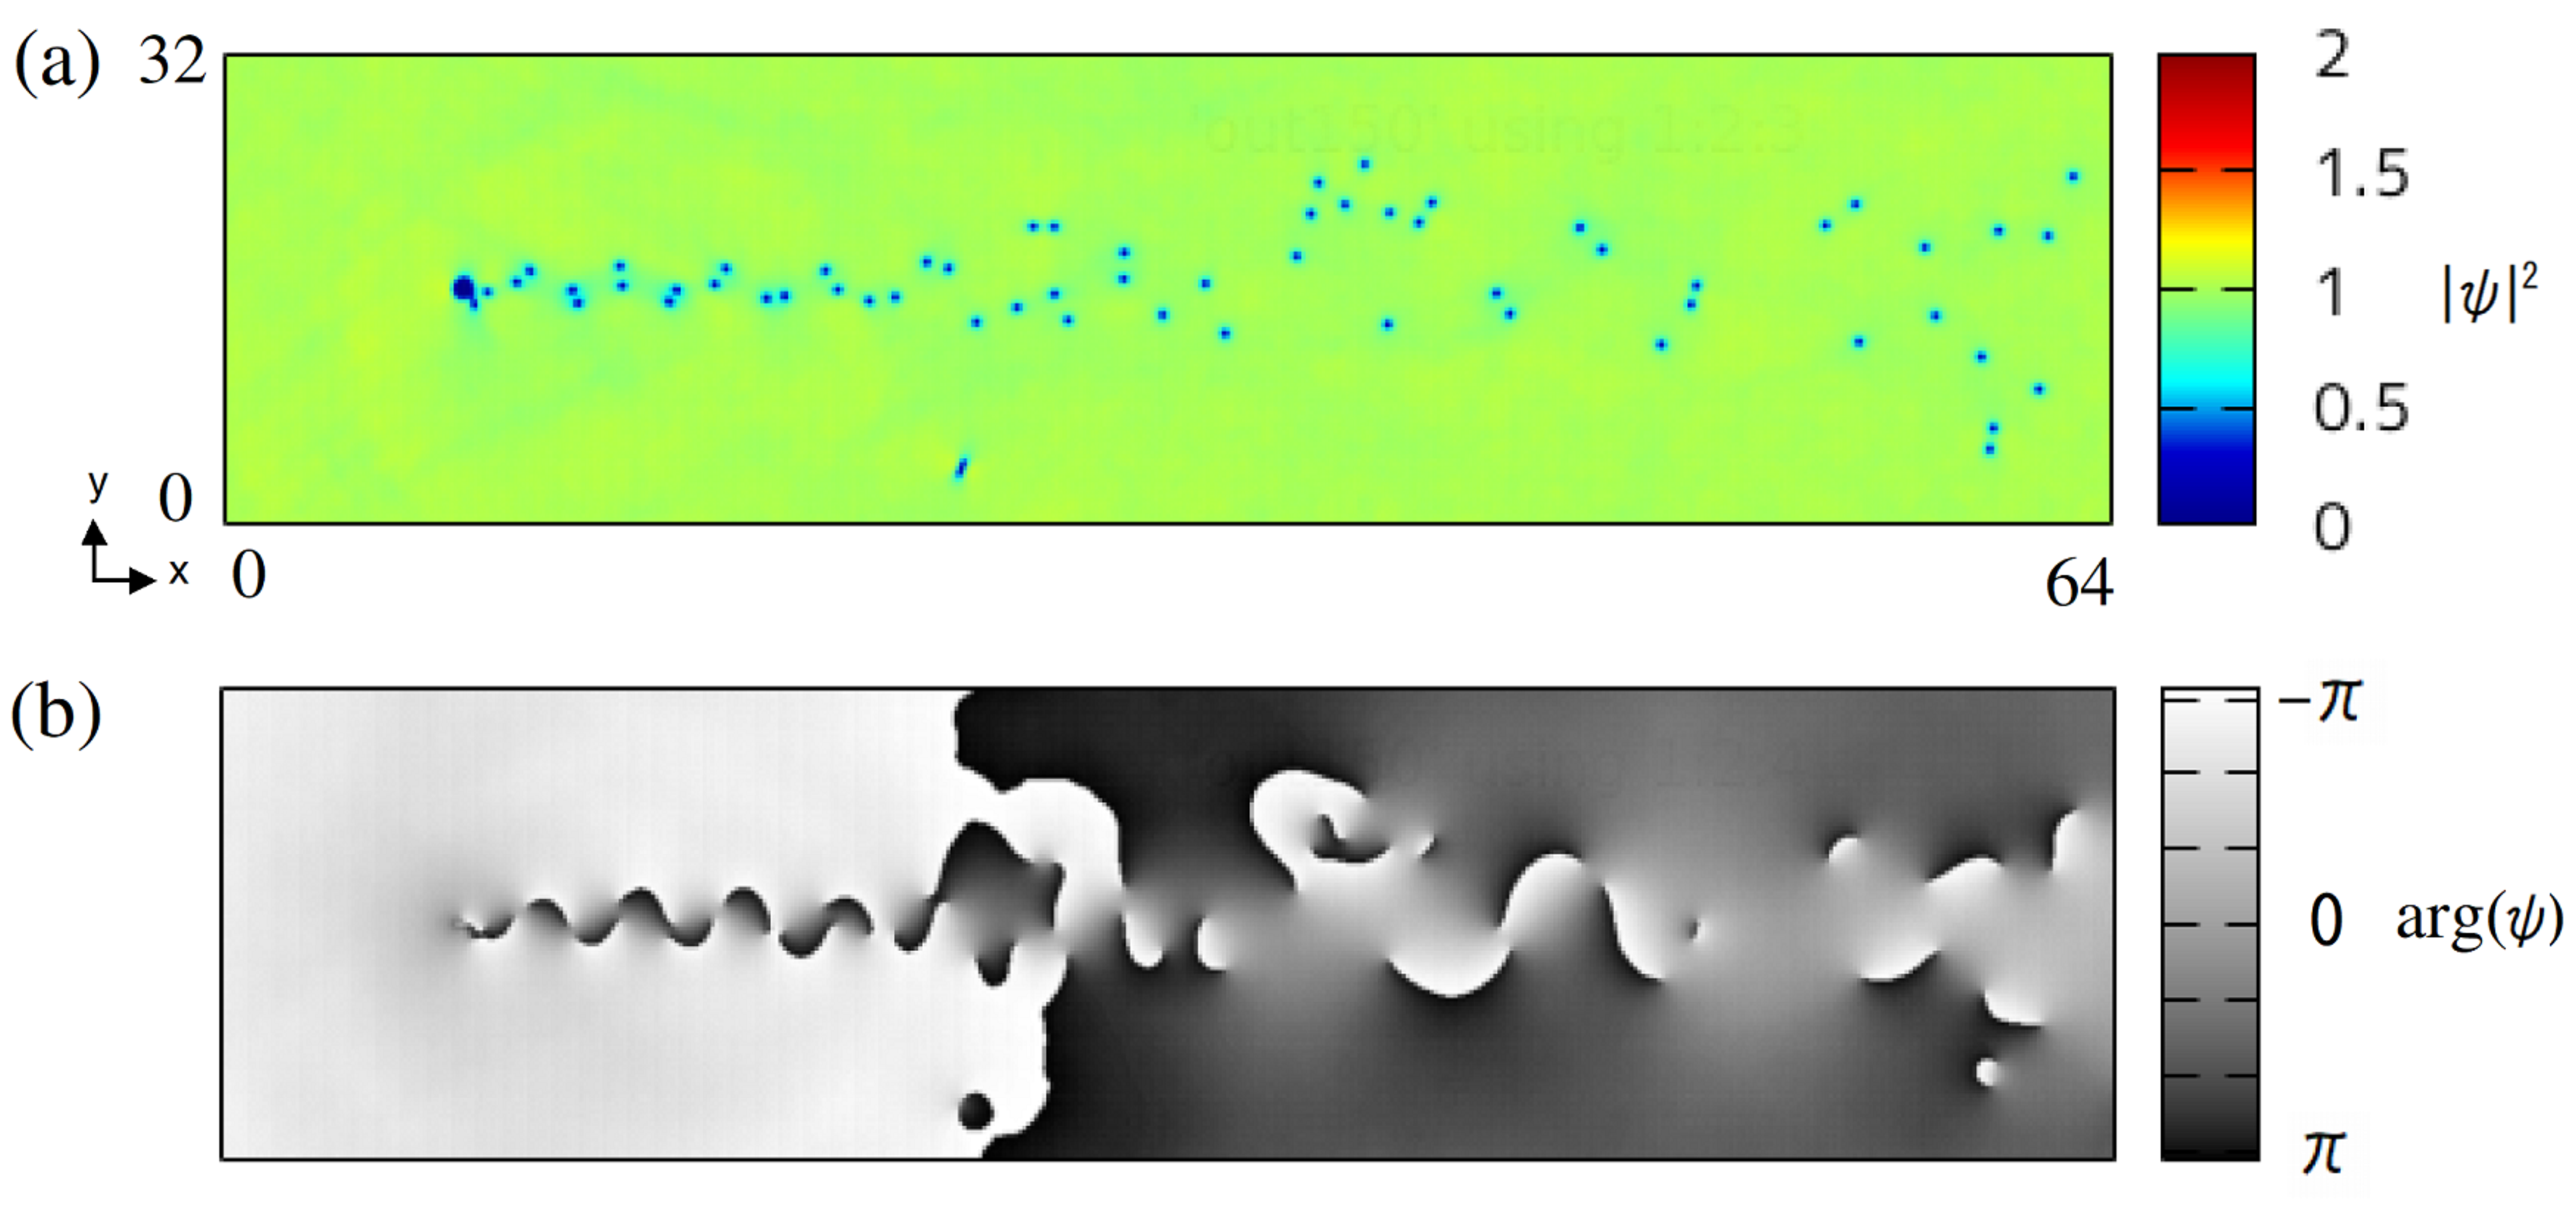
\includegraphics[width=16cm]{karman.eps}
				\caption{
					$(a)$は波動関数の確率密度、$(b)$は同時刻の位相を示す。
                    $(x,y)=(0 \sim 64, 0 \sim 32)$の二次元空間の一様な超流動体の中に、
		            円柱状の外部ポテンシャルが左方向へ一定速度で移動している状況である。
                    ポテンシャル後方に量子渦対が生成されながら、
					古典流体で見られるようなカルマン渦列の構成が見られる~\cite{Sasaki1}。
                    $(b)$の位相の図では量子渦の回転方向が交互の向きで、
                    くりかえしポテンシャルから生成している様子がわかる。
                    \\
		            K. Sasaki, N. Suzuki, and H. Saito,
                    \\
		            B\'enard--von K\'arm\'an vortex street in a Bose-Einstein condensate,
                    \\
		            Phys. Rev. Lett. \textbf{104}, 150404 (2010).
				}
				\label{FIG:karman}
			\end{center}
		\end{figure}
        量子渦の例として、トラップ中における量子渦の様子を
        図.~\ref{FIG:vortex}に示す。
        $(x,y)=(\pm8,\pm8)$の二次元系で、超流動体が
        直径$10$のガウシアン型トラップポテンシャルにより$0.7$の回転数で回した条件で、
        $6$個の量子渦が三角格子の配置で定常な状態をとる。
        数値計算は擬スペクトル法を用い、詳細は~\ref{s:numeric}(A)で示す。
        回転する古典流体ではみられるような系の境界サイズの大きな自由渦や強制渦の構造をとるが、
        超流動体では粘性をもたないため
        エネルギーが低い小さな渦が生成され、回転の中心から格子状に配置する。
        図.~\ref{FIG:vortex}(a)は密度$|\psi|^2$をあらわしピーク値が0.25を示す。また量子渦の
        箇所は急激に密度が低い状態であることが確認できる。
        図.~\ref{FIG:vortex}(b)では、真上から見た様子で三角格子の配置であることがわかる。
        図.~\ref{FIG:vortex}(c)は速度場をあらわし$6$個の量子渦それぞれが反時計回りで回り、
        全体でも反時計回りの回転を示している。
        図.~\ref{FIG:vortex}(d)は位相をあらわし$6$箇所にある量子渦で位相が$0 \sim 2\pi$に
        回転していることがわかる。

		\begin{figure}[H]
			\centering
			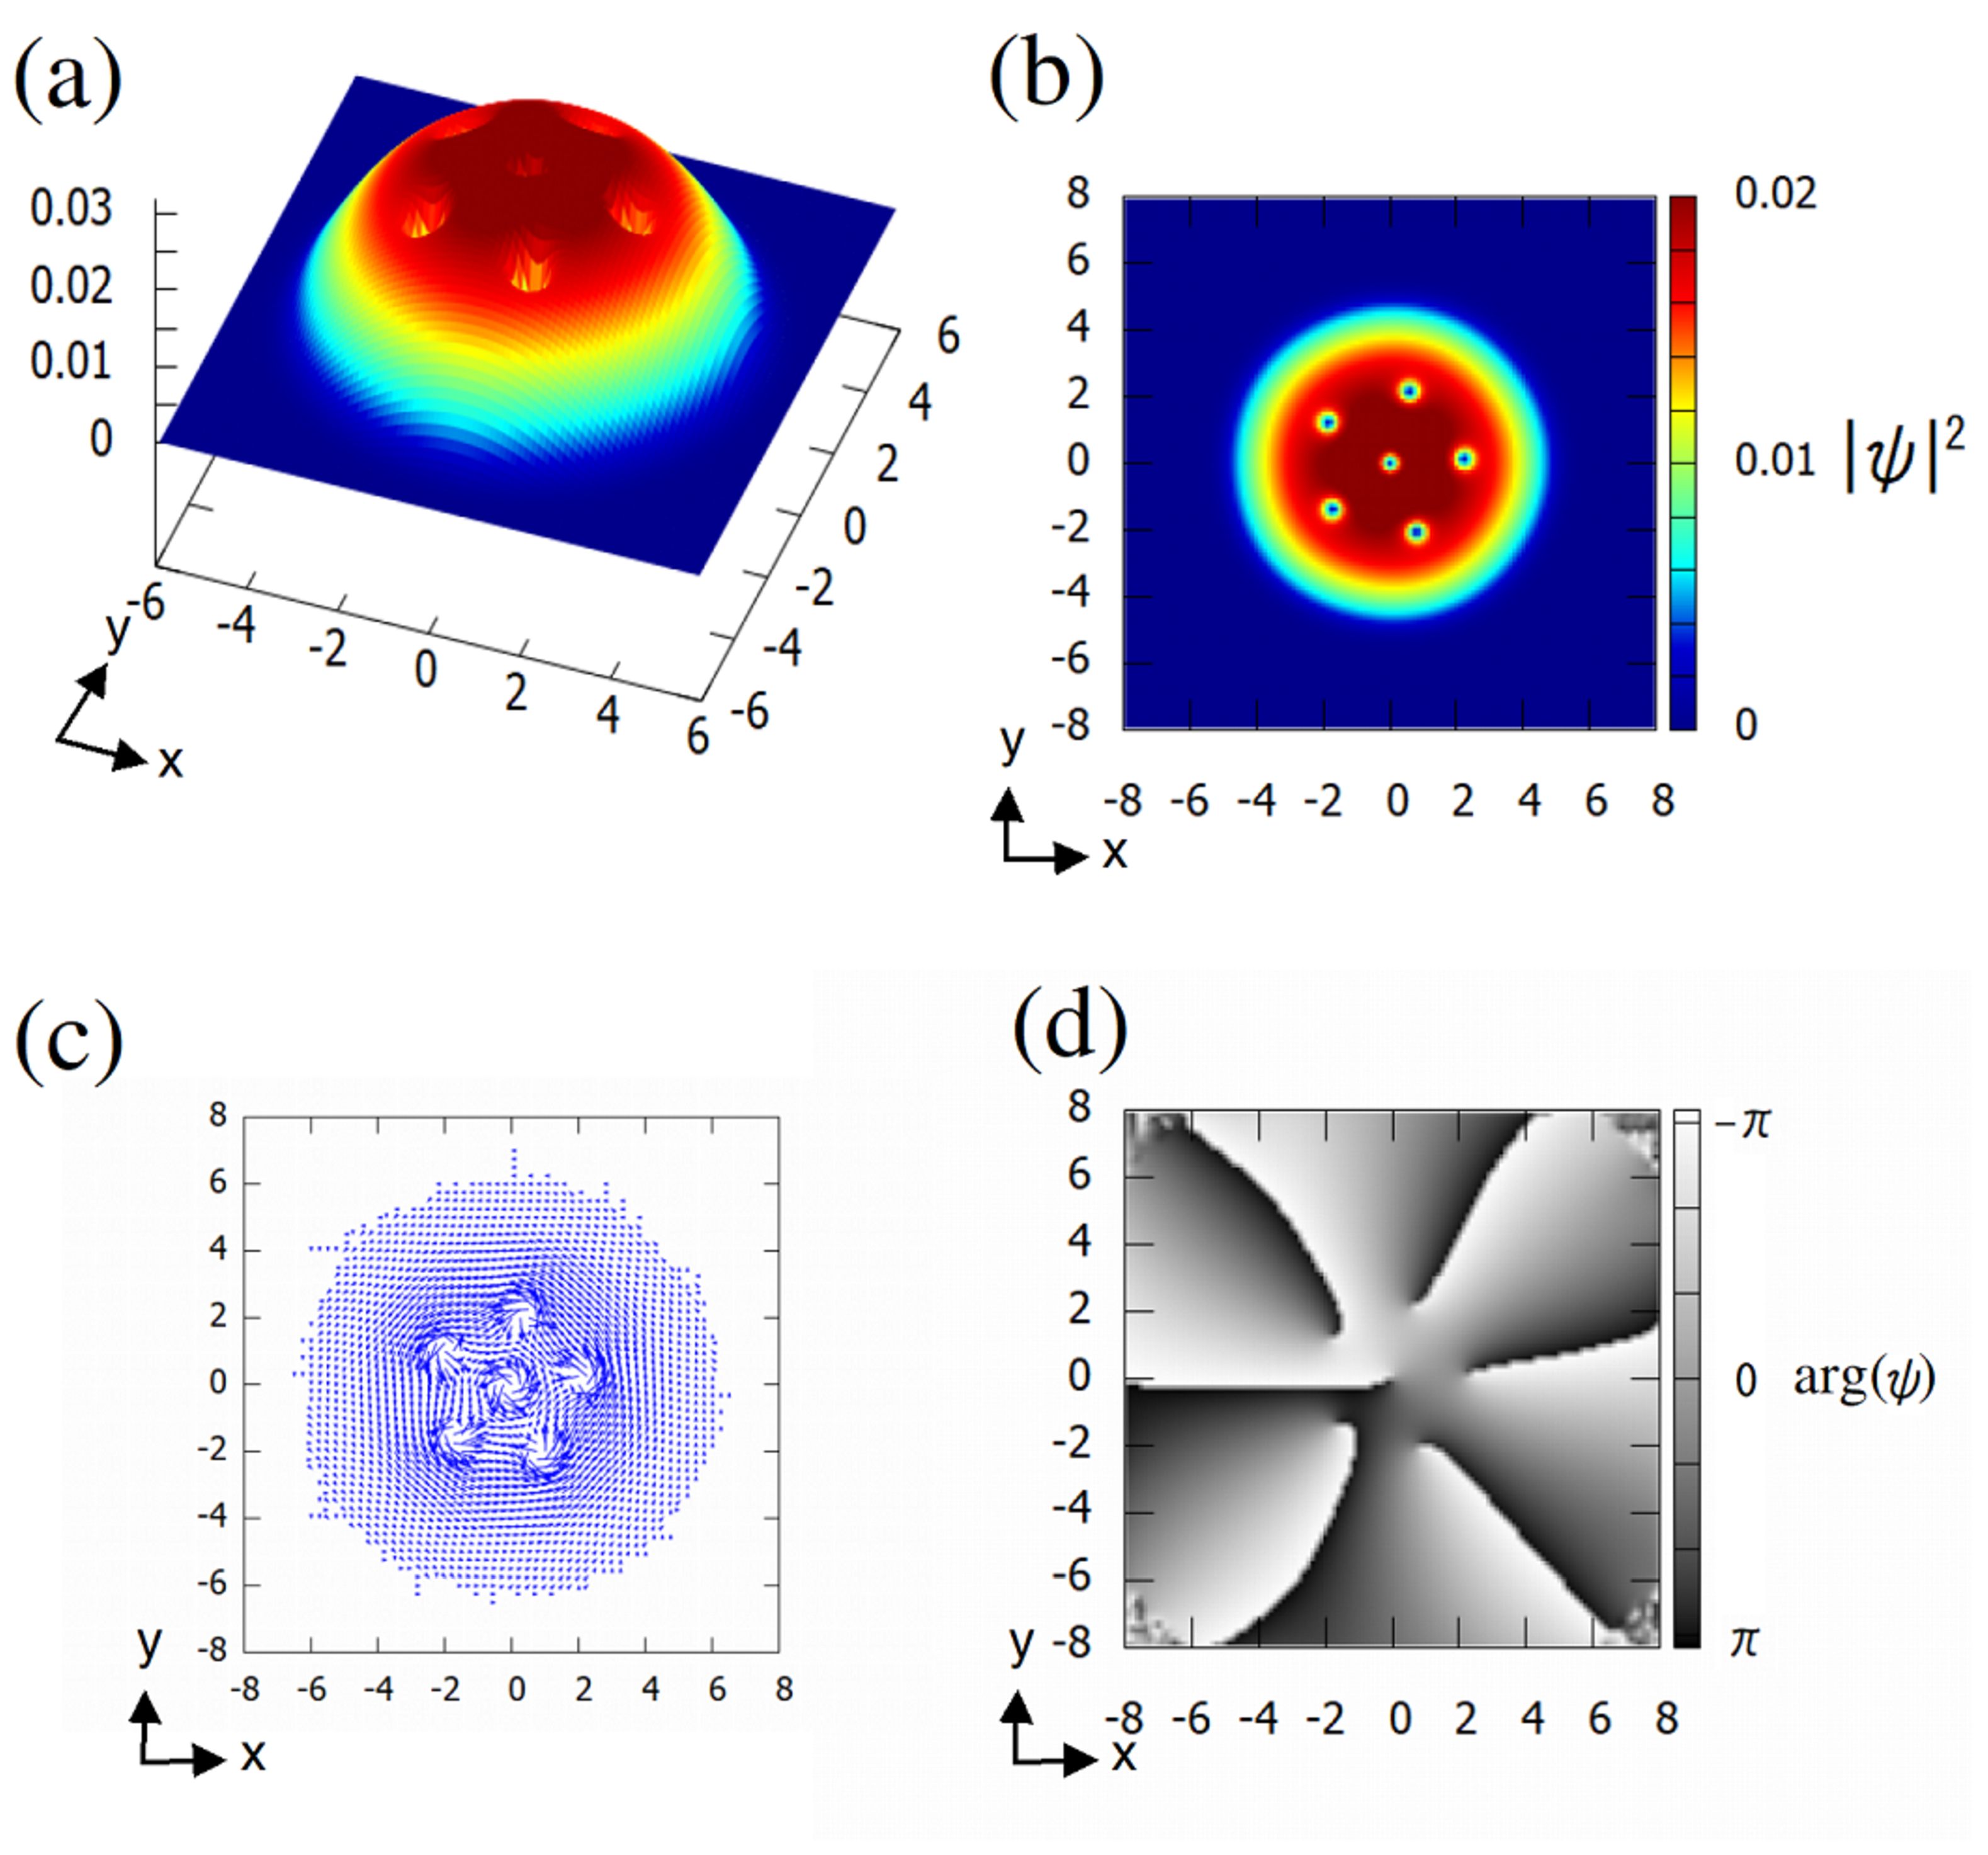
\includegraphics[width=14cm]{vortex.eps}
			\caption{
                (a)は密度$|\psi|^2$をあらわしピーク値が0.25を示す。また量子渦の
                箇所は急激に密度が低い状態であることが確認できる。
                (b)では、真上から見た様子で三角格子の配置であることがわかる。
                (c)は速度場をあらわし$6$個の量子渦それぞれが反時計回りで回り、
                全体でも反時計回りの回転を示している。
                (d)は位相をあらわし$6$箇所にある量子渦で位相が$0 \sim 2\pi$に
                回転していることがわかる。
                $(x,y)=(\pm8,\pm8)$の二次元系で
                直径$10$のガウシアン型ポテンシャルによりトラップされた超流動体を、
                $0.7$の回転数で回した場合の
                $6$個の量子渦が三角格子の配置で定常な状態になる条件で数値計算を行う。
                数値計算は擬スペクトル法を用いて算出した。
                詳細については~\ref{s:numeric}(A)にて示す。
			}
			\label{FIG:vortex}
		\end{figure}


		\section{渦対の移動速度}
        二次元の超流動体の渦は確率密度ゼロで、渦芯の境界では急激な密度勾配をもつため可視化の判断がしやすい。
        図.~\ref{FIG:internal}の例では、相生らの二次元系超流動体における渦対の運動を示す~\cite{Aioi0}。
        $(x,y)=(64,32)$の二次元の一様な超流動体に直径$5$、大きさ$5$の二つの引力ポテンシャルを
        $(x,y)=(0,11.2),(0.20.8)$の位置から
        $(x,y)=(0.5,11.2),(0.5.20.8)$の位置まで速度$0.01$で動かし、ポテンシャルの間から
        量子渦対を生成させる。
		反時計回りと時計回りのペアの渦を構成するものを渦対という。
        図.~\ref{FIG:internal}(a)では、$(x,y)=(40,16)$の位置に直径$2$、大きさ$1$の引力(青色)ポテンシャルを配置し、
        移動してきた量子渦対の渦間距離を短くさせて、加速させる。
        図.~\ref{FIG:internal}(b)では、$(x,y)=(40,16)$の位置に直径$2$、大きさ$-1$の斥力(赤色)ポテンシャルを配置し、
        移動してきた量子渦対の渦間距離を長くさせて、減速させる。
		渦対間の距離を$d$とすると、移動速度は$v_{\rm pair} \propto \log 1/d$で比例する。
		図の結果から渦対間距離が狭いほど進む速度は速いことがわかる。
		\begin{figure}[H]
			\centering
			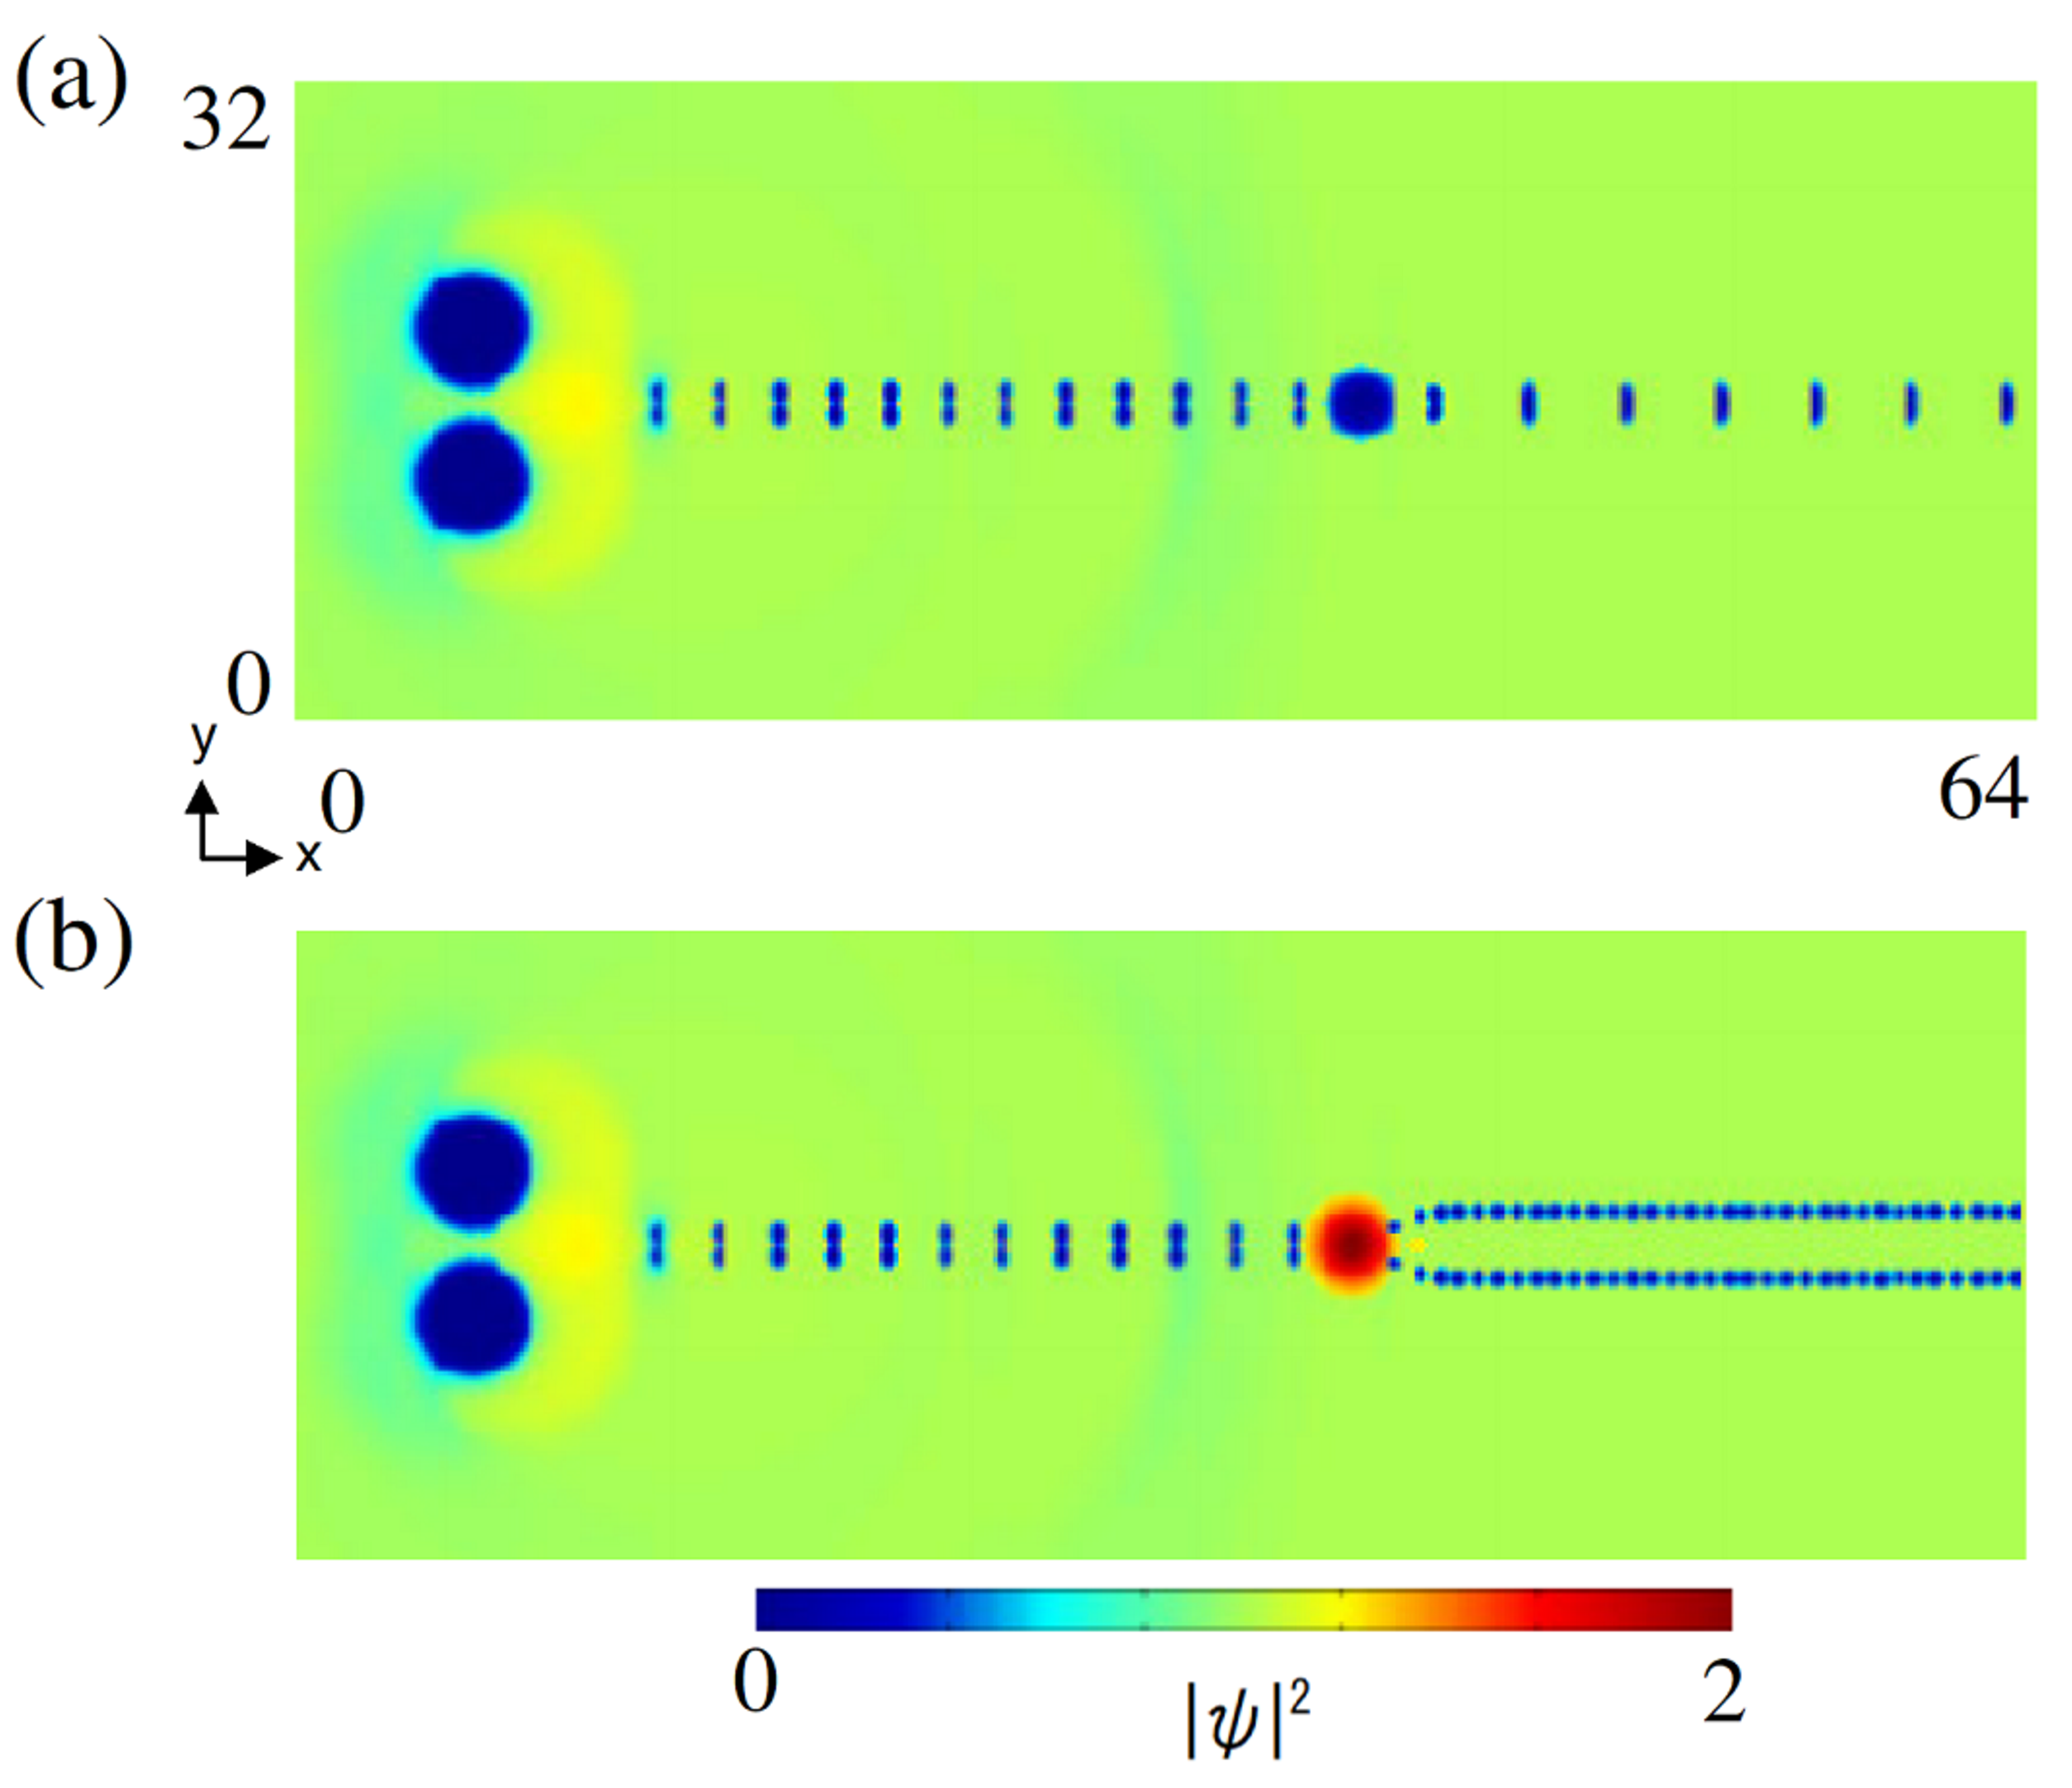
\includegraphics[width=13cm]{internal.eps}
			\caption{
                渦対が左から右に向かって移動した位置を、ストロボスコープのように
                一定のタイミングで重ねた図。
                $(x,y)=(64,32)$の二次元の一様な超流動体に直径$5$、大きさ$5$の二つの引力ポテンシャルを
                $(x,y)=(0,11.2),(0.20.8)$の位置から
                $(x,y)=(0.5,11.2),(0.5.20.8)$の位置まで速度$0.01$で動かし、ポテンシャルの間から
                量子渦対を生成させる。
                その後(a)では、$(x,y)=(40,16)$の位置に直径$2$、大きさ$1$の引力(青色)ポテンシャルを配置し、
                移動してきた量子渦対の渦間距離を短くさせて、加速させる。
                (b)では、$(x,y)=(40,16)$の位置に直径$2$、大きさ$-1$の斥力(赤色)ポテンシャルを配置し、
                移動してきた量子渦対の渦間距離を長くさせて、減速させる。
			    (a)では量子渦が引力ポテンシャルを通過した後、渦間距離が狭く変化し移動速度が上がる。
			    (b)では量子渦が斥力ポテンシャルを通過した後、渦間距離が広く変化し移動速度が下がる~\cite{Aioi0}。
                \\
		        T. Aioi, T. Kadokura, T. Kishimoto, and H. Saito,
                \\
		        Controlled generation and manipulation of vortex dipoles in a Bose-Einstein condensate, 
                \\
		        Phys. Rev. X{\bf 1}, 021003 (2011).
			}
			\label{FIG:internal}
		\end{figure}


        \section{音速}
        量子流体力学における連続の式~(\ref{eq:qcont})とオイラー方程式~(\ref{eq:qeuler})から
        \begin{eqnarray}
            \frac{\partial^2}{\partial t^2}n_0
            & = & \left( \frac{g n_0}{m^2} \right) \Vec{\nabla}^2 n_0
            - \left( \frac{\hbar^2}{4m} \right) \Vec{\nabla}^4 n_0,
        \end{eqnarray}
        が得られ
        右辺の第二項の4次の空間微分を$0$に近似し、
        \begin{eqnarray}
            \frac{\partial^2}{\partial t^2} n_0 = c^2 \Vec{\nabla}^2 n_0,
        \end{eqnarray}
        の波動方程式をあらわす。ここで、
        \begin{eqnarray}
            c = \sqrt{\frac{g n_0}{m^2}},
        \end{eqnarray}
		は超流動体における音速$c$を示す。


        例として図.~\ref{FIG:criticalv}は、
        $(x,y)=(\pm1,\pm1)$の二次元の一様な超流動体に
        直径$0.2$の円形ポテンシャルを$(x,y)=(0,0)$に配置し、
        左から右に向かって音速に近い流れを与えた様子を示す。
        図.~\ref{FIG:criticalv}(a)は密度$|\psi|^2$をあらわし、
        ポテンシャルの後方には密度がほぼゼロの領域があり、
        前方から斜め後方に向かって角度のついた密度の大きな波が生じている。
        図.~\ref{FIG:criticalv}(b)の位相からは量子渦が存在していないことが確認される。
        図.~\ref{FIG:criticalv}(c)の速度場では、円形ポテンシャル後方の密度が小さい方向に
        向かって速度ベクトルが向き、密度が小さい方向に流れていることがわかる。
        数値計算は擬スペクトル法を用いて算出した。
        詳細については~\ref{s:numeric}(A)にて示す。
        %音速$c$は~(\ref{eq:elem})の$k\rightarrow 0$の極限における超流動の臨界速度を与えるが、
        %実際の実験系ではこれよりも小さい速度で不安定になることが知られており、
        %自由粒子系の任意の$k$に対する
        %運動エネルギー$\epsilon_{k} = \frac{\hbar^2 k^2}{2m}$であらあわされる。
		\begin{figure}[H]
			\begin{center}
				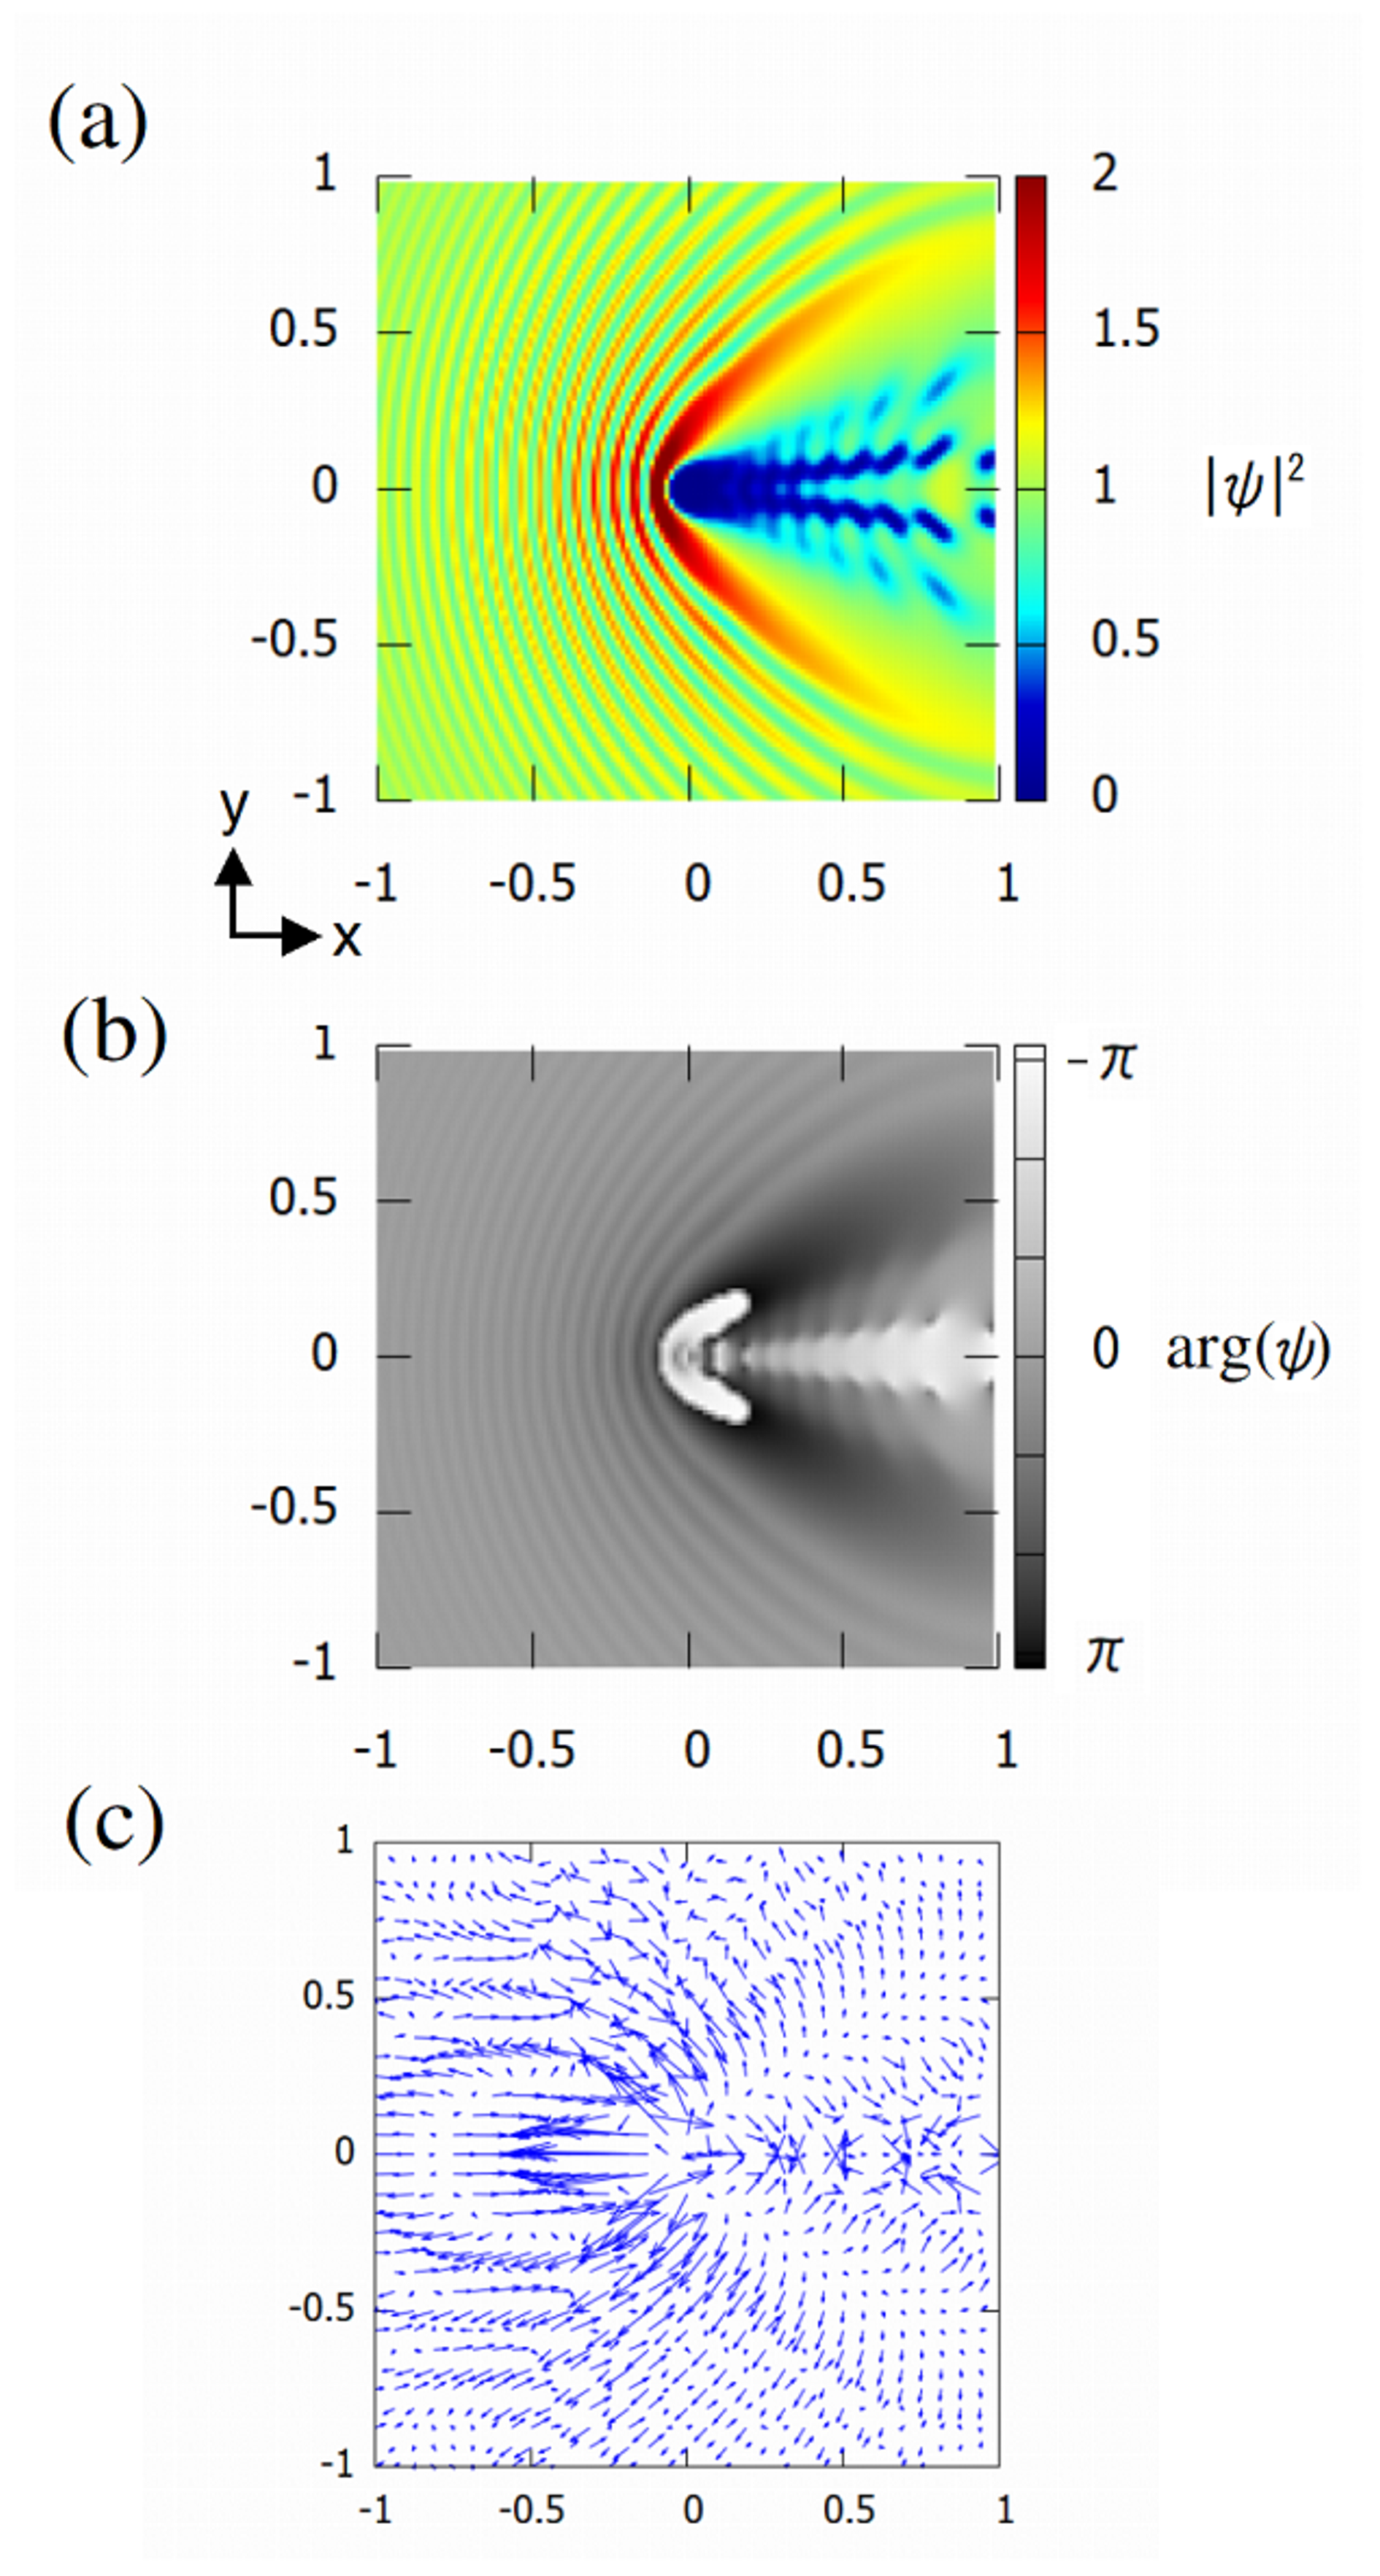
\includegraphics[width=10cm]{criticalv.eps}
				\caption{
					それぞれ(a)は密度、(b)は同時刻の位相、
					(c)は速度場をあらわす。
                    $(x,y)=(\pm1,\pm1)$の二次元の一様な超流動体に
                    直径$0.2$の円形ポテンシャルを$(x,y)=(0,0)$に配置し、
                    左から右に向かって音速付近の流れを与えた様子を示す。
                    (a)では
                    ポテンシャルの後方には密度がほぼゼロの領域があり、
                    前方には角度のついた密度の大きな波が生じている。
                    (b)の位相では量子渦が存在していないことが確認される。
                    (c)の速度場では、円形ポテンシャル後方の密度が小さい方向に
                    向かって速度ベクトルが向き、密度が小さい方向に流れていることがわかる。
                    数値計算は擬スペクトル法を用いて算出した。
                    詳細については~\ref{s:numeric}(A)にて示す。
				}
				\label{FIG:criticalv}
			\end{center}
		\end{figure}
		%また門倉らの量子渦生成の双安定性の研究では、
        %加速時の渦生成の開始速度が、減速時の渦生成がしなくなる速度と同じではなく、
        %双安定性を持つことが確認されている~\cite{hysteresis}。
        %例として図.~\ref{FIG:hysteresis}は、
        %二次元の空間$(x,y)=(512,256)$の大きさの
        %周期的境界条件を課した空間に一様に超流動がある系で、
        %半径$5.1$、大きさ$1$の引力ポテンシャルを$-x$方向に移動させている様子である。
        %図.~\ref{FIG:hysteresis}(a)から(d)では、$(x,y)=(80,40)$の部分を拡大して見ている。
        %図.~\ref{FIG:hysteresis}(a)で示すポテンシャルの$y$軸上の、上下から交互に量子渦が生成し
        %(a)~(d)までの時間発展の様子から右側の位相の図を見ると
        %生成された量子渦が時計回りと反時計回りの二つペアであることがわかる。
        %図.~\ref{FIG:hysteresis}(e)では、ポテンシャルの$y$軸上の上側の箇所の
        %$x$方向の速度のグラフをあらわし、赤線は加速時、青線は減速時を示す。
        %
		%\begin{figure}[H]
		%	\begin{center}
		%		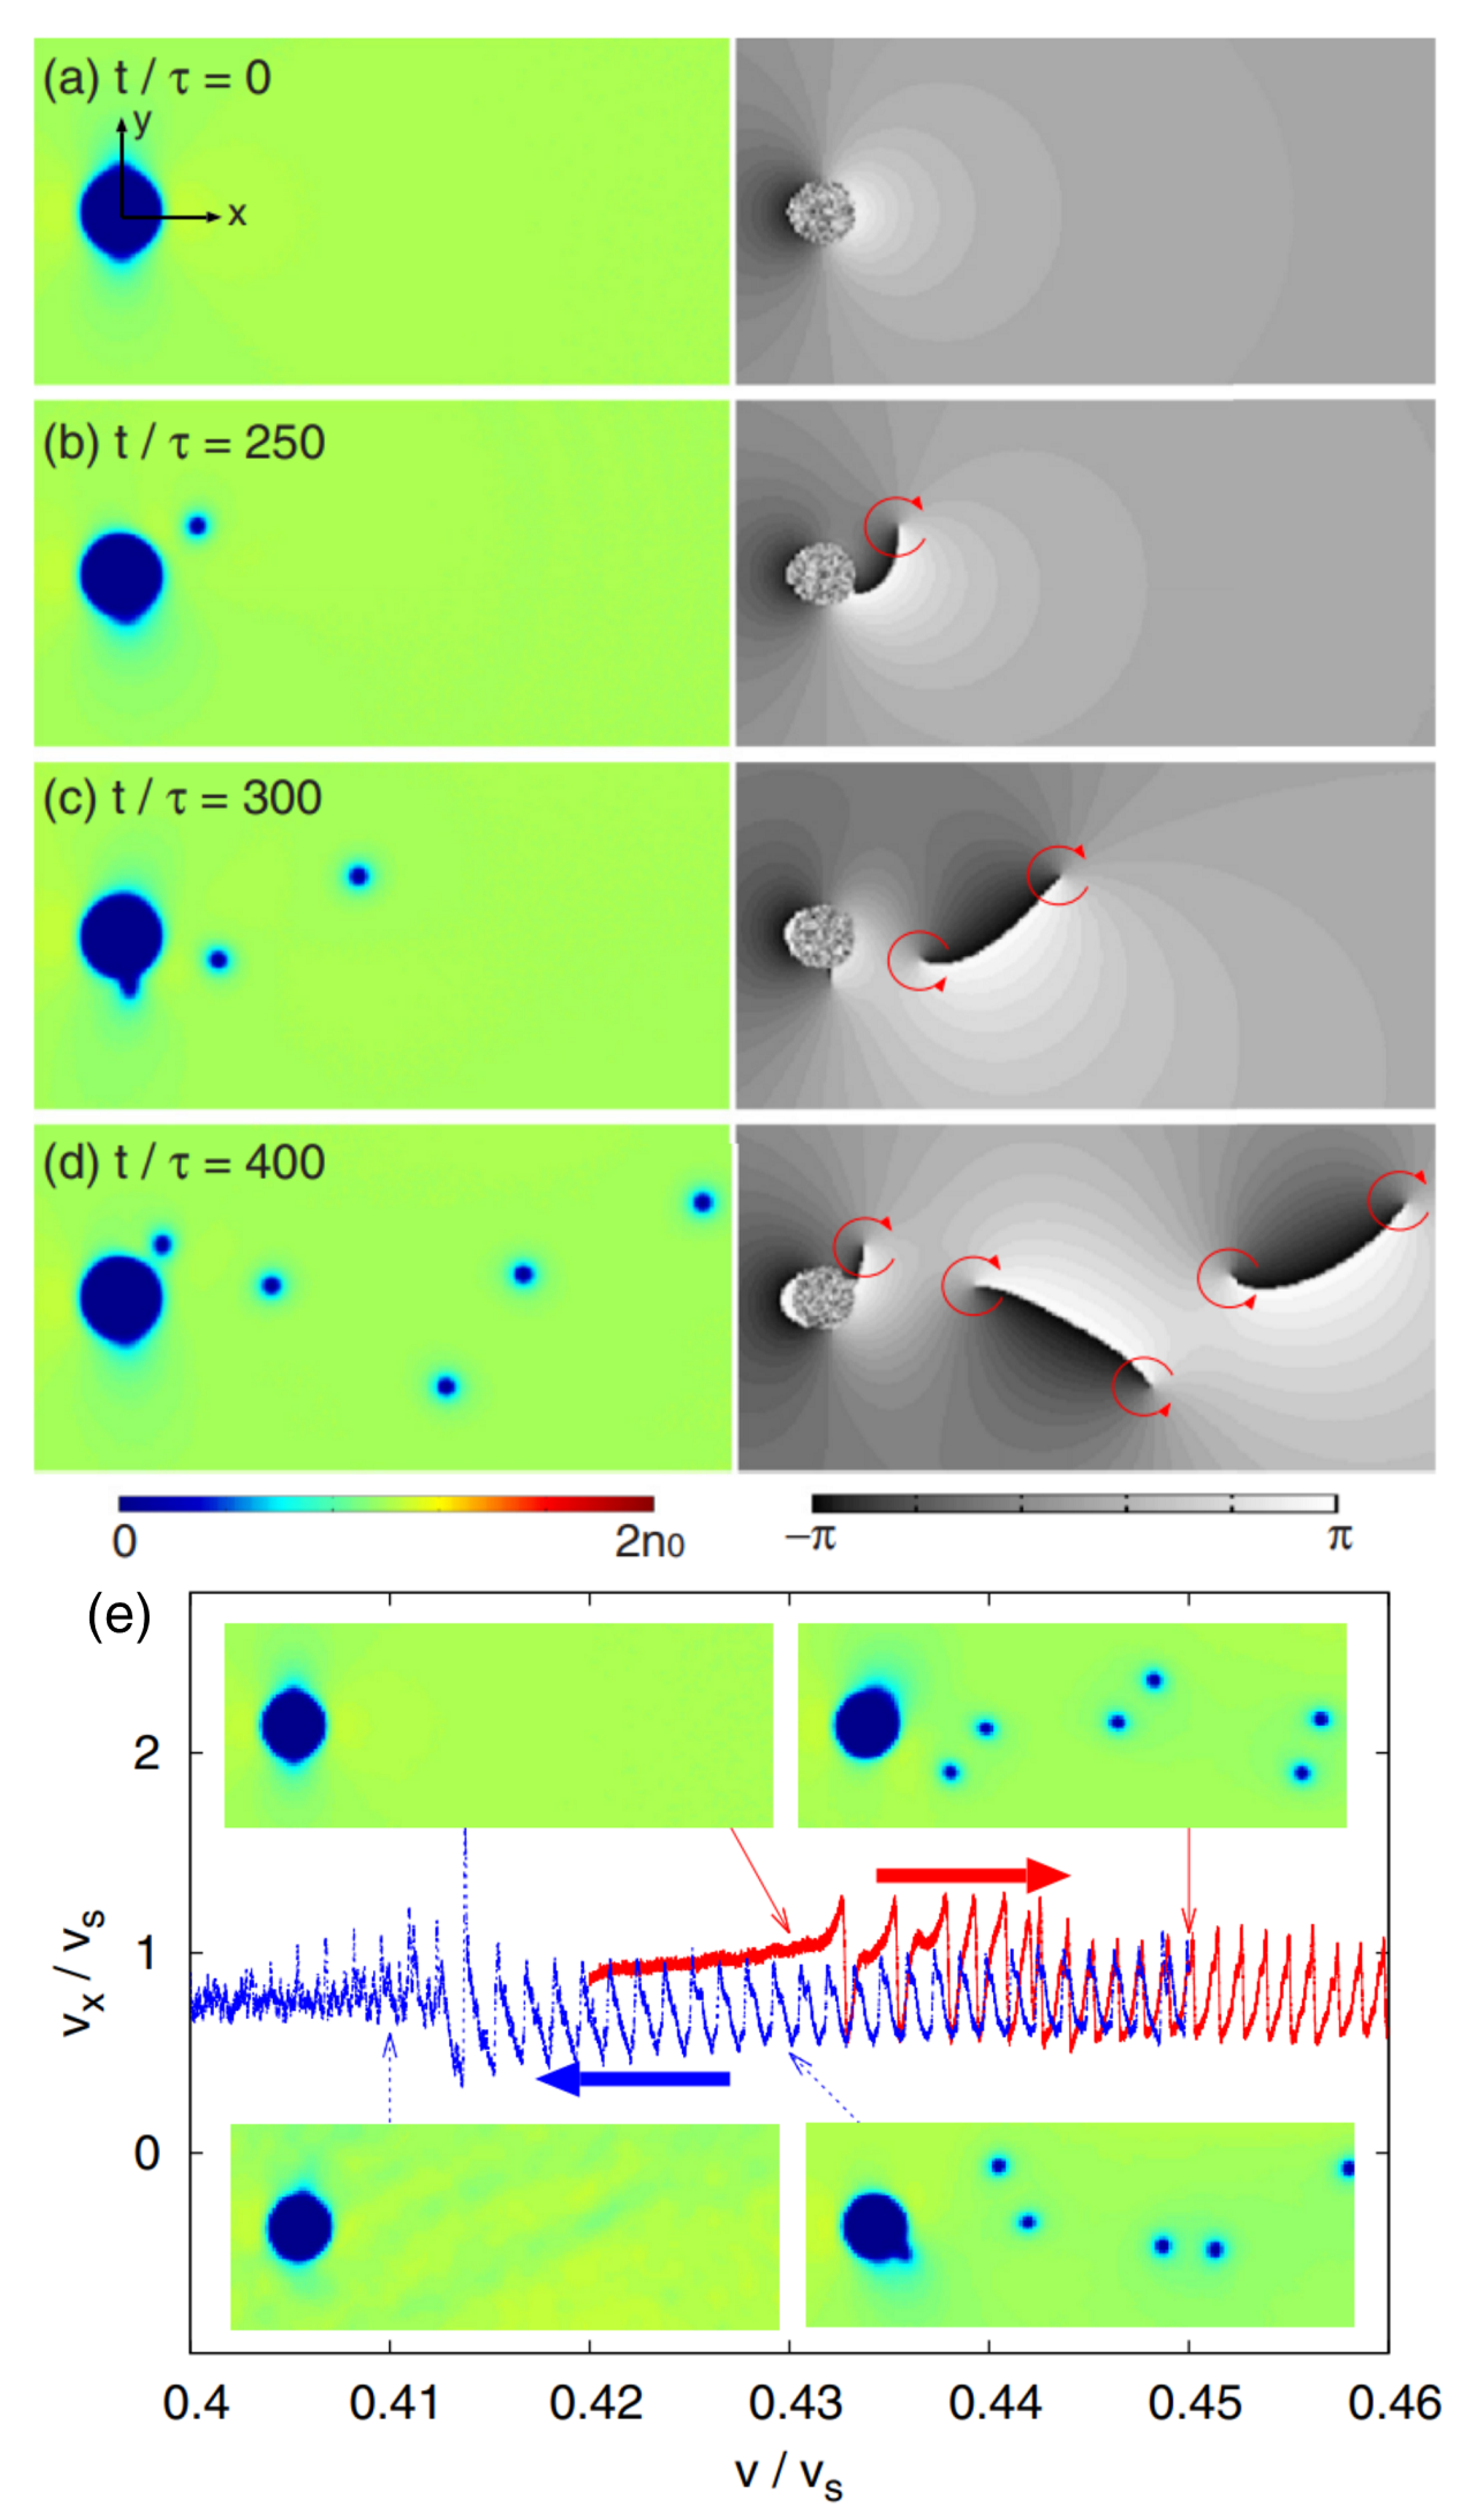
\includegraphics[width=12cm]{hysteresis.eps}
		%		\caption{
		%			(a)~(d)は渦対生成の時間発展の確率密度$|\psi|^2$と位相、
        %            (e)は渦対生成の加速時、減速時の双安定性を示す。
        %            二次元の空間$(x,y)=(512,256)$の大きさの
        %            周期的境界条件を課した空間に一様に超流動がある系で、
        %            半径$5.1$、大きさ$1$の引力ポテンシャルを$-x$方向に移動させている様子である。
        %            (a)から(d)では、$(x,y)=(80,40)$の部分を拡大して見ている。
        %            (a)で示すポテンシャルの$y$軸上の、上下から交互に量子渦が生成し
        %            (a)~(d)までの時間発展の様子から右側の位相の図を見ると
        %            生成された量子渦が時計回りと反時計回りの二つペアであることがわかる。
        %            では、ポテンシャルの$y$軸上の上側の箇所の
        %            $x$方向の速度のグラフをあらわし、赤線は加速時、青線は減速時を示す。
        %            $v/v_s$は円柱ポテンシャルの移動速度と超流動体の相対速度、
        %            $v_x/v_s$は円柱ポテンシャルの$12$時の位置と超流動体の相対速度。
        %            渦対は繰り返し生成され、その生成の開始速度は停止速度よりも速い値を示している~\cite{hysteresis}。
        %            \\
		%            Tsuyoshi Kadokura, Jun Yoshida, and Hiroki Saito,
        %            \\
		%            Hysteresis in quantized vortex shedding,
        %            \\
		%            Phys. Rev. A {\bf 90}, 013612 (2014).
		%		}
		%		\label{FIG:hysteresis}
		%	\end{center}
		%\end{figure}


		\section{量子乱流とエネルギーカスケード}
        図.~\ref{FIG:turbulent}は量子流体が発達した一様等方性乱流に至るまでの時間発展の様子を示す。
        系は$(x,y,z)=(\pm64,\pm64,\pm64)$の三次元空間で周期的境界条件を課してある。
	    図.~\ref{FIG:turbulent}(a)--(c)は量子乱流中の渦芯(緑色)とランダムポテンシャルの等値面(青色)の時間発展、
        図.~\ref{FIG:turbulent}(a$'$)--(c$'$)は同時刻のエネルギースペクトル、
        図.~\ref{FIG:turbulent}(a$''$)--(c$''$)は同時刻の確率密度$|\psi|^2$の断面$(z=0)$の様子。
        ランダムポテンシャルがつくりだす外力によって流体がかきまぜられ、
        発達した定常乱流の状態になり
        エネルギースペクトルは$-5/3$べき乗のコルモゴロフ則をとる。
        図.~\ref{FIG:turbulent}(c)の定常乱流の状態では、量子渦が空間中にランダムに運動する様子が見られる。
        量子渦は乱流における慣性領域のエネルギーカスケードで重要な役割を持つことがわかった。
        小スケール渦の生成過程とエネルギーカスケードの詳細については~\ref{c:orth}章で述べる。
		\begin{figure}[H]
			\centering
			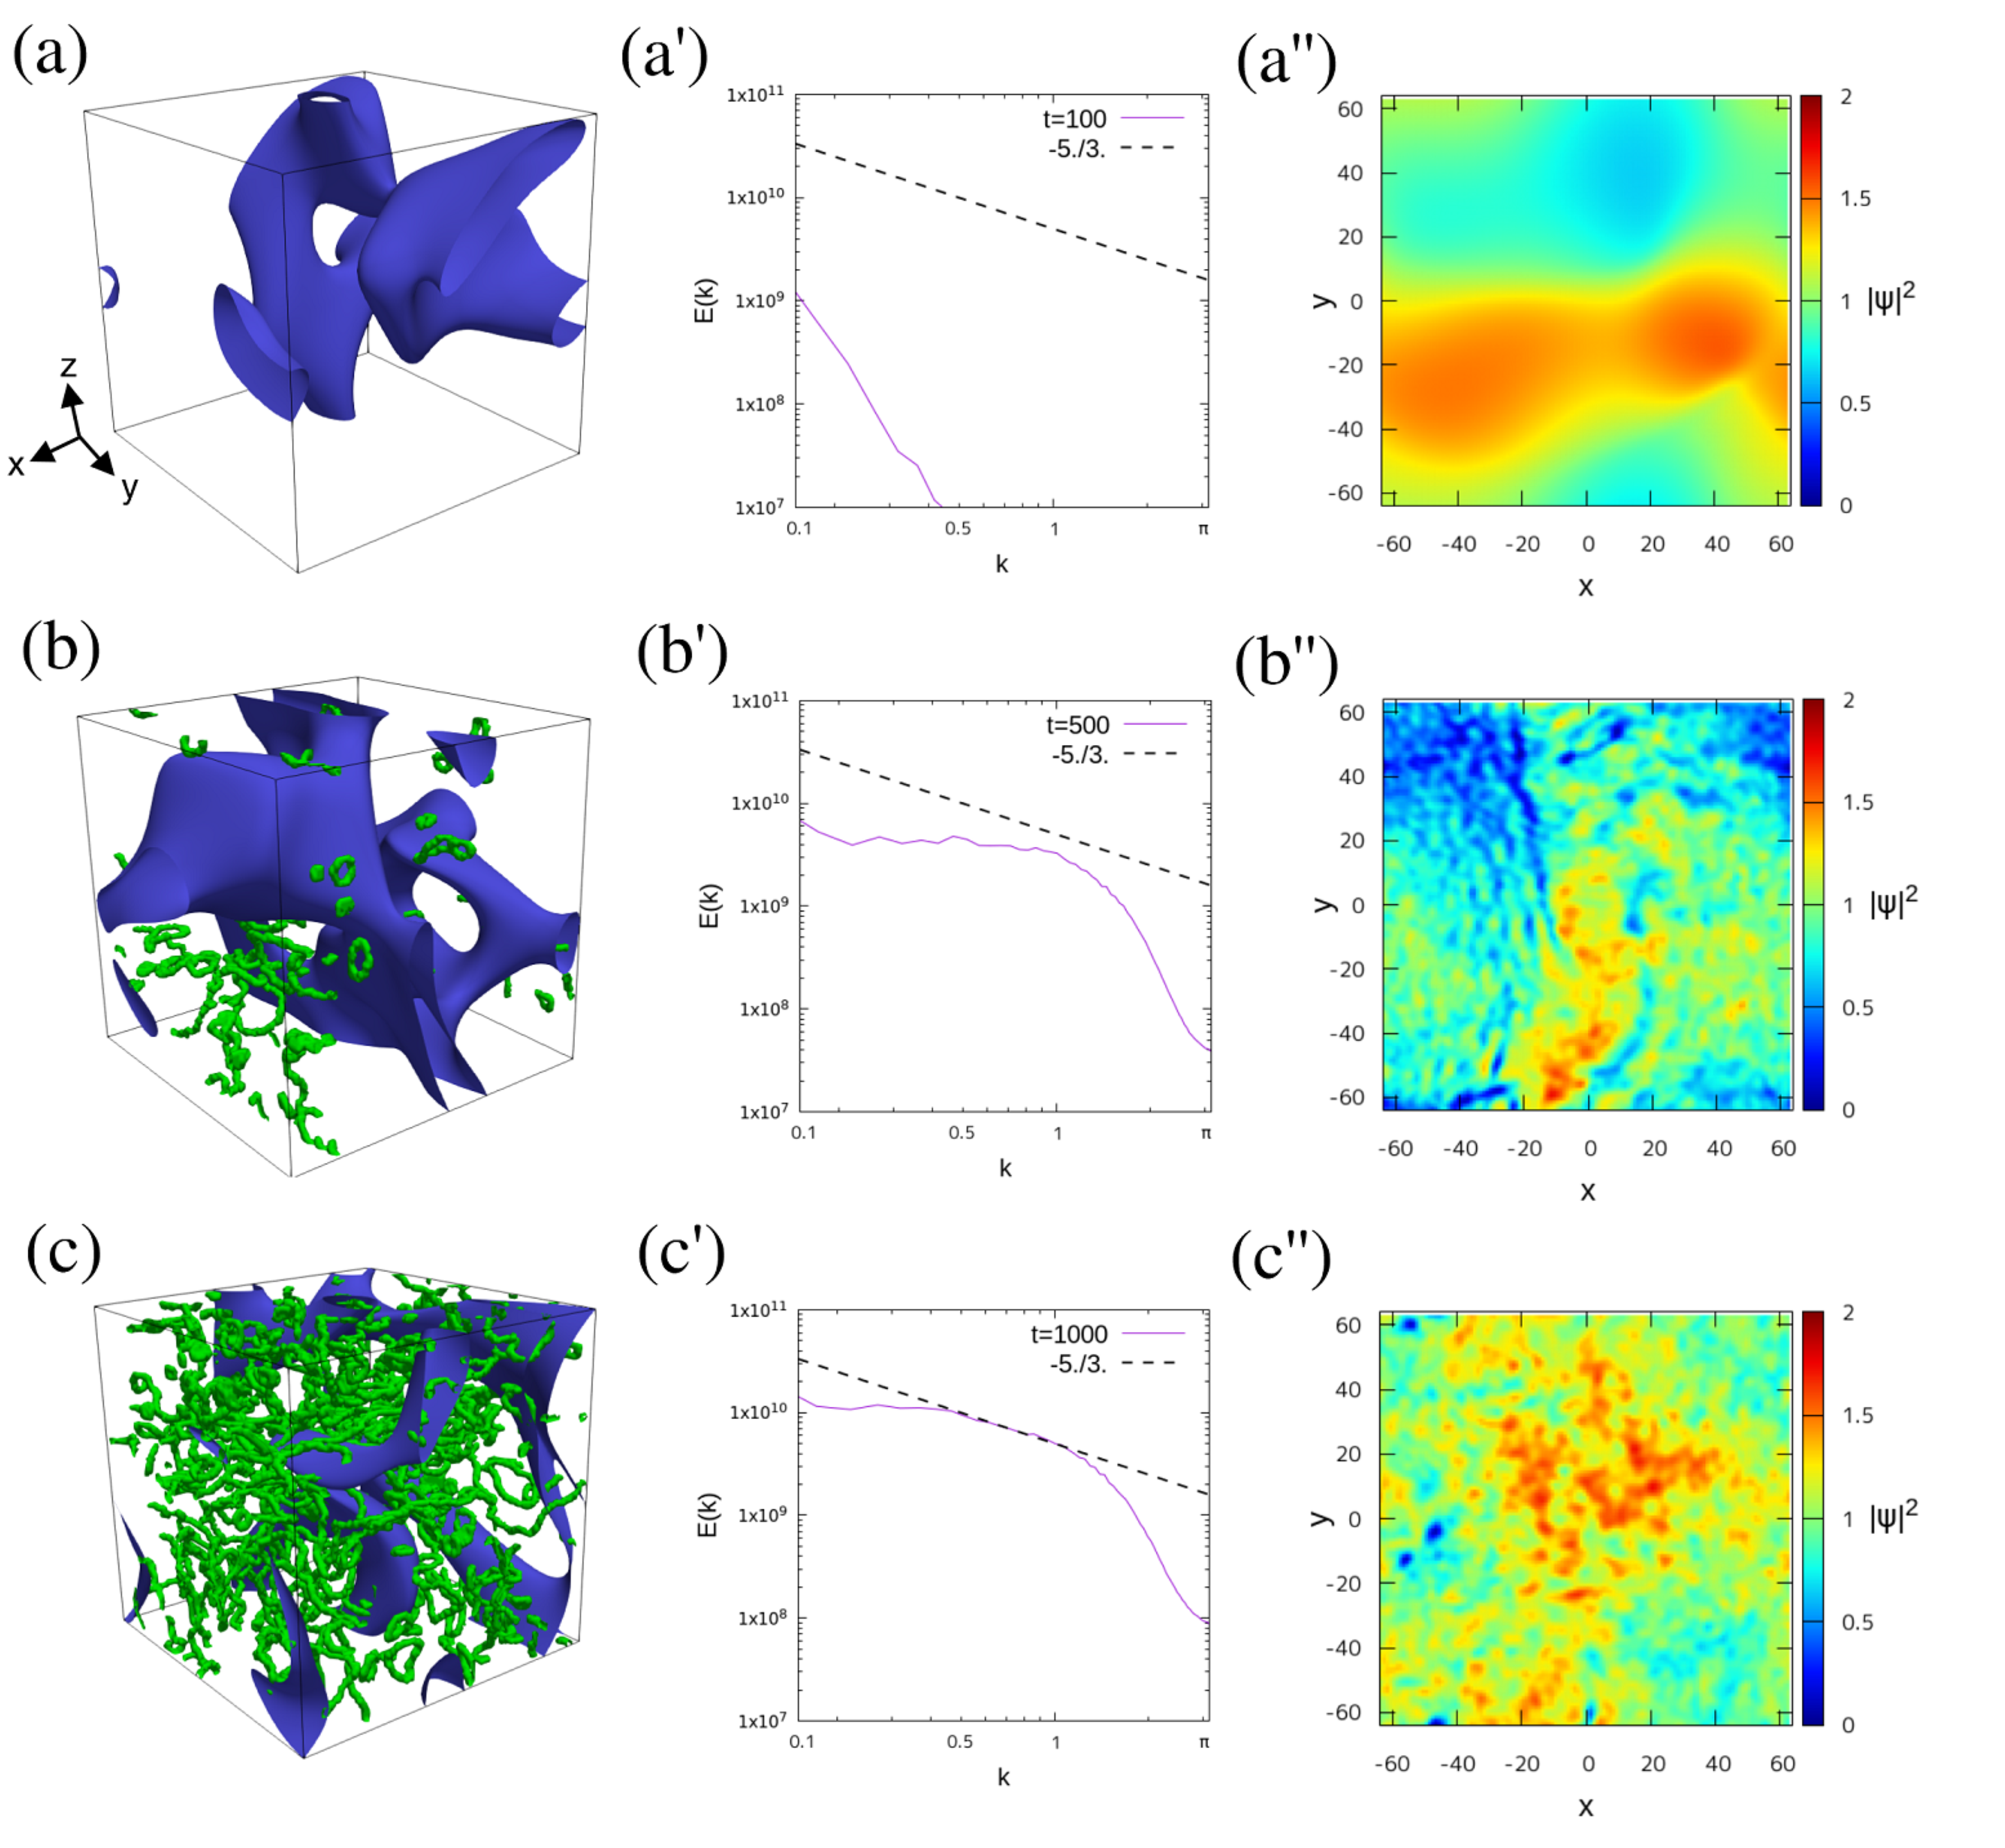
\includegraphics[width=16cm]{turbulent.eps}
			\caption{
			    (a)--(c)は量子乱流中の渦芯(緑色)とランダムポテンシャルの等値面(青色)の時間発展、
                (a$'$)--(c$'$)は同じ時刻のエネルギースペクトル、
                (a$''$)--(c$''$)は同じ時刻の確率密度$|\psi|^2$の断面$(z=0)$の様子。
                系は$(x,y,z)=(\pm64,\pm64,\pm64)$の三次元空間で周期的境界条件を課してある。
                ランダムポテンシャルがつくりだす外力により、発達した定常乱流の状態になると、
                エネルギースペクトルは$-5/3$べき乗のコルモゴロフ則となる。
                定常乱流により量子渦がランダムな運動をする。
                詳細は本論文の~\ref{c:orth}章を参照。
                数値計算は擬スペクトル法を用いて算出した(~\ref{s:numeric}(A))。
			}
			\label{FIG:turbulent}
		\end{figure}


		\section{むすび}
		この章では、本研究で必要となる知見のボース・アインシュタイン凝縮の
        歴史的背景を含めた概略と、量子流体、量子乱流の特徴について述べた。
		本研究では量子乱流における渦度の階層構造を分析する上で、
        エネルギースペクトルによる慣性領域での
        エネルギーカスケードの確認のほか、渦度分布を抽出による大小スケールの位置関係の分析、
        渦芯の可視化による渦バンドルのカスケードのダイナミクスの考察など
        多面的に試行し物理の信憑性を高めた。
        また流滴サイズ、エネルギー注入率の定量分析はそれまでの試行で得られた
        方法をもとに算出、考察を行った。第2章以降では古典流体も含めた乱流の
        先行研究、続いて量子乱流について本研究の内容とその成果について述べていく。


%%%%%%%%%%%% CHAPTER 2 %%%SECOND%%%%%%%%%%%%%%%%%%%%%%%%%%%%%%%%%%%%%%%%%%%%%%%%
	\chapter{乱流研究の概説}
		\section{まえがき}
		\ 古典流体の乱流の記録について、古くは
        図.~\ref{FIG:galileo}(a)にあるような、$16$世紀のガリレオが描いたスケッチが存在し、
        当時の科学において興味の対象であったことが頷ける。
        図.~\ref{FIG:galileo}(b)にあるように現在でも条件が近い同様の現象を我々は目にすることができる。
		乱流研究の歴史が進み、レイノルズはガラス管にながれる水流にインクを流し、
        可視化によって定量的な調査が行われ、慣性力と粘性の比から層流から乱流の程度を示すレイノルズ数が定義された。
        リチャードソンは、乱流中の大規模渦から小規模渦が分裂生成される過程を物理的な描像を句で記し、
        コルモゴロフによる統計を用いた乱流のエネルギーカスケードの発見に至る。
		近年では二次元や三次元、多成分など多岐に渡った研究が行われている。
		\begin{figure}[H]
			\centering
			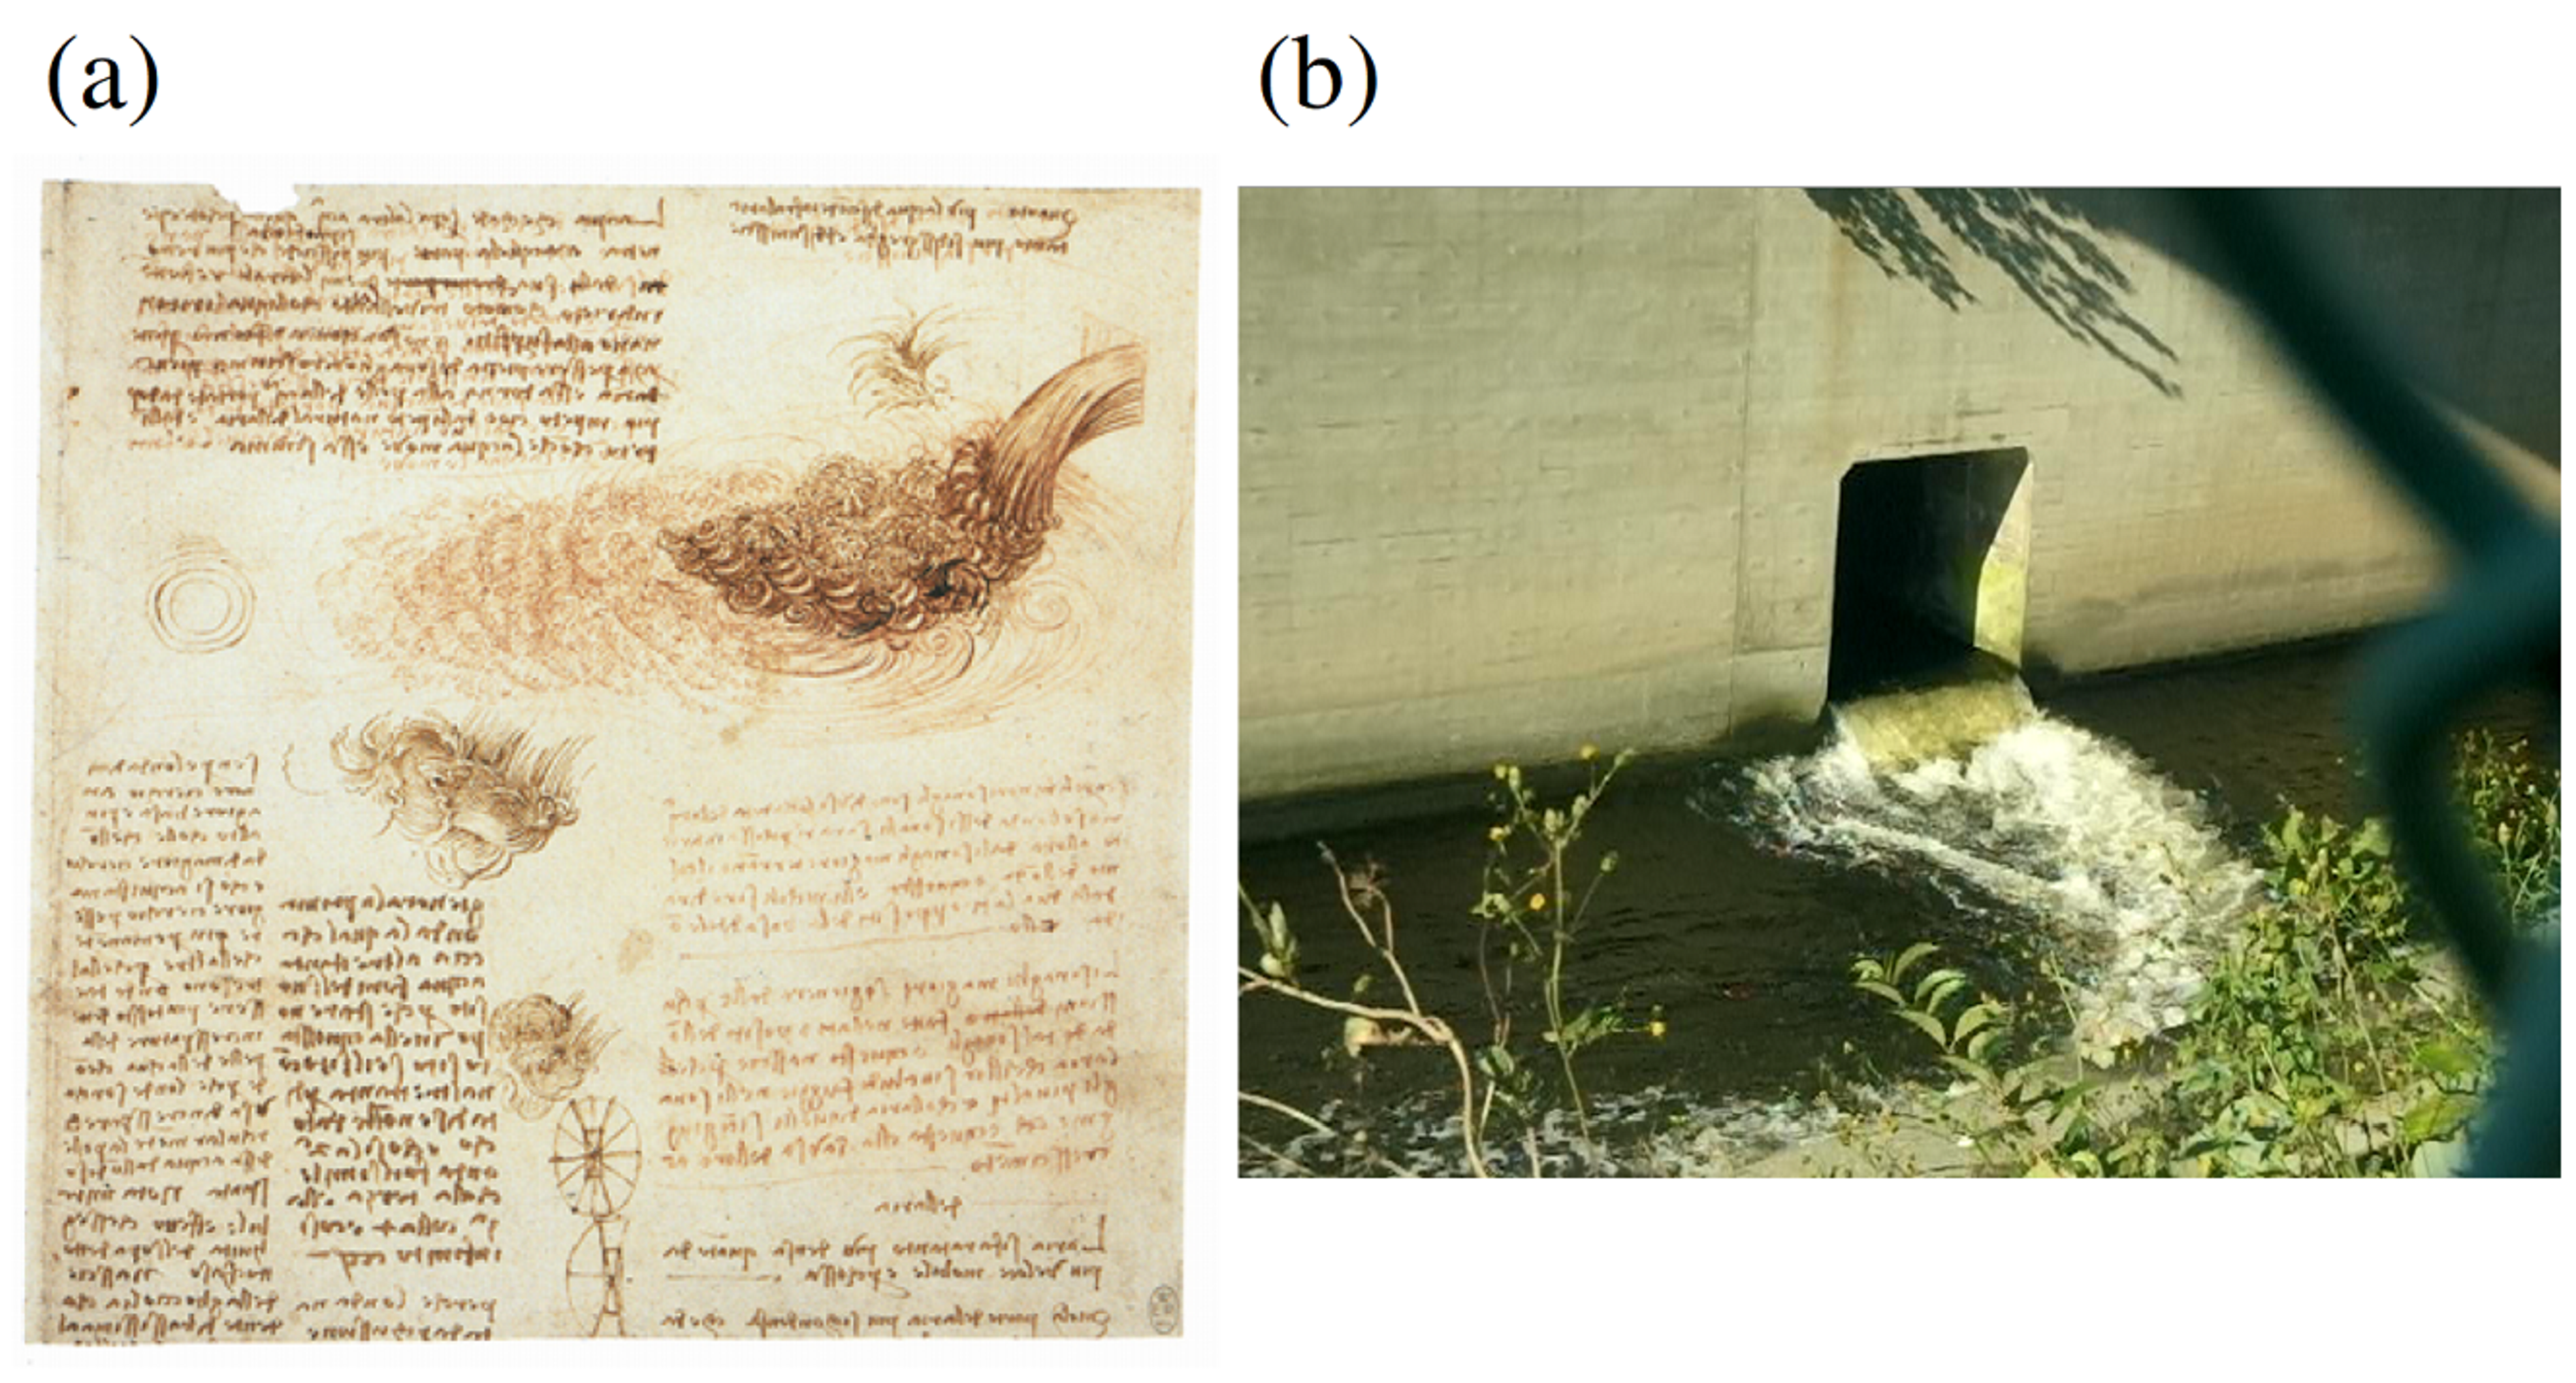
\includegraphics[width=15cm]{galileo.eps}
			\caption{
			(a)はガリレオ・ガリレイがスケッチした乱流の絵画。
            排水溝から排出される大スケールの水流が、水路に流れ出るときに乱流を作り出している様子が描かれている。
            "Turbolenza", The ‘blob’ drawings of Leonardo Da Vinci, Italy, (1508),
            https://lebbeuswoods.wordpress.com/2010/12/03/da-vincis-blobs/
            (b)は多摩川をまたぐ稲城大橋にある北多摩一号水門裏の排水溝。
            条件が同等であれば同じような現象を見ることができる。
			}
			\label{FIG:galileo}
		\end{figure}
        例として図.~\ref{FIG:vorticity}に超流動体における定常乱流を示す。
        $(x,y)=(L,L), L=64$の二次元空間の周期的境界条件を課した系に対して、
        規格化した$\int d^2 \Vec{r} |\psi(\Vec{r})|^2=1$の一様な初期状態から、
        およそ$L/4$のサイズのランダムポテンシャルによるエネルギーを注入し
        流体の運動エネルギーが定常になるまで十分な時間が経過した状態である。
        (a)は密度分布を示し、乱流により乱雑な状態であることがわかる。
        (b)は同じ時刻の速度場を示し、速度ベクトルで可視化すると
        乱雑な分布から、大小の流れや渦が見えてくる。
        そして密度分布からより定量的な速度の情報を得ることでエネルギーの分析が可能となる。
        ランダムポテンシャルの詳細については~\ref{s:random}(B)にて示す。
		\begin{figure}[H]
			\centering
			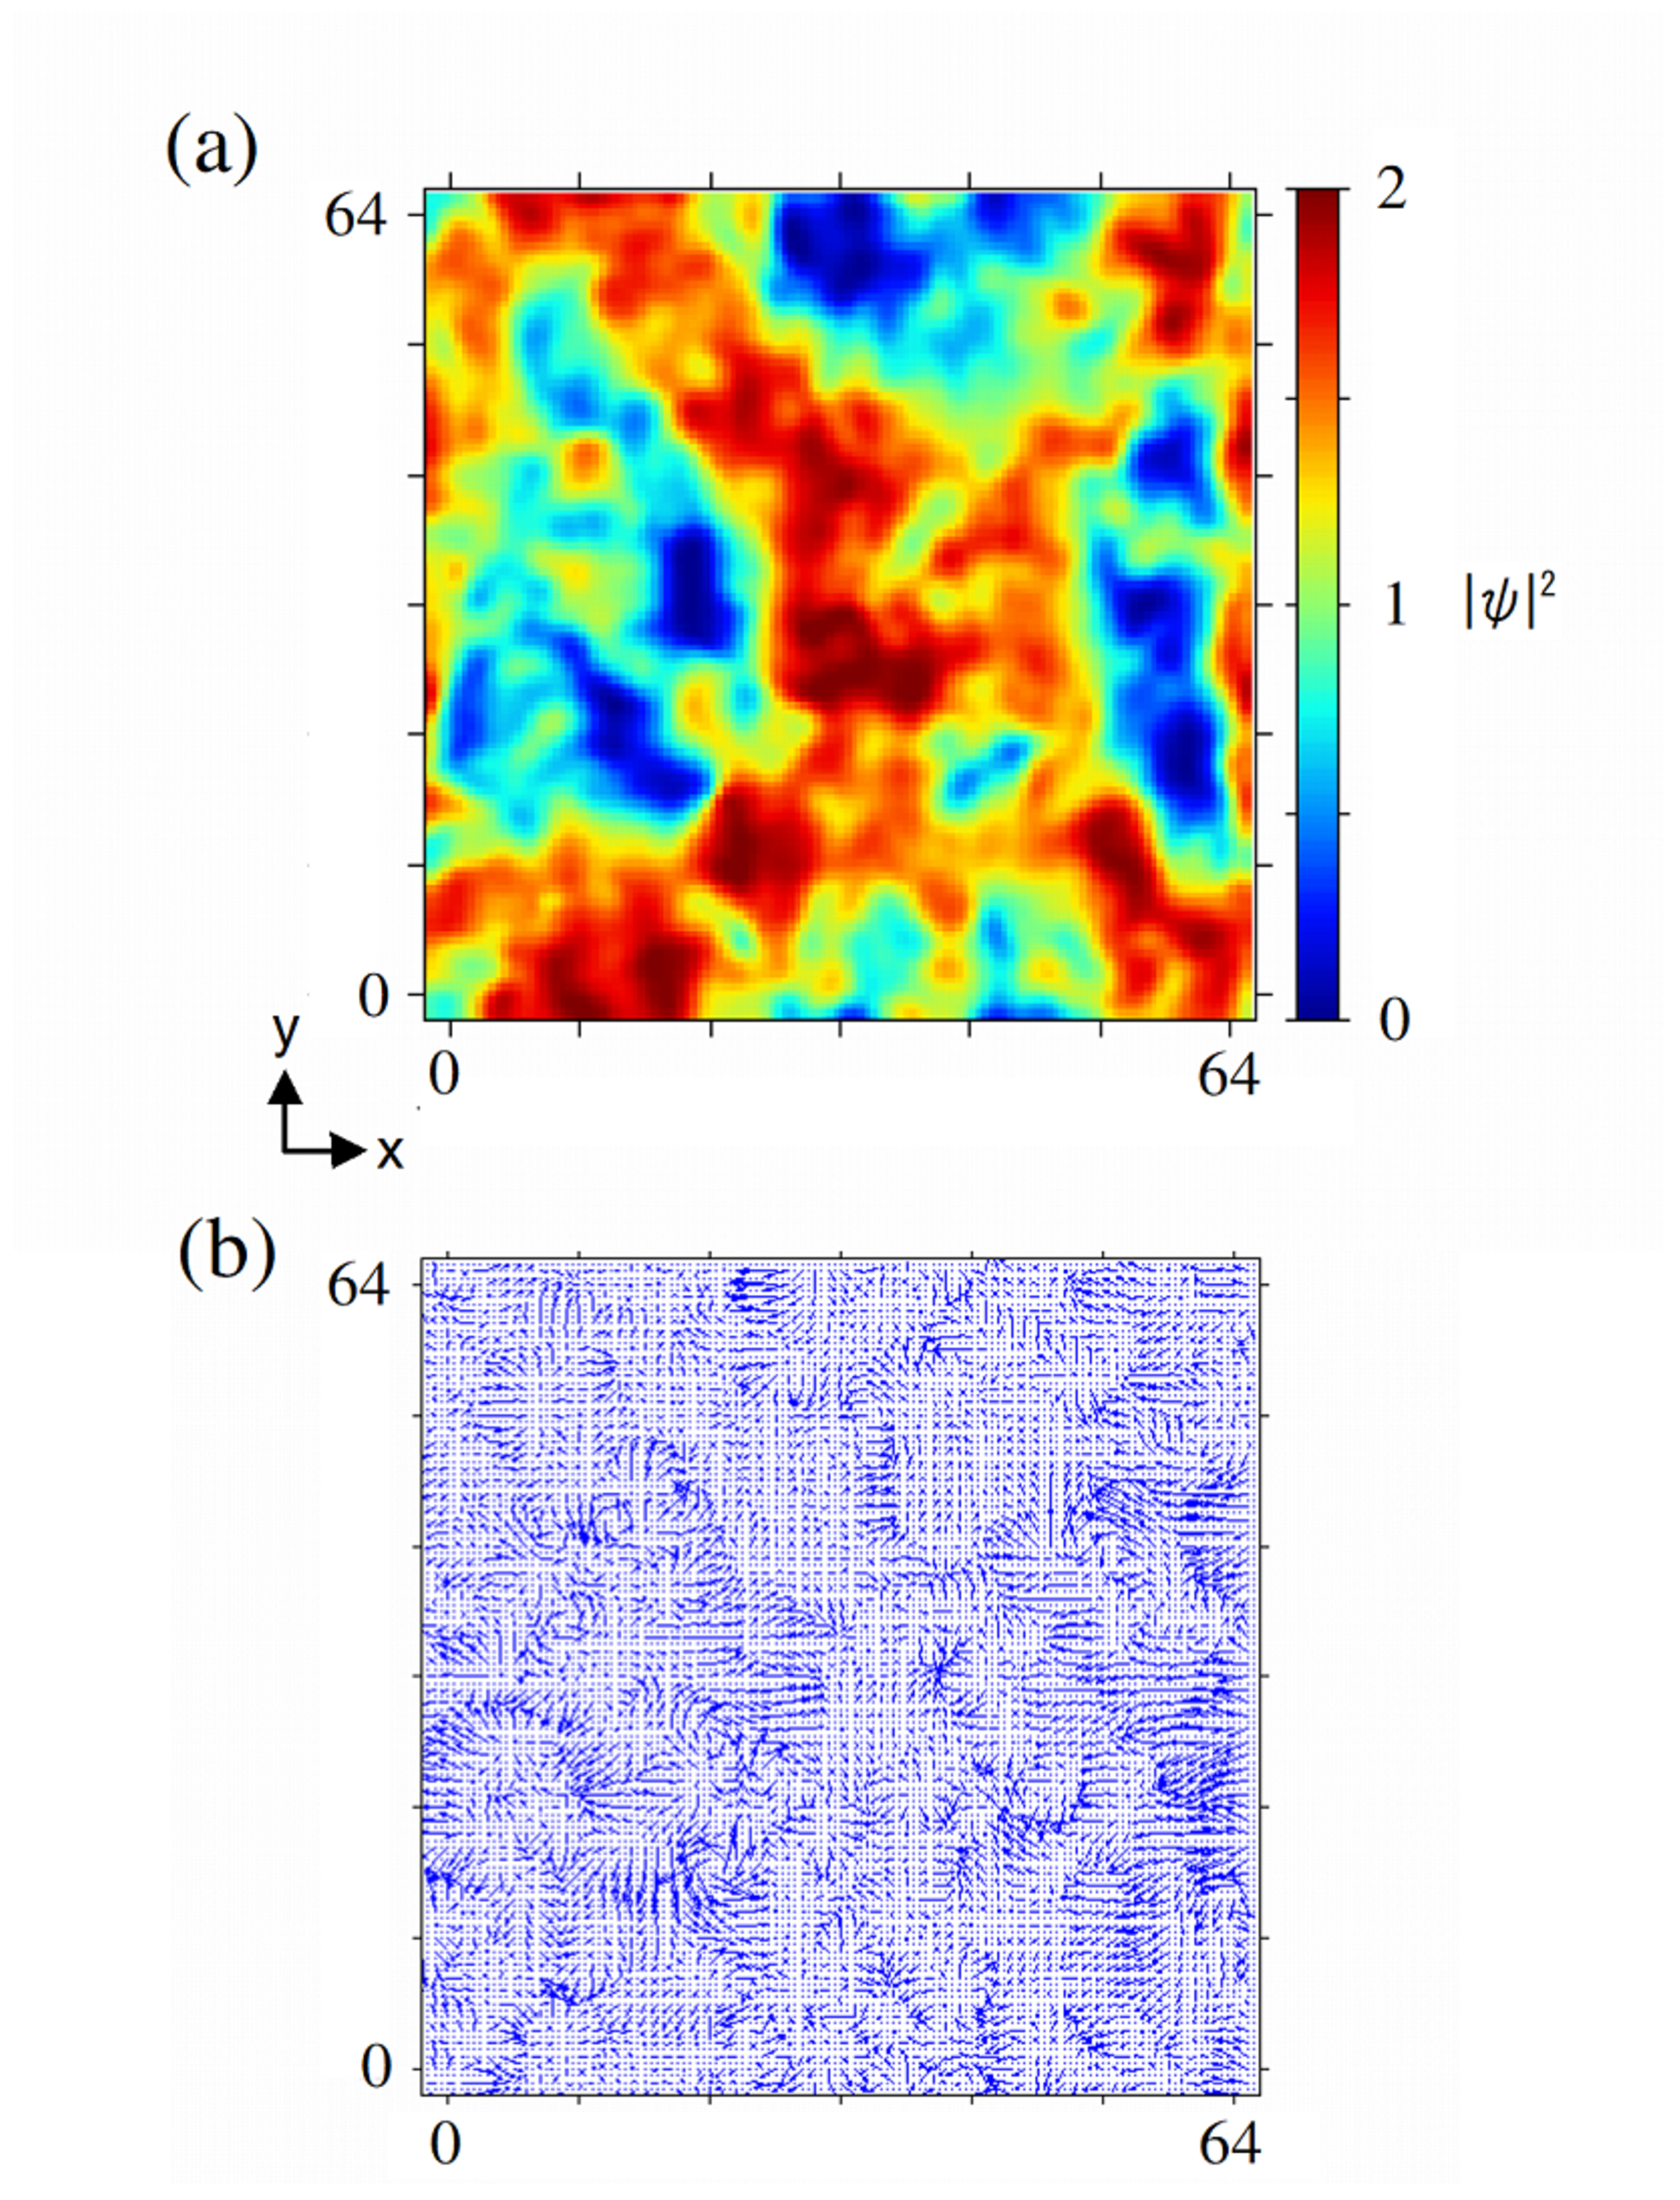
\includegraphics[width=14cm]{vorticity.eps}
			\caption{
                (a)は定常乱流の確率密度$|\psi|^2$、(b)は同じ時刻の速度場のベクトル図。
                $(x,y)=(L,L), L=64$の二次元空間の周期的境界条件を課した系に対して、
                およそ$L/4$のサイズのランダムポテンシャルによるエネルギーを注入し
                流体の運動エネルギーが定常になるまで十分な時間が経過した状態である。
                定常状態の乱流中では大小のスケールの渦や流れが見られる。
                数値計算は擬スペクトル法を用いて算出した。
                数値計算の詳細については~\ref{s:numeric}(A)にて示す。
			}
			\label{FIG:vorticity}
		\end{figure}
        乱流研究は他の物理と同じく、一見すると複雑な様子または見逃がしてしまう様子から、
        速度やエネルギーなど定量的な情報を得ることで
        規則性や法則を見出すことである。
		ここでは本研究に関連する古典乱流と量子乱流の先行研究についてレビューをする。


		\section{古典流体における乱流研究}
		古典流体では、乱流状態の指標としてレイノルズ数${\textrm Re}$を用いて、
		多くの実験結果で${\textrm Re} > 2000$の範囲で得られている~\cite{Reynolds,Goto2}。
		実験研究や工学技術ではレイノルズの相似法則をモデルにして、広範囲な物体のスケールや流体の種類で実用化されている。
		レイノルズ数は流体の運動方程式、ナビエ・ストークス方程式
		$\frac{\partial u}{\partial t} + (v \cdot \nabla) v = -\frac{1}{\rho}\nabla p + \nu \nabla^2 v$の慣性項と
		粘性項の比(${\textrm Re} \equiv \frac{(v \cdot \nabla)v}{\nu \nabla^2 v}=\frac{v l}{\nu}$)の無次元量で定義される。
        $v, t, \rho, p, \nu$はそれぞれ流体の速度場、時刻、流体の密度、圧力、動粘性率である。
		${\textrm Re} > 2000$の乱流状態では分母の粘性項よりも分子にくる慣性項が支配的となる。
		慣性項の$(v \cdot \nabla) v$について一次元のモデルを想定すると、
		乱流状態の流体速度の変動を$v(x)=v^\prime \cos(kx)$、波数空間を$k$、実空間を$x$と仮定したとき、
		\begin{eqnarray}
			(v \cdot \nabla) v = v^\prime \cos(kx) \cdot \frac{\partial v^\prime \cos(kx)}{\partial x}
			= -v^{\prime2} k \cos (kx) \sin (kx) = -v^{\prime2} k \sin (2kx),
		\end{eqnarray}
		と記述され、慣性項が支配的となる場合では任意の大きさの渦から、
        $2$倍の高波数スケールの力が流体中で積極的に作用し半分のスケールの渦が生成される。
		このはたらきによって、乱流中において低波数スケールの乱れが
		高波数スケールの乱れに分裂、カスケードしていくと試算できる~\cite{Tatsumi2}。
		可視的には、乱流中で起きる大きな渦が、小さな渦へと漸化的に分裂していく過程を、
        気象学者のリチャードソンが記録を残し、
		リチャードソン・カスケードとして知られている~\cite{Richardson}。
        図.~\ref{FIG:spectrum}(a)はその慣性領域で渦が分裂していく過程のイメージである。
        定常に発達した乱流では大きいスケールの流体の要素が、周囲の速度や
        要素自身の流れの不安定性によって渦巻き、次第に
        小さな流体要素へと分裂し最終的には分裂のエネルギーが散逸する。
        古典乱流の散逸では粘性による熱に変換される。
        この過程をエネルギーカスケードという。
        乱流ではレイノルズ数$\textrm{Re}=(v l)/\nu$、($l$はシステムサイズ)が非常に大きいため、
        分母にあらわれる粘性に依らなくなる。
        図.~\ref{FIG:spectrum}(b)は横軸が波数$k$、縦軸がエネルギースペクトル$E(k)$を
        あらわすグラフである。乱流状態のエネルギースペクトルは波数に対して
        $-5/3$のべき乗に従うエネルギースペクトルを示す慣性領域(${\rm Ef}(k)$)がありその前後の
        低波数側($\rm{ki}$)ではエネルギー注入し、高波数($\rm{kd}$)でエネルギー散逸する。
        %流体要素がスケール間でエネルギーを輸送する範囲を慣性領域といい、
        %図.~\ref{FIG:spectrum}(b)が示すように慣性領域よりも低波数でエネルギーが注入され、
        %高波数でエネルギーが散逸される。
        %乱流中における慣性領域のスケール間で輸送される平均エネルギー$\langle |\delta \Vec{u}(\Vec{r})|^2 \rangle$は、
        %粘性によらずエネルギー注入率$\epsilon$と各スケール$r$が支配的となる仮定から表~\ref{table:dimension}の次元解析を用いて、
        %\begin{table}[H]
        %    \caption{次元解析}
        %    \label{table:dimension}
        %    \centering
        %    \begin{tabular}{lcr}
        %        \hline
        %        & 物理量 & 次元 
        %        \\
        %        \hline \hline
        %        平均エネルギー & $\langle | \delta \Vec{u}(\Vec{r})|^2 \rangle$  & $[L^2 T^{-2}]$
        %        \\
        %        エネルギー注入率 & $\epsilon$ & $[L^2 T^{-3}]$
        %        \\
        %        スケール & $r$ & $[L^1]$
        %        \\
        %        平均エネルギーを $\epsilon$ と $r$ であらわす & $(\epsilon r)^{2/3}$ & $[L^2 T^{-3} L^1]^{2/3} = [L^2 T^{-2}]$
        %        \\
        %        \hline
        %    \end{tabular}
        %\end{table}
        %から、
        %\begin{eqnarray}
        %    \label{eq:cvelocity}
        %    %\langle | \delta \Vec{u}(\Vec{r})|^2 \rangle & : & [L^2 T^{-2}], \nonumber
        %    %\\
        %    %\epsilon & : & [L^2 T^{-3}], \nonumber
        %    %\\
        %    %r & : & [L^1], \nonumber
        %    %\\
        %    %(\epsilon r)^{2/3} & : & [L^2 T^{-3} L^1]^{2/3} = [L^2 T^{-2}], \nonumber
        %    %\\
        %    \langle | \delta \Vec{u}(\Vec{r})|^2 \rangle
        %    & = & \langle
        %        |\Vec{u}(\Vec{x}+\Vec{r})-\Vec{u}(\Vec{x})|^2
        %    \rangle
        %    = C (\epsilon r)^{2/3},
        %\end{eqnarray}
        %の速度相関の関係式であらわされる。$C$は任意定数である。
        %エネルギースペクトルについては、フーリエ変換を用いて波数空間での表現に置き換え、
        %\begin{eqnarray}
        %    E(k) = C^\prime \epsilon^{2/3} k^{-5/3},
        %\end{eqnarray}
        %で得られ、コルモゴロフの$-5/3$べき乗則という。
        % %図.~\ref{FIG:spectrum}(a)では、
        % %リチャードソンがスケッチした大きいスケールの渦から次第に小さなスケールの渦に分裂する様子のイメージ~\cite{Richardson}。
        %図.~\ref{FIG:spectrum}(b)では、
        %慣性領域のスケール間の平均エネルギーが高波数へカスケードする様子の対応を示す。
        以上のように複雑と思われる乱流の現象について、エネルギーの側面から定量的な情報を得られることを足掛かりに、
        本研究では量子乱流のエネルギーカスケードについて古典乱流の研究と照らし合わせて調査を進めた。
        \begin{figure}[H]
            \centering
            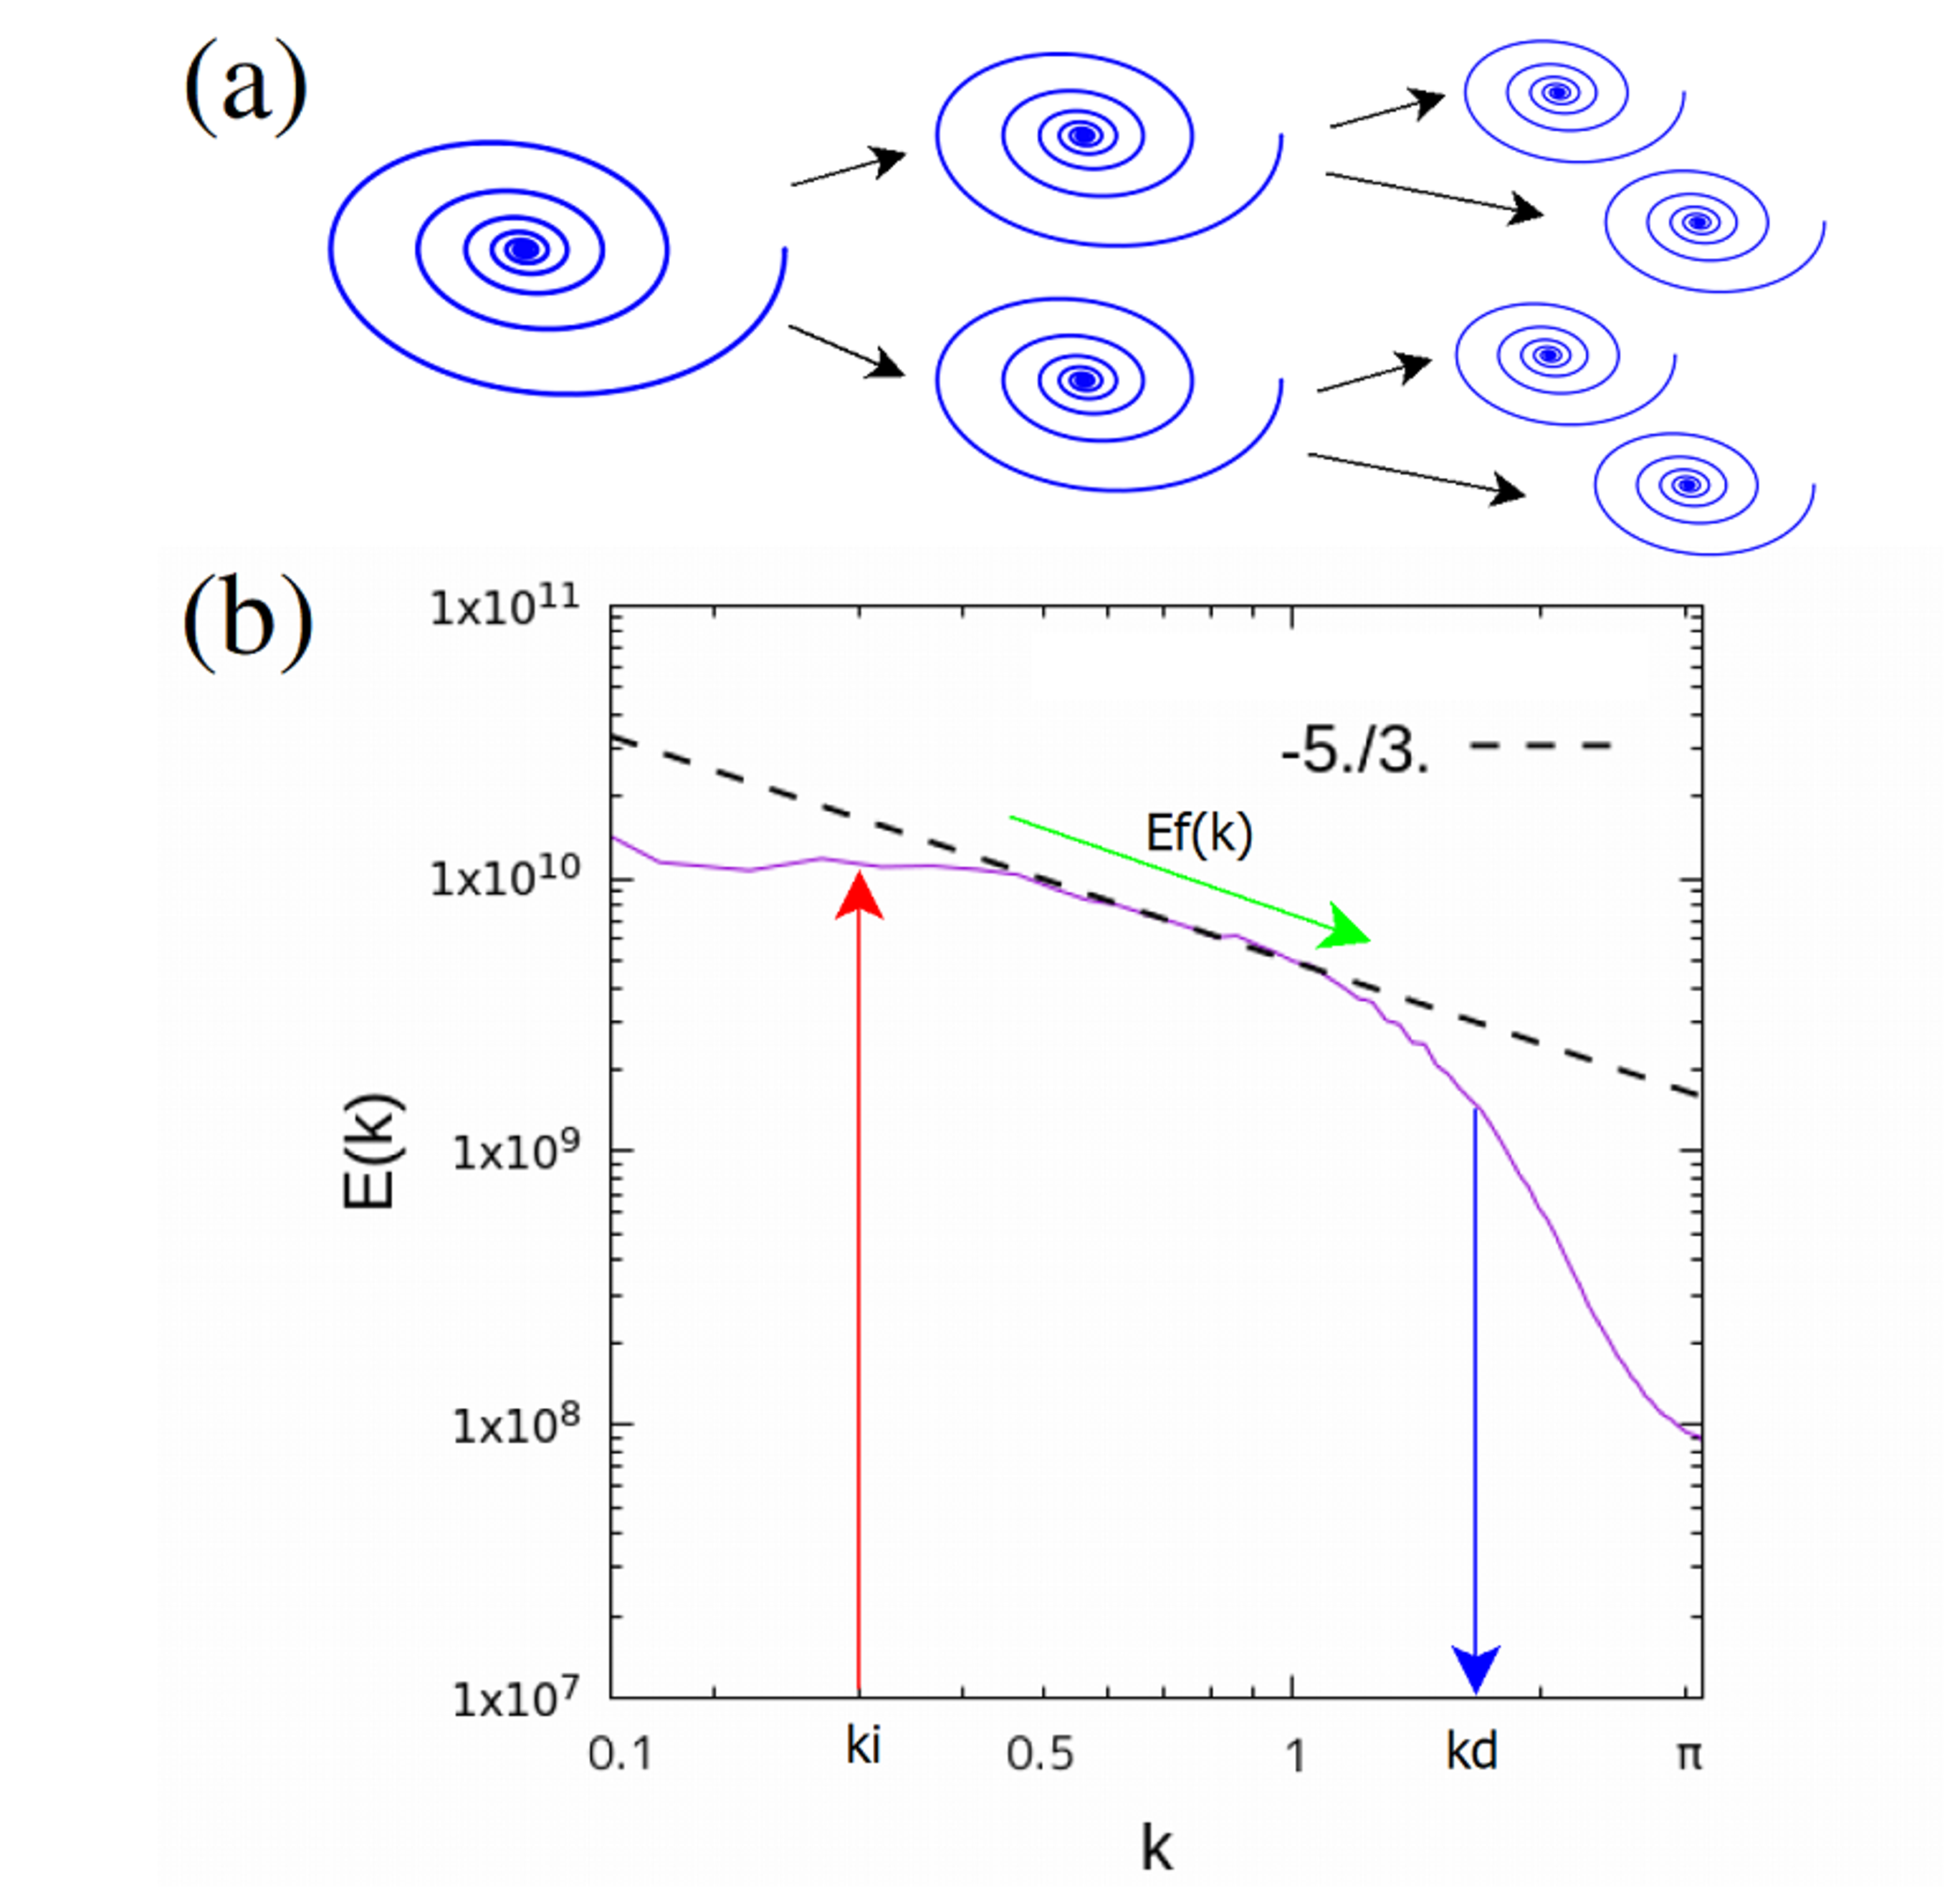
\includegraphics[width=15cm]{spectrum.eps}
            \caption{
                (a)は乱流状態の慣性領域における大スケールの渦が小スケールの渦へカスケード分裂するイメージ図。
                (b)はの乱流の系のエネルギースペクトル$E(k)$を示す。
                (a)のイメージで描くような渦の分裂がエネルギースペクトルの慣性領域で起きている。
                低波数領域${\rm ki}$(induction)でエネルギーが注入され、
                乱流の慣性領域${\rm Ef}(k)$(energy flux)ではエネルギーがカスケードし、
                高波数領域$\rm{kd}$(dissipation)でエネルギーが散逸される。
                得られたグラフの系は
                $128^3$の三次元で超流動体が定常乱流に達している全空間のエネルギーから算出した。
                詳細は本論文の~\ref{s:distributions}節を参照。
            }
            \label{FIG:spectrum}
        \end{figure}


        \section{コルモゴロフ理論}
        コルモゴロフは乱流において支配的となる物理量を推察し、十分大きな流体の系で
        発達した乱流の現象があらわている小さな区画に着目した。
        この区画の乱流は一様で等方的であり、十分に大きな系が乱流をもたらすメカニズムの詳細によらない普遍的な物理量であると考え、
        二つの仮説を立てた~\cite{Kolmogorov}。
        一つ目の仮説はこの区画の一様で等方的な乱流で
        支配的な物理量は、システムサイズ$l$と、
        エネルギーが注入から高波数のスケールへカスケード伝搬するときの平均的なエネルギーレート$\epsilon$、
        そしてエネルギーが熱散逸する際にはたらく動粘性率$\nu$であるとした。
        これらの物理量であらわした空間$\eta$、時間$\tau_\eta$、速度$v_\eta$、流体密度$\rho_\eta=1$、
        エネルギーレート$\epsilon=\langle (\rho_\eta v_\eta^2)/\tau_\eta \rangle$は
        \begin{eqnarray}
            \eta & = & \left( \nu^3 / \epsilon
            \right)^{1/4} \nonumber
            \\
            \tau_\eta & = & (\epsilon \nu)^{1/4} \nonumber
            \\
            v_\eta & = & (\nu / \epsilon)^{1/2}
        \end{eqnarray}
        で示される。
        また、この単位系のレイノルズ数、
        \begin{eqnarray}
            \textrm{Re}_{\eta} = \frac{v_{\eta} \eta}{\nu} = 1
        \end{eqnarray}
        が得られる。
        レイノルズ数は$1$となり慣性力と粘性力の比がつりあう。
        発達した乱流ではレイノルズ数が$1$よりも十分大きな値であることから、
        これらの関係は乱流における最も小さなスケールをあらわしている。
        この単位系の運動エネルギーは、
        \begin{eqnarray}
            E(k) \propto  v_\eta^2 \eta,
        \end{eqnarray}
        で示される。
        これを$\nu, \epsilon$と波数$k=\eta^{-1}$の物理量であらわすと、
        \begin{eqnarray}
            v_\eta^2 \eta = \epsilon^{1/4} \nu^{5/4} (k / \eta^{-1})^n = \epsilon^{1/4} \nu^{5/4} (k \epsilon^{-1/4} \nu^{3/4})^n
        \end{eqnarray}
        を得る。$(k \epsilon^{-1/4} \nu^{3/4})^n$は無次元量の$n$乗で括られる。
       
        二つ目の仮説は、レイノルズ数が大きな値を示す乱流の慣性領域で
        支配的な物理量がシステムサイズ$l$と平均的なエネルギーレート$\epsilon$によって
        決定され、動粘性率$\nu$に依らない。
        このことから、$\nu$に依らない無次元量$(k \epsilon^{-1/4} \nu^{3/4})^{n=-5/3}$が要請され、
        この仮説より運動エネルギーは、
        \begin{eqnarray}
            E(k) = C \epsilon^{2/3} k^{-5/3}
        \end{eqnarray}
        を得る。$C$は任意定数である。
        これをコルモゴロフの$-5/3$べき乗則といい、多くの実験、数値計算で確認されている
		~\cite{Frisch1, Kolmogorov, Batchelor, Tatsumi1, Tatsumi2, Kraichnan, Frisch2, Cyril, Goto1, Goto2}。
        例として図.~\ref{FIG:spectrum}(b)では、に乱流の系のエネルギースペクトルを示す。
        流体要素が乱流中のスケール間でエネルギーを輸送する範囲$E\rm{f}(k)$を慣性領域といい、
        慣性領域よりも低波数$\rm{ki}$でエネルギーが注入され、高波数$\rm{kd}$で散逸される。


		\section{渦度の可視化によるエネルギーカスケードの考察}
        \label{s:orth}
		古典乱流におけるエネルギーカスケードについて後藤らは乱流中の渦バンドルの可視化に着目し、リチャードソンが描くような
        低波数渦度から高波数渦度へカスケードする構造があることを調査発見した~\cite{Goto1,Goto2,Goto3,butsuri1}。
		特徴的な発見として、低波数の渦バンドルから高波数の渦バンドルが生成されるとき、直交した配置をとることが確認された。
		この直交性の定量的な分析に、低圧力法を用いて渦バンドル断面の圧力勾配の極小値をつなぎ合わせた渦中心の構造を得る。
		大小渦スケールのカスケード過程を、それぞれの渦中心の配置から角度関係を相関関数を用いて算出した。
		分析の結果から、低波数から高波数へ渦バンドルがカスケード生成する際、その構成は定量的に直交性を示していることがわかった。
        図.~\ref{FIG:cortho}の例では、(a)に示す大スケールの渦度$W_1$から、小スケールの渦度$W_2$が
        直交に生成され、その配置の角度分布についての分析結果も(b)のように直交であることを示している。
		\begin{figure}[H]
			\centering
			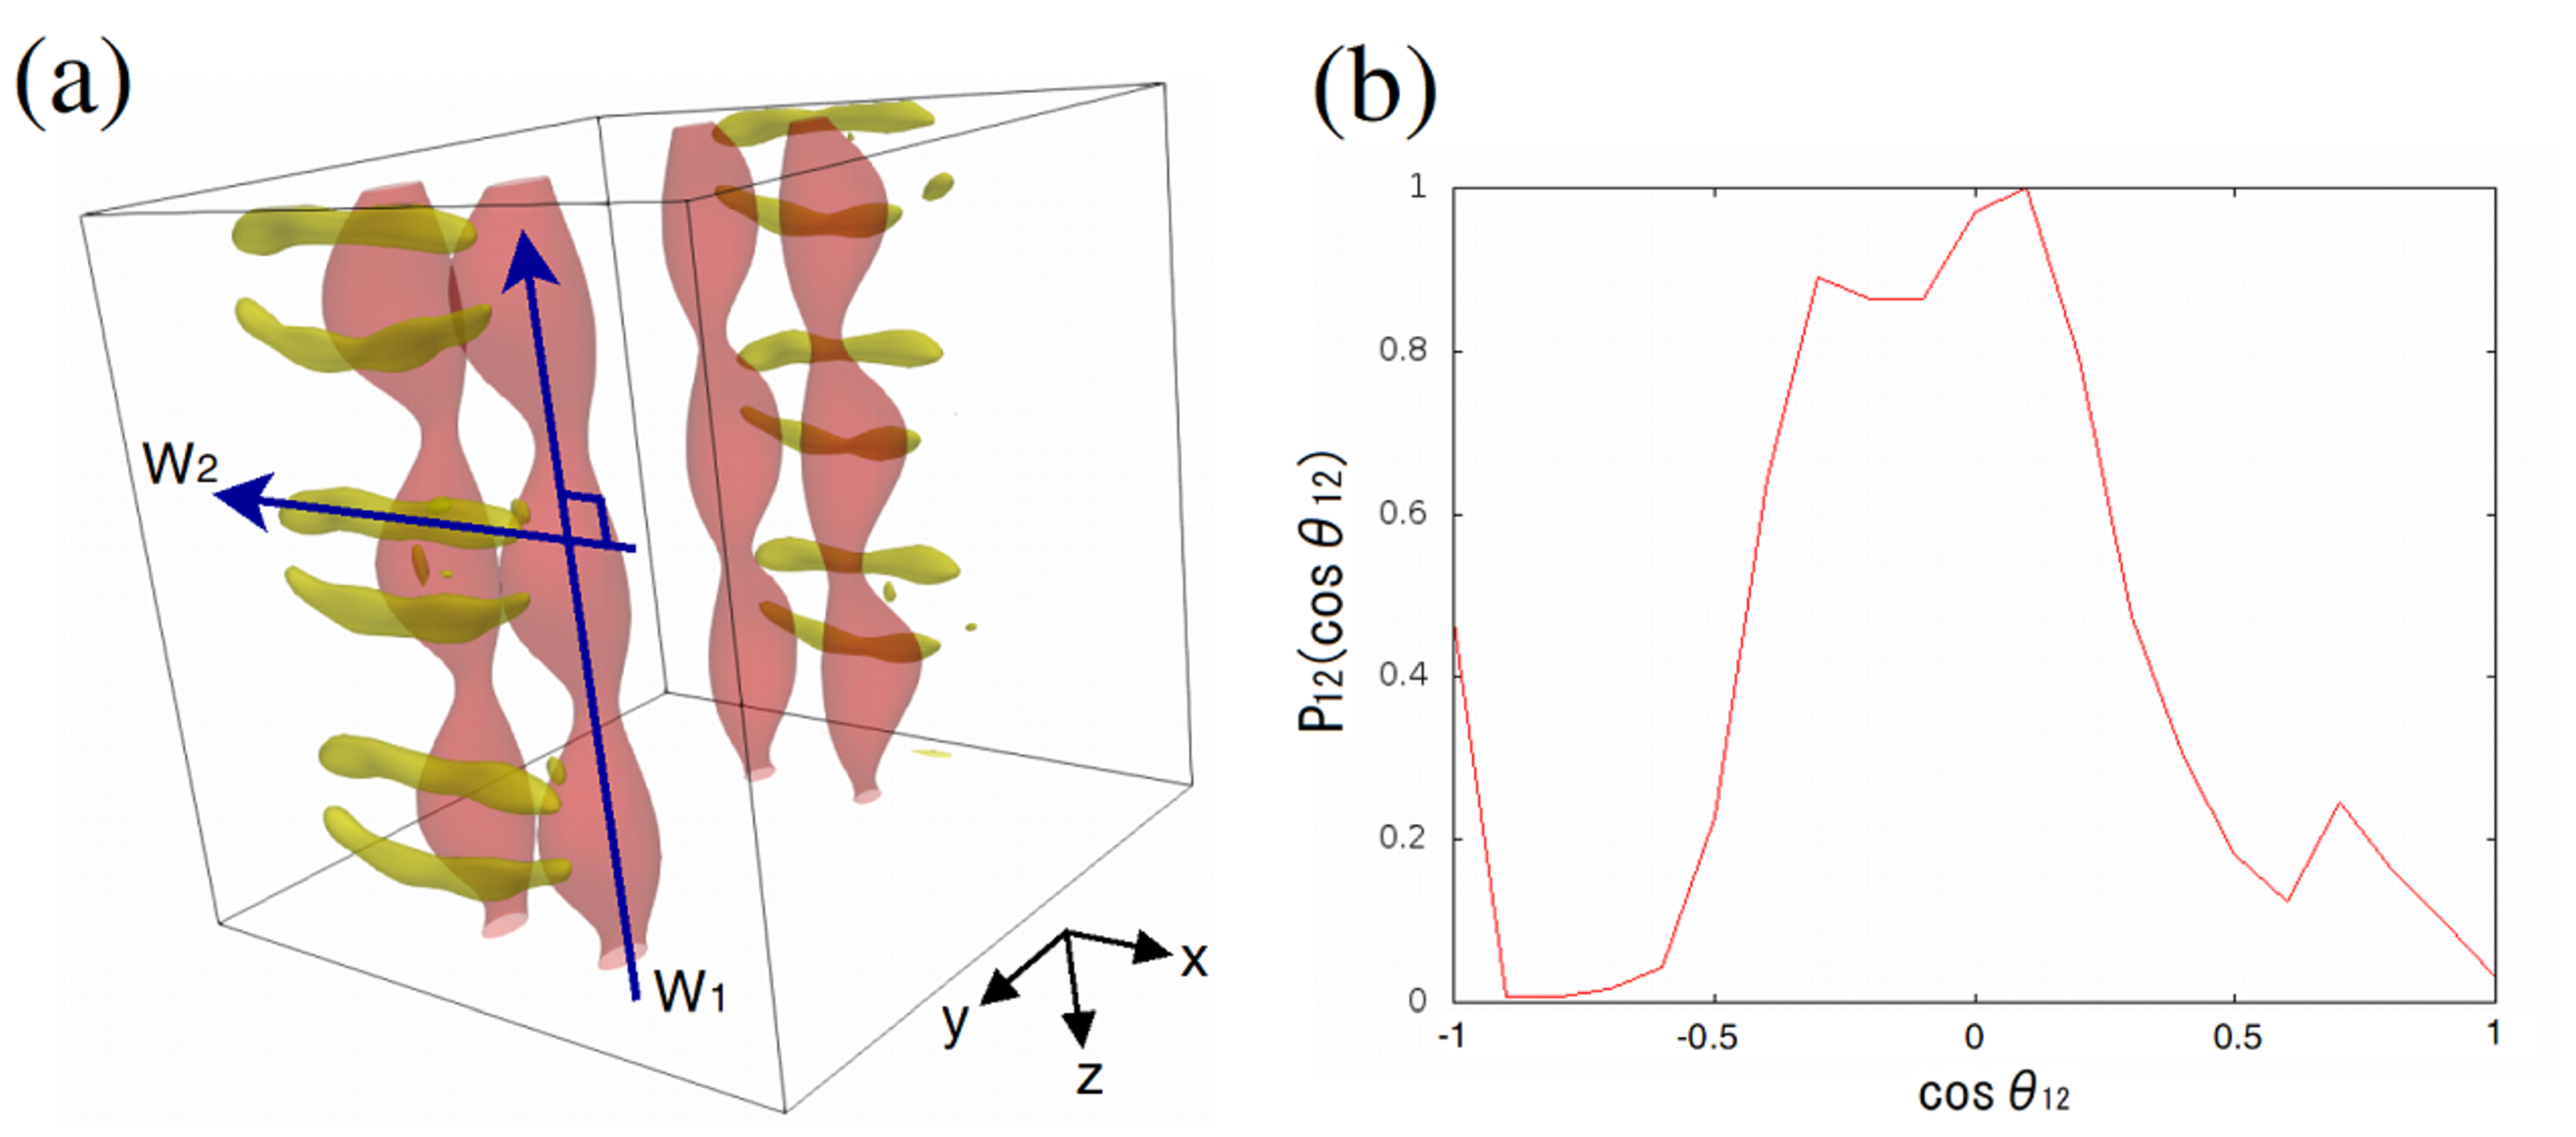
\includegraphics[width=15cm]{cortho.eps}
			\caption{
                (a)は大スケールの渦度$W_1$から小スケールの渦度$W_2$が生成された様子。
                矢印は渦度の回転の向き(右手系)をあらわす。
                (b)は(a)で得られた渦度の$W_1$と$W_2$の間の角度分布を算出。
                相関関数$\cos \theta_{12}=0$にピークがあることから$W_1$と$W_2$の配置される関係が直交性であることがわかる。
                詳細は本論文の~\ref{c:orth}章を参照。
			}
			\label{FIG:cortho}
		\end{figure}
		本研究では超流動体を対象に同様の分析を行い、低波数の渦バンドル配置からの調査に加え、
        発達した等方乱流に対しても同様の分析を進め、量子乱流における渦度の階層構造を調査した。
		量子流体では位相欠陥による量子渦構造が存在するため、
		大スケールの渦バンドルから小スケールへカスケードしていく具体的な様子を抽出することができる。


		\section{二流体乱流におけるエネルギー注入率と流滴サイズ}
		水と油のような互いに溶け合わない分離した二流体に対して、
        ドレッシングを混ぜる要領で外部からエネルギーを注入すると、
        乱流が発生し水と油は細かな流滴に分裂した状態で入り混じる。
        そして外部のエネルギーの大小と分裂する流滴サイズの関係は一意的に対応する。
        エネルギーが大きい場合では、流滴が大きなサイズで維持することができず、
        比較的細かく分裂する。エネルギーが小さい場合では分裂するための力が弱く
        細かく分裂しにくい。そしてエネルギーをなくしてしまうと次第に同じ成分どうしがまとまっていき、
        二流体は再びそれぞれ一つの大きな領域に分離する。


        コルモゴロフとヒンゼは
        この二流体乱流においてウェーバー数から、外力のエネルギー注入率と流滴サイズの関係性を
		導いた~\cite{Kolmogorov49,Hinze}。
        ウェーバー数${\mathrm We}$は無次元数、
        \begin{eqnarray}
            \label{eq:weber}
            {\mathrm We} = \frac{\rho \langle u^2 \rangle D}{\sigma},
        \end{eqnarray}
        であらわされる。
        $\rho, u, D, \sigma$は、それぞれ流体の密度、速度、流滴サイズ、表面張力を示す。
        流体速度の二乗平均$\langle u^2 \rangle$と、
        乱流中における支配的な物理量のエネルギー注入率$\epsilon$と流滴サイズ$D$それぞれの次元について、
        \begin{table}[H]
            \caption{次元解析}
            \label{table:khdimension}
            \centering
            \begin{tabular}{lcr}
                \hline
                & 物理量 & 次元 
                \\
                \hline \hline
                流体速度の二乗平均 & $\langle u^2 \rangle$  & $[L^2 T^{-2}]$
                \\
                エネルギー注入率 & $\epsilon$ & $[L^2 T^{-3}]$
                \\
                流滴サイズ & $D$ & $[L^1]$
                \\
                $\langle u^2 \rangle$の次元を $\epsilon$ と $D$ であらわす & $C(\epsilon D)^{2/3}$ & $[L^2 T^{-3} L^1]^{2/3} = [L^2 T^{-2}]$
                \\
                \hline
            \end{tabular}
        \end{table}
        で示す。$C$は任意定数。表~\ref{table:khdimension}から、
        \begin{eqnarray}
        %    \langle u^2 \rangle = C(\epsilon D)^{2/3}, \nonumber
            \langle u^2 \rangle
            & = & 
            %\langle
            %    |\Vec{u}(\Vec{x}+\Vec{r})-\Vec{u}(\Vec{x})|^2
            %\rangle
            %= 
            C (\epsilon D)^{2/3},
        \end{eqnarray}
        であらわすことができ~(\ref{eq:weber})に代入し、
        \begin{eqnarray}
            {\mathrm We} & = & \frac{\rho \langle u^2 \rangle D}{\sigma},
            \\
            & = & C \frac{\rho \epsilon^{2/3} D^{2/3} D}{\sigma}
            = C \frac{\rho \epsilon^{2/3} D^{5/3}}{\sigma},
            \\
            D^{5/3} & = & \left( \frac{{\mathrm We}}{C}\right) \left( \frac{\sigma}{\rho} \right) \epsilon^{-2/3},
            \\
            D & = & C^\prime \left( \frac{\sigma}{\rho} \right)^{3/5} \epsilon^{-2/5}
            \ , \ C^\prime = \left( \frac{{\mathrm We}}{C} \right)^{-3/5},
        \end{eqnarray}
        から、
        \begin{eqnarray}
            \label{eq:chinze}
            D(\epsilon) & \propto & \left( \frac{\sigma}{\rho} \right)^{3/5} \epsilon^{-2/5}
        \end{eqnarray}
        が得られエネルギー注入率$\epsilon$と流滴サイズ$D$の関係をむすびつける、
        古典流体におけるコルモゴロフ・ヒンゼ(KH)スケールを得る。$C^\prime$は任意定数
        KHスケールの詳細については~\ref{c:khscale}章で述べる。


        二成分系の古典乱流の場合のエネルギー注入率に対する流滴サイズの関係性について、
        パレカーらは乱流によって二成分がそれぞれもとの各成分へ分離してしまうのを阻止するはたらきに注目し、
        KHスケール~(\ref{eq:chinze})をもとに
        数値計算を用いて調査した~\cite{Perlekar12, Perlekar14}。
        例として図.~\ref{FIG:perlekar}に、
        二成分超流動体による乱流の時間発展の例でその様子を示す。
        系は$L^3=128^3$の空間で周期的境界条件を課してある。
        図.~\ref{FIG:perlekar}(a)から(d)の場合(without forcing)では、
        ランダムに混ざった状態の二流体に対して
        外部からのエネルギーを与えない状況のため最終的には一つの大きな二流体に分離する。
        図.~\ref{FIG:perlekar}(a$'$)から(d$'$)の場合(with forcing A)では、外部から一定のエネルギーを与える状況により、
        二流体が一定の大きさに分離した状態を維持している。
        図.~\ref{FIG:perlekar}(a$''$)から(d$''$)の場合(with forcing B)では、二流体が分離した初期状態から、
        同じ一定のエネルギーを与え、最終的に図.~\ref{FIG:perlekar}(d$'$)と同じ程度の流滴サイズで乱流の状態を維持する。
        結論として、外部のエネルギーの有り無しまたは大小によって完全に分離した状態から、
        分裂する流滴サイズが一意的に対応する範囲があることがわかる。

		\begin{figure}[H]
			\begin{center}
			\includegraphics[width=16cm]{perlekar.eps}
			\caption{
                エネルギー注入の有無について、初期状態からの時間発展の様子を示す。
                三次元二成分系の$L^3=128^3$の空間で周期的境界条件を課してある。
				(a)--(d)は外部からのエネルギー注入がないため二成分が大きく分離する。
				(a')--(d')はエネルギー注入により定常的な乱流状態となり、一定の流滴サイズを維持する。
				(a'')--(d'')は二成分が分離した状態から同じ強さの外部エネルギーを注入し、
                (d')と同じ流滴サイズで定常的な乱流状態となる。
                詳細は本論文の~\ref{c:khscale}章を参照。
			}
			\label{FIG:perlekar}
			\end{center}
		\end{figure}
        確率密度$|\psi|^2$をフーリエ変換し、スペクトルの分布から
        代表的な流滴サイズのピークを得られる。
        図.~\ref{FIG:perlekar2}(a)は図.~\ref{FIG:perlekar}の定常乱流に到達するまで流滴サイズの時間発展を示す。
        外力がない場合(without forcing)は二成分が分離し、システムサイズで頭打ちになる。
        外力がある場合(with forcing A/B)は、異なる初期状態であっても、同じ外力であれば一定の流滴サイズを維持した状態になる。
        (b)は流滴サイズの頻度分布で、外力がない場合(without forcint)は低波数にピークが分布し、
        外力がある場合(with forcing A/B)は特定のスペクトルにピークがあらわれる。
        このように、確率密度で得られる可視的な情報から流滴サイズを分析することができる。
		\begin{figure}[H]
			\begin{center}
			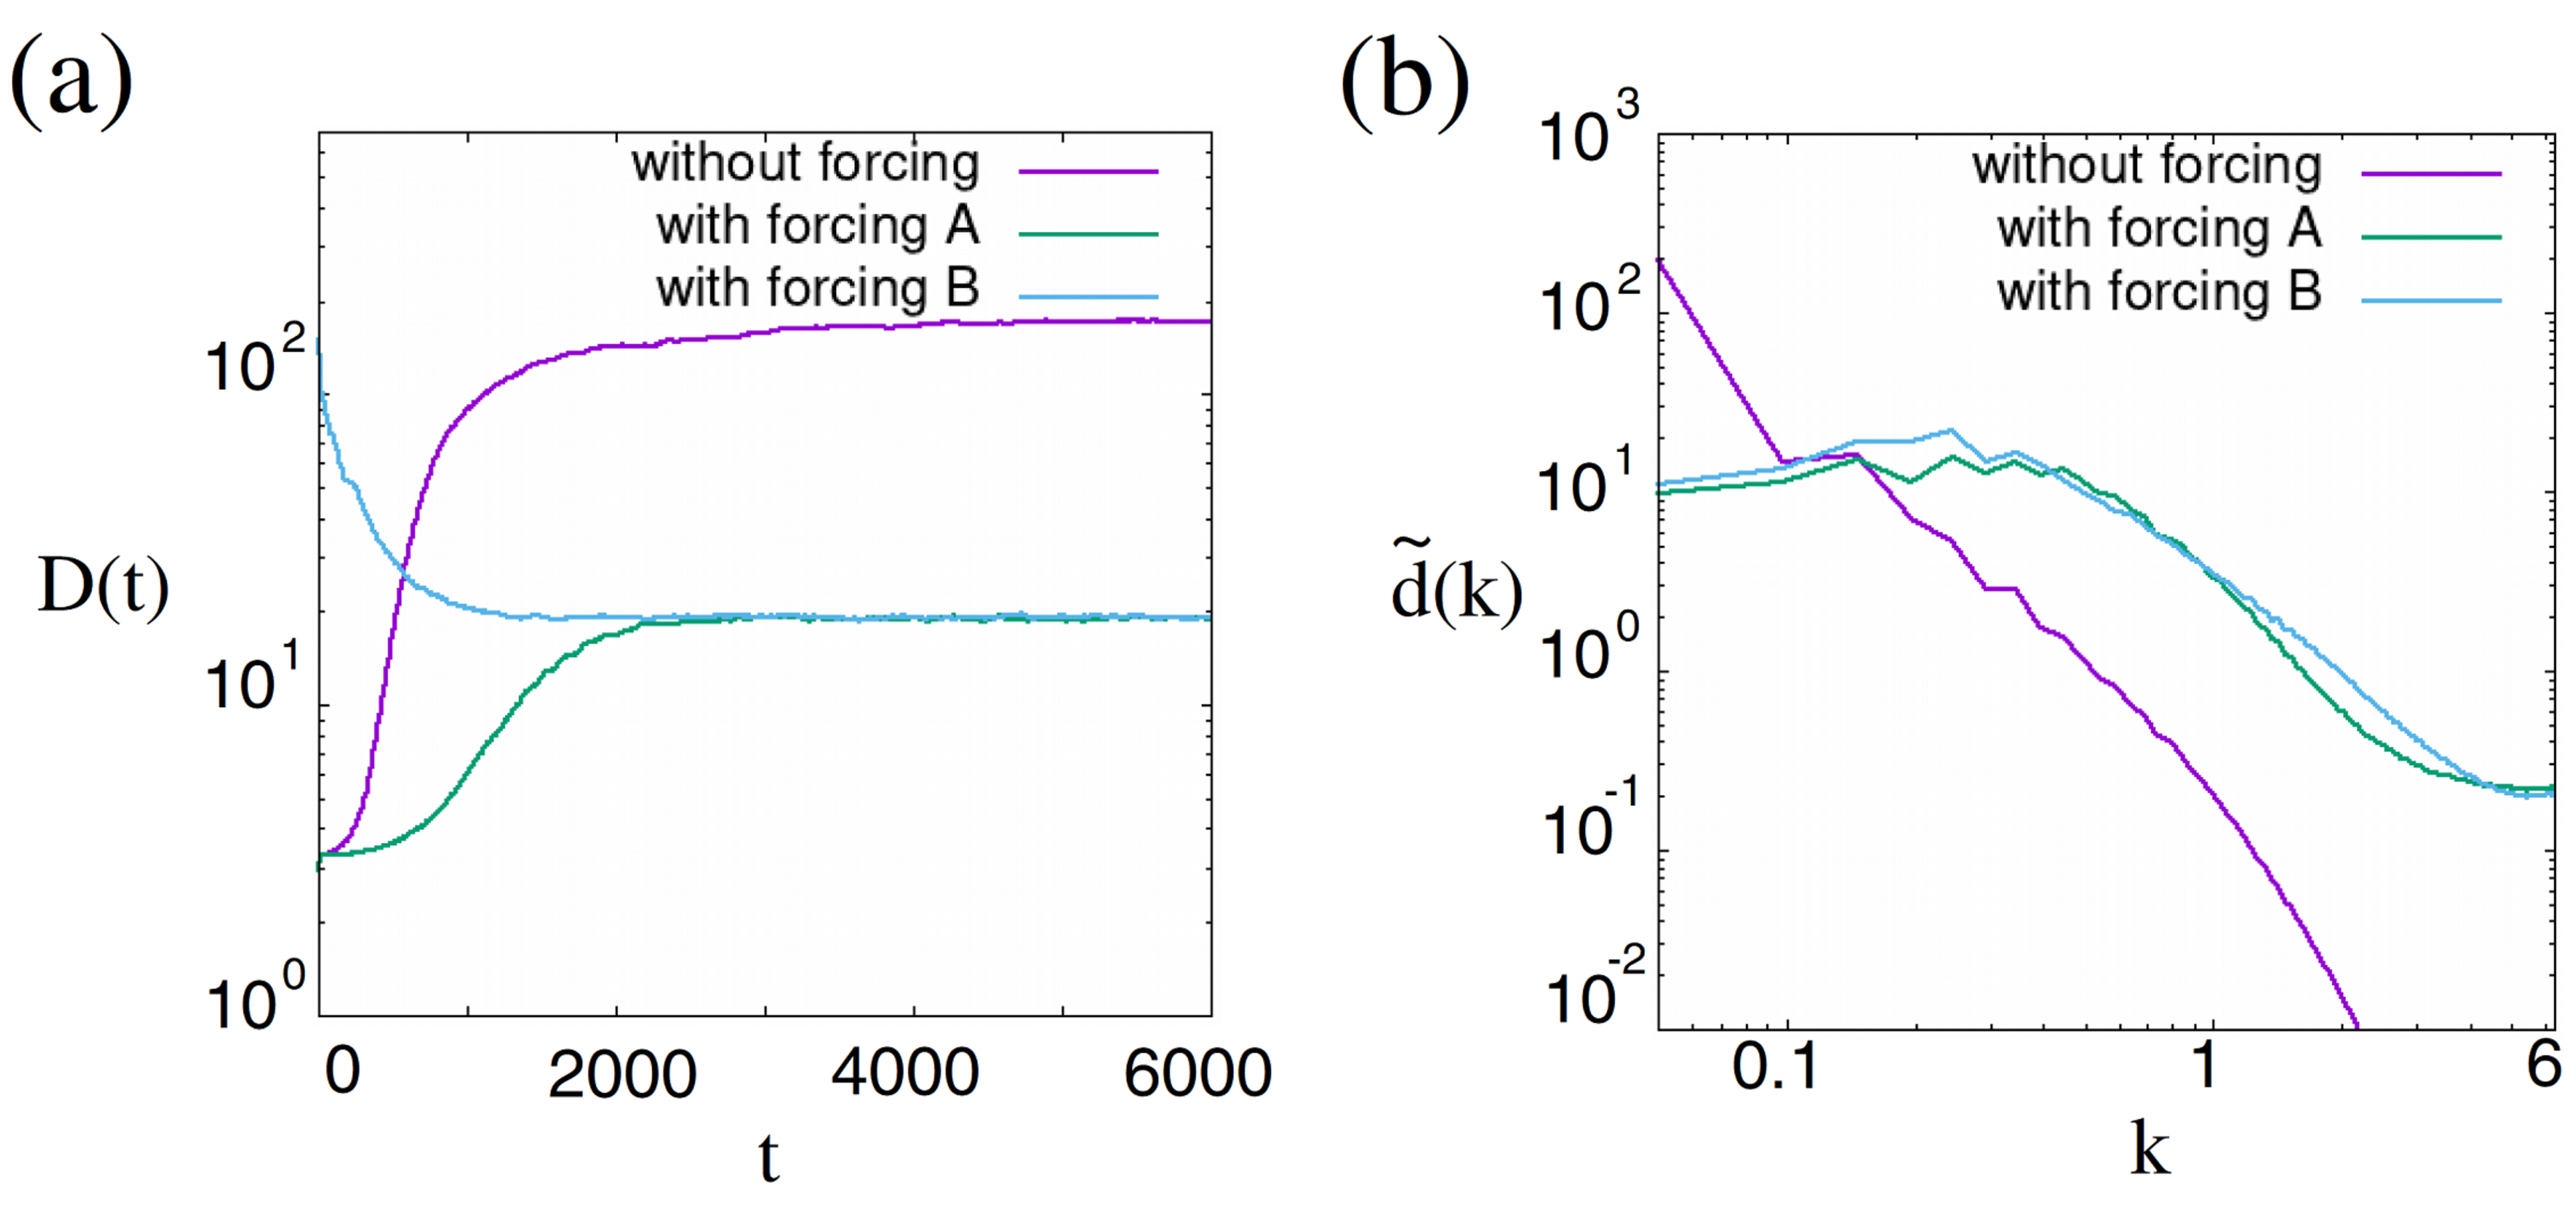
\includegraphics[width=16cm]{perlekar2.eps}
			\caption{
				(a)は図.~\ref{FIG:perlekar}のそれぞれの時間発展を示す。
				(b)は同じく時刻$t=5000$の流滴サイズの出現頻度のスペクトル分布を示す。
                外力がない場合は二成分が大きく分離してしまっているため最低波数にピークがあるが、
                外力がある場合はそれぞれの成分が一定の流滴サイズで分裂しピークの位置が$k=0.3$前後の波数スペクトルに分布する。
			}
			\label{FIG:perlekar2}
			\end{center}
		\end{figure}

		\section{量子流体における乱流研究}
		主な量子乱流の先行研究についての事例を概説する。
        数値計算を用いた理論研究では、
        ノアらはテイラー・グリーン渦の集合体から時間発展させ、
        超流動体による量子乱流を発見した。量子乱流のエネルギースペクトルはコルモゴロフ則を満たしている~\cite{Nore}。
        小林らの超流動体$\rm{^4He}$を想定した三次元量子乱流において、
        慣性領域のエネルギースペクトルは非圧縮性流体の運動エネルギーから、コルモゴロフ則を
        満たし、古典流体と同様のエネルギーカスケードを示唆すると述べている~\cite{Kobayashi}。
        リーブスらは二次元の超流動体の一様な流れにおいて、円柱後方で生成される量子渦バンドルから乱流に
        状態が変化する点に着目し、数値計算による結果から量子乱流におけるレイノルズ数を定義している~\cite{Reeves1}。
		坪田らは量子流体力学の基礎的な導入から、量子乱流、渦糸モデル、GP方程式モデル、
        コルモゴロフ則、常流動体とのカウンターフローによる量子乱流について述べている~\cite{butsuri2, Tsubota3}。
		藤本らは二成分系における乱流についてエネルギースペクトルを調査した~\cite{Fujimoto}。

        実験による研究では、
        バグナートらは$\rm{^{87}Rb}$原子を葉巻状の磁気トラップに閉じ込め、
        この三次元空間に対して回転と振動を与えることで実験による量子乱流生成を確認した~\cite{Bagnato}。
        ネイボンらは$\rm{^{87}Rb}$原子がボースアインシュタイン凝縮した
        超流動体に定常乱流を発生させ、運動量空間に分布する原子数からエネルギースペクトルを定量し、
        $-5/3$べき乗のコルモゴロフを満たしていることを発見した~\cite{Navon}。
        サロートらは$\rm{He I}$原子の超流動体を回転式チャンバーを用いて乱流を発生させ
        エネルギースペクトルが$-5/3$べき乗のコルモゴロフを満たしていることを確認した~\cite{Salort}。

		量子流体の特徴としては、
		粘性がなく、渦の流れには渦芯が存在する。
		そのため乱流中の古典流体における粘性による散逸は、量子渦の再結合による渦運動の循環で置き換えられる。
		また古典流体では渦芯が実存しないが、量子流体では位相欠陥による渦芯をもとに
		その運動や軌跡を観測することができる。


		\section{むすび}
        本章では、乱流の科学的側面の歴史と、
        本研究と関連する古典流体、量子流体の両方の先行研究について概説を述べた。
        実験や理論で築かれてきた知見が
        近年では計算機の技術が著しく進歩し、数値計算を用いて大規模な乱流の
        メカニズムが解明されてきている。
        量子乱流の研究では、巨視的な流れにおいて古典流体と同じ特徴を持ちながらも、
        量子渦や粘性が無いことなどの量子流体に特化した新たな調査結果が
        毎年報告されている。
        また、多くの乱流研究でエネルギースペクトルを併記している場合が多く、
        研究者が乱流状態であるか見極める一つの指標と考えられる。


%%%%%%%%%%%% CHAPTER 3 %%%THIRD%%%%%%%%%%%%%%%%%%%%%%%%%%%%%%%%%%%%%%%%%%%%%%%%%
	\chapter{量子乱流における渦度分布の階層構造}
    \label{c:orth}
		\begin{figure}[H]
			\begin{center}
			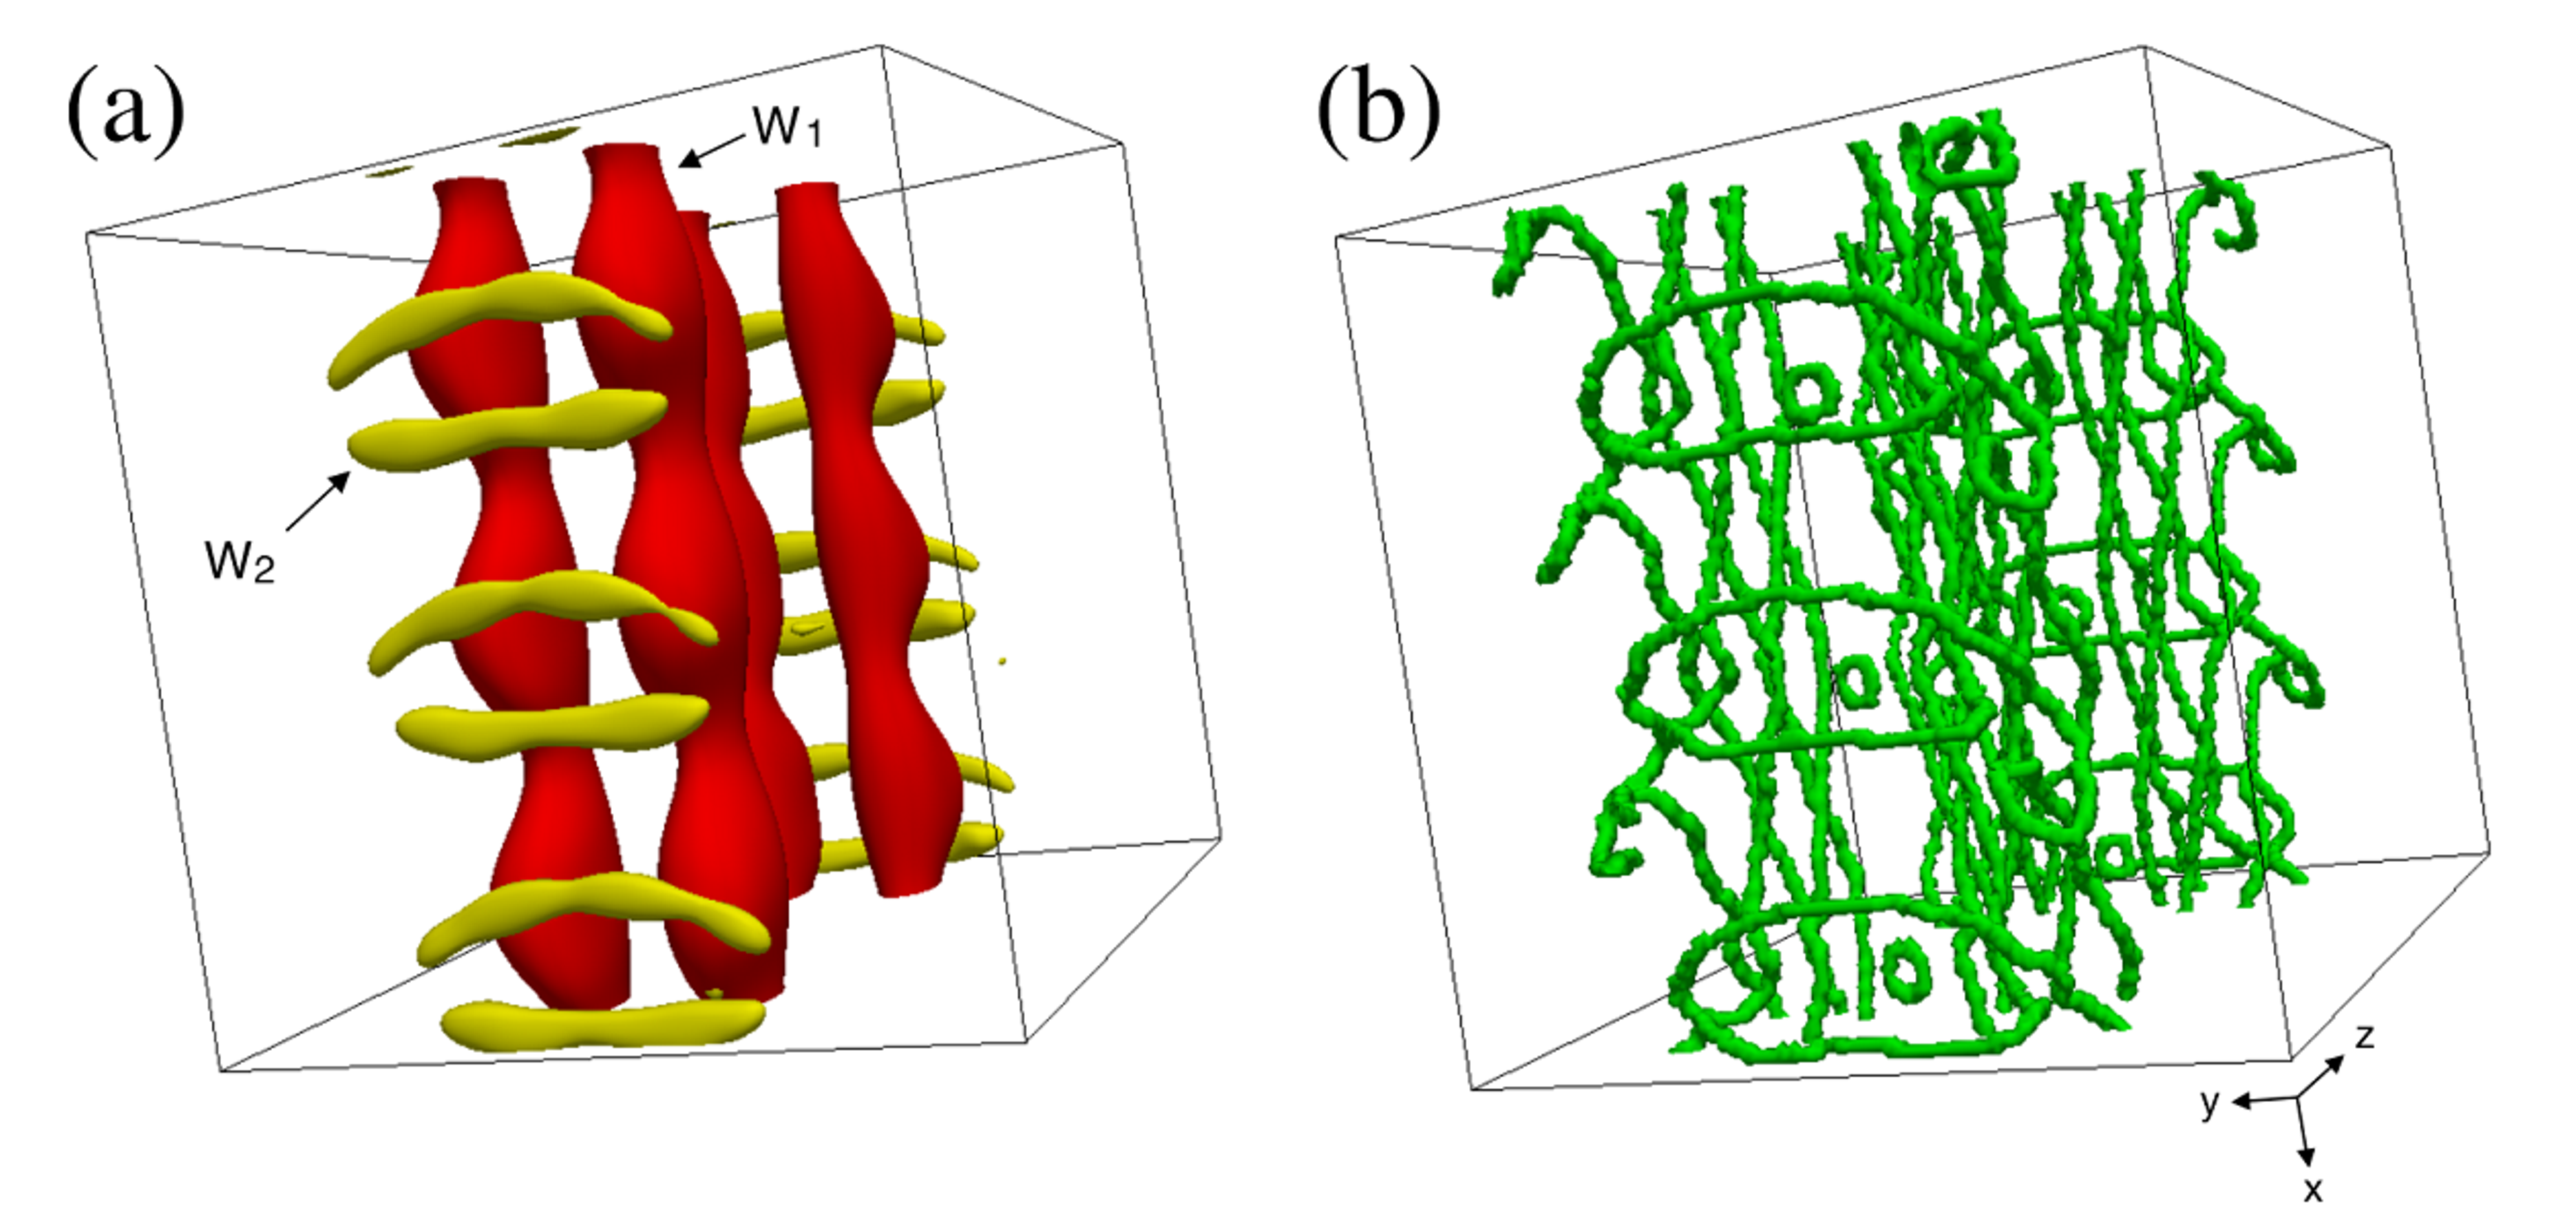
\includegraphics[width=14cm]{cascade.eps}
			\caption{
				(a)は大スケールの渦度$W_1$と小スケールの渦度$W_2$が直交し、渦度分布の階層構造を構成している様子を示す。
                (b)は同じ時刻の量子渦を示す。縦方向の渦芯と、直交するはしご状の横方向の渦芯が配置されている。
                渦度$W_1$の渦伸張により音速付近に達した部分から渦輪が生成され、渦輪と渦度$W_1$の渦芯が
                リコネクションを起こし、直交した高波数の渦度$W_2$が生成される。
                大スケール渦から小スケール渦が生成する
                リチャードソン・カスケードの描像が、量子流体中で起きている。
                詳細は~\ref{s:nucleation}節を参照。
                \\
		        Tsuyoshi Kadokura, and Hiroki Saito,
                \\
		        Orthogonal and antiparallel vortex tubes and energy cascades in quantum turbulence,
                \\
		        Phys. Rev. Fluids {\bf 3}, 104606 (2018).
			}
			\label{FIG:cascade}
			\end{center}
		\end{figure}


		\section{まえがき}
		\ 本研究は超流動体の乱流状態におけるエネルギーカスケードの
        メカニズムを明かにする目的で、渦度を可視化しその渦度分布の階層構造について調査したものである。
		超流動体のマクロな系を記述するGP方程式を用いた平均場近似による
		数値計算をおこないその詳細を分析した。
		分析は以下の二つの手順で進めた。
		はじめに、三次元空間の4ヶ所に大スケールの渦バンドルを配置し初期条件から時間発展させる。
        波数空間をフーリエ変換し、各スペクトルの渦度の位置関係を分析する。
		次に、低波数領域のランダムポテンシャルの外力を与えた
        定常的な一様等方性乱流状態について、はじめの手順で得られた結果と
        どのような共通点があるかを同じ方法で調査を行い考察する。
        調査の結果から、大スケールの渦バンドルを配置した初期条件からの時間発展の様子について、
		フーリエ変換による波数空間のバンドパスフィルタで各スケールの渦度分布を可視化することで、
		大スケールの渦バンドルから直交した小スケールの渦バンドルが生成される
		過程があることがわかった。
		これは渦の分裂に伴い、大スケールの運動エネルギーが小スケールの方向へ向かう
		階層的なエネルギーカスケードと連動していると示唆できる。
		本研究では量子化された渦芯のダイナミクスの可視化による、大スケール渦から小スケール渦生成の詳細な分析も併せて述べる。
		\\
		乱流中ではレイノルズ数の増加により、層流の流れが動的な不安定性を伴いながら
		渦を巻き乱流に発達する~\cite{Reynolds}。
		その運動エネルギーは大スケールの渦から小スケールの渦に向かって
        連鎖、カスケード的に伝達される。
		この様子について古くはレオナルド・ダビンチが排水溝から流れ出る水流で、
		もつれあう大きな渦と小さな渦をスケッチに描かれている。
		その後の記録では、気象学者のリチャードソンが乱流のメカニズムについて
		大きなスケールの渦が小さなスケールの渦へ階層的に分離する
		様子を図.~\ref{FIG:richardson_cascade}~\cite{Richardson}にある文章で残している。
        \begin{figure}[H]
			    \begin{center}
			    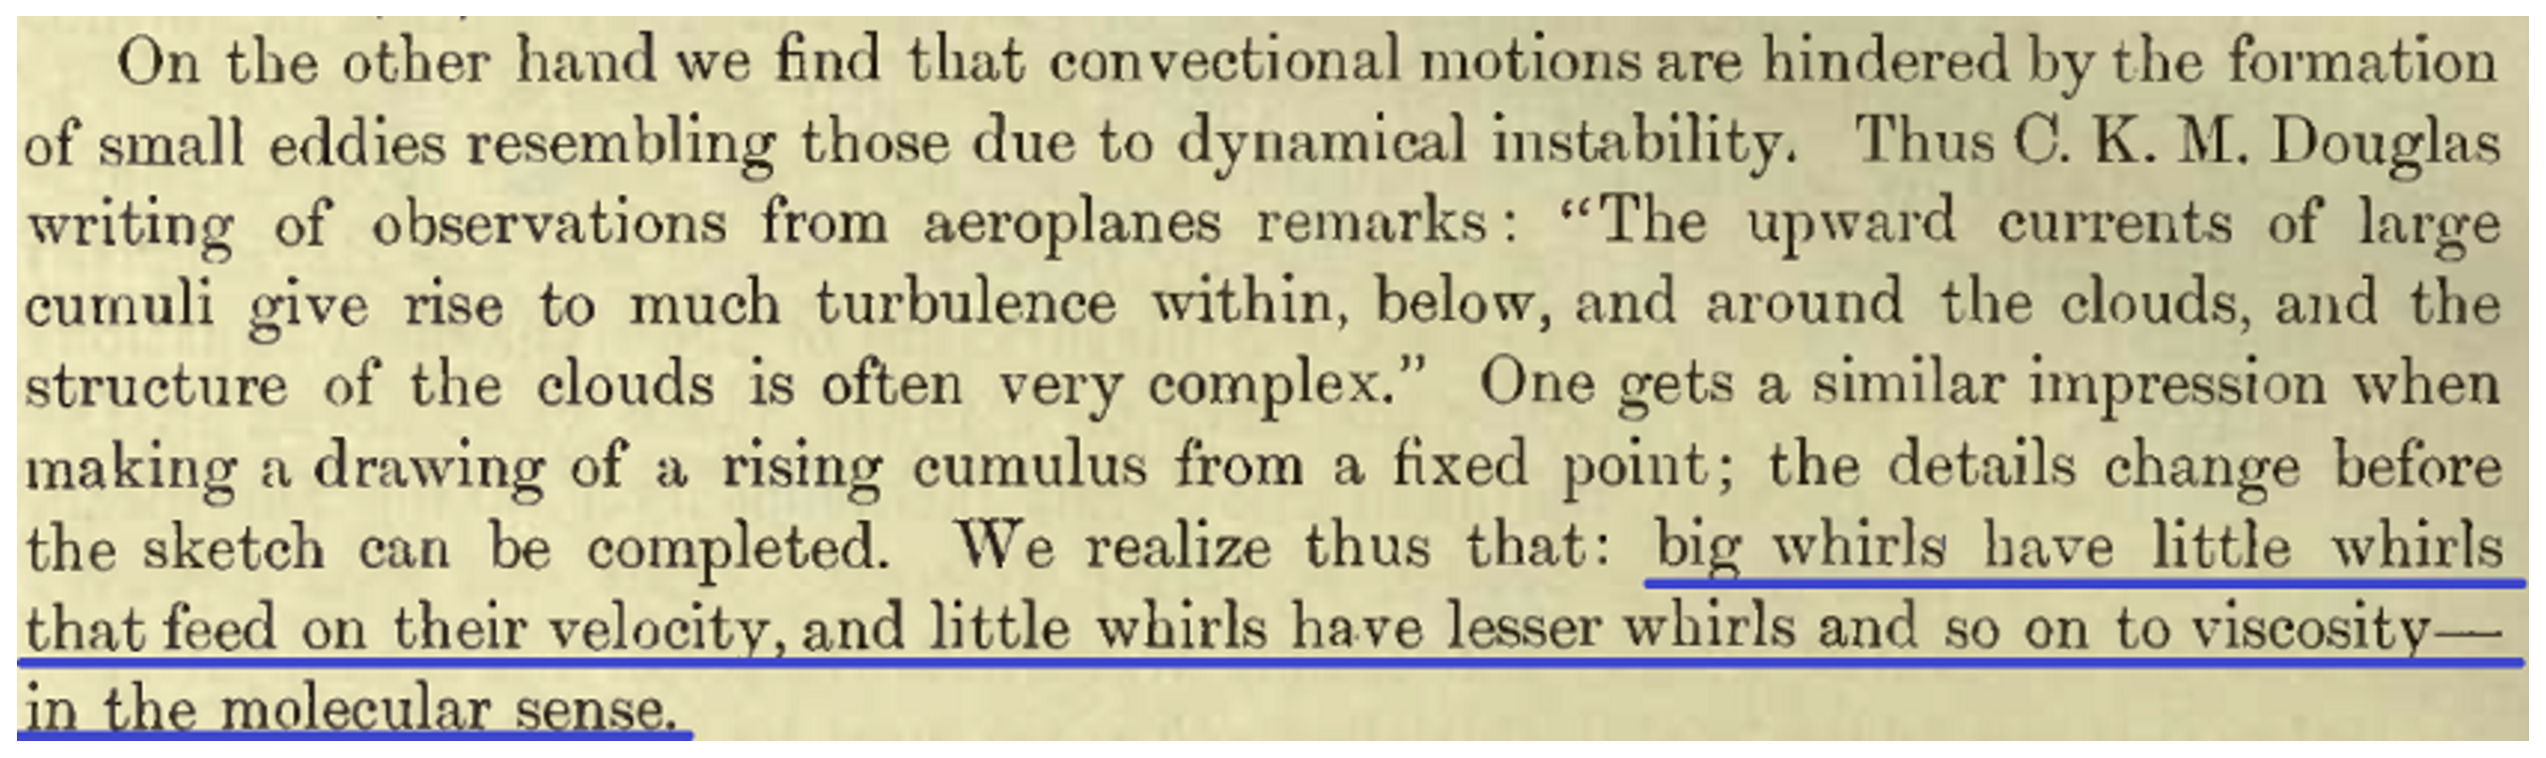
\includegraphics[width=14cm]{richardson_cascade.eps}
			    \caption{
                    リチャードソンの著書からの引用”
                    大きな渦にはその速度に乗った小さな渦が発生し、
                    小さな渦にはより小さな渦が粘性を伴って発生する。
                    ” ~\cite{Richardson}
                }
			    \label{FIG:richardson_cascade}
			    \end{center}
        \end{figure}
		また統計的な立場から、コルモゴロフは乱流中で起きるエネルギーカスケードのスペクトルが$-5/3$のべき乗
		に従うと仮説を立てた。この仮説を実証した研究が理論、実験ともに多くある
		~\cite{Frisch1, Kolmogorov, Batchelor, Tatsumi1, Tatsumi2, Kraichnan, Frisch2, Cyril, Goto1, Goto2}。
		一方、量子流体には量子化される渦度や粘性が無いことなど、古典流体と異なる特徴があるにもかかわらず、
		いくつかの共通した流体現象を示している
        ~\cite{Sasaki1, Reeves1, Kwon0, Sasaki2, Kadokura, Takeuchi0, Bezett}。
		乱流現象についても、超流動ヘリウムや冷却原子ガスによる量子流体において、
		エネルギーカスケードが存在する~\cite{Skrbek, Navon}。
		量子流体の乱流においても非圧縮性の運動エネルギーの
		スペクトルが$-5/3$のべき乗のコルモゴロフ則を示している
		~\cite{Araki, Kobayashi1, Kobayashi2, Kobayashi3}。
		その他にも量子流体の領域で、様々な動力学についてのエネルギースペクトルが研究されている
		~\cite{
		Kerr3, Tsubota2, Kerr1, Nemirovskii, Kolmakov, Barenghi0, Walmsley, Hanninen,
        White, Barenghi2, Fujimoto0, Kobayashi4, Nore, Tabeling, Stalp, Madison, Barenghi1,
        Parker, Walmsley2, Baggaley, Reeves2, Baggaley2, Nemirovskii2, Villois
        }。


		\section{古典乱流における理論的背景}
		古典乱流の先行研究として、後藤らは渦度分布を可視化する側面から、
		数値計算によるエネルギーカスケードの理論的な調査が行われた~\cite{Goto1,Goto2}。
		乱流状態の系の渦度場空間をフーリエ変換し、バンドパスフィルターを用いて、
		各スペクトルの大小の渦度分布を抽出するものである。
		その結果、反平行の大スケールの渦から、直交した配置の小スケール渦が
		生成されるメカニズムがあることを発見した。
		彼らの結論では、エネルギースペクトルの慣性領域では大スケールの渦管伸張により
		小スケールの渦管が生成され、この多段の階層構造がリチャードソンの主張する
		エネルギーカスケードに寄与していると述べている。
		そして大スケールから小スケールに伝搬する
		エネルギーカスケードが$-5/3$べき乗のコルモゴロフ則を示す要因であることを示唆した。
		これらの背景をもとに本研究では、
        量子流体が現象的に古典流体と類似する特徴をもつことを足掛かりに、
		量子乱流においても古典乱流と同様の
		各渦度分布の動力学的過程があると推測し調査を進めた。

		はじめの手順で、量子流体の三次元空間中で、渦度分布の階層構造の現れるかの調査を行った。
		動力学的なメカニズムを明確に知る手段として、一様に分布している超流動の系に、
		反平行の渦バンドルを意図的に配置し、その時間発展を観測した。
		大小の渦度を波数スペクトルのバンドパスフィルタを用いて抽出し、
        渦度の各渦バンドルを渦管として可視化した。
		その結果、反平行の渦管から直交した小スケールの渦管が
		漸化的に同じく反平行で生成されていることがわかった。
		つぎの手順で、$-5/3$べき乗のコルモゴロフ則を満たす発達した一様等方な量子乱流に対して、
		先と同様の波数スペクトルのバンドパスフィルタによる方法で調査した。
		大小の各渦管が向く方向の角度分布を分析した結果、
		古典流体で観測された関係と同様に、量子流体においても
		同じスケールの渦管の対では反平行性を示し、
		大小スケール間の渦管では直交性を示していることを確認した。
		本研究は、~\ref{s:formulation}では理論的な方法とその数値計算について、
		~\ref{s:nucleation}では大スケールの反平行の渦バンドルを配置した初期状態からの時間発展について、
		~\ref{s:distributions}では一様等方的に発達した量子乱流の場合について、
		~\ref{s:conclusions}はこれらの考察とまとめの構成で議論する。


		\section{方法}
		\label{s:formulation}
		本研究では以下に示す三次元空間中の絶対零度による希薄超流動を記述する
		GP方程式の時間発展をモデルに調査を行った。
		\begin{eqnarray}
			\label{eq:GPE}
			\left( i - \gamma \right)
			\hbar \frac{\partial \Psi}{\partial t}
			=
			- \frac{\hbar^2}{2m} \Vec{\nabla}^2 \Psi
			+ U \left(\Vec{r}, t\right) \Psi + \mathrm{g} |\Psi|^2 \Psi,
		\end{eqnarray}
		$\Psi(\Vec{r},t)$は巨視的な波動関数、$m$は粒子の質量、$U(\Vec{r},t)$は外部ポテンシャル、
		$\mathrm{g}$は結合定数を示す。
		式~(\ref{eq:GPE})には、この系の現象論的なエネルギー散逸としてパラメータ$\gamma$を含み
		~\cite{Kobayashi1,Kobayashi2,Kobayashi3}、
		古典流体における熱的な散逸と同様、エネルギーカスケードにより主に高波数領域で散逸する。
        数値計算は擬スペクトル法を用いて算出した。
        具体的には~\ref{s:numeric}(A)で示す。
		$\gamma = 0$の場合、エネルギーカスケードによる高波数領域のエネルギーが蓄積され、
		乱流状態でコルモゴロフ則が成立しなくなる。
		本研究ではエネルギー散逸として$\gamma=0.004$を用いた。
		波動関数は$\tilde{\psi}=n_0^{-1/2.}\Psi$として規格化する。$n_0=|\Psi|^2$はポテンシャル$U$が
		ない条件での原子の粒子密度である。また空間$\xi = \hbar/(m \mathrm{g} n_0)^{1/2}$、
		時間$\tau = \hbar/(\mathrm{g} n_0)$として規格化条件を課す。
		規格化した以下の~(\ref{eq:NGPE})で数値計算を行う。
		\begin{eqnarray}
			\label{eq:NGPE}
			(i-\gamma) \frac{\partial \tilde{\psi}}{\partial \tilde{t}}
			= \left[
				- \frac{1}{2} \tilde{\nabla}^2
				+ \tilde{U}
				+ |\tilde{\psi} |^2
			\right] \tilde{\psi},
		\end{eqnarray}
		ここで $\tilde{\nabla}^2 = \xi^2 \bm{\nabla}^2$、$\tilde{U} = U/({\mathrm g}n_0)$である。
        \\
        エネルギースペクトルは系全体の運動エネルギー
        \begin{eqnarray}
            E_{\rm{kinetic}} = \frac{1}{2} \rm{d} \Vec{r} |\tilde{\Vec{\nabla}}\tilde{\psi}|^2
        \end{eqnarray}
        をフーリエ変換し波数空間で非圧縮成分を抽出して得られる。
        定義の詳細については~\ref{s:pspectrum}(C)で示す。
        \\
		また質量流束は以下の式で与えられる。
		\begin{eqnarray}
			\label{eq:CURRENT}
			{\bm J} = \frac{1}{2 i}
			\left(
				\tilde{\psi}^\dagger \tilde{\nabla} \tilde{\psi} - \tilde{\psi} \tilde{\nabla} \tilde{\psi}^\dagger
			\right) = |\tilde{\psi}|^2 \tilde{\nabla} \phi,
		\end{eqnarray}
		%質量流を可視化するには式***を用いる。
		%可視化後の密度と速度ベクトル場の様子を図***に示す。
		%また、質量流のほかにスピン流という***の特徴を持つ流れがある。
		%可視化するには式***を用い、
		%可視化後の様子を図***に示す。
		%本研究で注目する渦度は質量流の回転から得られる。
		%可視化するには式***の方法をとる。
		%可視化後の様子を図***に示す。
		%質量流の流れにたいし、図***に示す速度のベクトル場の有向線分に沿ったかたちで
		%渦度が存在していることが分かる。
		$\phi$は波動関数$\tilde{\psi}$の位相成分である。
		渦度$\bm{\Omega}$は通常、速度場の回転
		$\bm{\Omega} 
		= \tilde{\nabla} \times (\bm{J} / |\tilde{\psi}|^2) 
		= \tilde{\nabla} \times \tilde{\nabla} \phi$で定義されるが、この場合、量子化された渦芯上の
		座標位置で分母の確率密度ゼロにより、特異点として発散してしまう。
		この特異点を避けるため、ここでは質量流の渦度として、
		\begin{eqnarray}
			\label{eq:VORTICITY}
			{\bm W} \equiv \tilde{\nabla} \times {\bm J},
		\end{eqnarray}
		を定義する。このことで確率密度がゼロの渦芯上の位置でも、発散とはならず連続的な値をとり数値的に取り扱い易くなる。
        定常乱流を与える外力にはランダムポテンシャル$\tilde{U}$を用いる。
        ランダムポテンシャルの詳細については~\ref{s:random}(B)にて示す。


        \subsection{渦度のスペクトル抽出}
		特定の波数スペクトルの渦度を抽出するために、以下の波数空間のバンドパスフィルタを用いる。
		\begin{eqnarray}
			\label{eq:FFT}
			\tilde{{\bm W}}(\bm{k}, t; k_c) = \left\{
				\begin{array}{ll}
					\int {\bm W}({\bm r}, t) e^{-i \bm{k} \cdot {\bm r}}  {\rm d}\bm{r}
					& (k_c/\sqrt{2}< |\bm{k}| <\sqrt{2}k_c)
					\\
					\\
					0 & ({\rm otherwise})
				\end{array}
			\right.,
		\end{eqnarray}
		$k_c$はバンドパスフィルタで抽出する特定の波数を示す。
		抽出された渦度を累積した渦度分布を以下のようにあらわす~\cite{Goto2,Goto3}。
		\begin{eqnarray}
			\label{eq:IFFT}
			{\bm W}(\bm{r}, t; k_c) =
			\frac{1}{V} \sum_{\bm{k}} \tilde{\bm{W}}(\bm{k}, t) e^{i \bm{k} \cdot \bm{r}},
		\end{eqnarray}
		$V=L^3$は系のサイズである。ここで大小の二つのスケール間の渦分布$\bm{W}(\bm{r}, t; k_c)$をくらべるために
		$\bm{W}_1(\bm{r},t:k_c)$と$\bm{W}_2(\bm{r},t:k_c)$をとる。$\bm{W}_2(\bm{r},t:k_c)$の$k_c$は、
        $\bm{W}_1(\bm{r},t:k_c)$よりも高波数とする。


		\subsection{渦度のスペクトル間の角度分布の分析}
		バンドパスフィルターにより抽出した各スペクトルの渦度から、
        $\bm{W}_1(\bm{r},t:k_c)$と$\bm{W}_2(\bm{r}+\Delta\bm{r},t:k_c)$の間の直交性について、
        角度$\theta_{12}$を得るため、
        余弦定理を用いて角度を算出し任意の領域の出現頻度から角度分布の、
		\begin{eqnarray}
			\label{eq:ORTH}
			\cos \theta_{12}
			\equiv \frac{{\bm W}_1({\bm r},t:k_c) \cdot {\bm W}_2({\bm r} + \Delta {\bm r},t:k_c) }
			{
				|{\bm W}_1({\bm r},t:k_c)| |{\bm W}_2({\bm r} + \Delta {\bm r},t:k_c)|
			}.
		\end{eqnarray}
        を定義する。
		同じスペクトルの渦度の反平行性について、$\bm{W}_1(\bm{r},t:k_c)$と
        $\bm{W}_1(\bm{r}+\Delta\bm{r},t:k_c)$の間の角度$\theta_{12}$を得るため、
		\begin{eqnarray}
			\label{eq:ANTI}
			\cos \theta_{11}
			\equiv \frac{{\bm W}_1({\bm r},t:k_c) \cdot {\bm W}_1({\bm r} + \Delta {\bm r},t:k_c) }
			{
				|{\bm W}_1({\bm r},t:k_c)| |{\bm W}_1({\bm r} + \Delta {\bm r},t:k_c)|
			}.
		\end{eqnarray}
		を定義する。また、$\cos \theta_{12}$と$\cos \theta_{11}$は、
		幅$|\Delta{\bm r}|$に制限した$\bm r$と$\Delta{\bm r}$の渦度ベクトル間で算出する。
		以上の条件を全空間で分析する。$P_{12}(\cos \theta_{12})$と$P_{11}(\cos \theta_{11})$は、
		$\bm r$の座標位置での
		渦度分布間$\Delta{\bm r}$の範囲で得られる角度の頻度分布をあらわす。
		座標位置${\bm r}$と$\bm{r}+\Delta \bm{r}$の間の渦度分布${\bm W}_1$の対が反平行性の
		傾向がある場合、$\cos \theta_{11}=-1$にピークを示し、
		また渦度分布の大スケールの${\bm W}_1(\bm{r})$から生成された
		小スケール${\bm W}_2(\bm{r}+\Delta \bm{r})$の間では
		直交性の傾向がある場合、
		$\cos \theta_{12}=0$にピークを示すことになる。
		$\bm{W}_1$と$\bm{W}_2$のこれらの傾向については次章で述べる。



		以上の方法をもとに、一辺が$L$の立方体$L^3=128^3$の周期的境界条件を課した三次元空間で、
        分解能が$\Delta x = \Delta y = \Delta z = 1$の系による
		擬スペクトル法を用いた数値計算を行い~(\ref{eq:NGPE})の解をもとめる。
        数値計算の詳細については~\ref{s:numeric}(A)にて示す。
		%渦度スペクトル間の反平行性、直交性を確認すべく式**を用いて
		%渦バンドル配置の系に対して、確認を行った。
		%先ず初期値の渦バンドル配置は、図**に可視化したように、反平行を示す。
		%これを式**を用いて期待値である**を確認した。
		%次にこの系は時間発展とともに高波数側のスペクトルの直交した渦バンドルがあらわれることが
		%分かった。この直交性について、式**を用いて期待値である**を確認した。
		%方法は以下のとおりである。


		\section{結果と考察}
    		\subsection{反平行渦バンドルの配置による渦度分布のカスケード過程}
            \label{s:nucleation}
    		\begin{figure}[H]
    			\centering
    			%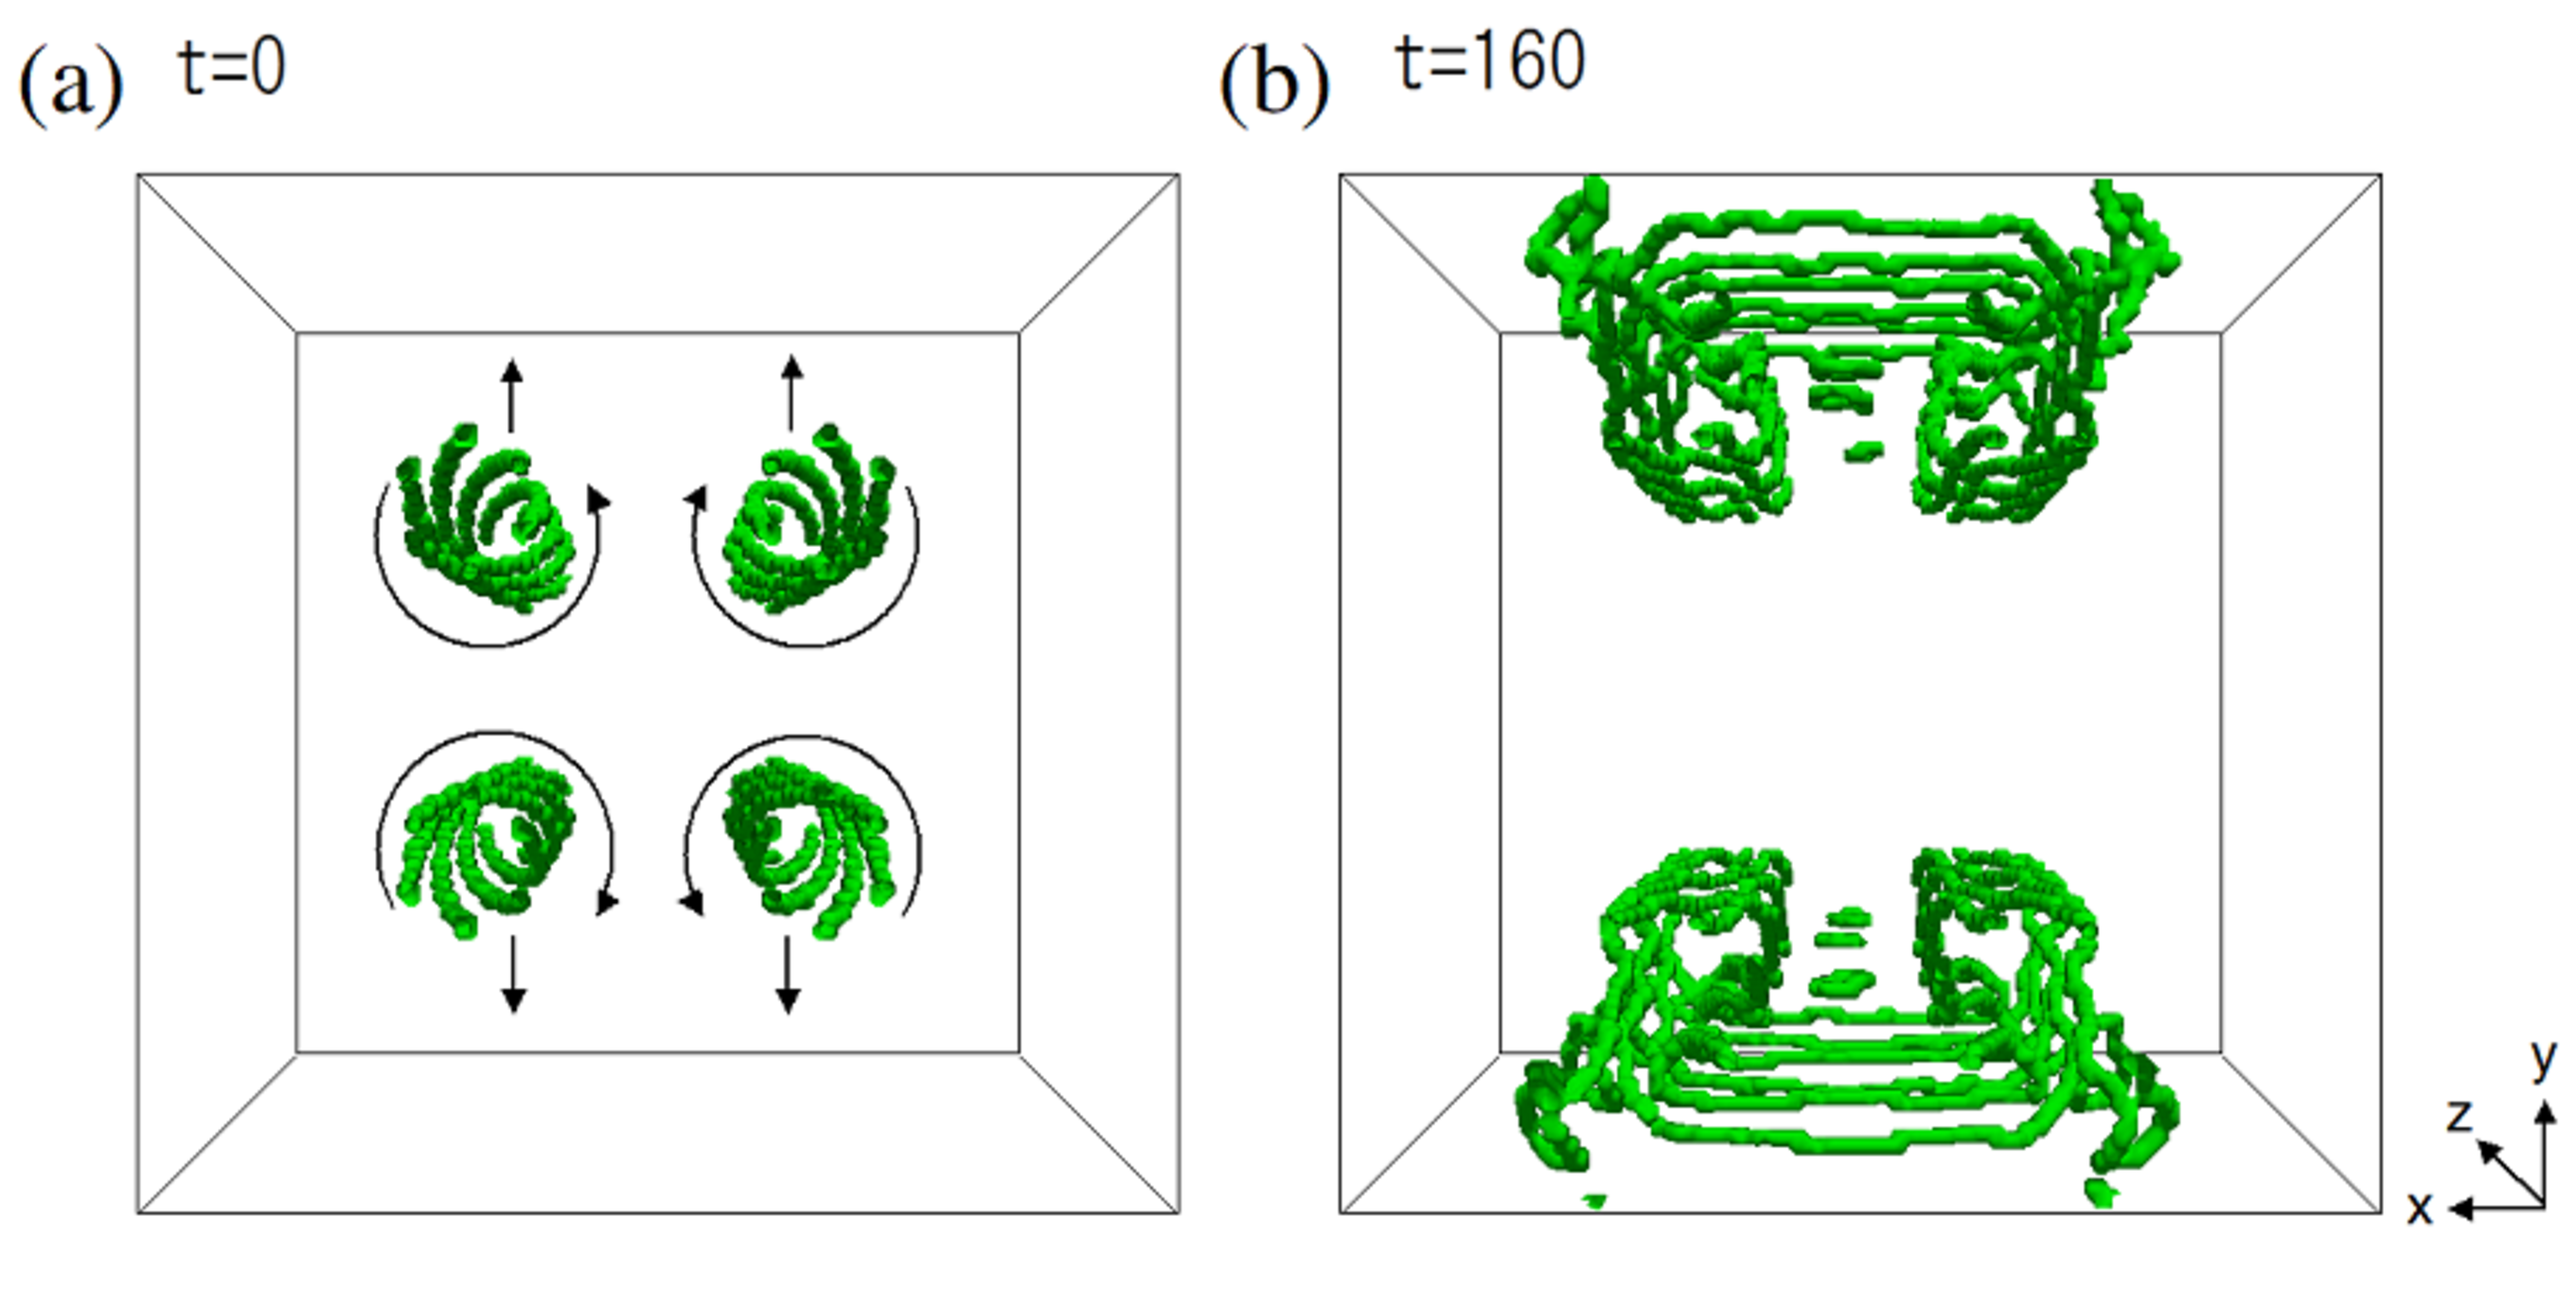
\includegraphics[width=17cm]{fig11.eps}
    			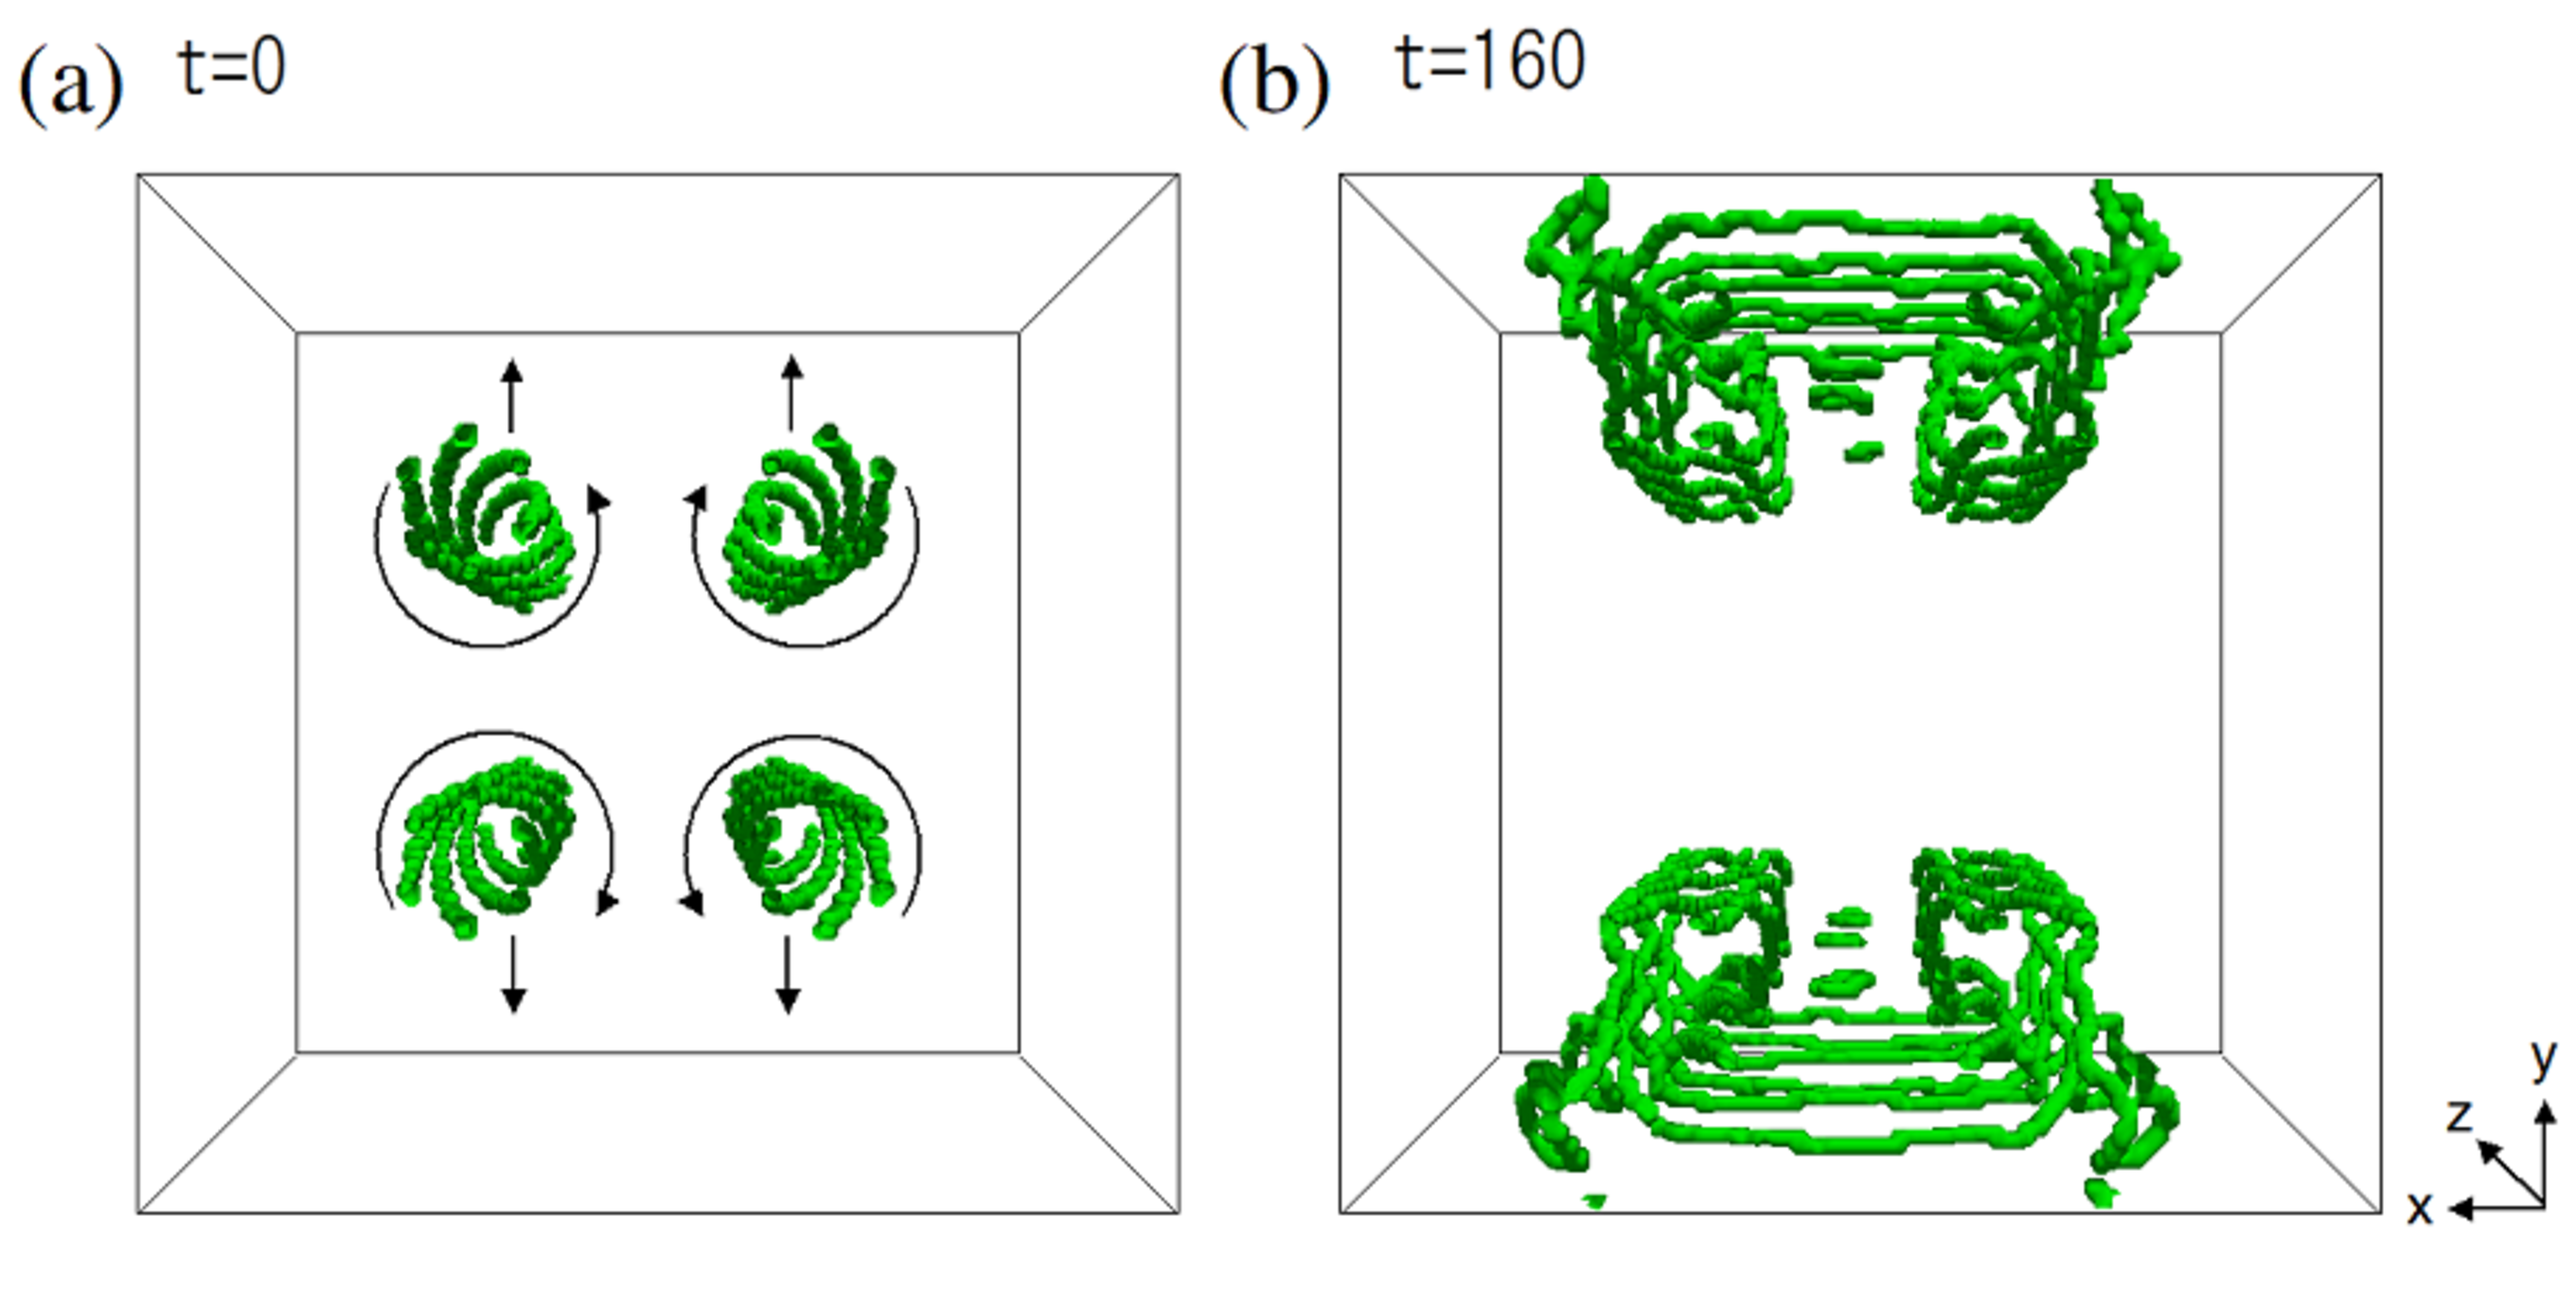
\includegraphics[width=15cm]{fig11.eps}
    			\caption{
    				4つの渦バンドルによる初期状態からの
    				量子化された渦芯のダイナミクスを示す。
    				渦芯は波動関数の位相が$2\pi$に回転した箇所を抽出し可視化してある。
    				\
    				(a) 一様な系に、式~(\ref{eq:SETUPEQ1})で定義した半径16の
    				6本で構成される渦バンドルを
    				中心位置$(x,y)=(64,64),(108,64),(64,108),(108,108)$の4か所に配置。
    				\
    				回転の矢印は渦バンドルの回転方向を示し、$\pm y$の矢印は、
    				渦バンドル自身が移動する方向を示す。
    				(b)は時刻$t=160$のスナップショット。
    				二つの渦バンドルのペアが$pm y$方向に移動していくなか、渦輪とはしご構造の形成が見られる。
				}
				\label{FIG:SETUP}
			\end{figure}
			はじめに、大スケールの渦バンドルがどのように小スケールの渦を生成するかを
			観測するため、乱流を用いず予め大スケールの渦バンドルを配置した初期状態を用意し
            そのダイナミクスを調査した。
			図.~\ref{FIG:SETUP} (a)のように、一様系の三次元空間に、4つの大スケールの渦バンドルを配置する
			~\cite{Yasuda}。
			それぞれの渦バンドルは、以下の数式に示す6本の渦芯で構成される。
			\begin{eqnarray}
				\label{eq:SETUPEQ1}
				\tilde{\psi}({\bm r}) =
				\tilde{\psi}_0({\bm r}) \prod_{n=0}^5
					\frac{x - x_n \pm i(y - y_n)}
					{|x - x_n \pm i(y - y_n)|},
			\end{eqnarray}
			\begin{eqnarray}
				\label{eq:SETUPEQ2}
				\left(
					\begin{array}{l}
						x_n
						\\
						\\
						y_n
					\end{array}
				\right) =
				\left(
					\begin{array}{l}
						r_b \cos \left( \frac{n \pi}{3} \pm \frac{\pi z}{L} \right)
						\\
						\\
						r_b \sin \left( \frac{n \pi}{3} \pm \frac{\pi z}{L} \right)
					\end{array}
				\right), \ (n=0, 1, \cdots, 5),
			\end{eqnarray}
			数式~(\ref{eq:SETUPEQ1})の$\tilde{\psi}_0$は波動関数を示し、
			$r_b$はバンドルの半径サイズ、渦芯の回転方向は$\pm$符号で定義する。
			この系では数式~(\ref{eq:NGPE})において、ポテンシャル$\tilde{U}=0$としてある。
        

            %量子渦のバンドルの初期状態は具体的に以下の手順で計算する。
            %\\
            %1.$X=0 \sim 127, Y=0 \sim 127, Z=0 \sim 127$の三次元空間の、
            %\\  $XY$平面の$4$ヶ所に$6$本ずつ量子渦を配置する。
            %\\
            %2.$Z$軸方向にスパイラル状の構造となるようにする。
            %\\  $4$ヶ所のバンドルが反平行のスパイラルの向きにする。
            %\\
            %3.はじめに一様な波動関数$\psi[X][Y][Z]=1.0 + i0.0$を$128^3$全体に書き込む。
            %\\
            %4.$XY$平面に、量子渦のバンドルを書き込む$4$ヶ所の、
            %\\  $(X_n,Y_n)=(64,64),(108,64),(64,108),(108,108)$の位置にそれぞれ、
            %\\  半径$R=8$の太さのバンドルとして、$6$本の量子渦を$(X_n,Y_n)$を中心に
            %\\  $\theta_n = (\theta_1, \theta_2, \theta_3, \theta_4, \theta_5, \theta_6) 
            %= 2 \pi (0/6, 1/6, 2/6, 3/6, 4/6, 5/6)$の角度に配置するため、
            %\\  波動関数に$\psi=\psi \exp \left[ i \tan^{-1} (y/x) \right]$の位相成分を付加する。
            %\\
            %5.$y$は、$y \equiv (Y-Y_n)+R \sin(\pi /128)Z + \theta_n$で定義される。
            %\\  $Y$は$0 \sim 127$、$Z$は$0 \sim 127$の範囲。
            %\\
            %6.$x$は、$x \equiv (X-X_n)+R \cos(\pi /128)Z + \theta_n$で定義される。
            %\\  $X$は$0 \sim 127$、$Z$は$0 \sim 127$の範囲。
			%図.~\ref{FIG:qv_put}は、上記の手順で渦芯を配置した例を示す。
			%\begin{figure}[H]
			%	\centering
			%	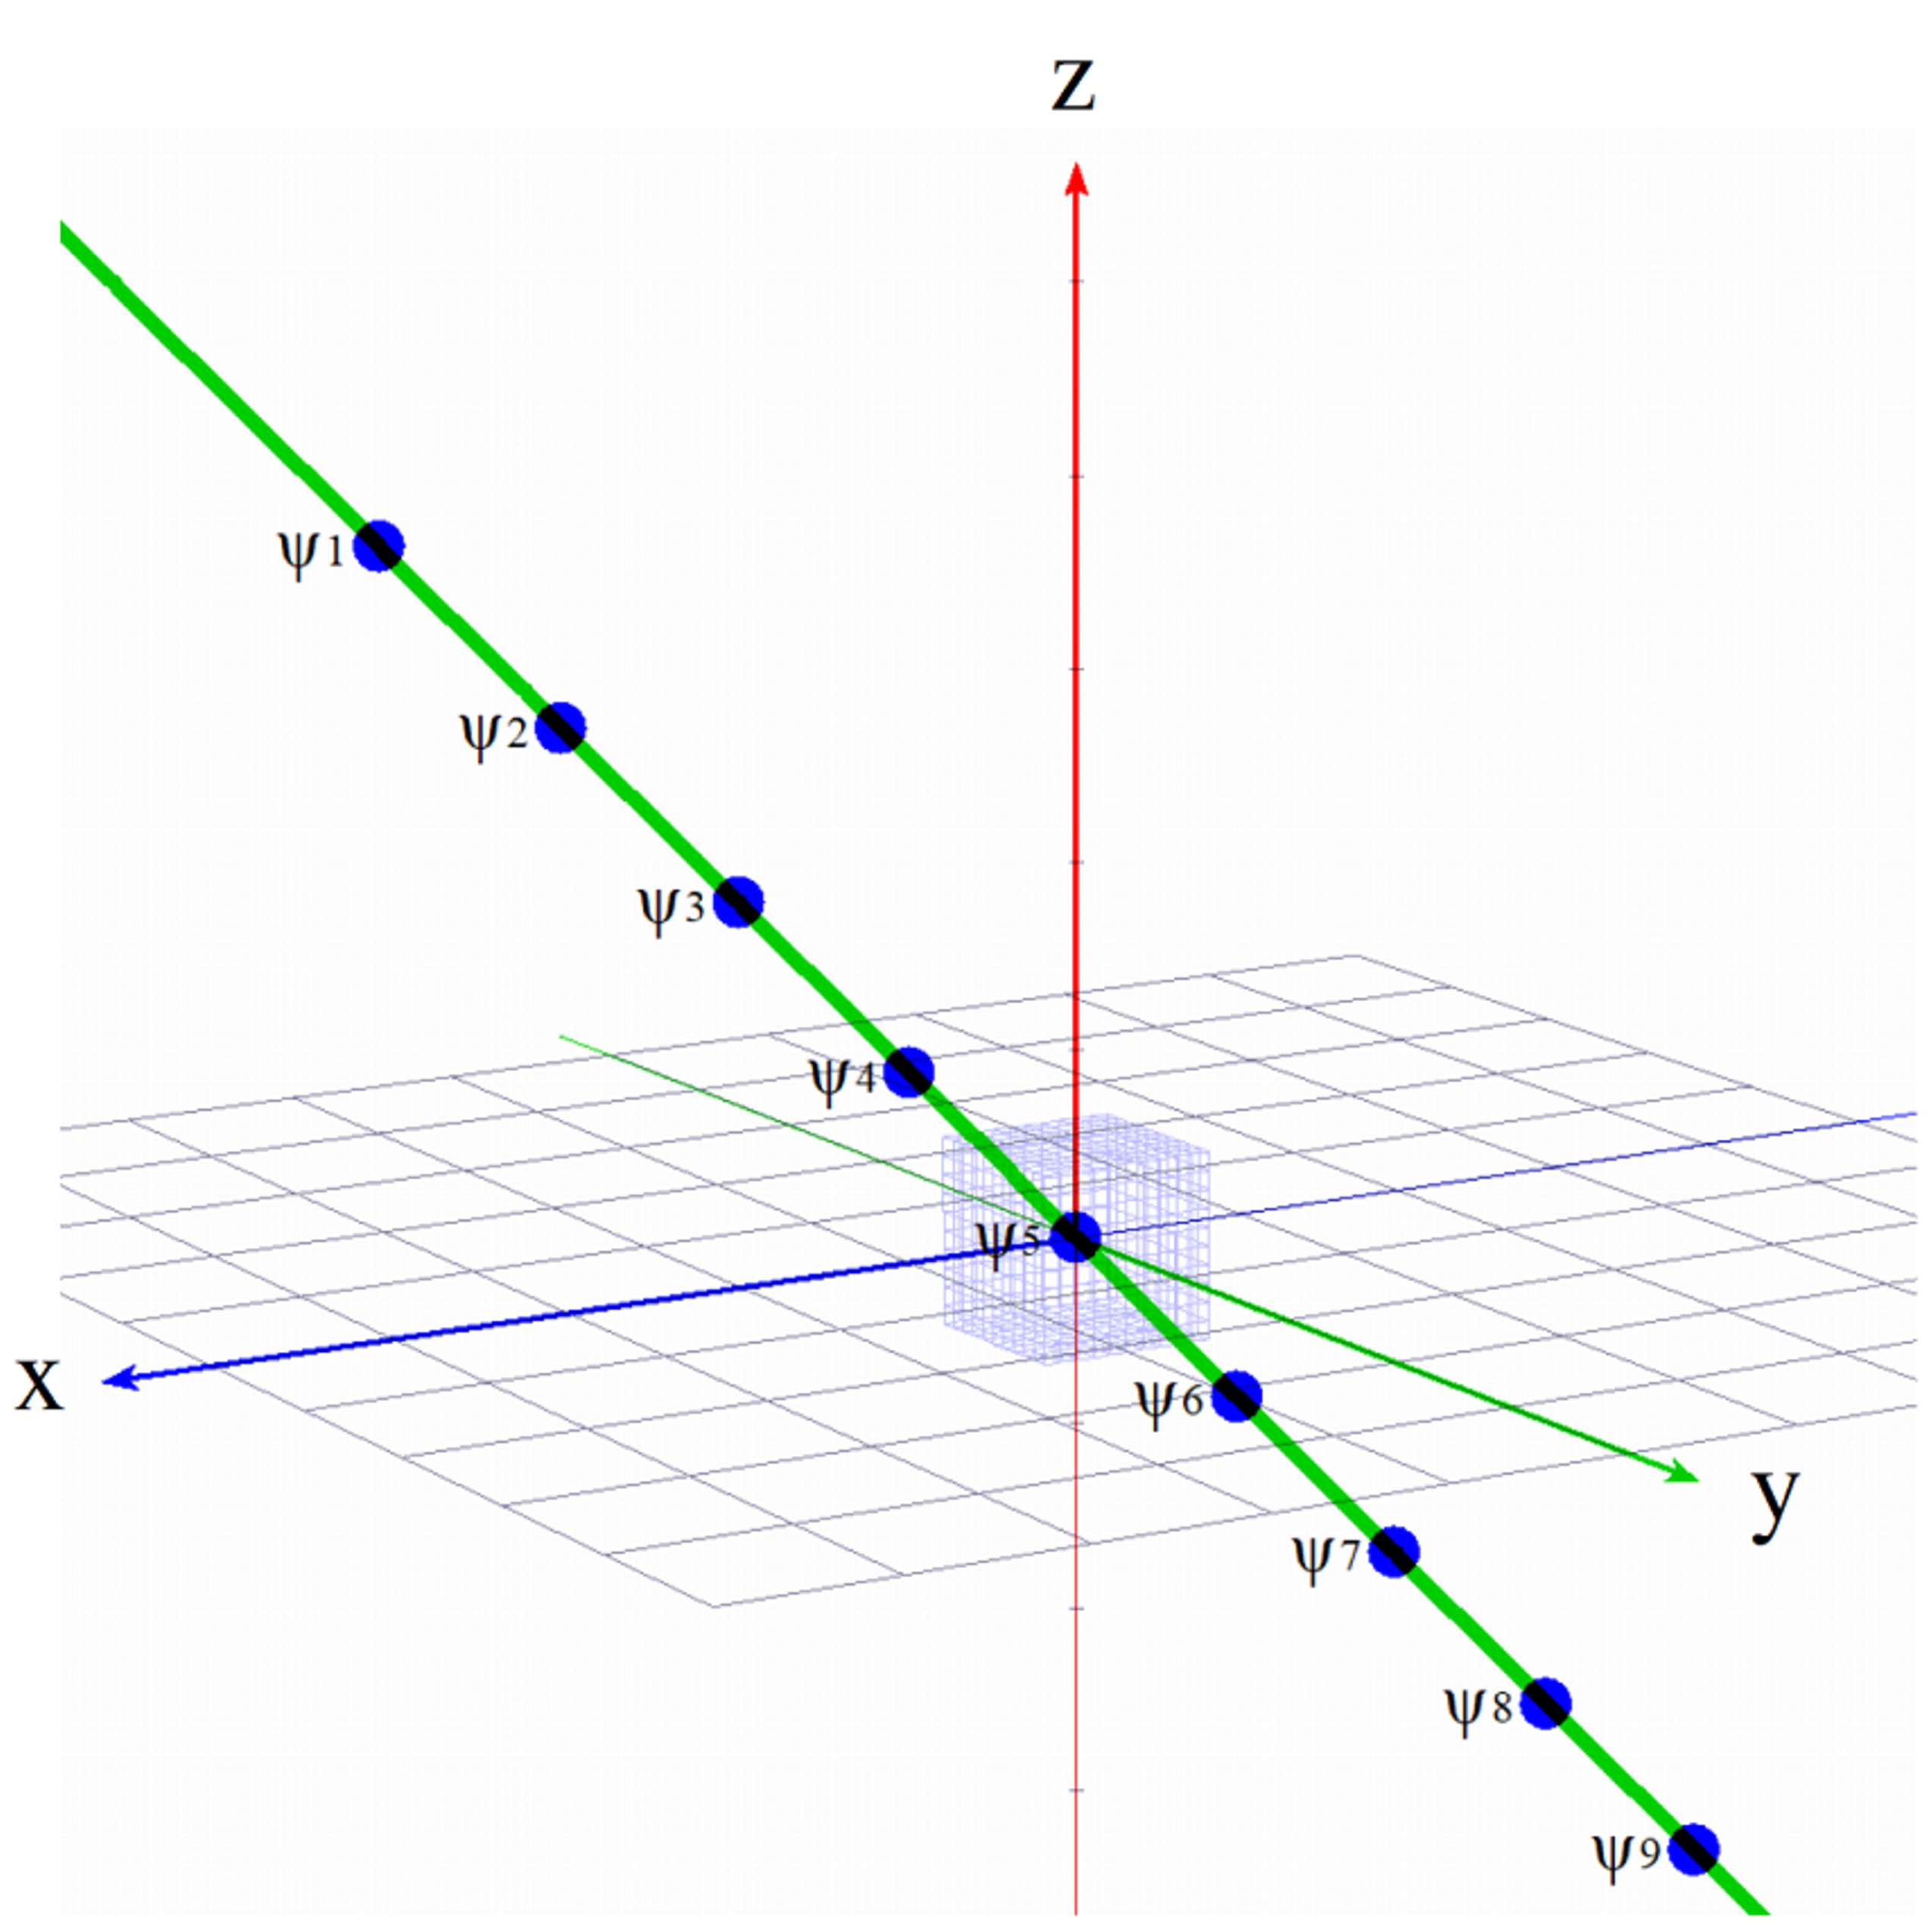
\includegraphics[width=10cm]{qv_put.eps}
			%	\caption{
			%		渦芯を配置する座標の波動関数$\Psi_1$から$\Psi_9$に位相$ \sim e^{i2\pi}$を付加する。
			%	}
			%	\label{FIG:qv_put}
			%\end{figure}

			図.~\ref{FIG:SETUP}は、波動関数の値から
            位相差のデータを算出し渦芯の情報を抽出したものである。
            \\
            \\
            \\
             具体的には以下の手順で計算する。
            \\
            1.数値計算上の空間$XYZ=128^3$に入る波動関数のデータは複素数で表現される。
            \\  $X$、$Y$、$Z$は波動関数の値が入る空間の座標の整数値$0 \sim 127$で、
            \\  全空間にわたって値を読み取る。
            \\
            2.座標位置を中心とした回転面上の周囲$8$ヶ所の位相差を以下の様に合計する。
            \\
                図.~\ref{FIG:qv_det}の例)
            \\
                $\psi_1(X-1,Y-1,Z+1)$、$\psi_2(X-1,Y,Z+1)$、$\psi_3(X-1,Y+1,Z+1)$、
            \\
                $\psi_8(X, Y-1,Z  )$、    中心、   $\psi_4(X, Y+1,Z )$、
            \\
                $\psi_7(X+1,Y-1,Z-1)$、$\psi_6(X+1,Y,Z-1)$、$\psi_5(X+1,Y+1,Z-1)$
            \begin{eqnarray}
            \theta_{\rm{sum}} & = & \arg(\psi_1/\psi_2)
            +\arg(\psi_2/\psi_3)
            +\arg(\psi_3/\psi_4)
            +\arg(\psi_4/\psi_5) \nonumber
            \\
            & &
            +\arg(\psi_5/\psi_6)
            +\arg(\psi_6/\psi_7)
            +\arg(\psi_7/\psi_8)
            +\arg(\psi_8/\psi_1),
            \end{eqnarray}
            \\
              合計した$\theta_{\rm{sum}}$が$2 \pi$の条件を満たした中心の座標を$1$、
            \\
              それ以外を$0$として渦芯の有無を判定し抽出する。
            \\
            3.さらにその座標を中心として、回転面の向きを以下の$9$方向から同様の判定で調べる。
            \\
              $z$軸に直交する$x-y$面、$x$軸に直交する$y-z$面、$y$軸に直交する$x-z$面、
            \\
              $z$方向に$45$度傾いた$x-y$面、$z$方向に$135$度傾いた$x-y$面、
            \\
              $x$方向に$45$度傾いた$y-z$面、$x$方向に$135$度傾いた$y-z$面、
            \\
              $y$方向に$45$度傾いた$x-z$面、$y$方向に$135$度傾いた$x-z$面、
            \\
			  図.~\ref{FIG:qv_det}では上記の手順の、$x$方向に$135$度傾いた$y-z$面の場合である。
			\begin{figure}[H]
				\centering
				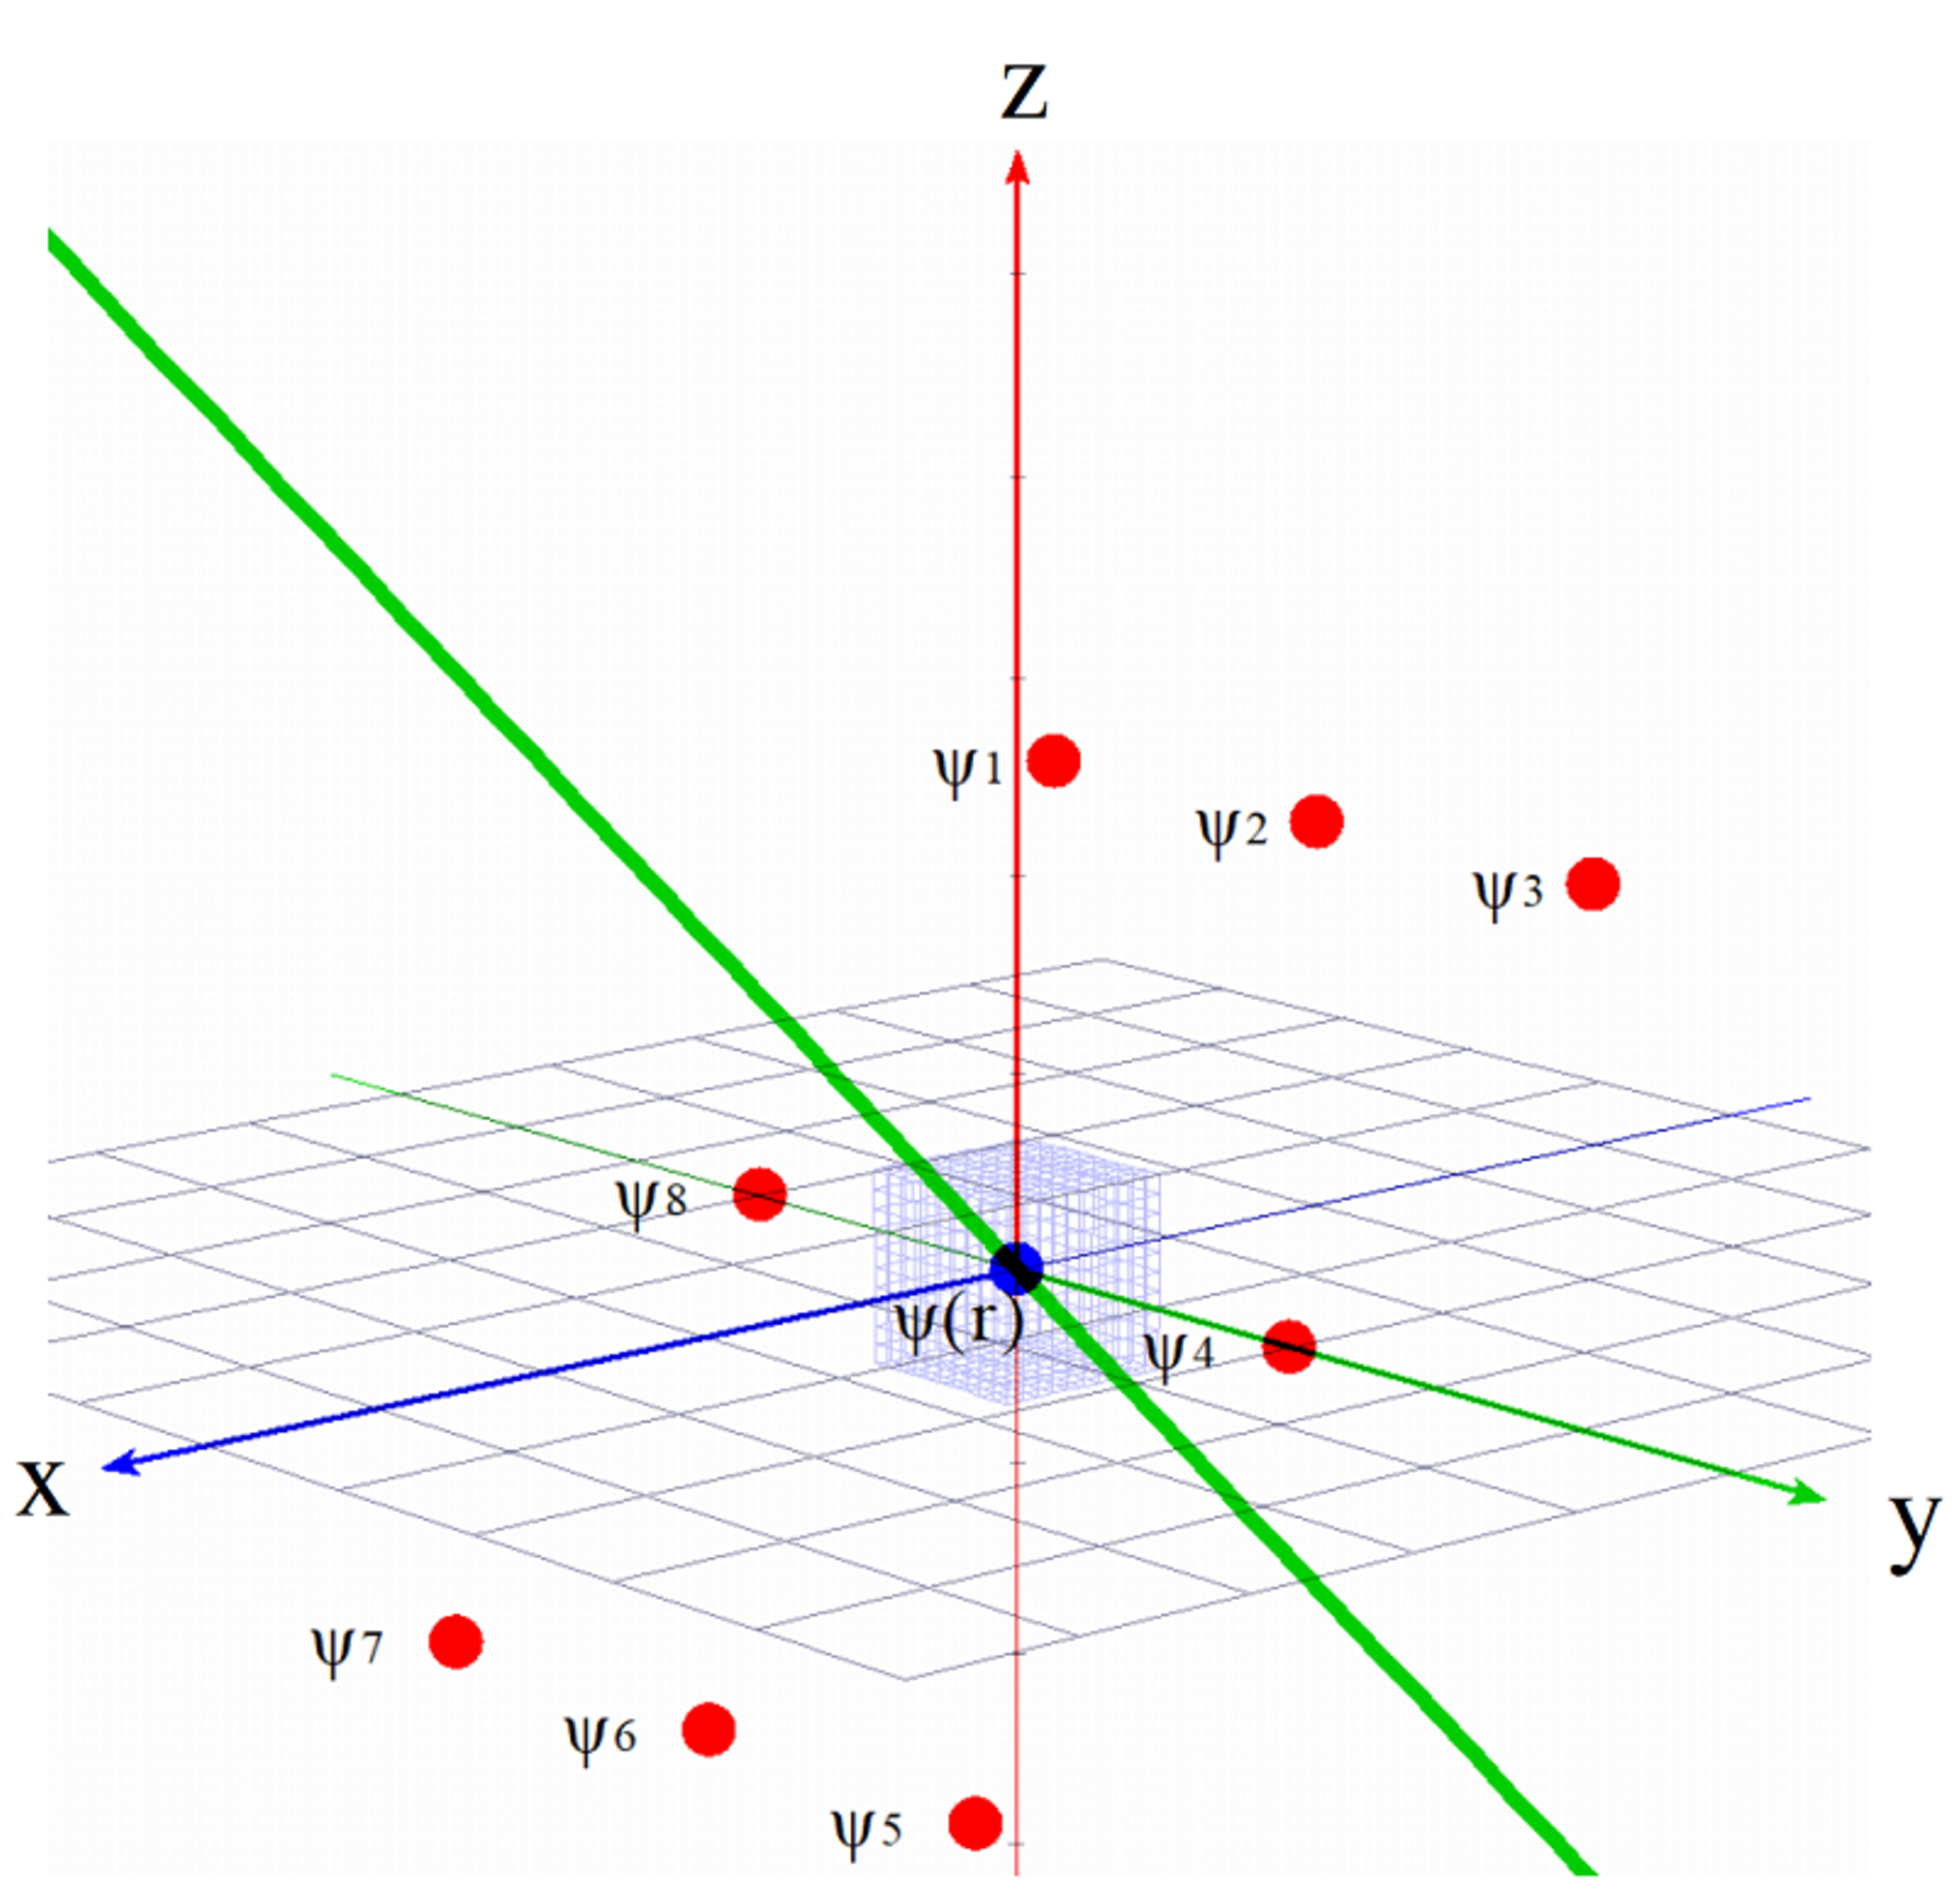
\includegraphics[width=12cm]{qv_det.eps}
				\caption{
					全空間を走査し、座標位置を中心とする回転面の周囲$8$ヶ所の波動関数のデータから位相差
                    を合計する。
                    合計が$2 \pi$の場合、渦芯ありと判定する。
                    回転面の向きは全方位$9$方向から渦芯を抽出する。
				}
				\label{FIG:qv_det}
			\end{figure}


			図.~\ref{FIG:SETUP}(a)は初期状態から、二つの渦バンドルのペアは$\pm y$方向に対向して進む。
			ねじれた構造は、渦バンドルの渦芯が遠心力によってすぐに広がってしまわない目的である。
			時間発展が進むと、バンドルの間から小さな渦輪が生成、伸張する。
			さらに生成される後方の新たな渦輪により、はじめの渦輪は押し出され
            渦バンドルの渦芯とリコネクションを起こす。
			図.~\ref{FIG:SETUP}(b)のように渦輪は変形した後、バンドルに対して直交したはしご状の構造をとる。
            また、三次元空間の大きさ$128^3$に対して空間の分解能を$0.5$としているため、
            図.~\ref{FIG:SETUP}の渦芯は$2$の太さで可視化される。

            初期状態の図.~\ref{FIG:vbndl}(a)~(d)は、図.~\ref{FIG:SETUP}(a)と同じ結果の
            $z=64$の断面について示す。
            $6$本で構成した渦芯を
			図.~\ref{FIG:vbndl}(b)は$z=64$での密度分布の断面で、$6$本の渦芯で構成した
            大スケールの渦バンドルが4ヶ所に配置しているのがわかる。
			図.~\ref{FIG:vbndl}(c)はその速度場を示し、
            それぞれの渦芯をすべて同じ向きの回転方向にすることで、大きなスケールの渦として構成できる。
            図.~\ref{FIG:vbndl}(d)は波動関数から位相を算出し、渦芯の存在の有無と回転方向が確認できる。
			この渦バンドルの大スケールの渦を時間発展させて、
            小スケールの渦へカスケード分裂する過程を算出する。
			\begin{figure}[H]
				\centering
				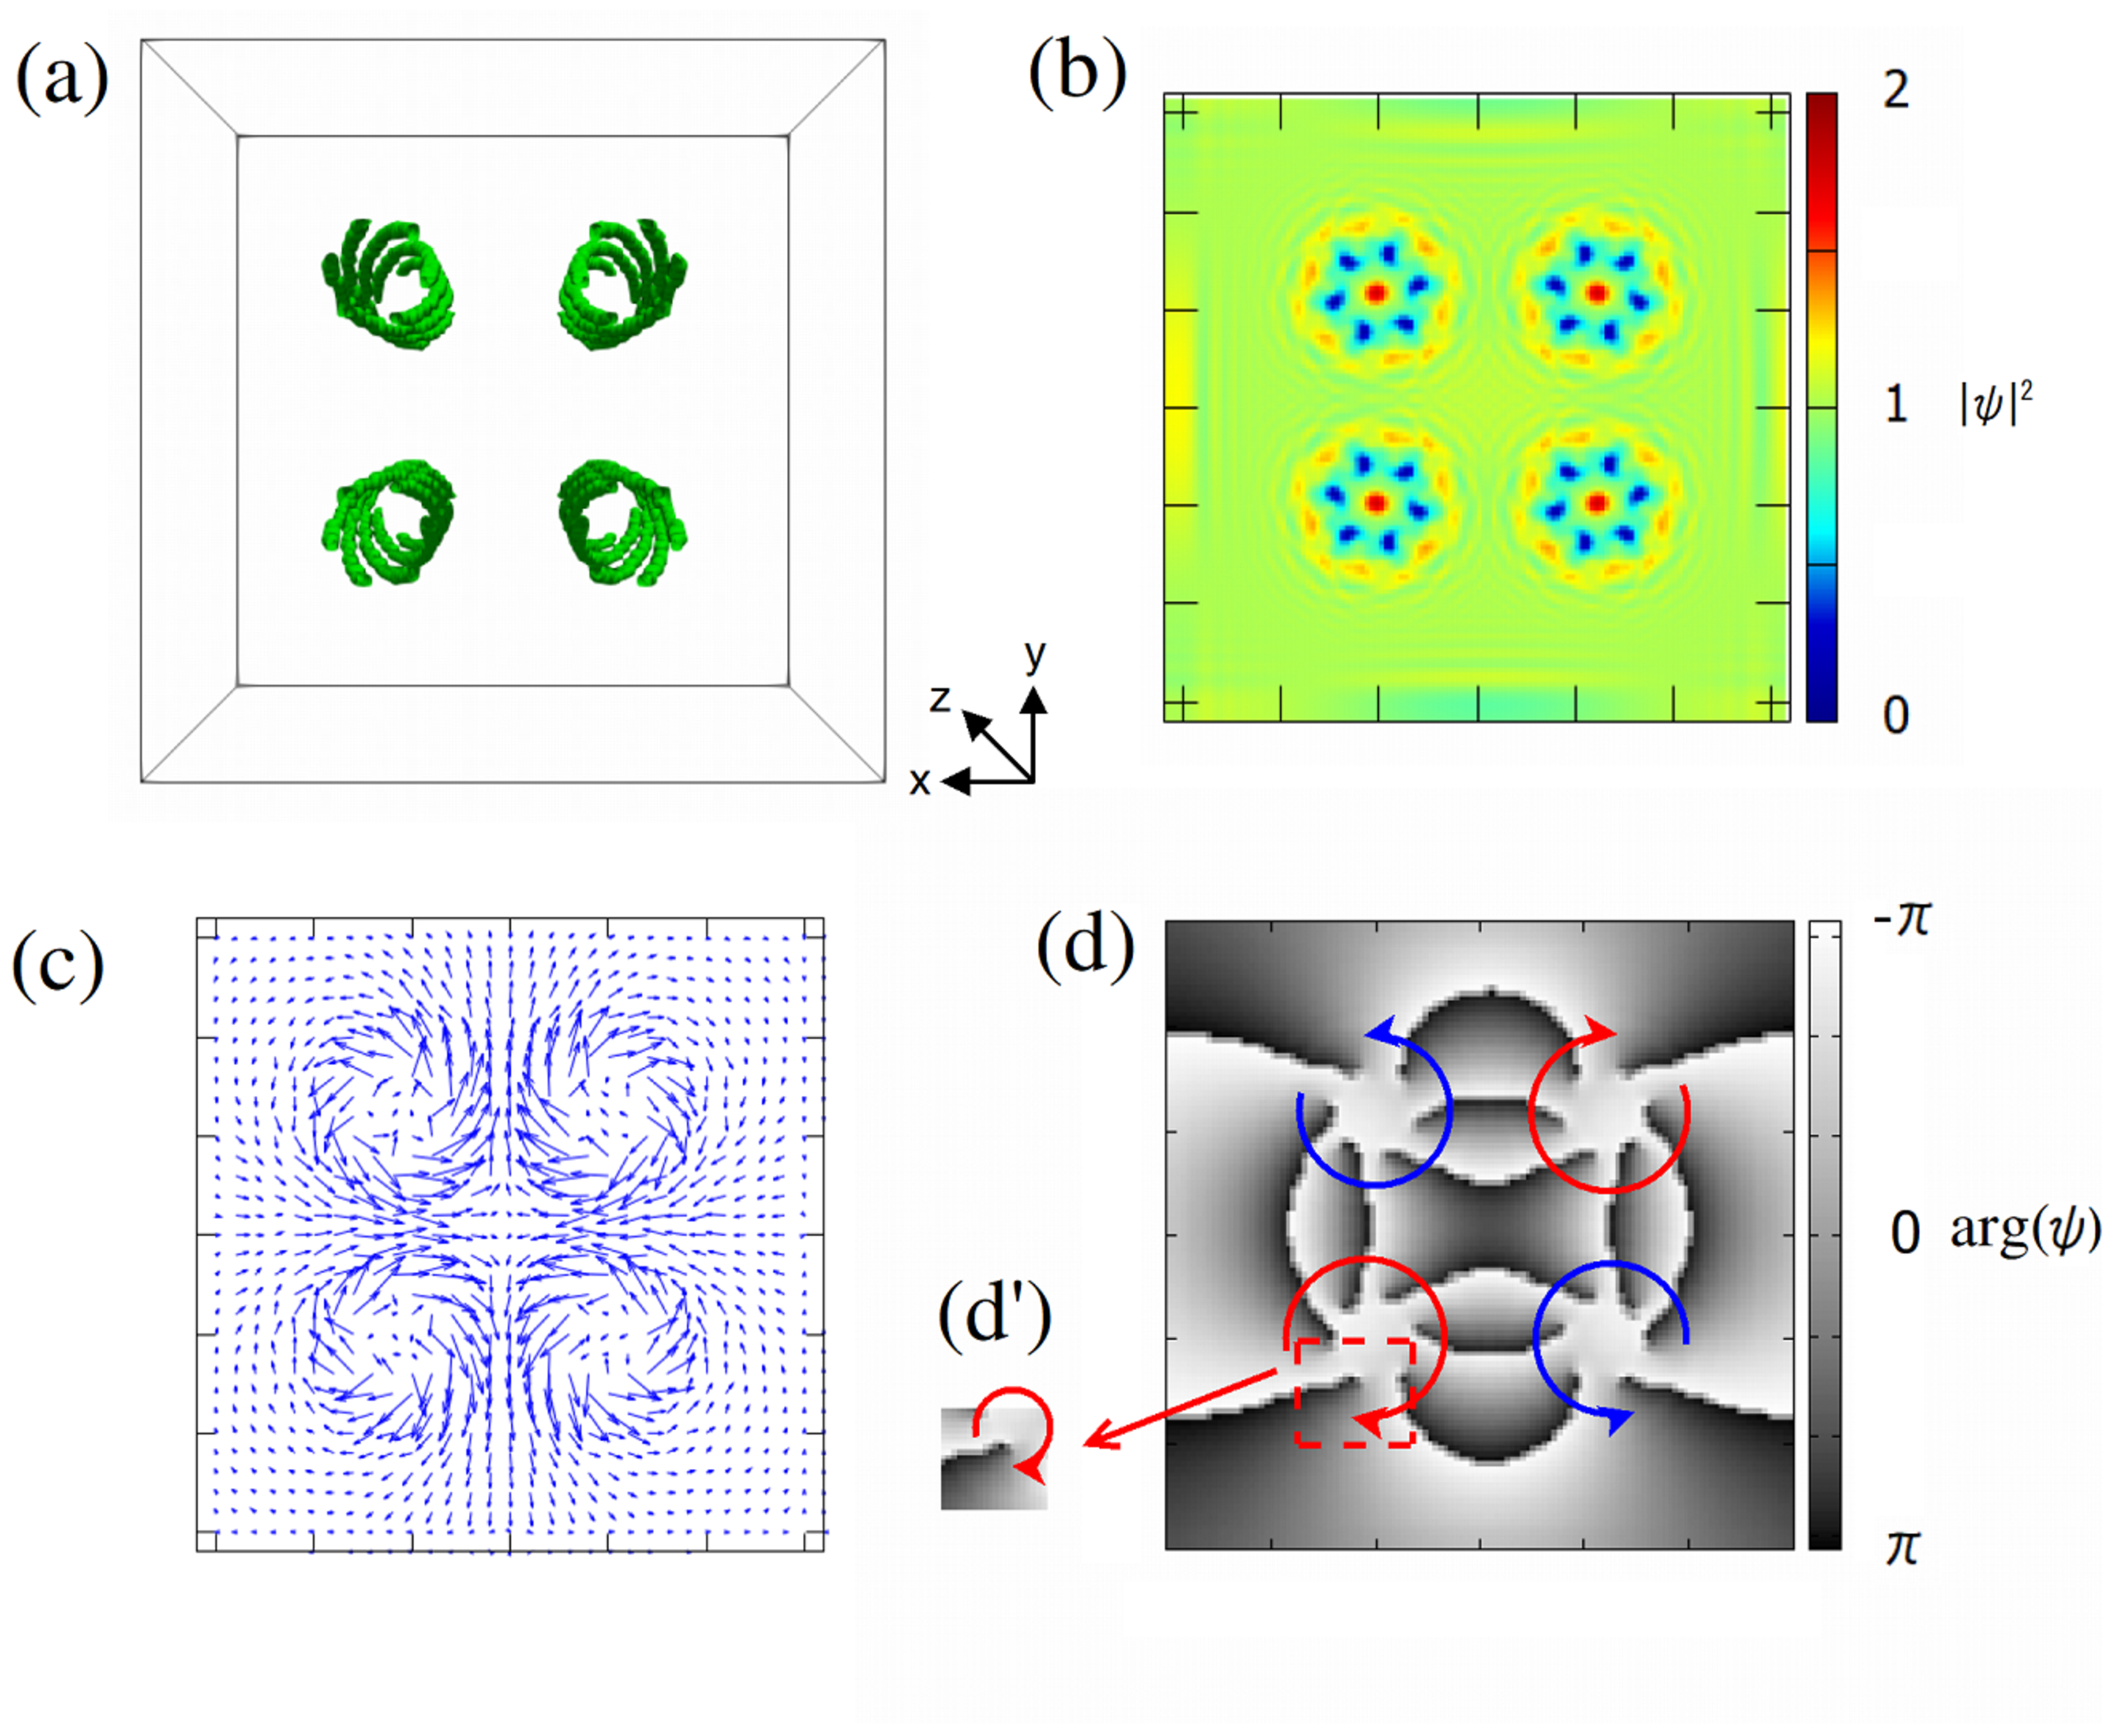
\includegraphics[width=16cm]{vbundle.eps}
				\caption{
					(a)は、渦芯$6$本の渦バンドル構造を4ヶ所に対称に配置した初期状態。
					(b)は$z=64$での密度分布の断面。
					(c)は、(b)の速度場のベクトルを示す。
                    速度ベクトルの向きから、大スケール(低波数)の渦が互いに反平行に配置されていることがわかる。
                    (d)は、波動関数から位相を算出した$z=64$での断面。
                    (d')の位相の情報から、渦芯が$-\pi$から$\pi$まで連続していることが確認できる。
                    各バンドルの$6$本の渦芯は、同じ向きに回転し大スケールの渦を実現する。
                    赤色の矢印は時計回転の大スケールの渦バンドル、
                    青色の矢印は反時計回転の大スケールの渦バンドルを示す。
				}
				\label{FIG:vbndl}
			\end{figure}

			\begin{figure}[H]
				\centering
				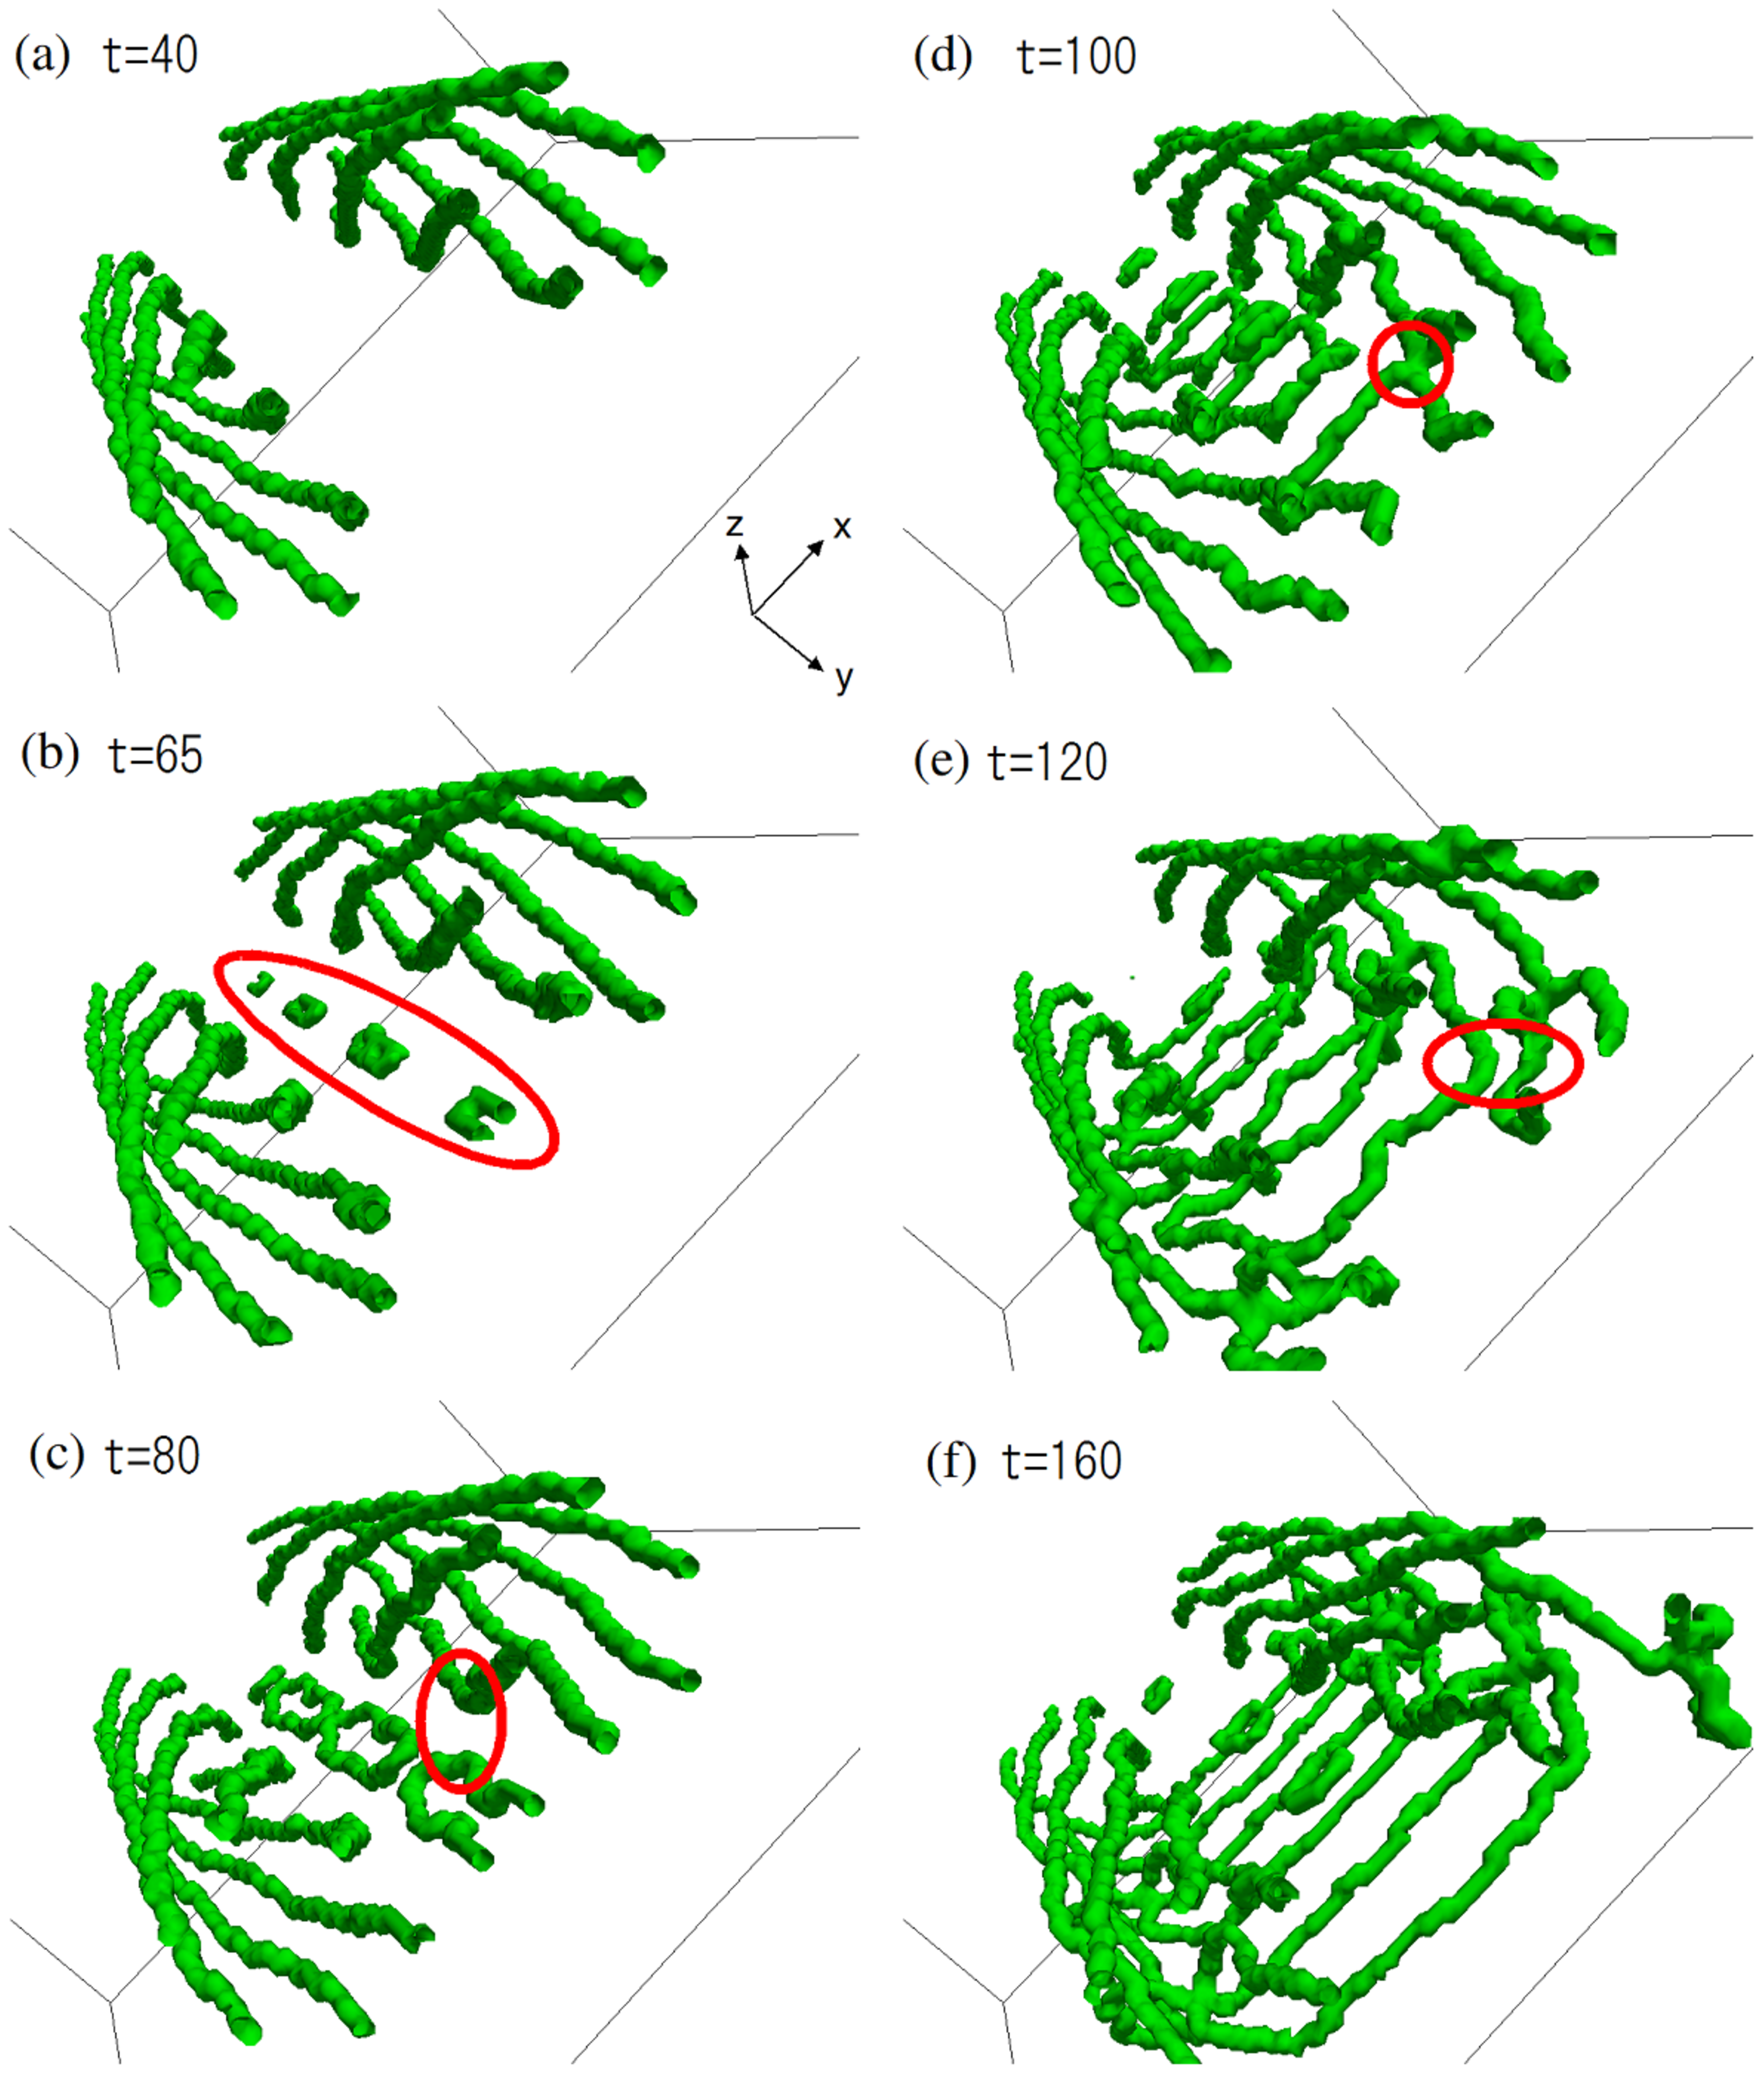
\includegraphics[width=15cm]{bundle_core.eps}
				\caption{
					(a)--(f)は、スケール間のカスケード過程の詳細について、
					図.~\ref{FIG:SETUP}の別の角度から見た渦芯のダイナミクスを示す。
                    大スケールの渦バンドルが回転しながら移動し、(b)で渦バンドルの
                    伸張により、局所的に音速を超える部分から
                    小さな渦輪が生成される。
                    (c)で小さな渦輪が近傍の渦バンドルとリコネクションが起きる。
                    (d)--(f)で低波数の渦バンドルと直交した配置で小スケールの渦バンドルが生成し
                    渦度のカスケードが起きる。
                    このダイナミクスにより、同時にエネルギースペクトルも大スケールから小スケールへ
                    カスケードしていると示唆される。
				}
				\label{FIG:bndl_core}
			\end{figure}
			図.~\ref{FIG:bndl_core}ではその過程の詳細を示す。図.~\ref{FIG:bndl_core} (b)の様に大スケールの渦バンドルの間で、
			渦バンドルの伸張によって周囲の速度が局所的に臨界速度を超え、その領域の場所から小さな渦輪が生成される。
			図.~\ref{FIG:bndl_core}(c)から(e)の過程では、生成された渦輪が引き伸ばされ
			大スケールの渦バンドルの渦芯に接触し、渦芯のリコネクションが起こる。
			リコネクションの後は、図.~\ref{FIG:bndl_core} (f)の様な
			大スケールの渦バンドルとの間に、はしご状の構造の小スケールの渦バンドルが生成される。
			このように渦芯のダイナミクスが可視化されることで、
            大スケールの渦バンドルから小スケールへのカスケード過程が明らかとなった。
			\begin{figure}[H]
				\centering
				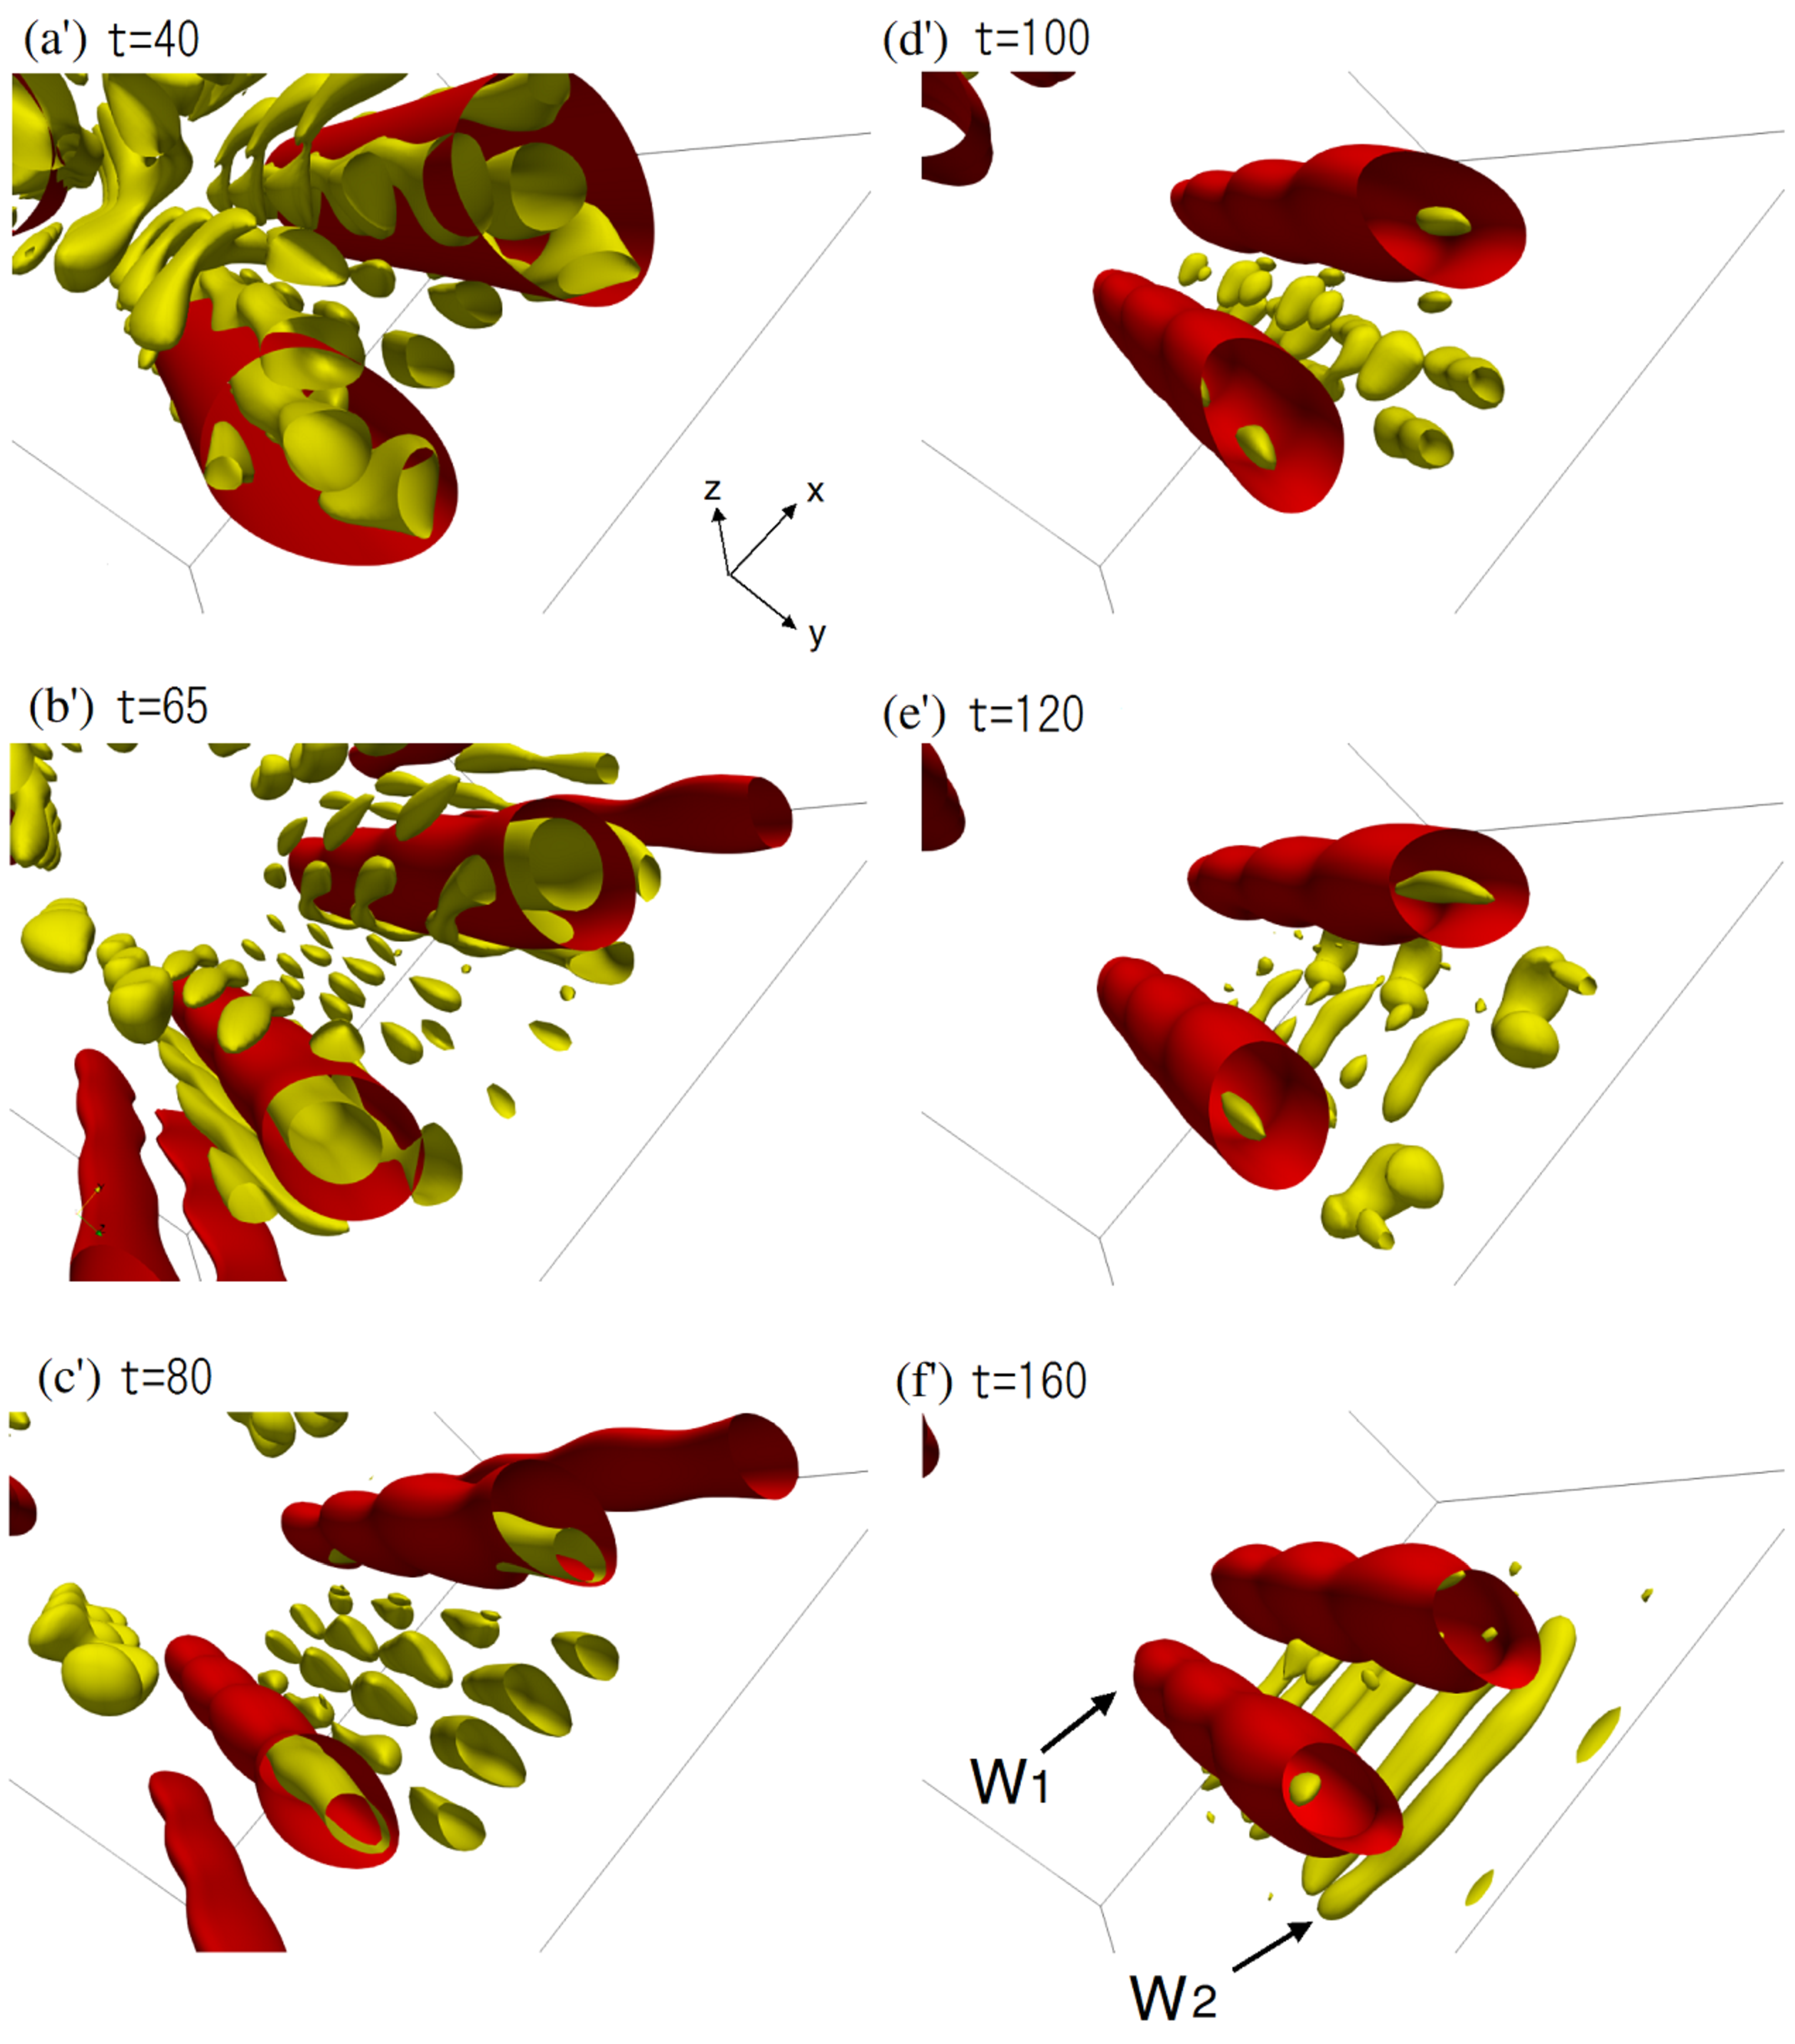
\includegraphics[width=15cm]{bundle_vor.eps}
				\caption{
					(a$'$)--(f$'$)は図.~\ref{FIG:bndl_core}の渦度分布について、
                    波数スペクトルのバンドパスフィルターで$|\bm{W}_1|$と
					$|\bm{W}_2|$に抽出した等渦度面。
                    時間発展により大スケールの渦度から小スケールの渦度がカスケード生成しているが確認できる。
                    $\bm{W}_1$のバンドパスの範囲は$4/\sqrt{2}\leq |\bm{k}| < 4\sqrt{2}$、
                    $\bm{W}_2$のバンドパスの範囲は$7/\sqrt{2}\leq |\bm{k}| < 7\sqrt{2}$である。 
				}
				\label{FIG:bndl_vor}
			\end{figure}
			図.~\ref{FIG:bndl_vor} (a$'$)から(f$'$)はバンドパスフィルターにより抽出された
			$|\bm{W}_1|$と$|\bm{W}_2|$の等渦度面である。
            $|\bm{W}_1|$、$|\bm{W}_2|$は、
            渦度ベクトルの絶対値をとった渦度の大きさ
            \begin{eqnarray}
                |\bm{W}_1| & = & \sqrt{W_{1_x}^2+W_{1_y}^2+W_{1_z}^2}
                \\
                |\bm{W}_2| & = & \sqrt{W_{2_x}^2+W_{2_y}^2+W_{2_z}^2}
            \end{eqnarray}
            をあらわす。
			バンドパスフィルターの$|\bm{W}_1|$の波数の範囲は
			$4/\sqrt{2} \leq |\bm{k}| < 4\sqrt{2}$、
			$|\bm{W}_2|$は
			$7/\sqrt{2} \leq |\bm{k}| < 7\sqrt{2}$である。
			大スケールの渦度分布として$\bm{W}_1$、小スケールとして$\bm{W}_2$を観測する。
			図.~\ref{FIG:bndl_vor} (a$'$)では時刻$t=40$で$\bm{W}_1$の周囲に渦度$\bm{W}_2$が
			生成しはじめる。その後、$\bm{W}_1$の間の$\bm{W}_2$が引き伸ばされ、渦度$\bm{W}_1$の管状の
			等渦度面が細くなっていく。$t \lesssim 120$の期間では渦度$\bm{W}_2$は
			断片的に分布しているが、$t=160$の$\bm{W}_2$では図.~\ref{FIG:bndl_vor} (f$'$)に示す様な管状に成長し、
			$\bm{W}_1$に対して直交した配置をとる。
			この結果はエネルギーカスケードによる、大スケールの構造が小スケールの構造を形成する
			過程のダイナミクスを明らかにしている。
			以上の渦バンドルの伸張を起因とした同様のダイナミクスは古典流体でも発見されている
			~\cite{Goto2, Melander, Kerr2}。
			\begin{figure}[H]
				\centering
				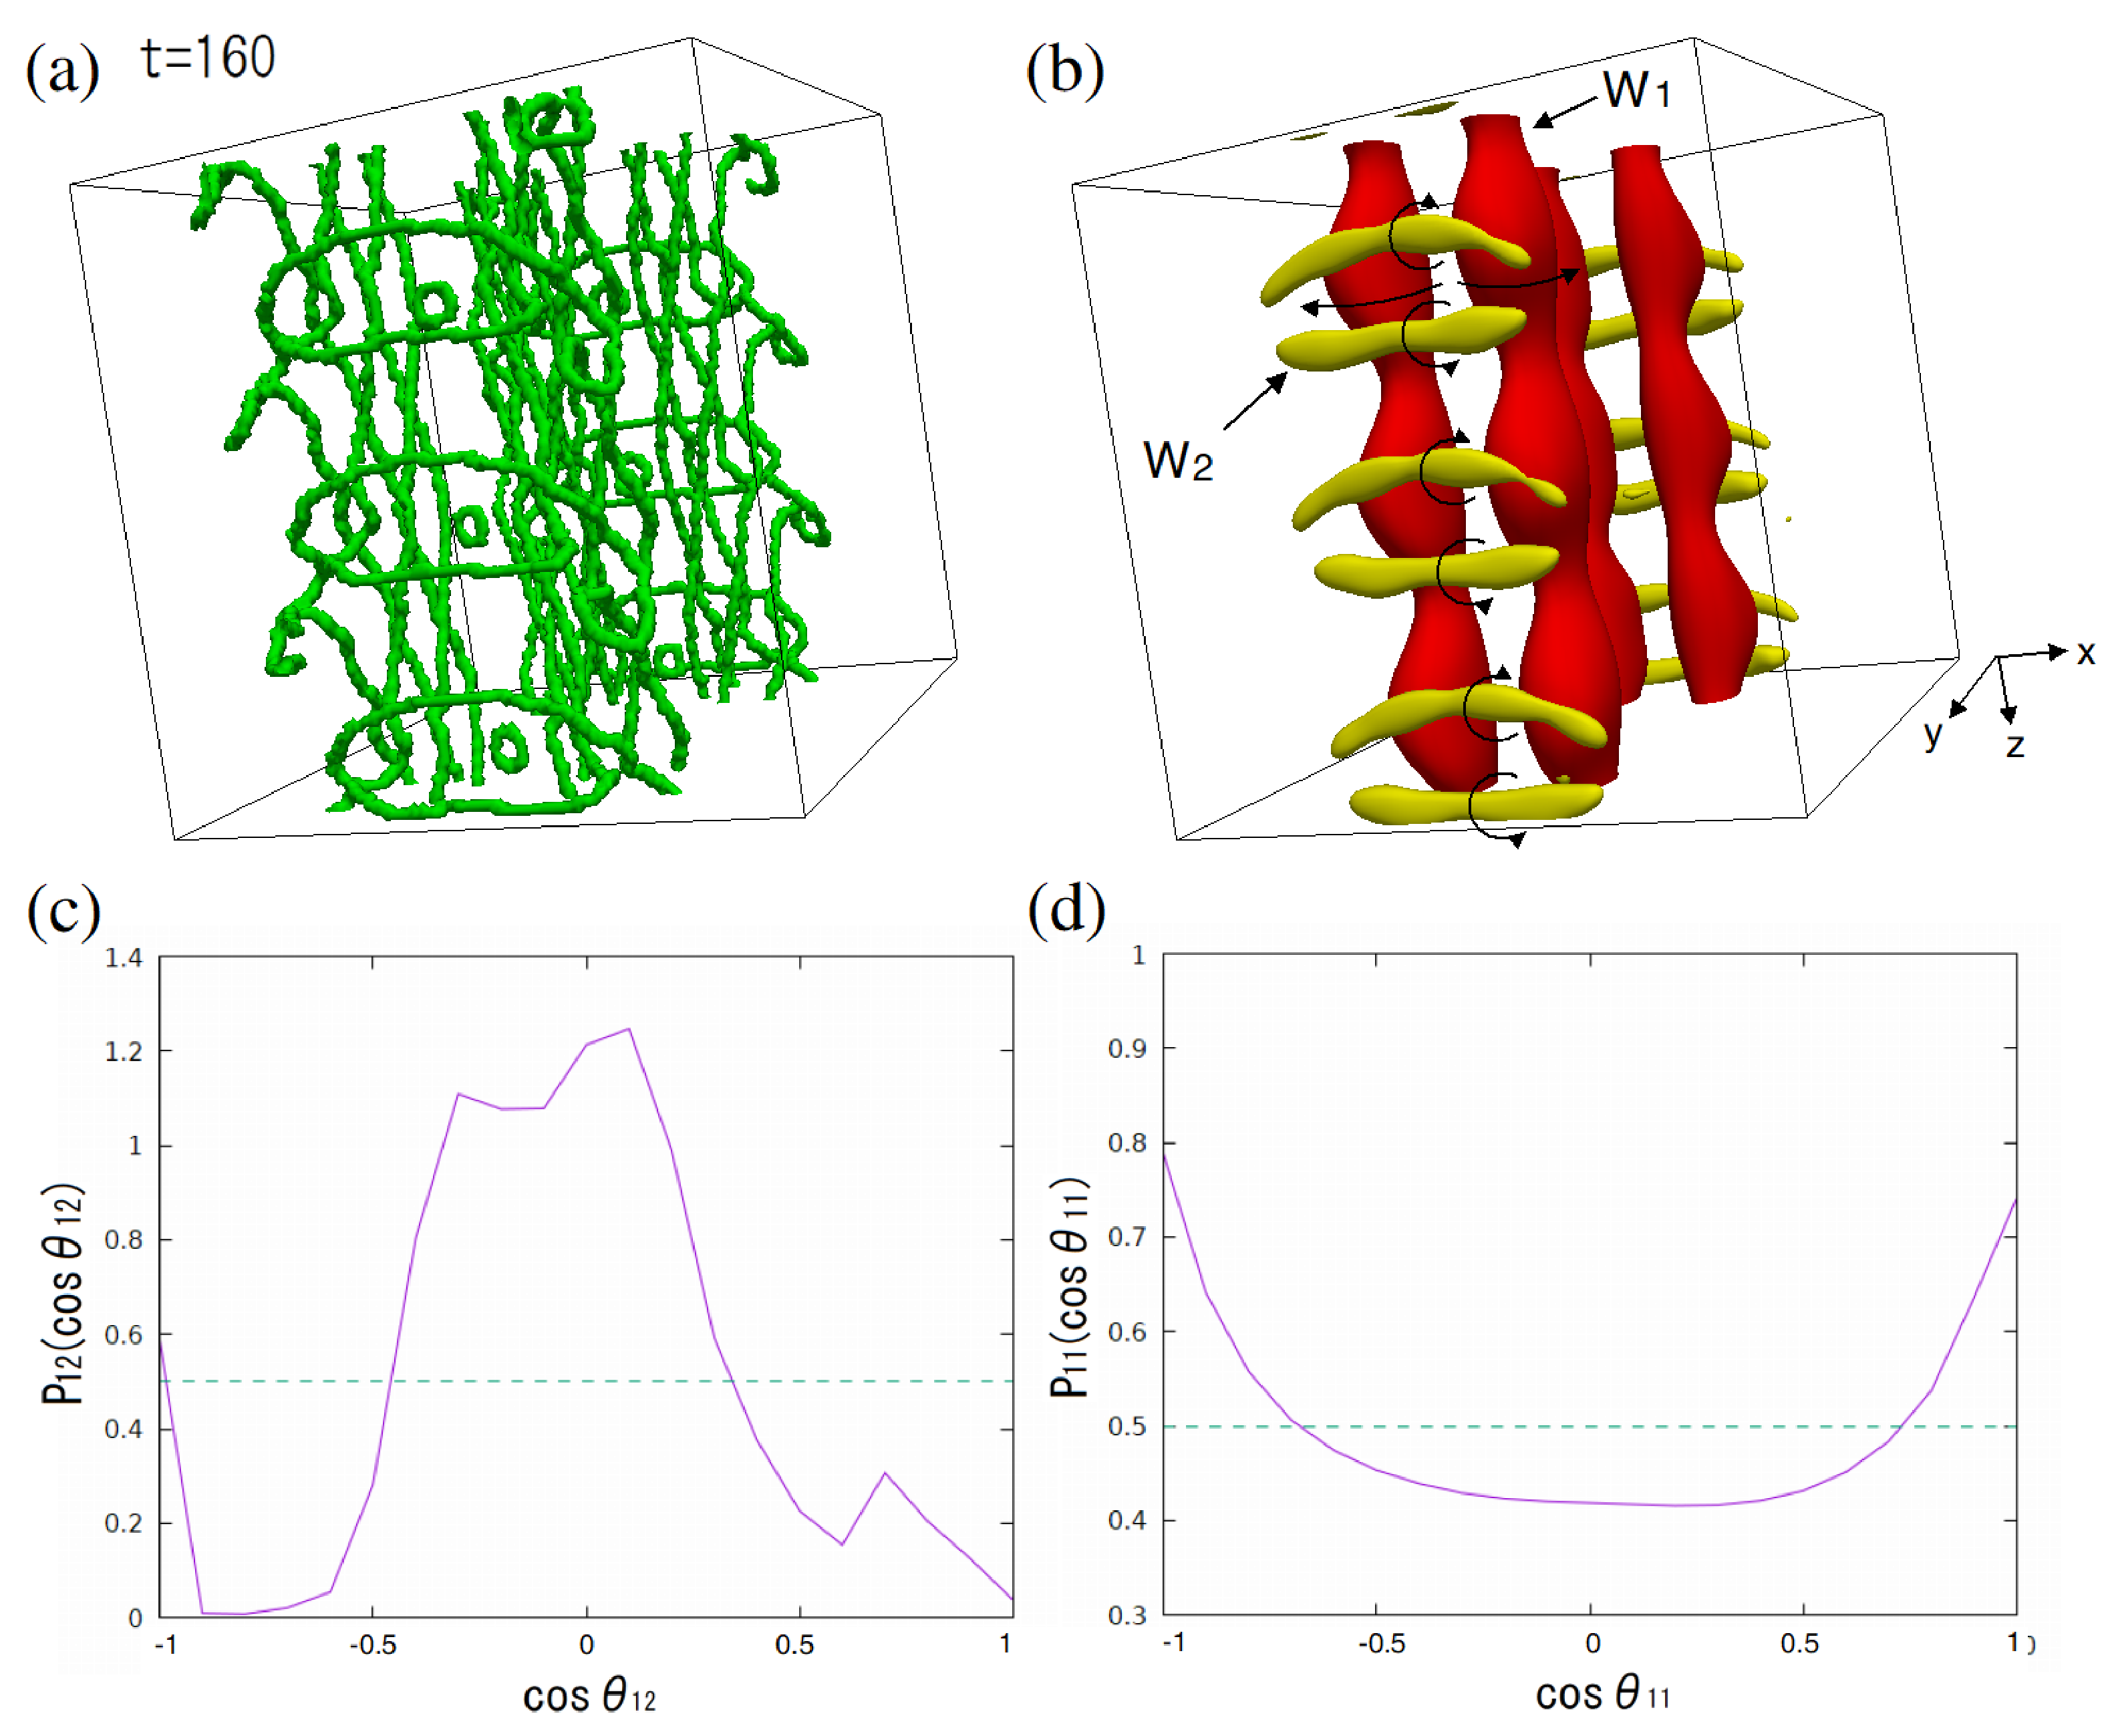
\includegraphics[width=15cm]{fig13.eps}
				\caption{
                    図.~\ref{FIG:bndl_vor}について、(a)は$t=160$の時刻の渦芯、(b)はその等渦度面を示す。
                    (b)の図から目視でも、大スケールの渦度$|\bm{W}_1|$(赤色)とそれから生成された
                    小スケールの渦度$|\bm{W}_2|$(黄色)が直交した位置関係であることがわかる。
                    (c)は大スケールの渦度$\bm{W}_1(\bm{r})$と小スケールの渦度$\bm{W}_2(\bm{r}+\Delta\bm{r})$の
                    角度分布$\theta_{12}$。
                    (d)は隣り合う大スケールの渦度の対$\bm{W}_1(\bm{r})$と$\bm{W}_1(\bm{r}+\Delta\bm{r})$の
                    角度分布$\theta_{11}$。
                    角度分布を相関関数を用いて算出した(c)の直交性、(d)の反平行性が確認できる。
                    算出範囲$|\Delta\bm{r}|$は、等渦度面がある$48 \leq |\Delta\bm{r}| < 50$を選ぶ。
                    (b)の等渦度面の図では、それぞれの渦度の回転方向を記している。
                    また、大スケールの渦度$|\bm{W}_1|$が渦伸張により渦バンドルの直径が大きな部分と
                    小さな部分が見られる。直径が大きな部分では周速度が速く、音速をこえると局所的に
                    渦が生成される。
				}
				\label{FIG:orthant}
			\end{figure}
			図.~\ref{FIG:orthant} (a)と(b)では、図.~\ref{FIG:bndl_core} (f)と 図.~\ref{FIG:bndl_vor} (f$'$)を別の角度から見たときの、
			はしご状に形成された渦芯と、同じ時刻の渦度分布を示す。図.~\ref{FIG:orthant} (b)では
			渦管${W}_1$の対と、
			生成された隣接する小スケールの渦管${W}_2$の対それぞれ反平行の回転であることがわかる。
			渦管について角度の関係性を定量化するため
			図.~\ref{FIG:orthant} (b)の状態での、
			それぞれの角度相関$\cos \theta_{12}$と$\cos \theta_{11}$を算出したものを、
			図.~\ref{FIG:orthant} (c)と(d)に示す。
			~(\ref{eq:ORTH}) と(\ref{eq:ANTI})を用いるときの距離$|\Delta\bm{r}|$は
			$48$--$50$の範囲内を基準にした。
			角度分布$P_{12}(\cos \theta_{12})$では、$\cos \theta_{12}=0$にピークを示し、
			大小スケール間の渦度 $\bm{W}_1(\bm{r})$ と $\bm{W}_2(\bm{r}+\Delta\bm{r})$で互いに
			直交性の傾向である。
			角度分布$P_{11}(\cos\theta_{11})$では、$\cos\theta_{11}=-1$にピークを示し、
			同じスケール間の渦度 $\bm{W}_1(\bm{r})$ と $\bm{W}_1(\bm{r}+\Delta\bm{r})$で互いに
			反平行性の傾向である。
            また、$\cos\theta_{11}=1$のピークは、自身が太さのある渦バンドルを持つために同じ方向の渦度ベクトルとしてあらわれている。
			以上の結果から、大スケールの反平行渦から直交した小スケールの渦がカスケード生成する過程は、
            古典流体の先行研究と同等であることがわかった
			~\cite{Goto2}。

		    \subsection{量子乱流における渦度分布の階層構造}
            \label{s:distributions}
			    \begin{figure}[H]
				    \centering
				%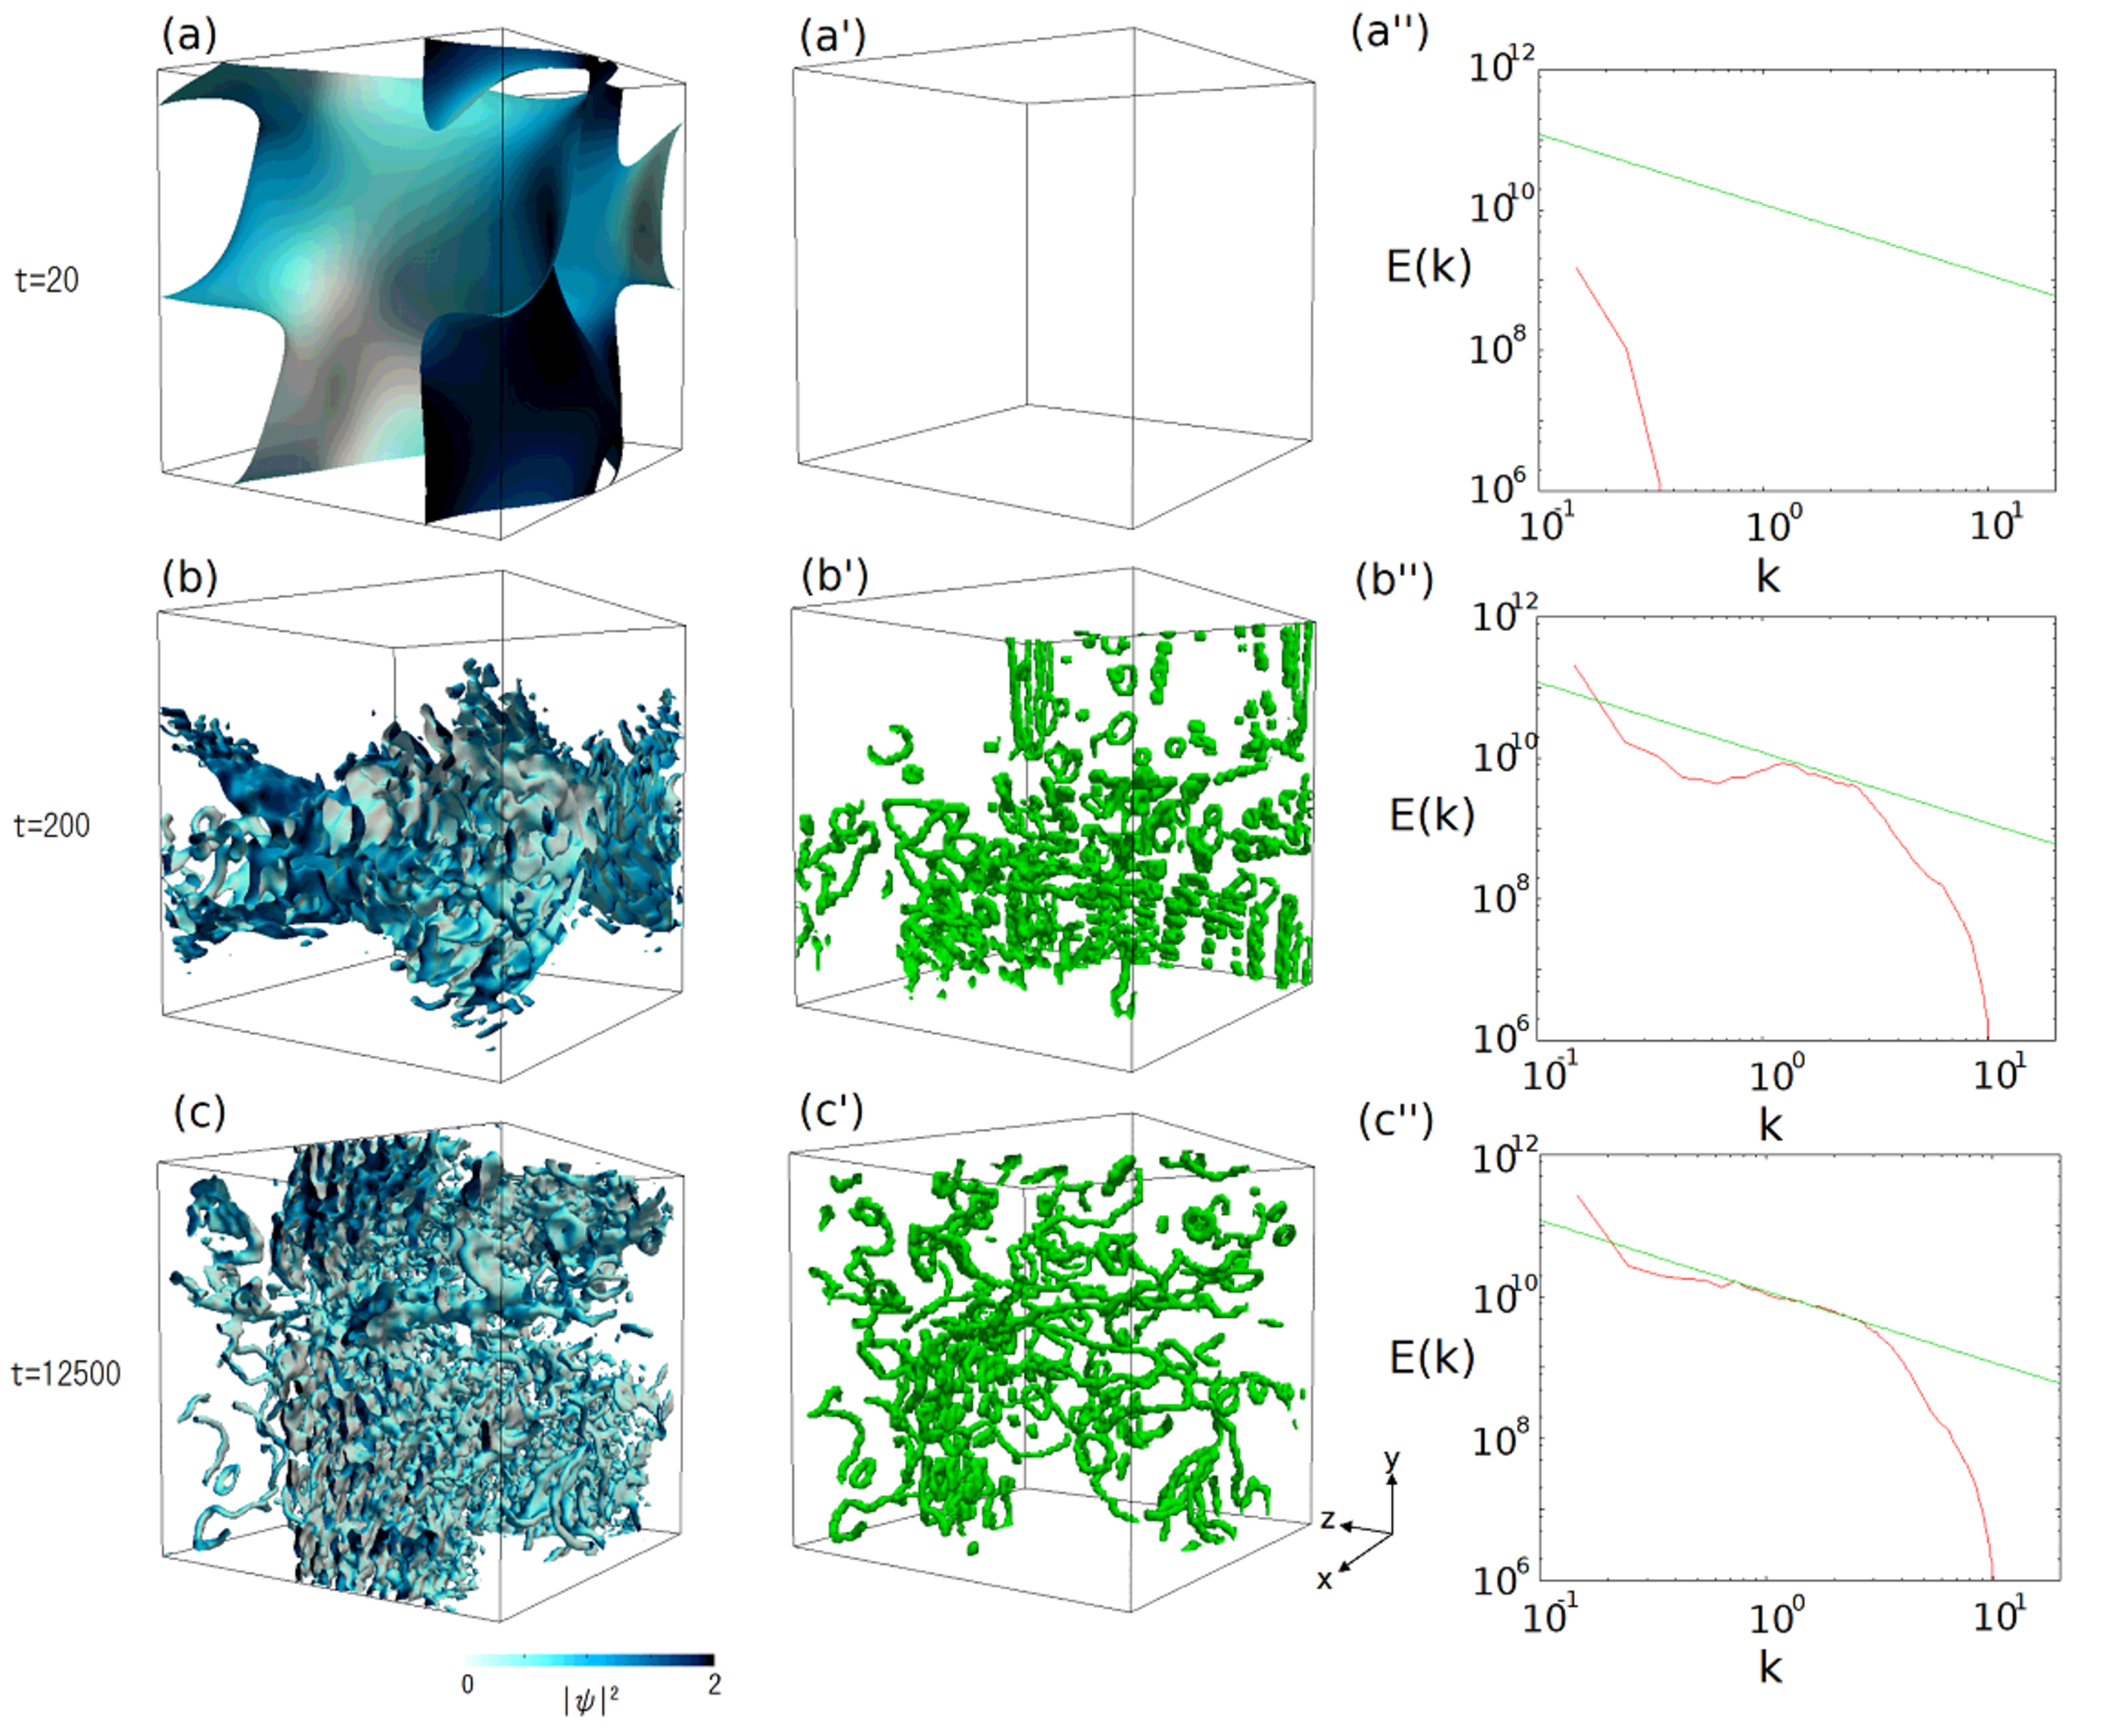
\includegraphics[width=17cm]{fig14.eps}
				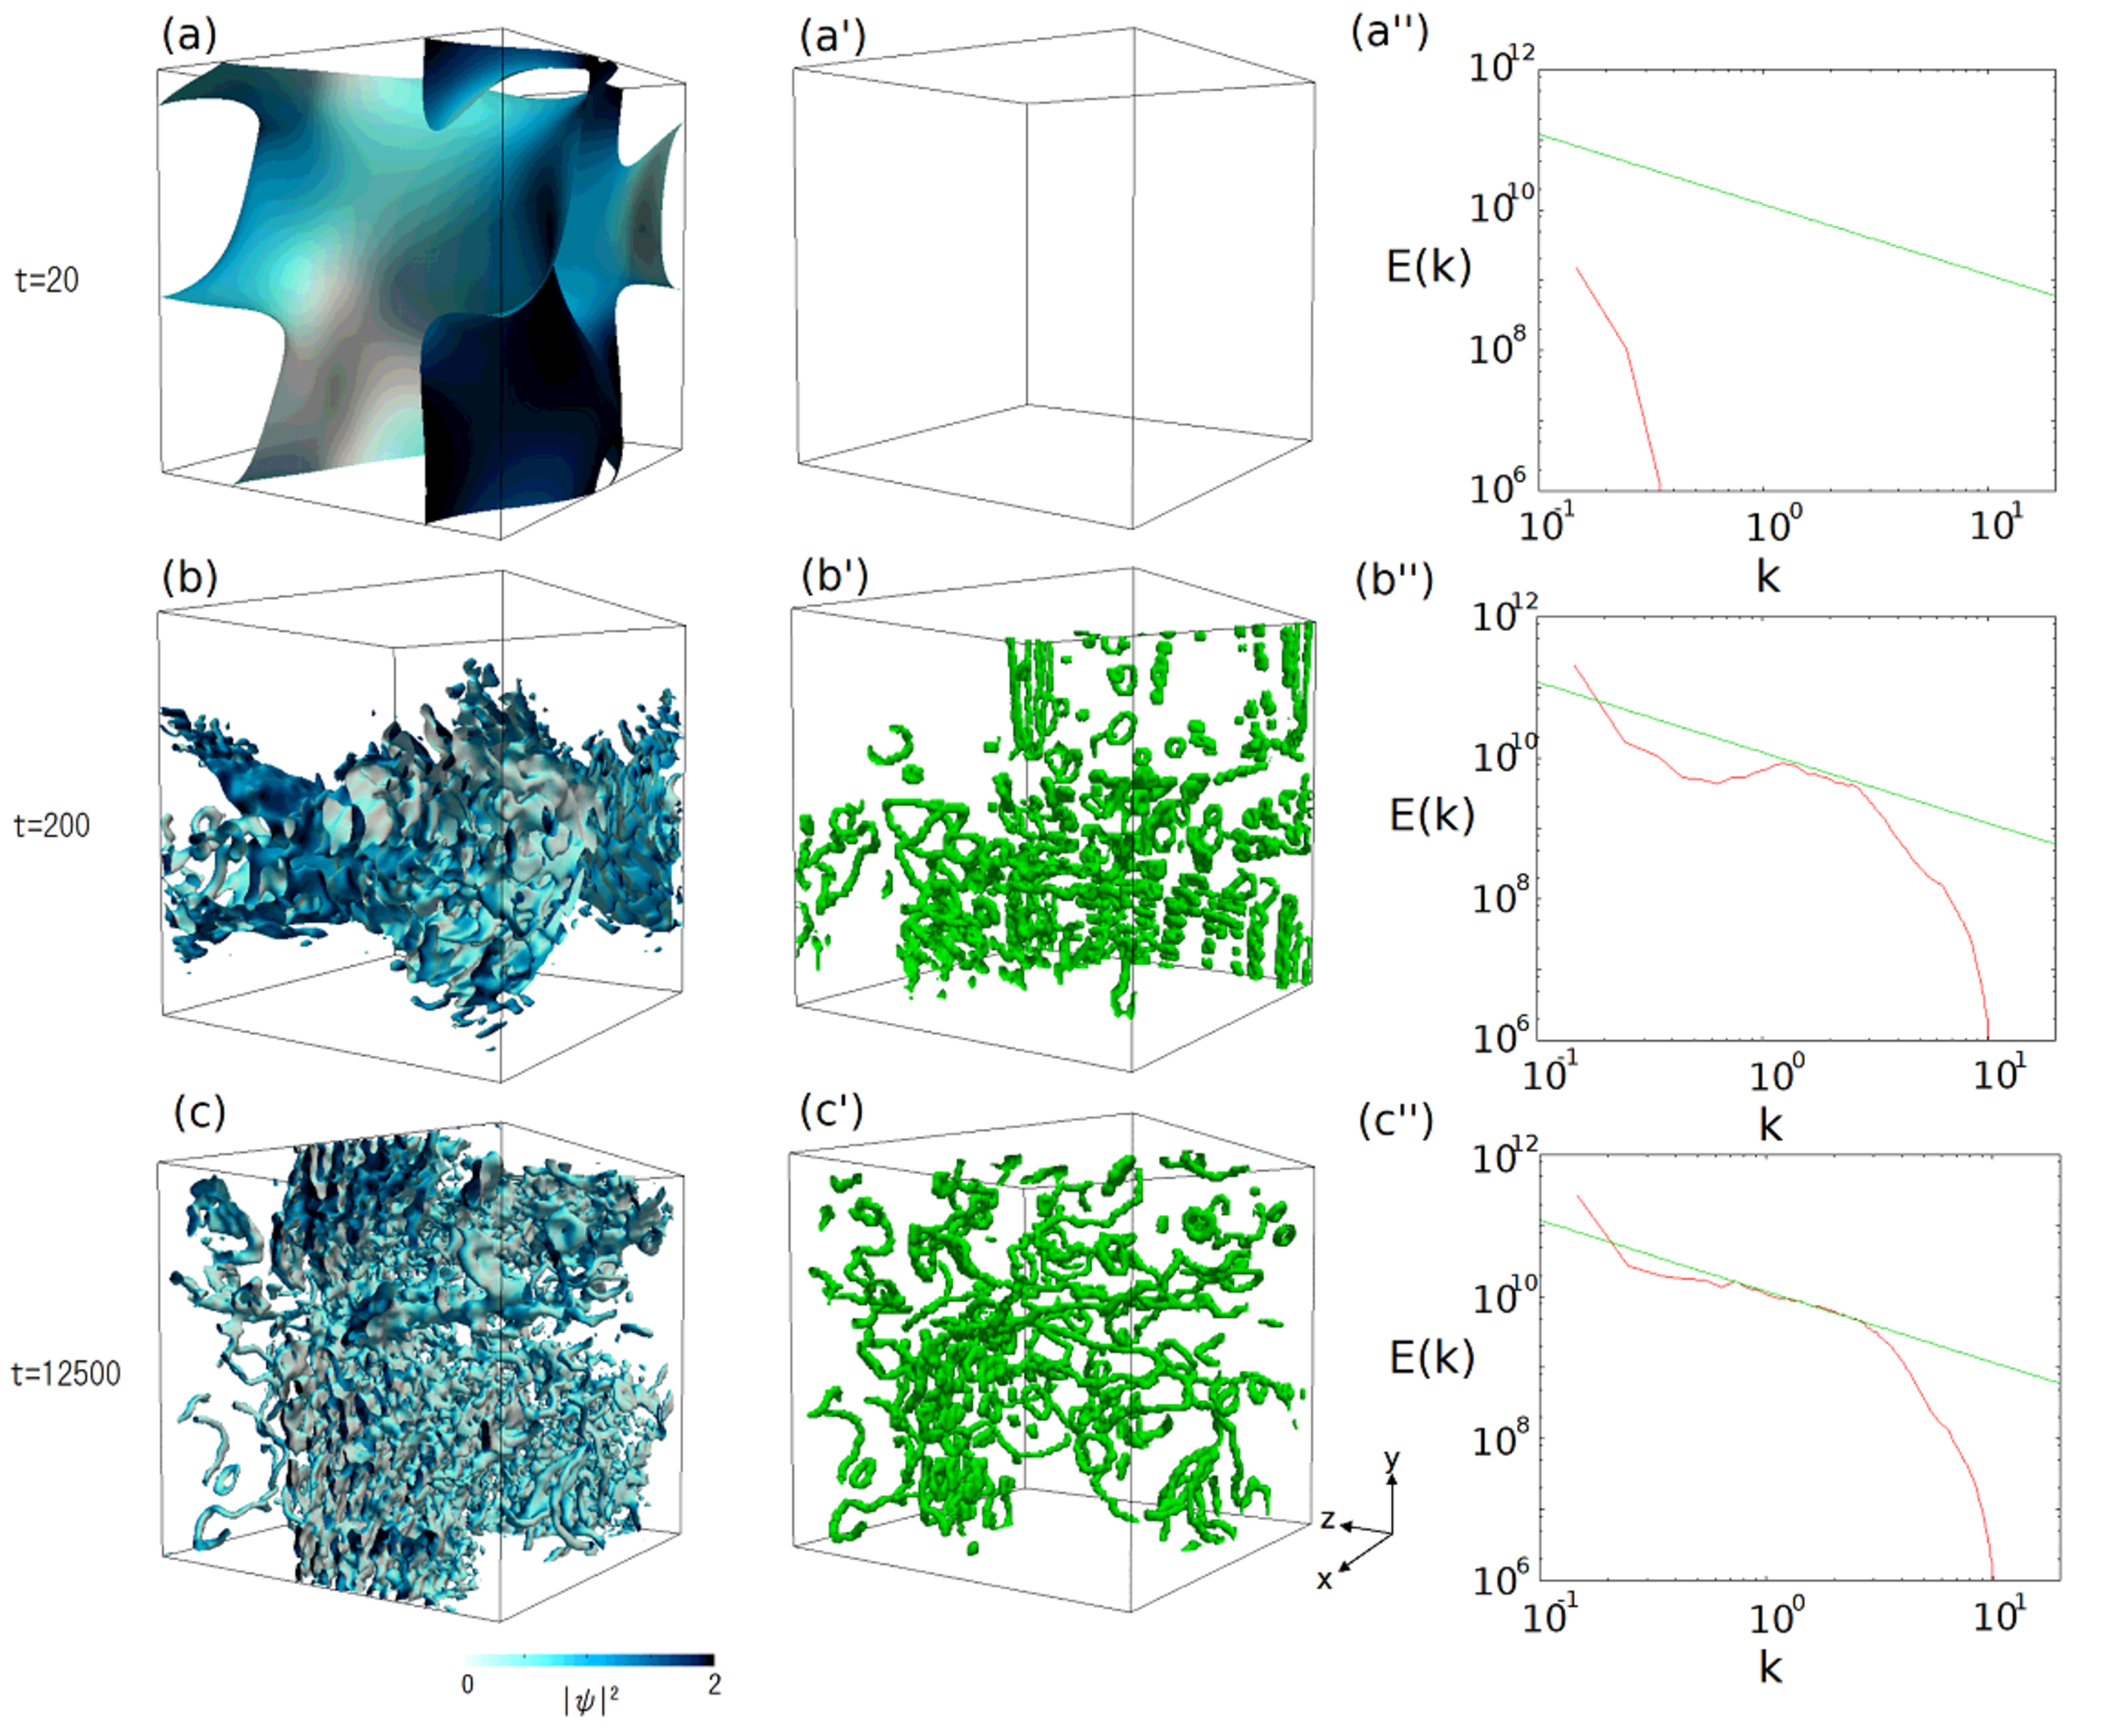
\includegraphics[width=16cm]{fig14.eps}
				\caption{
                    $128^3$の三次元空間で超流動体が定常乱流に至るまでの時間発展の様子。
                    (a)--(c)は等密度面$|\tilde{\psi}|^2$、
                    (a$'$)--(c$'$)は同時刻の渦芯、(a$''$)--(c$''$)は同時刻のエネルギースペクトル$E(k)$を示す。
                    乱流を発生させる外力のランダムポテンシャルは
					$U(\bm{r}, t)$で、~\ref{s:random}(B)の~(\ref{eq:RANDOM})のパラメータとして、
					$\kappa=0.05, A_0=0.5$, and $l=8\pi $である。
                    乱流のエネルギースペクトルは、(c$''$)の$-5/3$べき乗のコルモゴロフ則に到達する。
					%See the Supplemental Material for a movie of the dynamics
					%in (a$'$)--(c$'$)~\cite{SM}.
				}
				\label{FIG:TURB}
			\end{figure}
			~\ref{s:nucleation}節の方法と結果をもとに、量子流体の三次元空間中でランダムポテンシャルによる外力を与え、
            発達した一様等方な定常乱流について同様の調査を行った。
			式~(\ref{eq:NGPE})に対し、
			$U(\bm{r},t)$に~\ref{s:random}(B)で示す
            ランダムポテンシャルを与え、その時間発展を数値的にもとめる。
			この系は$L^3=128^3$の三次元空間である。
			図.~\ref{FIG:TURB}の(a)--(c)は等密度面$|\tilde\psi|^2$、
            (a$'$)--(c$'$)は同じ時刻の渦芯プロファイル、
			(a$''$)--(c$''$)は同じ時刻のエネルギースペクトル$E(k)$
            である。

			低波数のランダムポテンシャルにより、量子流体に対して大スケールの
			外力がランダムに働く。図.~\ref{FIG:TURB}(a)の$t=20$あたりから密度にその影響が見えはじめる。
            この段階では図.~\ref{FIG:TURB}(a$'$)の量子渦がまだ生成されていない。
			大スケールの流れから
            発達した乱流になると、低波数から高波数の方向へエネルギーがカスケードする。
			図.~\ref{FIG:TURB}(a$''$)のエネルギースペクトルは低波数の領域から現れ始め、
            時間発展に伴って図.~\ref{FIG:TURB}(b$''$)の時刻$t \geq 200$の定常状態では
            $E(k) \propto k^{-5/3}$のコルモゴロフ則のエネルギースペクトルを示し、
			発達した乱流の定常状態となる。
			\begin{figure}[H]
				\centering
				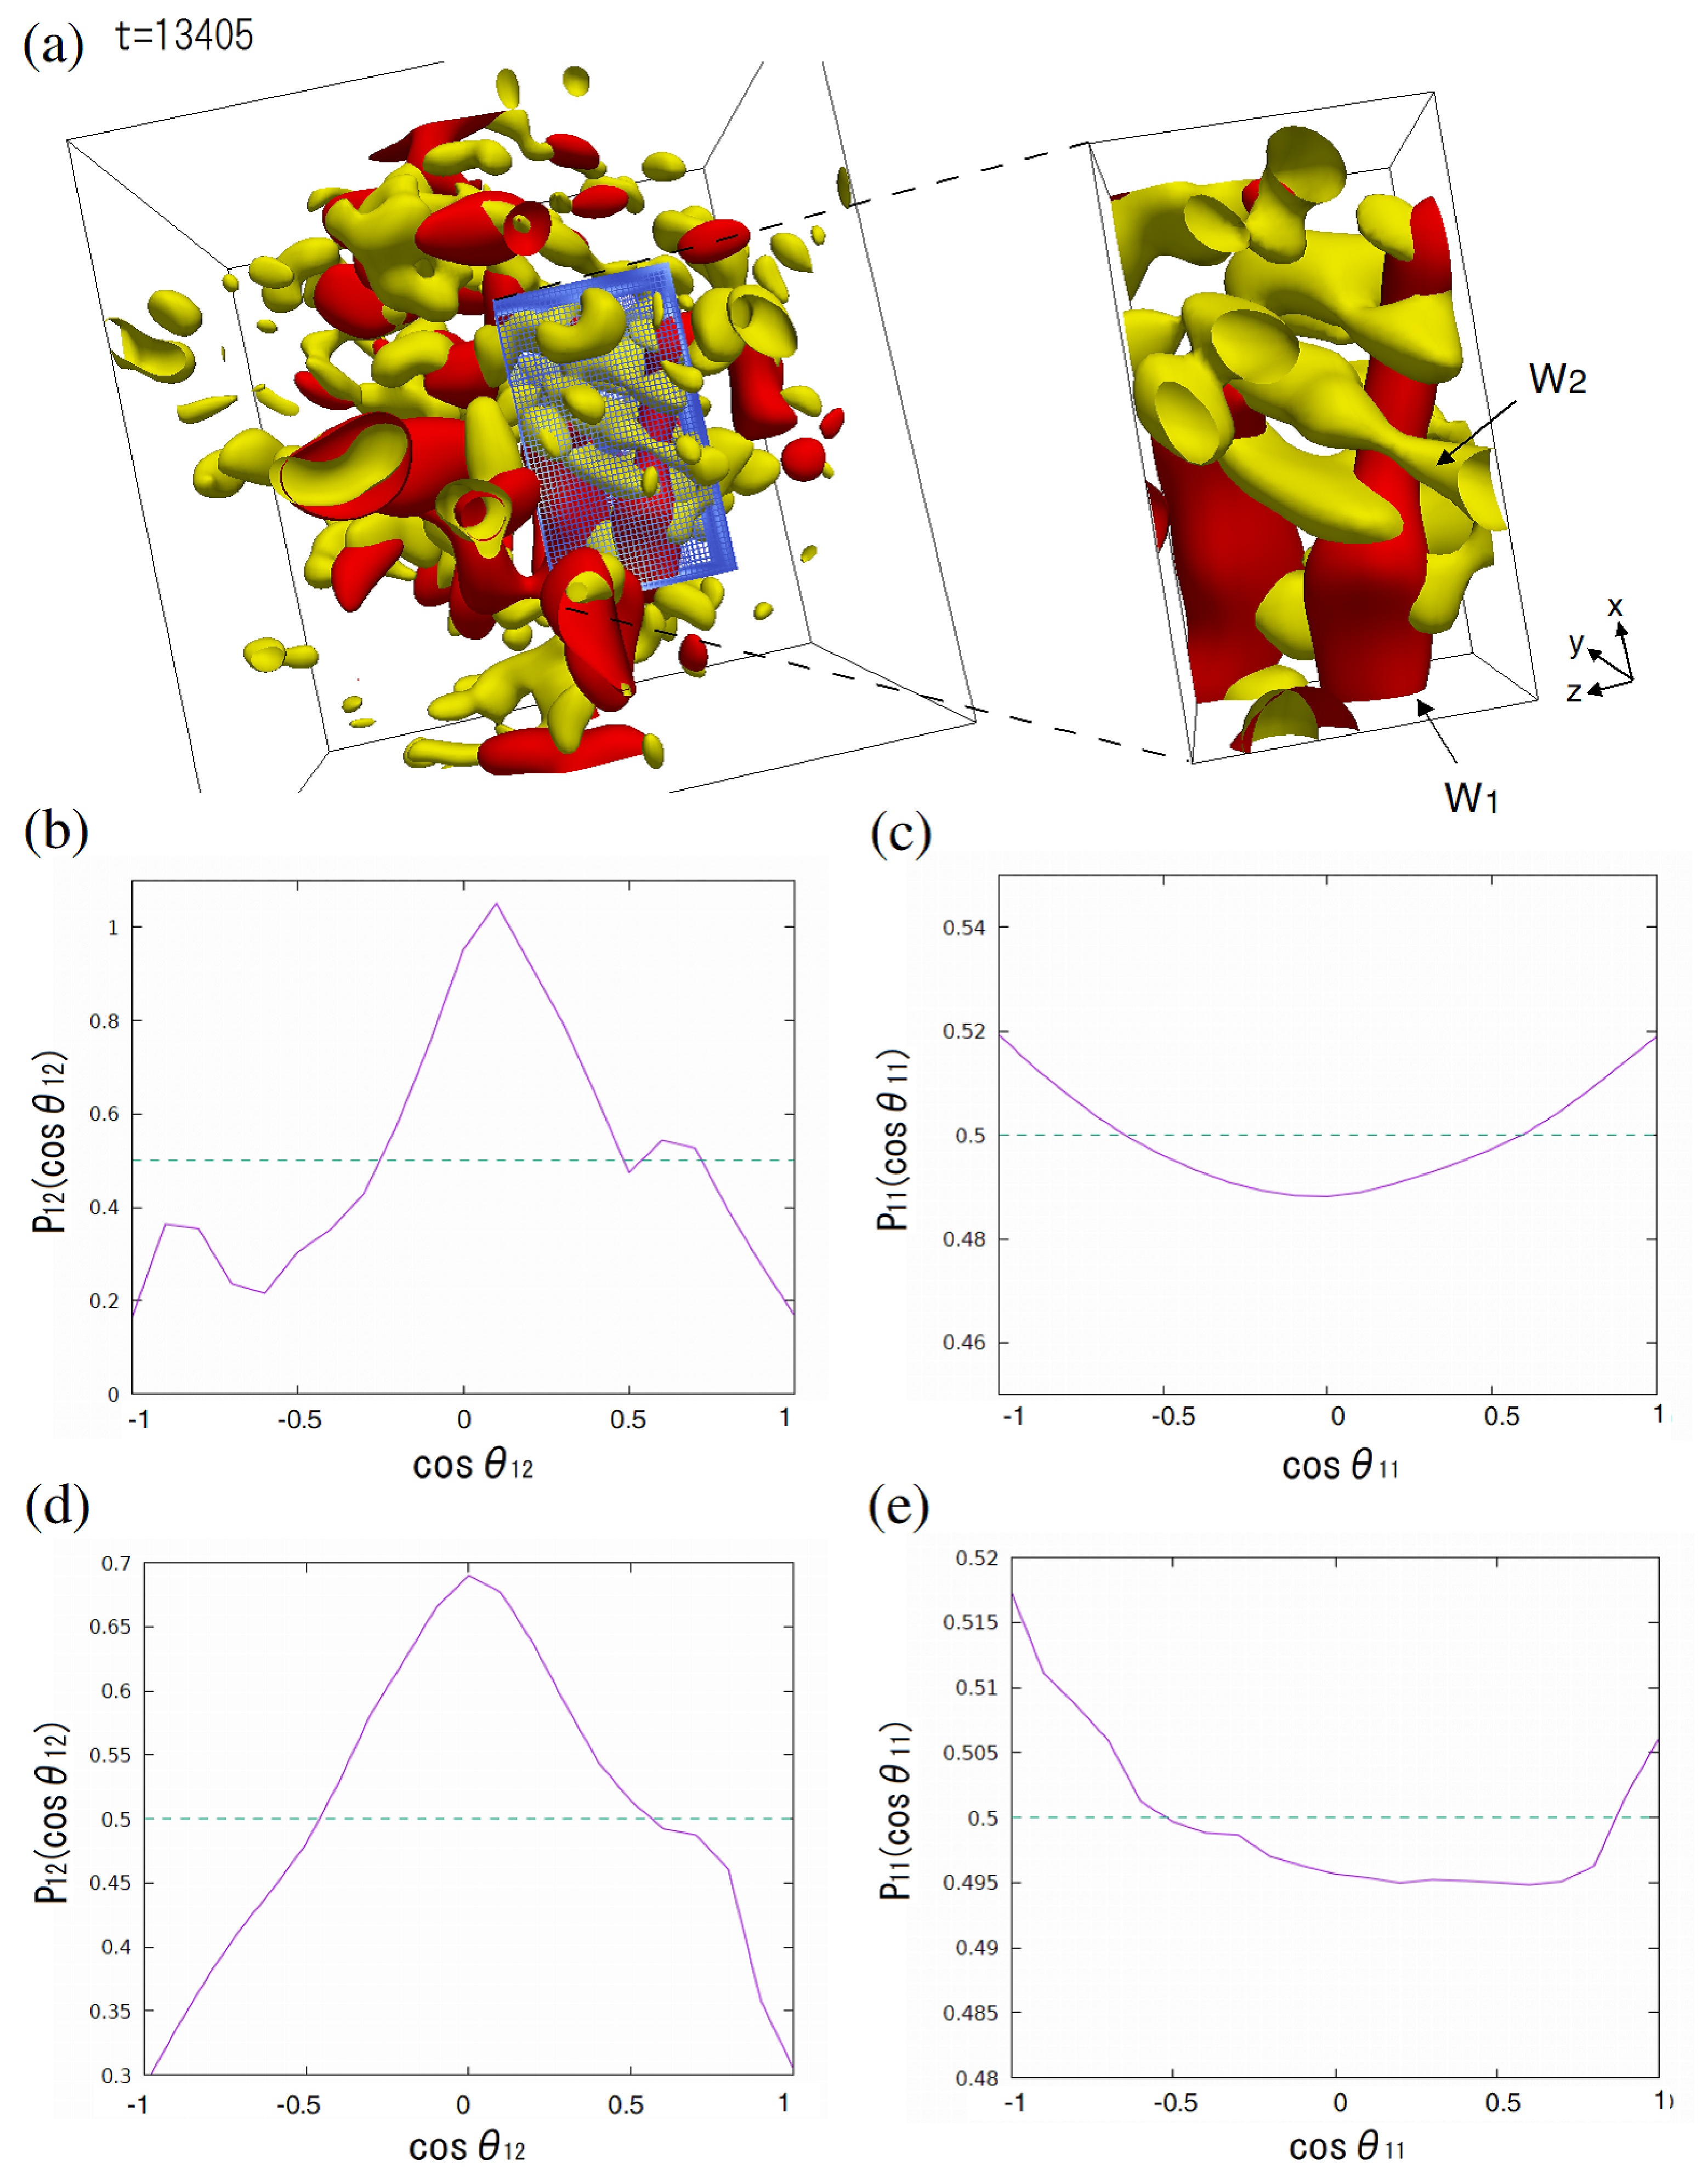
\includegraphics[width=15cm]{fig15.eps}
				\caption{
                    図.~\ref{FIG:TURB}で示す発達した乱流の渦度分布。
                    (a)は時刻$t=13405$の大スケールの渦度分布$|\bm{W}_1|$と小スケールの
                    渦度分布$|\bm{W}_2|$。右側の拡大図は、フーリエ変換による波数スペクトルの
                    バンドパスフィルターにより抽出した$\bm{W}_1$と$\bm{W}_2$の大小の渦度分布が直交して
                    配置されているのが目視でも確認できる。
                    (b)は同じ時刻における、大スケールの渦度$\bm{W}_1(\bm{r})$と小スケールの渦度$\bm{W}_2(\bm{r}+\Delta\bm{r})$の
                    角度分布$\theta_{12}$。
                    (c)は同じ時刻における、隣り合う大スケールの渦度の対$\bm{W}_1(\bm{r})$と$\bm{W}_1(\bm{r}+\Delta\bm{r})$の
                    角度分布$\theta_{11}$。
                    より高い信憑性を得るため、
                    (d)と(e)は、それぞれ$13000 \leq t < 14000$の時間$1000$の間を平均して得られた角度分布。
                    角度分布を相関関数を用いて算出した(b)、(d)の直交性、(c)、(e)の反平行性が確認できる。
                    角度分布$P_{11}$と$P_{12}$は$128^3$全空間から算出した。
					%See the Supplemental Material for the dynamics and rotating view of (a)~\cite{SM}.
				}
				\label{FIG:antipara}
			\end{figure}
			ここで大スケール渦から小スケール渦の生成に伴い、
			エネルギーが波数スペクトル間でどのように伝達しているか、
            ~\ref{s:nucleation}節と同じ方法で乱流中の渦度分布を
			$\bm{W}_1$と$\bm{W}_2$にバンドパスフィルターで抽出し分析を行う。
			図.~\ref{FIG:antipara}(a)では、時刻$t=13405$のときの$|\bm{W}_1|$
			と$|\bm{W}_2|$の等渦度面を示す。$\bm{W}_1$と$\bm{W}_2$の各スケールの
			抽出条件は図.~\ref{FIG:orthant}と同じく、それぞれ大スケール渦は$\bm{W}_1$、
			小スケール渦は$\bm{W}_2$に対応する。
			図.~\ref{FIG:antipara}(a)の右図は、青枠の範囲を拡大したものである。
			その拡大図のみ注視すると$\bm{W}_1$の渦管の並行にあるペアと、
			その$\bm{W}_1$と直交した$\bm{W}_2$の渦管がはっきりと確認できる。
			ちょうど図.~\ref{FIG:antipara}(a)にある反平行渦配置での構成に相当する。
			それに反して、図.~\ref{FIG:antipara}(a)そのものは、ランダムポテンシャルにより
			形成された乱雑な構造のため目視からその特徴はわからない。
			そこで~\ref{s:nucleation}節と同様に、
            式~(\ref{eq:ORTH})と式~(\ref{eq:ANTI})で定義した方法を用いて、
			渦度$\bm{W}_1$と$\bm{W}_2$の角度分布$P_{12}$と$P_{11}$を
			抽出したものが、図.~\ref{FIG:antipara}(b)と図.~\ref{FIG:antipara}(c)に示す。
            図の結果から、ランダムポテンシャルにより誘起された乱流状態にもかかわらず、
            渦管の位置関係に重要な関係があることがわかる。
			$\bm{W}_1(\bm{r})$の渦管は角度分布$P_{12}(\cos \theta_{12})$が$\cos \theta_{12}=0$で
			ピークを示し、$\bm{W}_2(\bm{r} + \Delta \bm{r})$の渦管と直交性を示す傾向があり、
			角度分布$P_{11}(\cos \theta_{11})$が$\cos \theta_{11}=-1$でピークを示す、
			$\bm{W}_1(\bm{r} + \Delta \bm{r})$の渦管と反平行性を示す傾向がある。
			($\cos \theta_{11}=1$のピークは比較元である自身の$\bm{W}_1(\bm{r})$が渦バンドルの太さを持つためである。)
			この傾向が特定した偶発ではないことを確かめるため、$13000 \leq t  < 14000$の期間の
			時間平均の角度分布を計算した。
			ここで、ランダムポテンシャルが変動する代表的な時間周期は$\kappa^{-1}=20$で、
			目的の平均値を得るための時間幅はそれよりも十分長くとってある。
			図.~\ref{FIG:antipara}(d)と図.~\ref{FIG:antipara}(e)が示す時間平均は、
			それぞれ図.~\ref{FIG:antipara}(b)と図.~\ref{FIG:antipara}(c)の傾向と変わっていないことがわかる。
			したがって、定常的な乱流状態における渦度分布の角度関係は、
            ~\ref{s:nucleation}節の大スケール渦バンドル配置から時間発展させた場合のカスケードが、
            最初の手順で得られた結果と同様であることがわかった。
			以上の分析で、量子乱流においても、反平行の傾向を示す大スケール渦度の$\bm{W}_1$から
			直交性を示す小スケール渦度$\bm{W}_2$が生成される構造があることがわかった。
			これらの結果は動力学的な渦の伸張により大スケールから小スケールに向かってカスケード伝搬される
			エネルギーであることを示している。
			このことから$-5/3$べき乗のエネルギースペクトルのコルモゴロフ則を満足する
            量子乱流では、大スケールの渦バンドルから小スケールが生成される
            渦芯のリコネクションがランダムに起きていると推定できる。


		\section{むすび}
		\label{s:conclusions}
		本研究では超流動体の平均場近似を示すGP方程式の数値計算を用いて、
        量子流体における乱流中の渦度分布のカスケードを調査した。
        各スケールごとの渦度分布をバンドパスフィルターによって抽出し、
		研究を進めた。~\ref{s:nucleation}節では、反平行渦を配置したモデルを用いて、
		大スケールの反平行渦から、直交した小スケールの反平行渦がカスケード生成される過程があることを観測、調査した。
		これらの過程は量子化された渦輪の生成と再結合による誘起の繰り返しであることがわかった。
		~\ref{s:distributions}節では、一様に発達した乱流状態の系について同様の調査を行った。
		ランダムポテンシャルの外力により複雑な乱流状態である系においても、
        大小のスケールの渦度分布が同じようにカスケードすることがわかった。
		乱流の慣性領域において、カスケード過程の同スケール渦は、反平行に配置する傾向があり、
		またそこから生成される小スケール渦は、大スケール渦と直交する傾向がある。
		$-5/3$べき乗のエネルギースペクトルとなるコルモゴロフ則が成立している量子乱流の系において、
        この機構はエネルギーカスケードに
		重要な役割を果たしていると示唆される。
		本研究では、$\bm{W}_1$と$\bm{W}_2$の二つのスケール間での渦度分布を議論した。
		今後の展望としては、大規模な系でシミュレーションを行い、
		渦バンドルのより多段のスケール間で慣性領域のカスケード過程を調査する。


%%%%%%%%%%%% CHAPTER 4 %%%FORTH%%%%%%%%%%%%%%%%%%%%%%%%%%%%%%%%%%%%%%%%%%%%%%%%%
	\chapter{二成分系超流動体の定常乱流における流滴サイズとエネルギー注入率}
    \label{c:khscale}
        \begin{figure}[H]
            \centering
	        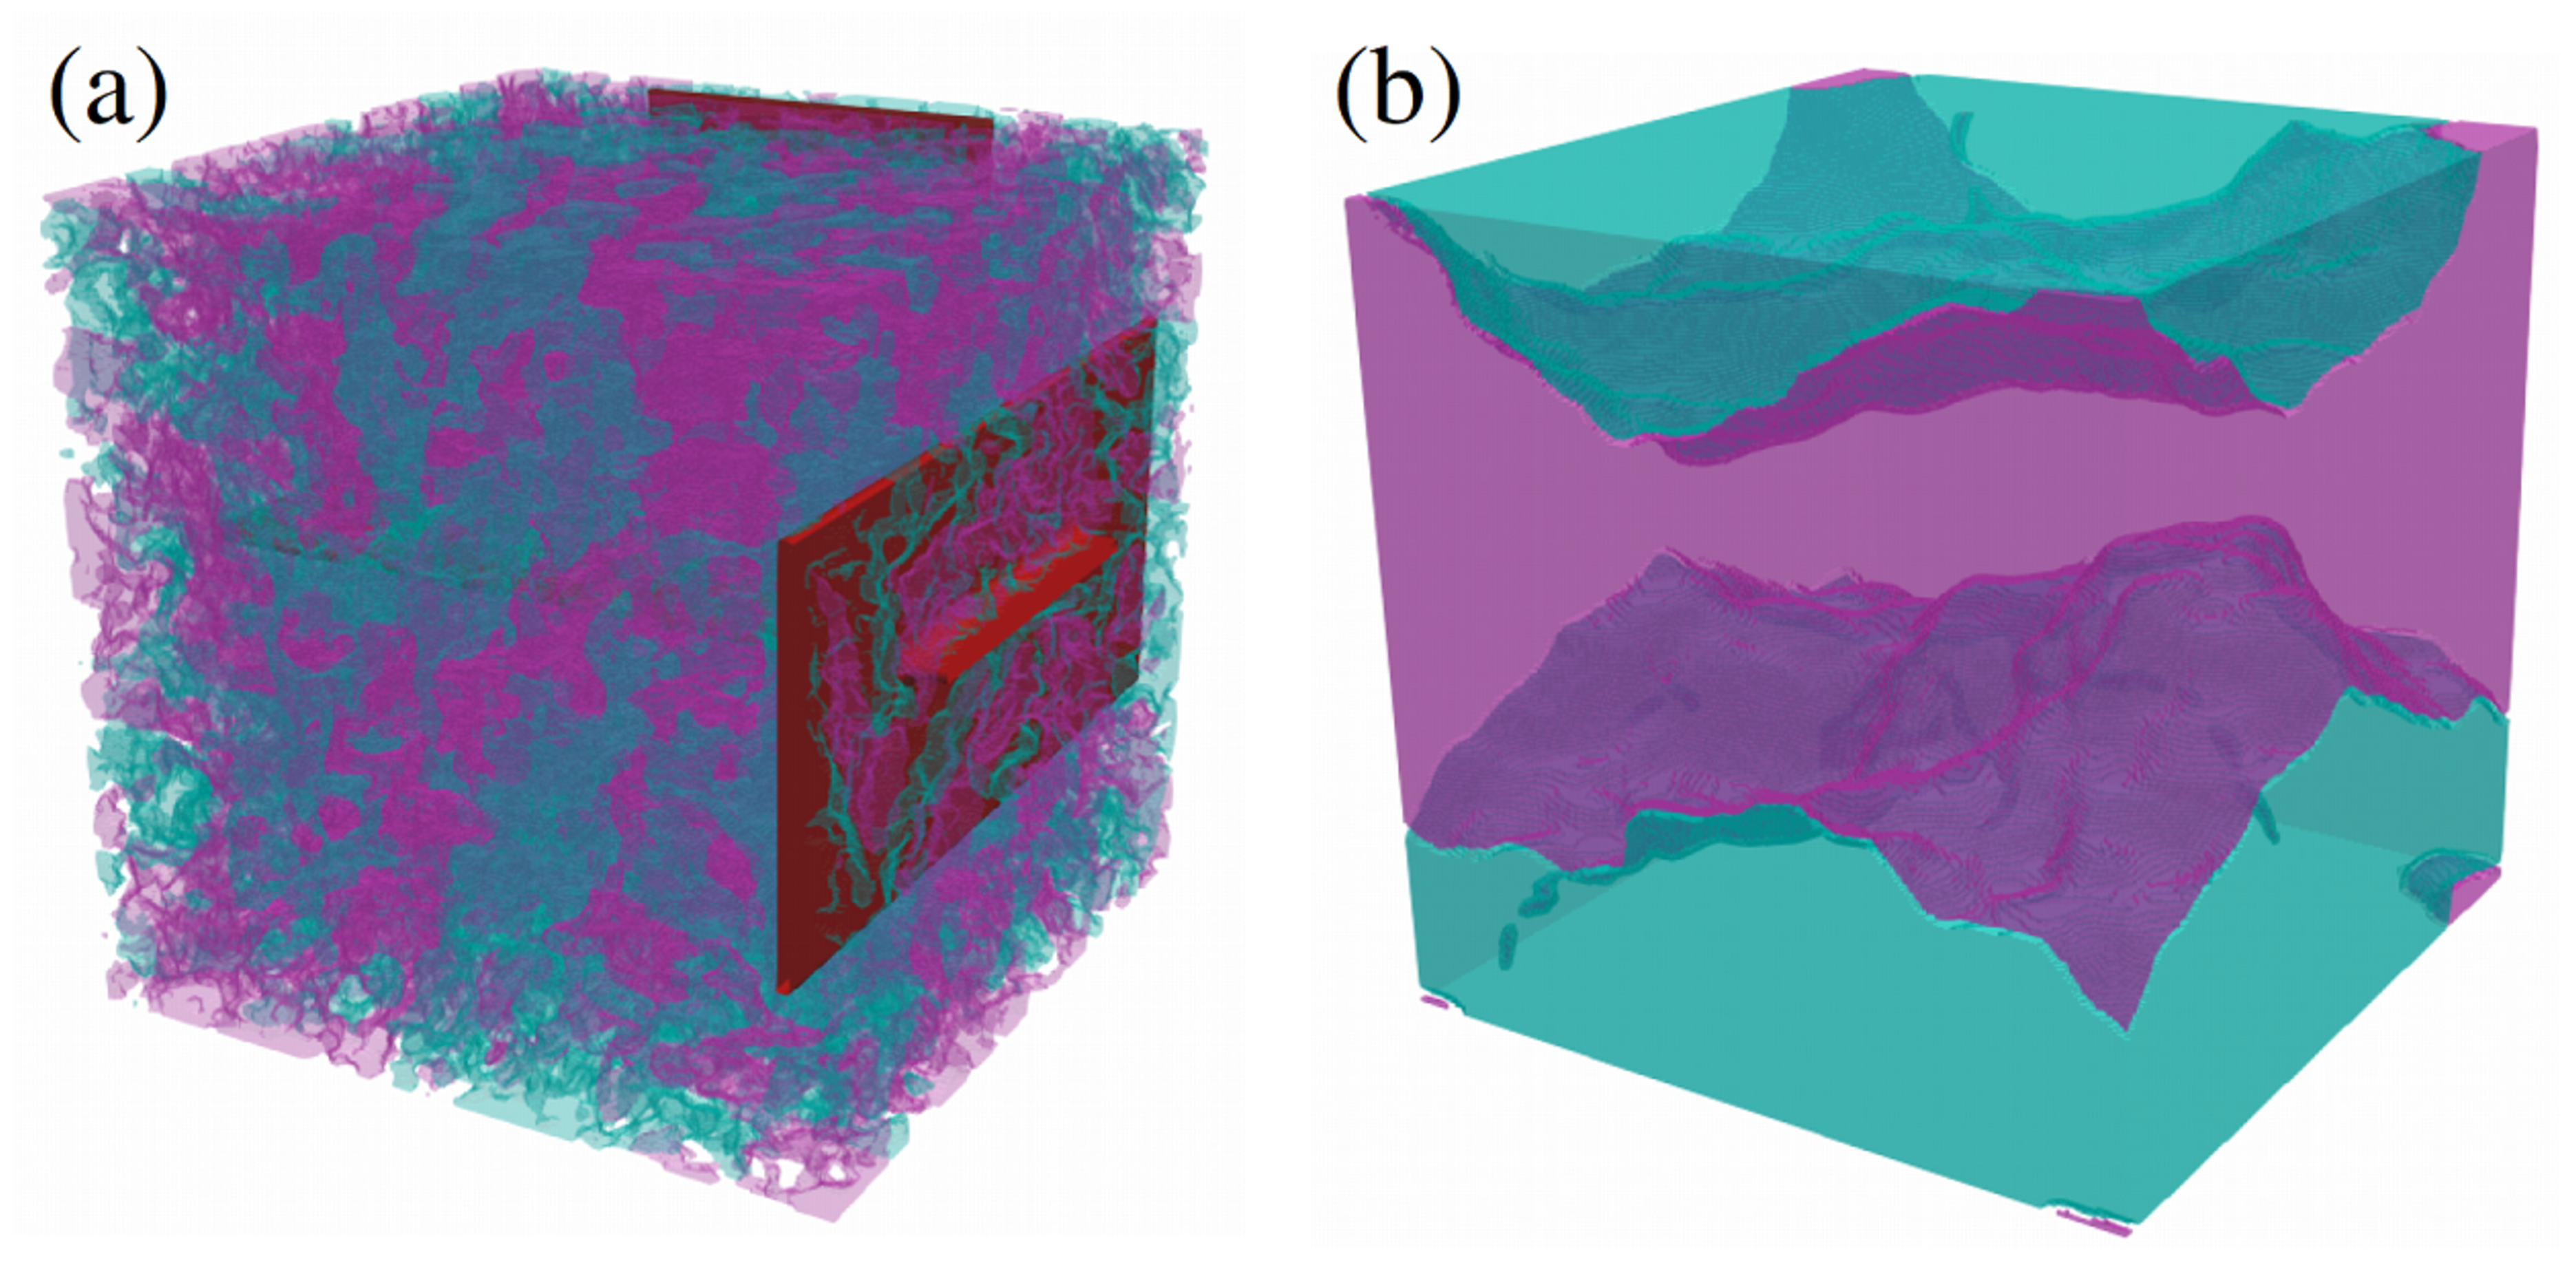
\includegraphics[width=16cm]{droplet.eps}
            \caption{
                (a)は二成分系超流動体の定常的に発達した乱流の、各成分それぞれ色分けした等密度分布を示す。
                (b)は外力によるエネルギー注入がないため、二成分が分離した状態を示す。
                二成分系の乱流では流体の界面張力と乱流による外力のバランスで、分裂するかサイズを維持するかで拮抗する。
                エネルギー注入の大小により分裂する流滴のサイズは一意に決定する。
                外力は三枚の板をそれぞれ$x,y,z$方向で往復運動させて等方性の乱流を発生させる。
                詳細は~\ref{s:twocomp}節を参照。
            }
            \label{FIG:khtop}
        \end{figure}

		\section{まえがき}
        乱流現象のメカニズムについて、一成分の系では大スケールの渦から小スケールへ繰り返し分裂するカスケードの過程が
        思い浮かぶ。一成分から二成分以上の系へ拡張すると、渦の分裂に加え、それぞれの成分ひとまとまりからの分裂が
        考えられる。成分ひとまとまりの流滴サイズは、流体の界面張力と
        乱流による外力のバランスで、分裂するかまたは現状のサイズを維持するかで拮抗する。
        本章では二成分系の超流動体を対象に、
        乱流中の流滴サイズと外力を与えるエネルギー注入率の関係について調査した内容を述べる。

		\section{古典乱流における理論的背景}
        本研究は二成分系超流動体の乱流状態における外力のエネルギー注入率と流滴サイズの関係について、
        数値計算を用いて理論的に議論した。
		一般に水と油のような互いに溶け合わない二成分系の液体に対して、
        定常的な乱流状態に発達させた場合、水滴、油滴のそれぞれの大きさは、
		与えるかき混ぜの強弱に応じて決まる。
        かき混ぜが強いと水滴と油滴のそれぞれ生成される流滴のサイズは小さく、
        かき混ぜが弱いと流滴のサイズは比較的大きくなり、
        さらに弱めてかき混ぜを止めてしまうと、水と油それぞれの範囲の二つに分離する。
        古典乱流において、コルモゴロフとヒンゼは流体が分裂する過程の
        流滴サイズについて推定した~\cite{Kolmogorov49,Hinze}。
        一般に発達した乱流では、エネルギーが大スケールの渦により注入され
        小スケールの渦の分裂とともにカスケード伝搬し、
        $-5/3$べき乗のコルモゴロフ則を示す。
        このように大スケールの渦は、周囲からの圧力の影響で
        変形、分裂などを繰り返し不安定になる。
        分裂の繰り返しで大きな流滴から小さな流滴が生成され、
        この過程は分裂させるための乱流のエネルギーと、
        流滴の形状サイズを維持するエネルギーが釣り合うまで
        続く。
        逆にこのサイズよりも小さい流滴は結合し大きな流滴に戻る。
        これらの機構により任意のエネルギー$\epsilon$の注入によって定常な乱流状態で、
        そのエネルギーに対応する一意的な流滴サイズ$D(\epsilon)$が存在する。
        以上の関係について、彼らによって~(\ref{eq:khscale})の方程式で与えられるコルモゴロフ・ヒンゼ(KH)スケールが示された。
        \begin{eqnarray}
            \label{eq:khscale}
            D \propto (\sigma/\rho)^{3/5} \epsilon^{-2/5},
        \end{eqnarray}
        $\sigma$は流滴の界面張力係数、$\rho$は周囲の流体密度、$\epsilon$は乱流中の代表的な
        エネルギー注入率を示す。
        このKHスケールは様々な実験で検証されている
        ~\cite{Clay, Shinnar, Sleicher, Arai, Deane}
        。
        またここ10年間の数値計算による研究の記録が残っている
        ~\cite{Perlekar12, Skartlien, Perlekar14, Fan, Perlekar17, Rosti}
        。

        以上の背景をもとに、二成分系BECの超流動体乱流による、
        量子力学的な系を対象に
        KHスケールについて研究を行った。
        本章では、KHスケールが超流動体の系でも現れることの他、
        量子力学的な影響によって異なるKHスケールがあることを述べる。
        超流動体における乱流の振舞いについては広く研究されている。
        単一成分の超流動で、等方的に発達した乱流状態は
        コルモゴロフ則を示すことがわかっている
        ~\cite{Nore, Stalp, Araki, Kobayashi, Parker, Baggaley}
        。
        希薄気体BECの乱流現象も実験的に研究され
        ~\cite{Henn, Neely, Kwon}
        、
        最近ではエネルギースペクトルが観測されている
        ~\cite{Thompson, Navon, Johnstone, Navon2}
        。
        理論では二次元系
        ~\cite{Nazarenko, Horng, Numasato, Bradley, Reeves}、
        ダイポール超流動体
        ~\cite{Bland}、
        境界層
        ~\cite{Stagg}.
        など様々な系で研究が行われている。
        ここでは二成分BECの乱流に焦点を当てる。
        多成分BECの乱流については多くの研究者によって調査されている
        ~\cite{Berloff, Takeuchi, Fujimoto, Tsubota, Vill, Kobyakov, Kang}
        。
        多成分BECによる領域サイズのスケーリングに関しては、
        成分の領域が形成されたあとの粗視化するダイナミクスについて広く研究されている
        ~\cite{Karl, Kudo, Hofmann, De, Nicklas, Williamson, Bourges,
        Prufer, Fujimoto18, Takeuchi18, Symes}
        。
        しかし、成分の領域サイズのスケーリングとコルモゴロフ則が組み合わさる分野の
        KHスケールについてはまだ調査されていない。

        KHスケール~(\ref{eq:khscale})とは次の機構をいう。
        乱流中の流体では、流滴サイズ$D$の領域にわたり圧力の変動を受けて
        その領域の変形、分裂を引き起こす。
        $D$の領域に対する圧力差は$\sim \rho v^2 \equiv P_{\rm turbulence}$であらわされる。
        ここで$v$は$D$の周囲に圧力を生じさせるための流体の速度差である。
        一様な等方乱流の慣性領域において、
        $v^2$の統計的な平均はコルモゴロフの$2/3$則の
        $\bar{v^2} \propto (\epsilon D)^{2/3}$に従う~\cite{Frisch}。
        よって圧力は、
        $P_{\rm turbulence} \sim \rho (\epsilon D)^{2/3}$
        であらわされる。
        一方、流滴はその形状を維持しようと分裂に対して抵抗する傾向をもつ。
        この維持する力は界面張力から生じ、形状を分裂させるための圧力は
        $\sim \sigma /D \equiv P_{\rm sustain}$と推定される~\cite{Landau}。
        さらに、KHスケール~(\ref{eq:khscale})により、
        %\begin{equation} \label{pp}
            $
            P_{\rm sustain} \sim P_{\rm turbulence},
            $
        %\end{equation}  
        の条件が満たされると、小さな流滴サイズへの分裂が止まる。
        混じり合わない二成分BECの場合、原子間相互作用と
        量子圧力から生じる界面張力は、古典流体と同様に定義されている
        ~\cite{Ao, Barankov, Schae}。
        したがって、界面$W$の厚さが流滴サイズ$D$よりもはるかに小さい場合、
        古典乱流で示される~(\ref{eq:khscale})は、超流動体の二成分BECでも現れると予想される。
        ただし$W$が$D$よりも同等か大きい場合、~(\ref{eq:khscale})の界面張力の拮抗が
        破られる。
        界面の厚さ$W$は、量子圧力と斥力相互作用の競合によって
        決まり、量子圧力が支配的になると$W$が大きくなる。
        したがって大きな$W$の限界には、分裂に対する流滴サイズを
        維持するはたらきは古典流体の$P_{\rm sustain} \sim \sigma /D$ではなく、
        量子圧力$P_{\rm sustain} \sim \hbar^2 / (m D^2)$に起因する。
        $m$は原子質量を示す。
        この場合、$P_{\rm sustain} \sim P_{\rm turbulence},$が与える流滴サイズは、
        \begin{equation} \label{qHinze}
            D \sim (\hbar / m)^{3/4} \epsilon^{-1/4}.
        \end{equation}
        であらわされる。
        したがって、$W$が大きな限界の分裂しにくい状況では、
        量子力学的な効果が顕著になり、KHスケールは$\epsilon$の$-2/5$べき乗から、$-1/4$のべき乗に
        変化すると予想される。
        本研究では
		二成分を結合するグロス・ピタエフスキー(GP)方程式の
        数値計算を用いて調査を行い、これらの予想を裏付ける。


		\section{方法}
        \label{s:twocomp}
		平均場近似において二成分BECを記述するGP方程式は、
        \begin{subequations}
        \label{eq:BIN}
        \begin{eqnarray}
			(i - \gamma)\hbar \frac{\partial \psi_1}{\partial t} & = & 
			\biggl(
				-\frac{\hbar^2}{2m}\nabla^2 + V_{\textrm{ext}}
			%\nonumber \\
			%& &
				+ g_{11}|\psi_1|^2 + g_{12}|\psi_2|^2 - \mu_1
			 \biggr) \psi_1,
			\\
			(i - \gamma)\hbar \frac{\partial \psi_2}{\partial t} & = & 
			\biggl(
				-\frac{\hbar^2}{2m}\nabla^2 + V_{\textrm{ext}}
			%\nonumber \\
			%& &
				+ g_{22}|\psi_2|^2 + g_{12}|\psi_1|^2 - \mu_2
			\biggr)\psi_2,
        \end{eqnarray}
        \end{subequations}
        であらわされる。
        $\psi_j(\bm{r}, t)$は$j$成分の波動関数である。
        $V_{\rm ext}(\bm{r}, t)$は乱流をかき混ぜて発生させる外部ポテンシャル、
        $g_{jj'} = 4 \pi \hbar^2 a_{jj'} / m$は結合定数である。
        $a_{jj'}$は$j$と$j'$の成分間の$s$波散乱長である。
        ~(\ref{eq:BIN})の定数$\gamma$は凝縮体から、
        原子が熱的にエネルギー散逸するために導入した~\cite{Choi}。
        その$\gamma$の値は、回復長よりも小さなスケールでエネルギー散逸が起きるように、
        慣性領域に影響が及ばない数値を選んだ。
        また化学ポテンシャル$\mu_j$の導入により、$\int |\psi_j|^2 d\bm{r}$が保存し、
        ユニタリー性が常に保たれる。
        数値計算は擬スペクトル法を用いて算出した。
        詳細については~\ref{s:numeric}(A)にて示す。
        二成分の混ざり具合は、結合定数$g_{jj'}$で決められる。
        $g_{12}^2 > g_{11} g_{22}$の条件の場合、二成分は混ざり合わず相分離が起きる
        ~\cite{Pethick}。
        本研究では、
        $g_{11} = g_{22} \equiv g > 0$かつ$g_{12} > 0$の状況を想定した。
        したがって、混ざり合わない条件は、
        \begin{equation} \label{im}
            g_{12} > g,
        \end{equation}
        で与えられる。
        これらの混ざり合わず相分離する条件で、成分間に界面が生成される。
        その結果、界面では界面張力によるエネルギーが生じる。
        $g_{12} / g - 1 \ll 1$の場合、界面張力の係数は、
        \begin{equation} \label{sigma}
            \sigma \simeq \left[ \frac{\hbar^2 n^3}{2m} (g_{12} - g) \right]^{1/2},
        \end{equation}
        で示される
        ~\cite{Ao, Barankov, Schae}
        。
        $n$は界面から離れた超流動体の数密度を示す。


        二成分間の界面の厚さを示す$W$は、以下の~(\ref{W})の関係で数密度が互いに$0$から$n$($n$から$0$)に変化する。
        \begin{equation} \label{W}
            W \simeq \xi (g_{12} / g - 1)^{-1/2},
        \end{equation}
        $\xi = \hbar / (2mgn)^{1/2}$は回復長を示す。


        本研究では、長さ、時間、波動関数についてそれぞれ$\xi$、$\hbar / (gn)$、$\sqrt{n}$で規格化してある。
        $n$は各成分の平均密度である。
        これらの単位系で規格化したGP方程式の結合定数は、$g_{12} / g \equiv g'$である。
        対象の系は$L^3=128^3$のサイズで周期的境界条件を課してあり、
        二成分は
        $\int |\psi_1|^2 d\bm{r} =\int |\psi_2|^2 d\bm{r} = L^3$
        の条件で占有する。
        乱流状態は、高さが$4$
        形状が$1 \times 128 \times 256$の
        板状のポテンシャル$V_{\textrm{ext}}$で流体をかき混ぜ、発生させる。
        かき混ぜ方法は図.~\ref{FIG:setup}(a)で示すように、
        周期$\nu_{\rm plate}$で、系のサイズ($0 < x < L$)を
        往復運動し大きなスケールでエネルギー注入する。
        二成分系のGP方程式~(\ref{eq:BIN})は、擬スペクトル法で数値計算を行う~\cite{Recipe}。
        詳細については~\ref{s:numeric}(A)にて示す。
        分解能はそれぞれ時間が$10^{-3}$、空間は$256^3$で、ランダムな位相を含む
        一様な密度の初期状態から時間発展させる。


		\begin{figure}[H]
			\begin{center}
			\includegraphics[width=12cm]{fig21.eps}
			\caption{
				$y$方向の幅$64$の板状ポテンシャル(赤色)が$x$軸上を等速度で往復し、定常的な乱流状態
				を発生させる。(a),(b)はそれぞれ$t=2000 \tau$のときの片方の成分$|\psi_1|^2$と
				二成分$|\psi_1|^2+|\psi_2|^2$の$z=64$の$x-y$断面を示す。板状ポテンシャルが右方向に移動し、
				$(a)$では片方の成分が$D_{\textrm{max}}=10 \sim 20$程度の大きさに分裂している。
				$(b)$では板状ポテンシャル後方から比較的大きい渦が生成されている。
				$(c)$は$-5/3$のコルモゴロフ則を満たすことを確認。
				また、散逸パラメータ$\gamma=1.0001, 1.0002, 1.0003$の条件で低波数領域に散逸エネルギーが影響していないことを確認。
				$(d)$は、$\langle v^2 \rangle = \left( \epsilon D \right)^{2/3}$で乱流状態を確認。
				$(e)$は図.~\ref{FIG:spinodal}の時間発展の様子を示す。
				$(f)$は時刻$\tau=2000$の流滴サイズの発生頻度を示す。
			}
			\label{FIG:setup}
			\end{center}
        \end{figure}
        本研究では二成分BECをかき混ぜて発達した定常乱流を取り扱う。
        図.~\ref{FIG:setup}(a)は結合定数$g'=1.5$で、板の往復するサイクルが$\nu_{\rm plate}=0.0050$の
        ときの$|\psi_1|^2$と$|\psi_2|^2$の等密度面を示す。
        $g'$が混ざり合わない条件~(\ref{im})を満たすため、二成分はそれぞれ分離した様子になる。
        また図.~\ref{FIG:setup}(a)からは、~(\ref{W})の界面厚は$W \simeq (1.5 - 1)^{-1/2} \simeq 1.4$の条件における
        代表的な流滴サイズ$D \gtrsim 10$の場合の乱流状態で$W < D$である。
        したがってこの場合のKHスケールは、(量子流体の領域の~(\ref{qHinze})ではなく)
        ~(\ref{eq:khscale})の古典流体の領域の界面厚であると期待される。詳細については後述する。
        図.~\ref{FIG:setup}(b)と(c)は、かき混ぜる板が右方向に向かっているときの、
        それぞれ密度の$|\psi_1|^2$と$|\psi_1|^2 + |\psi_2|^2$の断面を示す。
        一成分だけの図.~\ref{FIG:setup}(b)では、$|\psi_1|^2$(または$|\psi_2|^2$)が分離による
        大きな空間が見られるが、二成分の図.~\ref{FIG:setup}(c)ではかき混ぜる板の
        遠くでは一様に分布している。
        図.~\ref{FIG:setup}(c)で見える小さな密度の穴は、ポテンシャルの板の後方の
        ほぼ音速付近によって現れた量子渦である。
        コルモゴロフ則を満たした乱流の系であるかを確認するために、
        図.~\ref{FIG:setup}(d)で示すエネルギースペクトル$E(k)$を算出した。
        エネルギー散逸の係数をそれぞれ$\gamma=0.0001, 0.0002, 0.0003$で、
        非圧縮速度場の$t=1500-5000$の平均をとったものである~\cite{Nore}。
        波数空間の慣性領域($k \lesssim 0.2$)で$-5/3$べき乗のコルモゴロフ則に一致している。
        図.~\ref{FIG:setup}(d)が示す慣性領域の範囲では散逸$\gamma$による依存がほぼないことが確認できる。
        これは、$\gamma$の値によるエネルギー散逸が、慣性領域に影響を与えず小さい流滴サイズのスケールで発生していることを示している。
        本研究では散逸定数を$\gamma=0.0001$で数値計算を行った。
        %エネルギー散逸が大きいほど、小さいサイズの流滴にまで分裂しにくくなり、 % xxx
        %その結果エネルギー注入率$\epsilon$が大きい範囲でKHスケールを示さなくなる。
        KHスケールに対するエネルギー散逸の依存性については引き続き調査中である。
		\begin{figure}[H]
			\begin{center}
			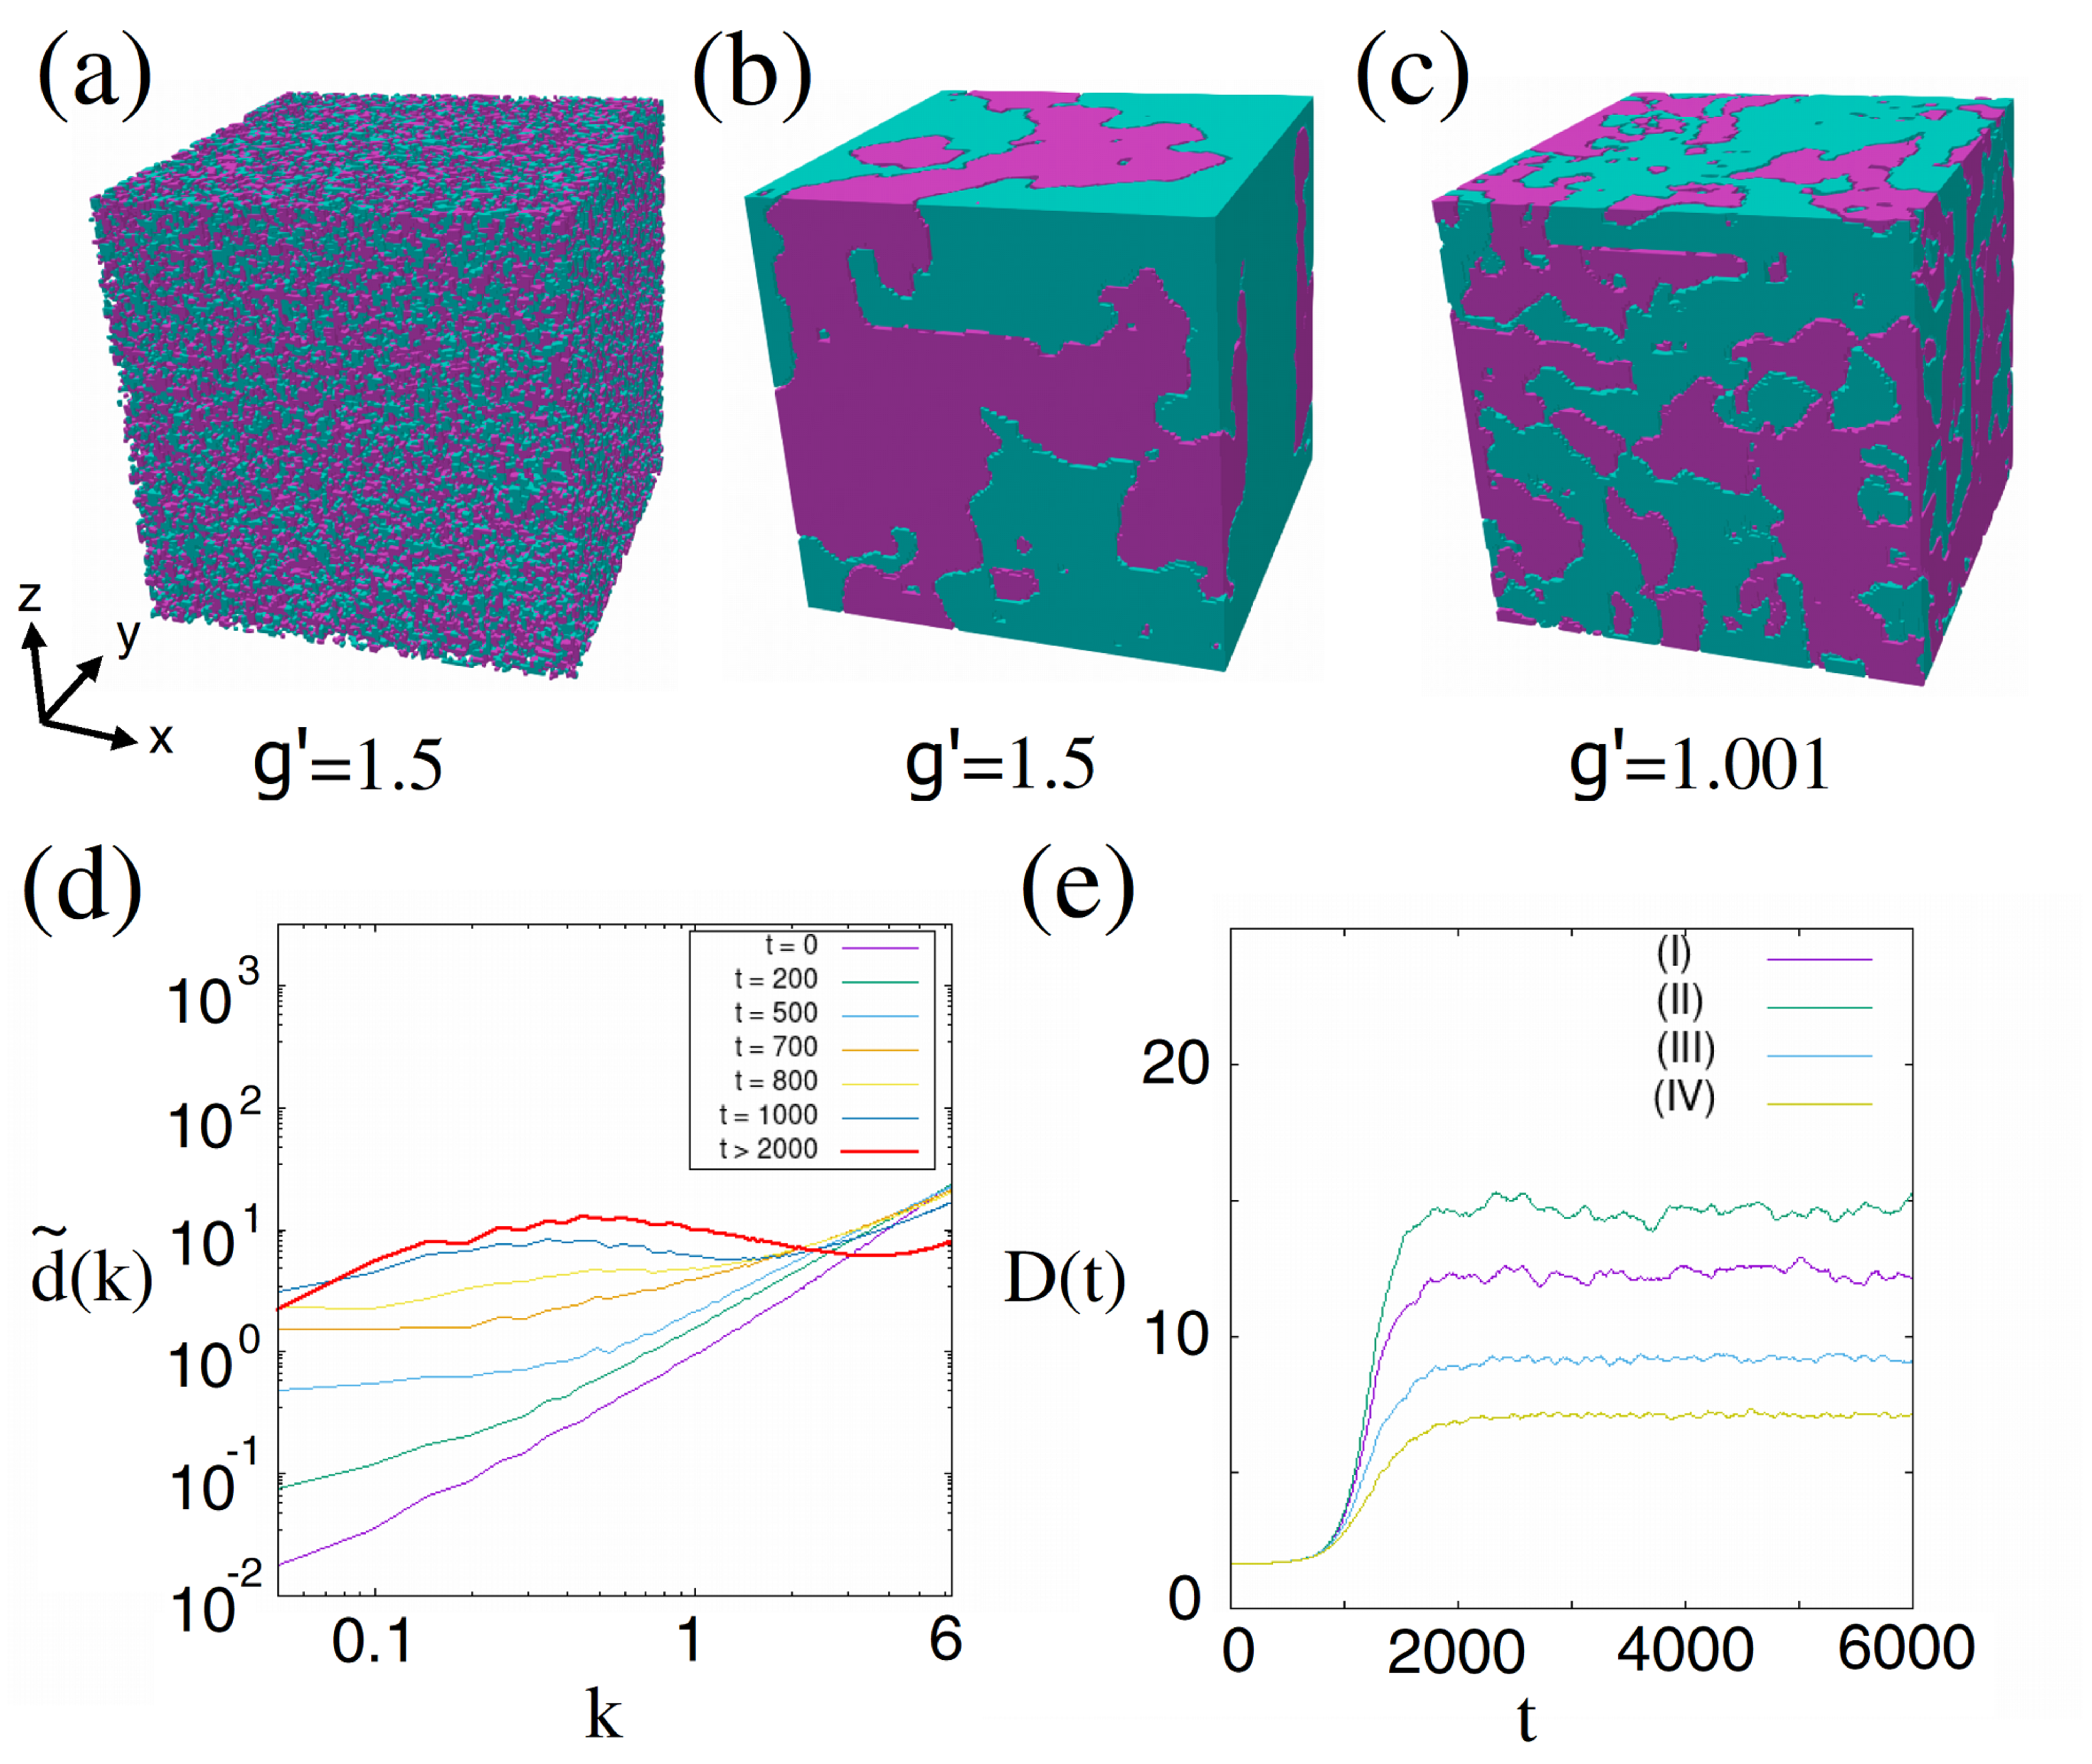
\includegraphics[width=14cm]{fig22.eps}
			\caption{
				(a)は時刻$t=1$、結合定数$g' \equiv g_{12} / g=1.5$の密度分布を示す。
                おなじく(b)は$t=5000$、$g' = 1.5$、(c)は$t=5000$、$g'=1.001$の密度分布を示す。
                (d)は$g'=1.5$、$\nu_{\rm plate}=0.01$の場合の波数空間中の頻度分布$\tilde d(k)$の時間発展を示す。
                代表的な流滴サイズはピーク値から前後$10^1$の幅のブロードな分布を示す。
                (e)は(I), (II), (III), (IV)の各条件
                ($g', \nu_{\rm plate}) = (1.001,0.006)$、$(1.5,0.005)$、$(1.5,0.008)$、$(1.5,0.01)$
                での代表的な流滴サイズが定常的になるまでの時間発展を示す。
                結合定数、注入エネルギーの大小により流滴サイズは一意に対応する。
			}
			\label{FIG:spinodal}
			\end{center}
		\end{figure}
        図.~\ref{FIG:spinodal}(a)-(c)に、$d(\bm{r})$の分布のスナップショットを示す。
        実空間$d(\bm{r})$をフーリエ変換により波数空間$\bm{k}$に展開、
        方位角の平均をとり、これを$\tilde d(k)$とあらわす。
        図.~\ref{FIG:spinodal}(d)は図.~\ref{FIG:setup}(c)の$\tilde d(k)$の時間発展をあらわす。
        ランダム位相の初期状態により、$\tilde d(k)$は$k$に対し一様な分布から始まる。
        その後、$\tilde d(k)$の分布は低波数に向かってピークが移動し、
        時刻$t \gtrsim 1500$で安定した分布に到達する。
        したがって、$\tilde d(k)$の分布は初期状態に依存しないことがわかる。

        代表的な流滴サイズ$D$は
        密度分布$\tilde d(k)$の一次積率、
        \begin{eqnarray}
            \int k \tilde d(k) dk / \int \tilde d(k) dk \equiv \langle k \rangle
        \end{eqnarray}
        から、波数の代表値を求めその平均した逆数の
        \begin{eqnarray}
            D \equiv 2\pi / \langle k \rangle
        \end{eqnarray}
        で定義する。

        %図.~\ref{FIG:spinodal}(e)は異なる条件の$g'$と$\nu_{\rm plate}$による流滴サイズ$D$の時間発展を示す。
        図.~\ref{FIG:spinodal}(e)は$g'=1.5$の場合の異なる条件の$\nu_{\rm plate}$による流滴サイズ$D$の時間発展を示す。
        この結果から、$g'$による界面張力(\ref{sigma})と、板の速度$\nu_{\rm plate}$によるエネルギー注入率で
        流滴サイズが一意的に決まることがわかる。

        %はじめに二成分の密度についてインバランスを算出する。
        %\begin{equation} \label{d}
        %    d(\bm{r}) = \left\{
        %    \begin{array}{ll}
        %        1 & (|\psi_1(\bm{r})|^2 \geq |\psi_2(\bm{r})|^2) \\
        %        -1 & (|\psi_1(\bm{r})|^2 < |\psi_2(\bm{r})|^2),
        %    \end{array} \right.
        %\end{equation}
        %これにより界面の厚さと励起による微細な粒の情報が除かれ
        %流滴サイズのみの情報を得られる。


        エネルギー注入率$\epsilon$は以下のように定義する。
        板状のポテンシャルは図.~\ref{FIG:setup}で示すように$x_{\rm plate}(t)$で
        配置され、$\pm x$方向に往復運動する。 
        ポテンシャルが運動によって超流動体から受ける力は、
        \begin{eqnarray}
            F = -\partial / (\partial x_{\rm plate}) \int
            V_{\rm ext}(\bm{r}; x_{\rm plate}) [|\psi_1(\bm{r})|^2 + |\psi_2(\bm{r})|^2]
            d\bm{r}
        \end{eqnarray}
        でもとめられる。
        したがってエネルギー注入率は
        \begin{eqnarray}
            \epsilon \equiv -F \frac{d}{dt} x_{\rm plate}
        \end{eqnarray}
        で与えられる。
        \\
        また、$\epsilon$($D$も含む)の値は、乱流のランダムな運動により
        時間変動する。
        図.~\ref{FIG:spinodal}(e)が示すように板状のポテンシャルの運動による周期的な変動が見られる。
        したがって、定常的な乱流状態の到達後の長時間にわたり平均した
        $\bar\epsilon = \langle \epsilon \rangle$と$\bar D = \langle D \rangle$の値を分析に用いる。
        図.~\ref{FIG:hinze}(a)は、$g'=1.5$と$1.001$のときの
        板の速度$\nu_{\rm plate}$に応じたエネルギー注入率の時間平均$\bar\epsilon$を示す。
		\begin{figure}[H]
			\begin{center}
			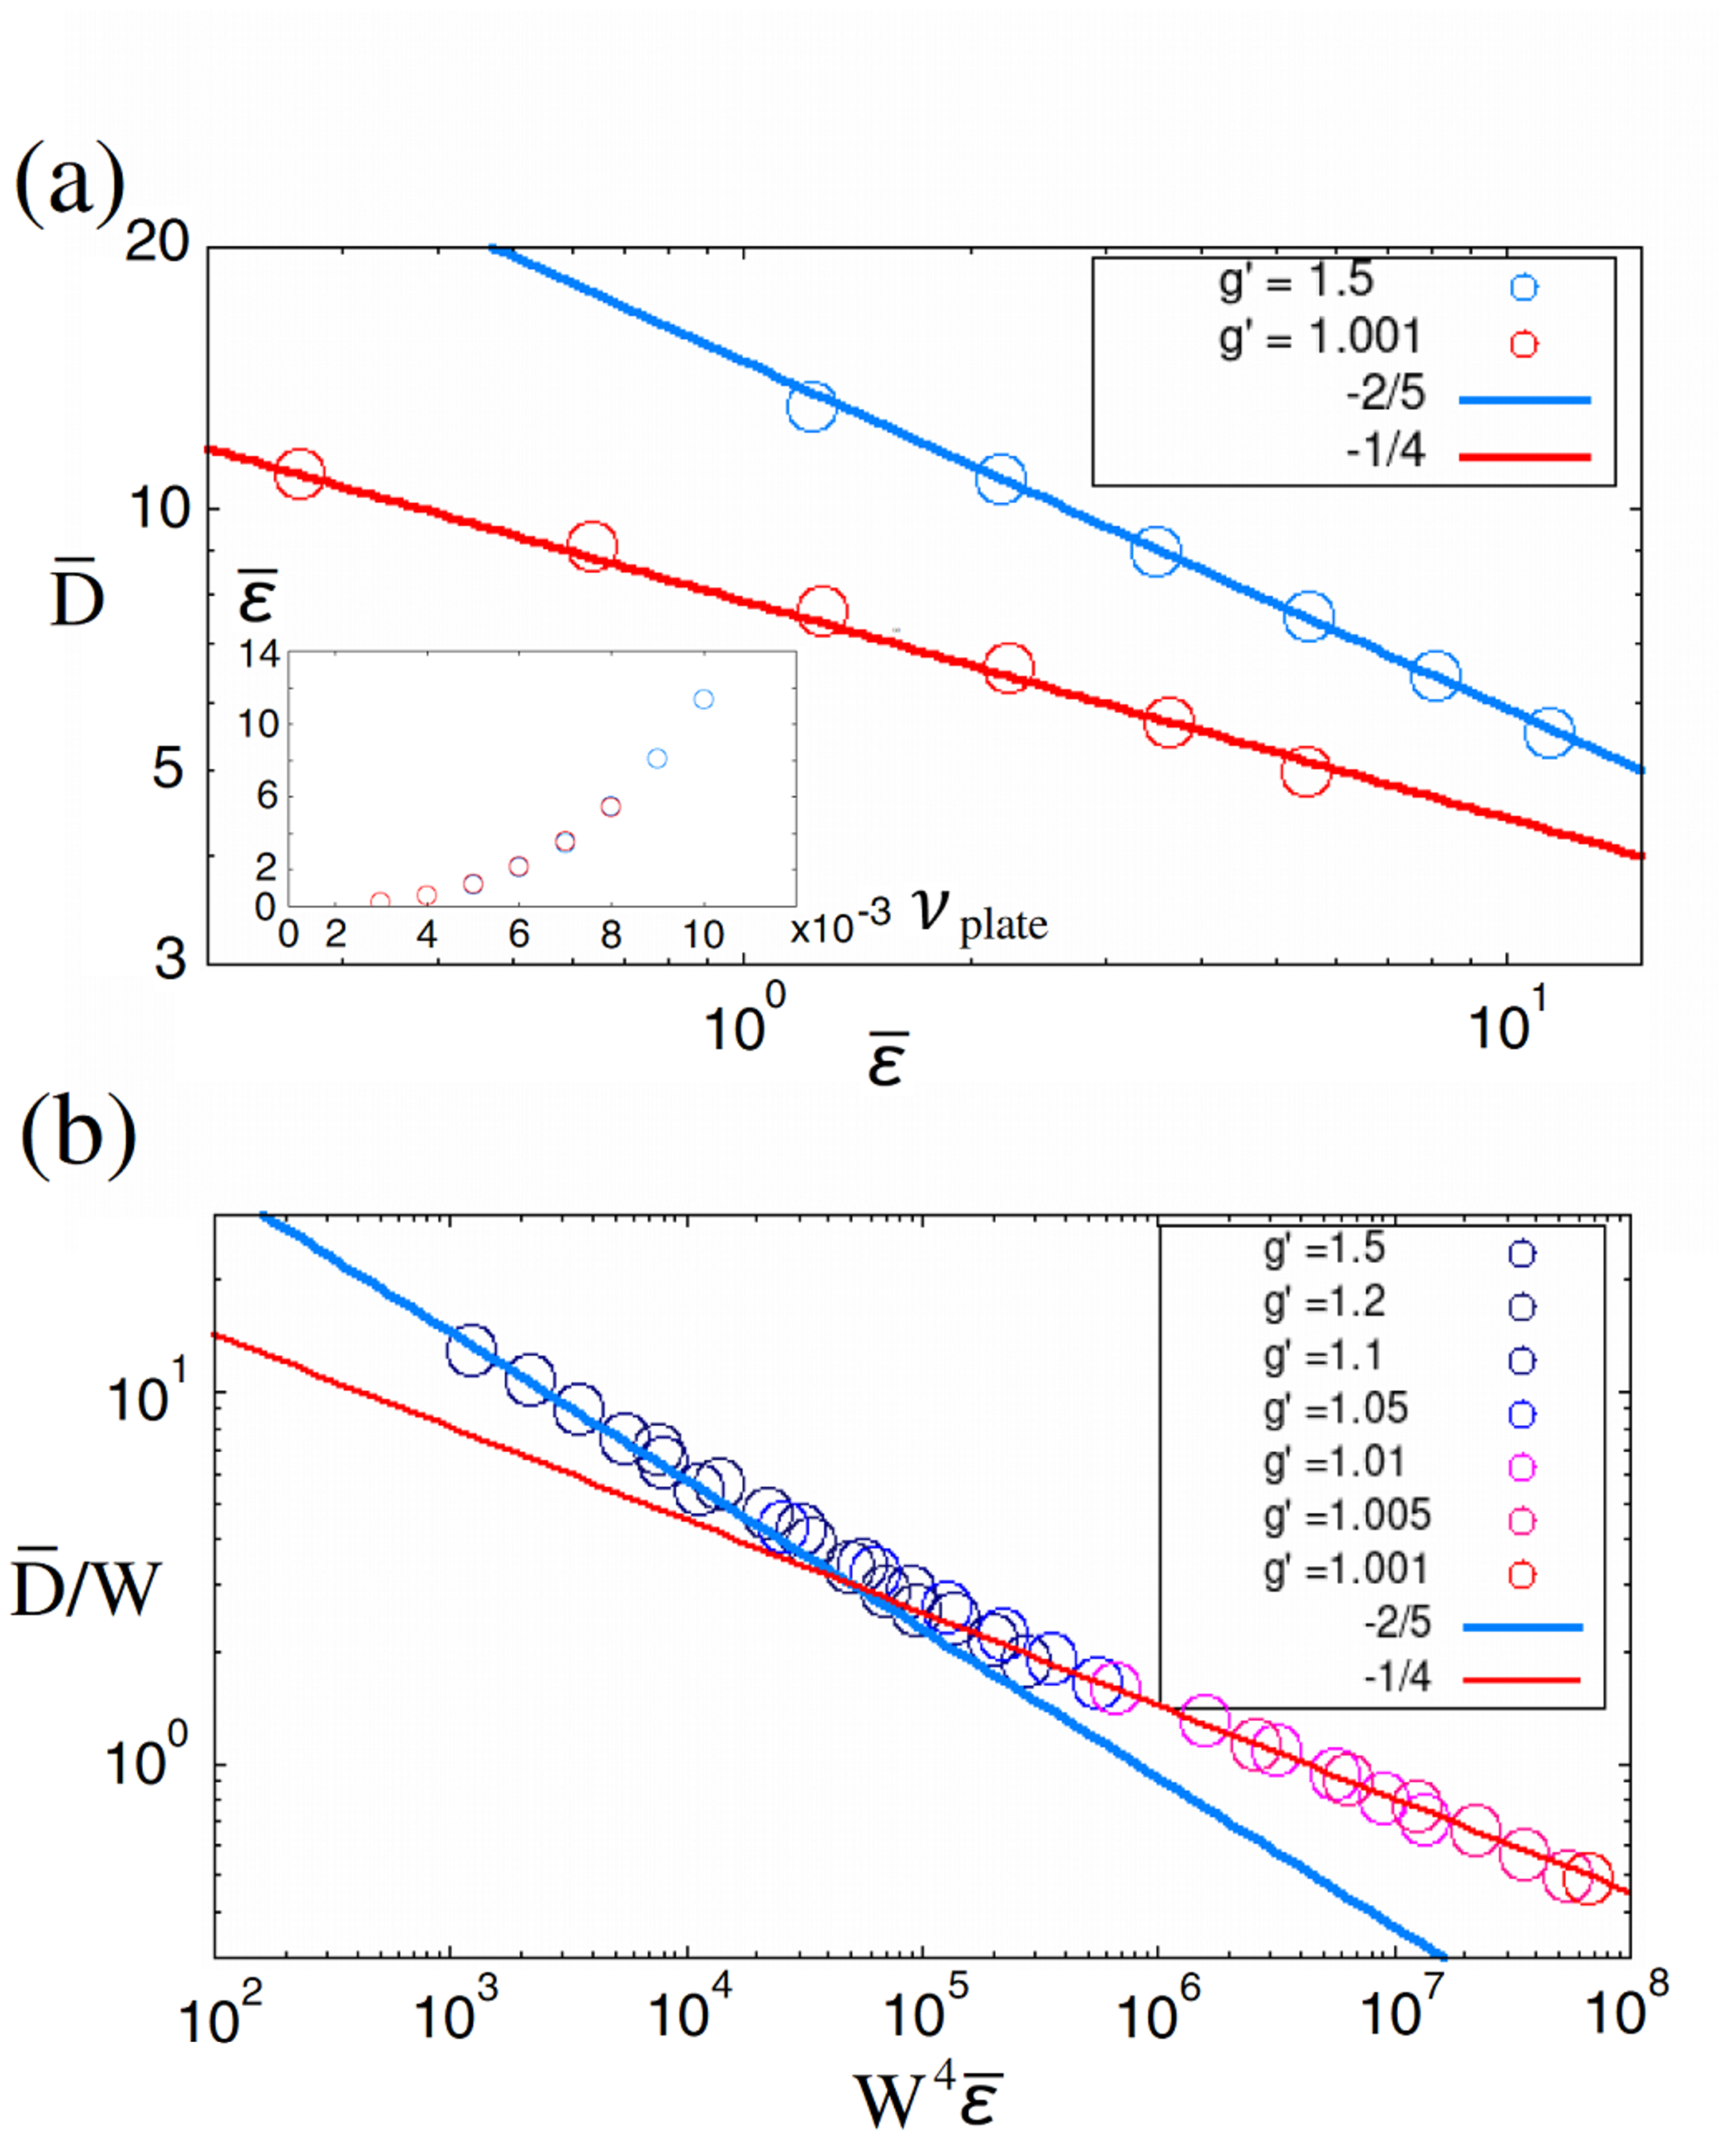
\includegraphics[width=13cm]{fig23.eps}
			\caption{
                (a)は定常的な乱流状態における$g' = g_{12}/g=1.5$と$g'=1.001$の代表的な流滴サイズ$D$と
                エネルギー注入率$\bar\epsilon$の時間平均した値をもとにプロットしたKHスケール。
                青線、赤線は~(\ref{eq:khscale})と~(\ref{qHinze})の結果と比較するための
                直線$-2/5$、$-1/4$の傾きをあらわす。
                内層のグラフは$nu_{\rm plate}$の関数としてあらわした$\bar\epsilon$を示す。
                (b)は$'g$のパラメータに対して界面厚さ$W$を用いて縮尺した$W^4 \bar\epsilon$に対する$\bar D / W$を示す。
                プロット値は縮尺された線上に揃い、普遍性をもっている。青線、赤線はそれぞれ$-2/5$、$-1/4$の傾きをあらわす。
			}
			\label{FIG:hinze}
			\end{center}
		\end{figure}
        以上の方法で、~(\ref{eq:khscale})と~(\ref{qHinze})で与えられる
        古典と量子のKHスケールについて調査する準備ができたことになる。


		\section{結果と考察}
        本研究の主題となる結果を図.~\ref{FIG:hinze}に示す。
        図.~\ref{FIG:hinze}(a)は$g'=1.5$と$1.001$の場合の、
        エネルギー注入率$\bar\epsilon$に対する代表的な流滴サイズ$\bar D$をグラフで示した。
        $g'=1.5$では、$\propto \bar\epsilon^{-2/5}$のべき乗に従い、
        ~(\ref{eq:khscale})で示す古典流体のKHスケールに一致した。
        これは二流体の成分が十分に分離されており、流滴の分裂とサイズを維持する
        メカニズムは古典流体の界面張力の範囲である。
        $g'=1.001$では、$\propto \bar\epsilon^{-1/4}$のべき乗に従い、
        ~(\ref{qHinze})で示す量子流体のKHスケールに一致した。
        これは流滴サイズを維持するメカニズムが主に不確定性原理から
        生じる量子圧力による。
        このスケールでは$\bar D < W = 0.001^{-1/2} \simeq 32$よりも
        流滴サイズが小さいために界面張力を定義することができない。
        
        ~(\ref{eq:khscale})の引用、~(\ref{qHinze})の導出と、
        図.~\ref{FIG:hinze}(a)による算出結果により、
        流滴サイズ$\bar D$と界面の厚さ$W = (g' - 1)^{-1/2}$の二つの
        大きさに応じて、異なるべき乗則が現れることがわかった。
        つぎに流滴サイズを$\bar D / W$の縮尺に代える。
        %すると~(\ref{eq:khscale})と~(\ref{qHinze})の、
        %二つのべき乗則間のクロスオーバーは$\bar D /W \sim 1$の付近にあらわれる。
        ~(\ref{qHinze})には$W$が含まれていないため、
        量子流体のKHスケールでは、
        $\bar D = c \bar\epsilon^{-1/4}$を$\bar D / W = c (W^4 \bar\epsilon)^{-1/4}$
        で置き換える。係数$c$は$W$に依存しない任意定数である。
        $\bar D / W$に対応する$W^4 \bar\epsilon$の関係は、
        $-1/4$のべき乗の範囲で普遍的にプロットされ、
        %$\bar D / W \sim 1$付近で、$-2/5$のべき乗の範囲とクロスオーバーする。
        $\bar D / W \sim 10^0$付近で、$-2/5$のべき乗の範囲とクロスオーバーする。
        そのため、このプロットは両方の範囲で普遍的であると推測される。


        図.~\ref{FIG:hinze}(b)は、広範囲をプロットするため結合定数$g'$を移動し
        $\bar D / W$に対応した$W^4 \bar\epsilon$の値である。
        広範囲で算出した結果、$-2/5$と$-1/4$のべき乗の二つの範囲は
        推測した普遍的なラインにプロットされることがわかった。
        $\bar D$と$\bar \epsilon$は数値計算上、$g'$の値ごとに狭い範囲で算出されるが、
        図.~\ref{FIG:hinze}(b)で縮尺することで$\bar D$と$\bar \epsilon$は広範囲に
        プロットされ、古典流体のKHスケールと量子流体のKHスケールの二つのべき乗則の
        存在を裏付けている。


        以上の結果について実験による再現の可能性について述べる。
        調和ポテンシャル中の非一様な二成分$|\psi_1|^2+|\psi_2|^2$から生じる
        アンバランスを回避するために、箱型のポテンシャルが推奨される。
        かき混ぜるためのポテンシャルはレーザーの共鳴光から離調させ生成する。
        光学トラップ中の攪拌を用いても乱流状態を作り出すことができる~\cite{Navon}。
        代表的な流滴サイズの計測には三次元分布の断面画像から抽出、推定が可能と考えられる~\cite{Andrews}。
        エネルギー注入率を直接測定することは難しいと思われる。
        そのため、図.~\ref{FIG:hinze}(a)のようにポテンシャルの運動とエネルギー注入率の
        関係を算出する数値計算のサポートが必要である。
        結合定数$g_{12}$についてはフェッシュバッハ共鳴法を用いて変化させることができる。
        

        %発展的な二成分系量子乱流の調査として流滴サイズ、エネルギースペクトル、スピンエネルギーの関係について分析した。
        %図.~\ref{FIG:espin}(a)の分布の
        %代表的な流滴サイズを示すピークを基点に、(b)では低波数側がコルモゴロフ則の$-5/3$のべき乗を示し、
        %(c)では高波数側でスピンエネルギーの$-7/3$のべき乗を示す~\cite{Fujimoto}。
        %得られた結果から、注入エネルギーの大小に応じて流滴サイズが一意的に決定されるほか、
        %$-5/3$べき乗の慣性領域の範囲、$-7/3$べき乗のスピンエネルギーの範囲も変化することがわかった。
        %定常の乱流において流滴サイズが一定となった状態では、
        %分裂していくまでの低波数側では乱流としてのエネルギーカスケードがはたらき、
        %高波数側では流滴サイズを維持する界面張力のエネルギーがはたらいていると推察される。
		%\begin{figure}[H]
		%	\begin{center}
		%	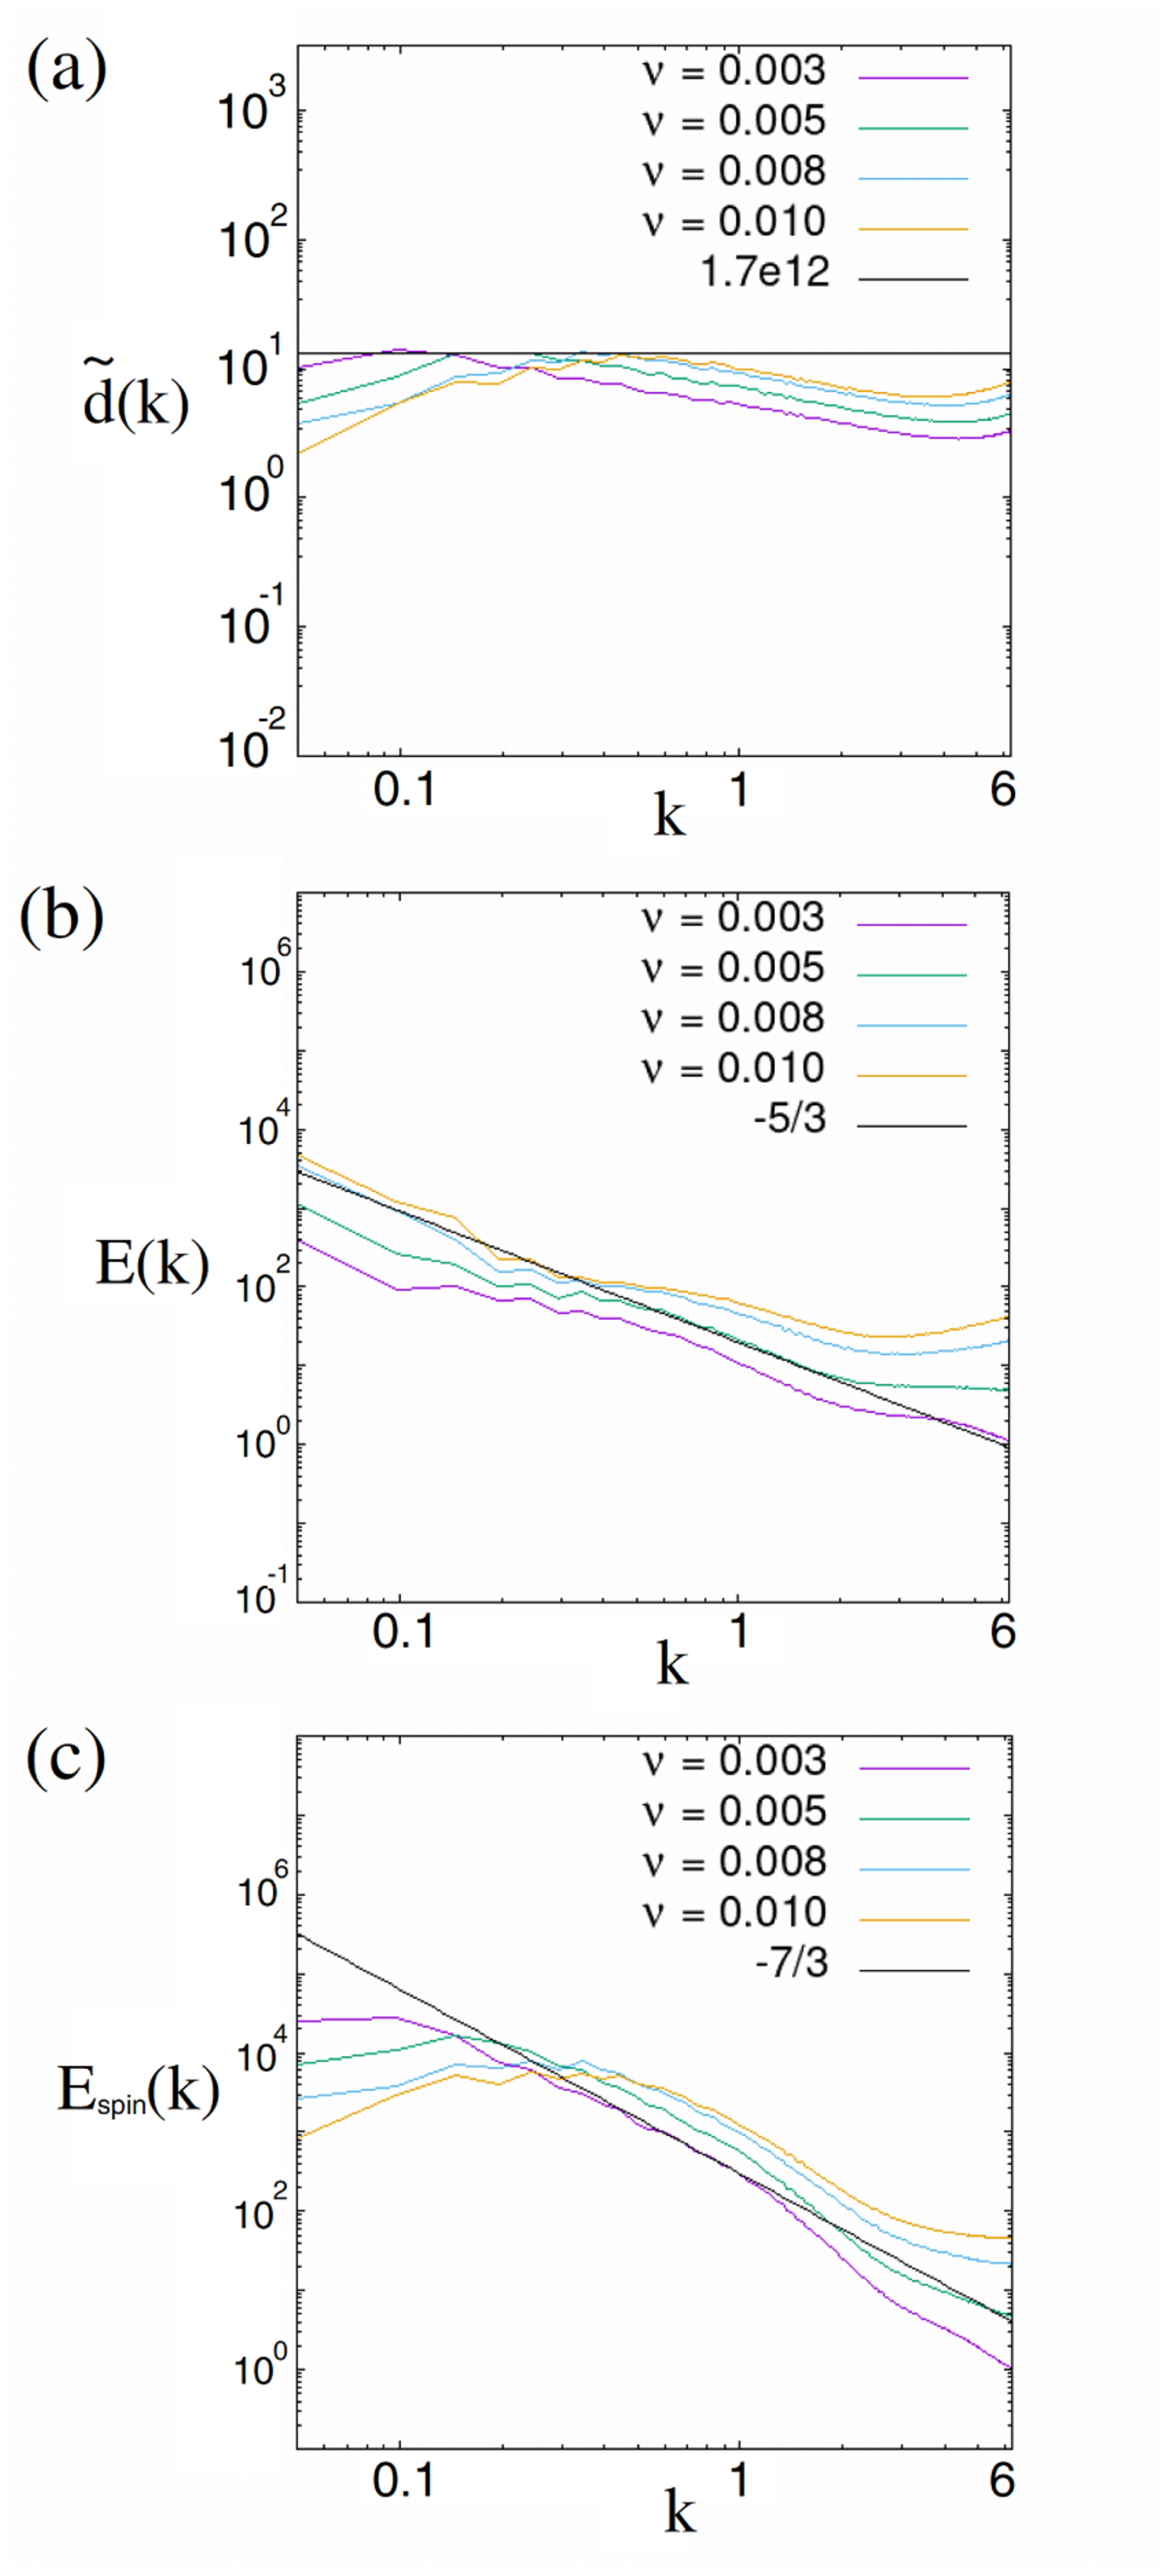
\includegraphics[width=11cm]{espin.eps}
		%	\caption{
        %        それぞれエネルギー注入率をパラメータとして$\nu=0.003, 0.005, 0.008, 0.01$で振った場合の、
        %        エネルギースペクトル、流滴サイズの分布、スピンエネルギーを示す。
		%		(a)は代表的な流滴サイズの頻度分布、
		%		(b)はエネルギースペクトル、
		%		(c)はスピンエネルギー
		%	}
		%	\label{FIG:espin}
		%	\end{center}
		%\end{figure}



		\section{むすび}
		本研究では超流動体の非圧縮二成分系の、
        発達した乱流状態におけるKHスケールについて調査分析した。
		乱流のエネルギーカスケードの慣性領域で、
		KHスケールについて古典流体と、量子力学的な不確定性が支配的となる量子流体の二種類のべき乗があることを想定した。
        二成分の超流動体を記述するGP方程式を用いて、
        外部ポテンシャルによる定常乱流を発生する数値計算を行い、
		乱流条件下で一定の注入エネルギーに$\epsilon$対して、流滴サイズ$D(\epsilon)$がKHスケールに従うことを確認した。
        さらに$D / W$と$W^4 \epsilon$の縮尺のスケーリングによって、
        量子と古典ともそれぞれ普遍的なKHスケールとなりクロスオーバーすることがわかった。
        今後の展望としては三成分以上についても拡張は可能で、同様の結論があるか引き続き研究調査を進める。


%%%%%%%%%%%% CHAPTER 5 %%%FIFTH%%%%%%%%%%%%%%%%%%%%%%%%%%%%%%%%%%%%%%%%%%%%%%%%%
	\chapter{総括}
	    本研究の
        量子乱流における渦度分布の階層構造については、
	    渦バンドルが伸張する過程で
        局所的に音速を超えた部分から量子渦が生成され、それが大スケールの渦バンドルとリコネクションを起こし、
        小スケールの渦バンドルを構成することがわかった。
	    結果として、大小の渦が直交した構造をとり高波数の方向へ漸化的に分裂しカスケードする。
        この渦度のカスケードについては古典乱流と同様であり、
	    乱流の慣性領域での$-5/3$のべき乗のエネルギースペクトルの起因を示唆している。
        古典流体、量子流体とも慣性領域での大小渦の生成する過程が
        共通であることから、
        今後の乱流研究では大規模な系などの調査によってエネルギーカスケードのメカニズムの
        より詳細な調査を進めたい。


        二成分系超流動体の乱流ではエネルギーカスケードの過程において、渦の分裂の他に二流体それぞれの分裂が伴う。
        定常乱流の系で流滴サイズとエネルギー注入率の関係性は、
		結合定数の強弱により古典乱流、量子乱流の振舞いをする
        二つのKHスケールの領域があることがわかった。
        KHスケールをもとに、
        二成分の流体は界面張力と見立てられる相互作用の効果により、乱流条件下で
		GP方程式の相互作用項が
		$g'>1.05$の領域では古典流体と同様の$-2/5$のべき乗則、
		$g'<1.05$の領域では本研究で推察した量子力学的な作用が支配する$-1/4$のべき乗則に従うことを発見した。
        この結果から、二流体の乱流で注入エネルギーに影響する流滴サイズの分析や、
        KHスケールをもとに古典的であるか量子的であるかの判別などの
        エネルギースペクトル以外の視点で分析、活用ができると考えられる。
        今後は、三流体以上の系の振る舞いについても研究を進める。


        いずれも一見複雑と思われる乱流現象に、定性的な仮説を立て定量的に分析することで
        渦バンドルのカスケード機構や、古典流体、量子流体の特性が得られ
        興味深い物理が潜んでいることがわかった。乱流分野の研究は
        物理学の未解決問題として課題が多く~\cite{Ginzburg}、
        今後も未知なるメカニズムが解明されていくと期待が持てる。
		


%%%%%%%%%%%% APPENDIX %%%%%%%%%%%%%%%%%%%%%%%%%%%%%%%%%%%%%%%%%%%%%%%%%%%%%%%%%%
	\chapter{付録}
		\appendix
		\def\thesection{付録}
        \section{(A)数値計算の方法}
            本研究の数値計算では擬スペクトル法を用いている。
            以下にグロス・ピタエフスキー方程式の数値計算の方法について示す。
            \label{s:numeric}
            三次元空間のグロス・ピタエフスキー方程式~(\ref{eq:gpe})
		    \begin{eqnarray}
                \label{eq:ngpe}
			    i \hbar \frac{\partial}{\partial t} \psi ( \Vec{r}, t ) & = &
                \left[
			    - \left( \frac{\hbar^2}{2m} \nabla^2 \right)
                + V_{\rm{ext}}(\Vec{r})
			    + g | \psi(\Vec{r}, t) |^2
                - \mu
                \right]\psi(\Vec{r},t),
		    \end{eqnarray}
            ~(\ref{eq:ngpe})の右辺の大かっこをハミルトニアン$\hat{H}$とおき、
            \begin{eqnarray}
               i \frac{\partial \psi(\Vec{r}, t)}{\partial t} =
               \hat{H} \psi(\Vec{r}, t)
            \end{eqnarray}
            とあらわす。空間と時間の初期値を$\Vec{r}_0,t_0$として波動関数は、
            \begin{eqnarray}
                \label{eq:psih}
                \psi(\Vec{r}, t) = \exp \left( -i \hat{H} t \right) \psi(\Vec{r}_0, t_0)
            \end{eqnarray}
            を得る。
            ~(\ref{eq:psih})の時刻$t$を時間発展$t+dt$に置き換え、
            \begin{eqnarray}
                \psi(\Vec{r},t+dt) & = & \exp \left[
                        -i \hat{H}(t+dt)
                    \right]
                        \psi(\Vec{r}_0,t_0)
                \\
                & = & \exp \left( -i \hat{H}dt \right) \exp \left( -i \hat{H} t \right)\psi(\Vec{r}_0,t_0) 
                = \exp \left(- \hat{H}dt \right) \psi(\Vec{r},t)
            \end{eqnarray}
            であらわせる。ハミルトニアンの運動エネルギーとそれ以外を分けると、
            \begin{eqnarray}
                \psi(\Vec{r},t+dt) & = & \exp \left[
                        -i \left \{ V_{\rm{ext}}(\Vec{r}) +g|\psi(\Vec{r},t)|^2 \right \} dt
                    \right]
                    \exp \left[
                        -i \left( -\frac{1}{2} \frac{\partial^2}{\partial \Vec{r}^2} dt \right)
                    \right] \psi(\Vec{r}, t)
            \end{eqnarray}
            を得られる。
            \\
            ここで運動エネルギーに二階の空間微分があるためフーリエ変換する。
            \begin{eqnarray}
                \exp \left[ -i \left( -\frac{1}{2} \frac{\partial^2}{\partial \Vec{r}^2} dt \right)
                    \right] \psi(\Vec{r}, t)
                & = & {\cal F}^{-1} \left[ 
                    {\cal F} \left[
                        \exp \left[
                            -i \left( -\frac{1}{2} \frac{\partial^2}{\partial \Vec{r}^2} dt \right)
                        \right]
                        \psi(\Vec{r}, t)
                    \right]
                \right]
                \\
                & = & {\cal F}^{-1} \left[
                    \exp \left[
                        -i \left( \frac{1}{2} k^2 \right) dt
                    \right]
                    \tilde{\psi}_k (t)
                \right] \ \ ( i^2 = -1 )
                \\
                & = & {\cal F}^{-1} \left[
                    \exp \left[
                        - \left( \frac{1}{2} k^2 \right) \tau
                    \right]
                    \tilde{\psi}_k (t)
                \right] \ \ (\tau \equiv i dt)
            \end{eqnarray}
            $(7)$から$(8)$へは、$\exp \left[ -i \left( -\frac{1}{2} \frac{\partial^2}{\partial \Vec{r}^2} dt\right) \right]
            \psi(\Vec{r},t) = \exp ( \tilde{A} ) \psi(\Vec{r},t)$
            とおき以下のテイラー展開を用いる。
            \begin{eqnarray}
                \exp ( \tilde{A} ) \psi(\Vec{r}, t) =
                \left[ 1 + \tilde{A} + \frac{1}{2!} \tilde{A}^2 + \cdots \right] \psi(\Vec{r},t)
            \end{eqnarray}
            と示し、フーリエ変換、
            \begin{eqnarray}
                {\cal F} \left[ \exp ( \tilde{A} ) \psi(\Vec{r},t) \right] = 
                {\cal F} \left[ \psi(\Vec{r},t) \right]
                + {\cal F} \left[ \tilde{A} \psi(\Vec{r}, t) \right]
                + {\cal F} \left[ \frac{1}{2!} \tilde{A}^2 \psi(\Vec{r},t) \right]
                + \cdots
            \end{eqnarray}
            を得る。波動関数一階の空間微分のフーリエ変換
            ${\cal F} \left[ \frac{\partial}{\partial \Vec{r}} \psi \right]=i k \tilde{\psi}_k$の関係から、
            \begin{eqnarray}
                {\cal F} \left[ \exp ( \tilde{A} ) \psi(\Vec{r},t) \right]
                & = &
                \tilde{\psi}_k (t) + \left( -i \frac{1}{2} k^2 dt \right) \tilde{\psi}_k (t)
                + \frac{1}{2!} \left( -i \frac{1}{2} k^2 dt \right)^2 \tilde{\psi}_k (t)
                + \cdots
                \\
                & = & \exp \left[ -i \left( \frac{1}{2} k^2 \right) dt \right] \tilde{\psi}_k (t)
            \end{eqnarray}
            したがって波動関数の時間発展、
            \begin{eqnarray}
                \psi (\Vec{r},t+dt) = \exp \left[
                        -i \left \{
                                V_{\rm{ext}} (\Vec{r}) + g|\psi(\Vec{r},t)|^2
                            \right \} dt
                    \right]
                    \cdot
                    {\cal F}^{-1} \left[
                        \exp \left[
                            -\left(\frac{1}{2} k^2 \right) \tau
                        \right]
                        {\cal F} \left[ \psi(\Vec{r}, t) \right]
                    \right]
            \end{eqnarray}
            を用いて三次元空間の数値計算を行う。


		\section{(B)ランダムポテンシャルの時間発展による量子乱流生成}
			\label{s:random}
			一様で等方的な量子乱流を実現するためにランダムポテンシャルを用いる。
			GP方程式のポテンシャルの項は次式であらわす。
			\begin{eqnarray}
				\label{eq:POTENTIAL}
				U( {\bm r}, t) = \sum_{\bm k} C_{{\bm k}} (t) e^{i {\bm k} \cdot {\bm r}}.
			\end{eqnarray}
			フーリエ成分$C_{\bm{k}}(t)$の時間発展はランジュバン方程式から導出される。
			\begin{eqnarray}
				\label{eq:LANGEVIN}
				\frac{{\rm d} C_{\bm k}( t)}{{\rm d}t} = -\kappa C_{\bm k}(t) + f_{\bm k}(t),
			\end{eqnarray}
            定数$\kappa > 0$はポテンシャルの時間変動を与える。
            $f_{\bm k}(t)$はガウシアン・ノイズ
			\begin{eqnarray}
				\langle f_{\bm k}(t) \rangle = 0,
			\end{eqnarray}
            で与え、その平均はゼロである。
			\begin{eqnarray}
				\langle f_{\bm k}(t) f_{{\bm k}^\prime}(t^\prime)\rangle =
				A_{\bm k}\delta_{{\bm k}{\bm k}^\prime}\delta(t-t^\prime).
			\end{eqnarray}
            の自己相関関数を得る。
			振幅 $A_{\bm k}$ は、
			\begin{eqnarray}
				\label{eq:RANDOM}
				A_{\bm k} = A_0 e^{-\left(\frac{l}{2}|\bm{k}|\right)^2},
			\end{eqnarray}
			で与えられる。
			$l$ は境界条件の範囲内でランダムポテンシャルの代表的な大きさを決める。
			ランジュバン方程式~(\ref{eq:POTENTIAL})の解を用いて、時間相関
			\begin{eqnarray}
				\langle
					C_{\bm k}(t)
					C_{{\bm k}^\prime}(t^\prime)
				\rangle
				\equiv \frac{A_{\bm k}}{2 \kappa} \delta_{{\bm k}{\bm k}^\prime} e^{-\kappa|t-t^\prime|},
			\end{eqnarray}
            が定義され、
            ランダムポテンシャルは、
			\begin{eqnarray}
				\langle
					U({\bm r}, t) U({\bm r}^\prime, t^\prime)
				\rangle \propto
				e^{-\kappa |t-t'|} e^{|\bm{r}-\bm{r}'|^2/l^2}.
			\end{eqnarray}
            を得る。
			~\ref{s:distributions}節の数値計算では、
            ランジュバン方程式~(\ref{eq:LANGEVIN})に従う係数$C_{\bm k}(t)$であらわせる。
            ~(\ref{eq:POTENTIAL})の逆フーリエ変換により空間$l$、時間$\kappa^{-1}$のスケールで
            実空間のランダムポテンシャルを与える。


		\section{(C)非圧縮性流体のエネルギースペクトル}
		乱流におけるエネルギーカスケードを担うのは、
        慣性領域で流体の密度が一定の非圧縮の流れである。
		\label{s:pspectrum}
		量子流体中の運動エネルギーは以下のようにあらわせる。
		\begin{eqnarray}
			E_{{\rm kinetic}} & = & -\frac{1}{2} \int {\rm d}\bm{r} \tilde{\psi}^* \tilde{\nabla}^2 \tilde{\psi},
			\\
			& = & \frac{1}{2}\int {\rm d}\bm{r}|\tilde{\nabla} \tilde{\psi}|^2.
		\end{eqnarray}
		波動関数$\tilde{\psi}(\bm{r}) = \sqrt{\rho(\bm{r})} e^{i \phi(\bm{r})}$,
		を用いて運動エネルギーの項を二つに分けられる。
		\begin{eqnarray}
			E_{{\rm kinetic}} & = & \frac{1}{2}\int {\rm d}\bm{r}\left[
			\rho(\tilde{\nabla} \phi)^2 + (\tilde{\nabla} \sqrt{\rho})^2
			\right],
			\\
			& = & E_1 + E_2,
		\end{eqnarray}
        $E_1=\frac{1}{2}\int {\rm d}\bm{r} \rho(\tilde{\nabla} \phi)^2$
		は古典流体としての運動エネルギー
		と、
        $E_2=\frac{1}{2}\int {\rm d}\bm{r} (\tilde{\nabla} \sqrt{\rho})^2$
        は量子圧力が起因するエネルギーの項である。
		実空間での渦度ベクトル$\bm{w}(\bm{r})=\sqrt{\rho(\bm{r})}\tilde{\nabla}\tilde{\phi}(\bm{r})$
        と波数空間での渦度ベクトルとしてフーリエ変換、
		\begin{eqnarray}
			\tilde{\bm{w}}(\bm{k}) \equiv \int \bm{w}(\bm{r}) e^{-i \bm{k} \cdot \bm{r}} {\rm d} \bm{r}.
		\end{eqnarray}
        を定義する。
		以下の様に、速度場$\bm{w}$を圧縮と非圧縮に分ける。
		\begin{eqnarray}
			\tilde{\bm{w}}(\bm{k}) & = &
			\frac{\bm{k}\cdot\tilde{\bm{w}}(\bm{k})}{k^2}\bm{k}
			+ \frac{(\bm{k}\times\tilde{\bm{w}})\times\bm{k}}{k^2},
			\\
			\tilde{\bm{w}}_{\rm L} & = &
			\frac{\bm{k}\cdot\tilde{\bm{w}}(\bm{k})}{k^2}\bm{k},
			\\
			\tilde{\bm{w}}_{\rm T} & = &
			\frac{(\bm{k}\times\tilde{\bm{w}})\times\bm{k}}{k^2}.
			\end{eqnarray}
			運動エネルギーを速度場の表記で書き換える。
			\begin{eqnarray}
			E_1 & = & \frac{1}{2} \int {\rm d}\bm{r}\left|\bm{w}(\bm{r})\right|^2,
			\\
			& = & \frac{1}{2}\int {\rm d}\bm{r} \left[
				\left| \bm{w}_{{\rm T}}(\bm{r})\right|^2
				+ \left| \bm{w}_{{\rm L}}(\bm{r})\right|^2
			\right].
		\end{eqnarray}
		流体の運動エネルギーの非圧縮成分のみを抽出し、
		\begin{eqnarray}
			E_1^{{\rm ic}}
			& = & \frac{1}{2} \int \left|\bm{w}_{{\rm T}}(\bm{r}) \right|^2 {\rm d}\bm{r},
			\\
			& = & \frac{1}{2}\int\frac{{\rm d}{\bm k}}{(2 \pi)^3}
			\tilde{\bm{w}}_{{\rm T}}(\bm{k}) \cdot \tilde{\bm{w}}_{{\rm T}}(-\bm{k}),
			\\
			& = & \int {\rm d}k E(k),
		\end{eqnarray}
		を、非圧縮流体に関するエネルギースペクトル$E(k)$と定義する。	


        図.~\ref{FIG:incompressible}は、超流動体における
        発達した定常乱流の非圧縮、圧縮それぞれのエネルギースペクトルの例を示す。
		\begin{figure}[H]
			\centering
			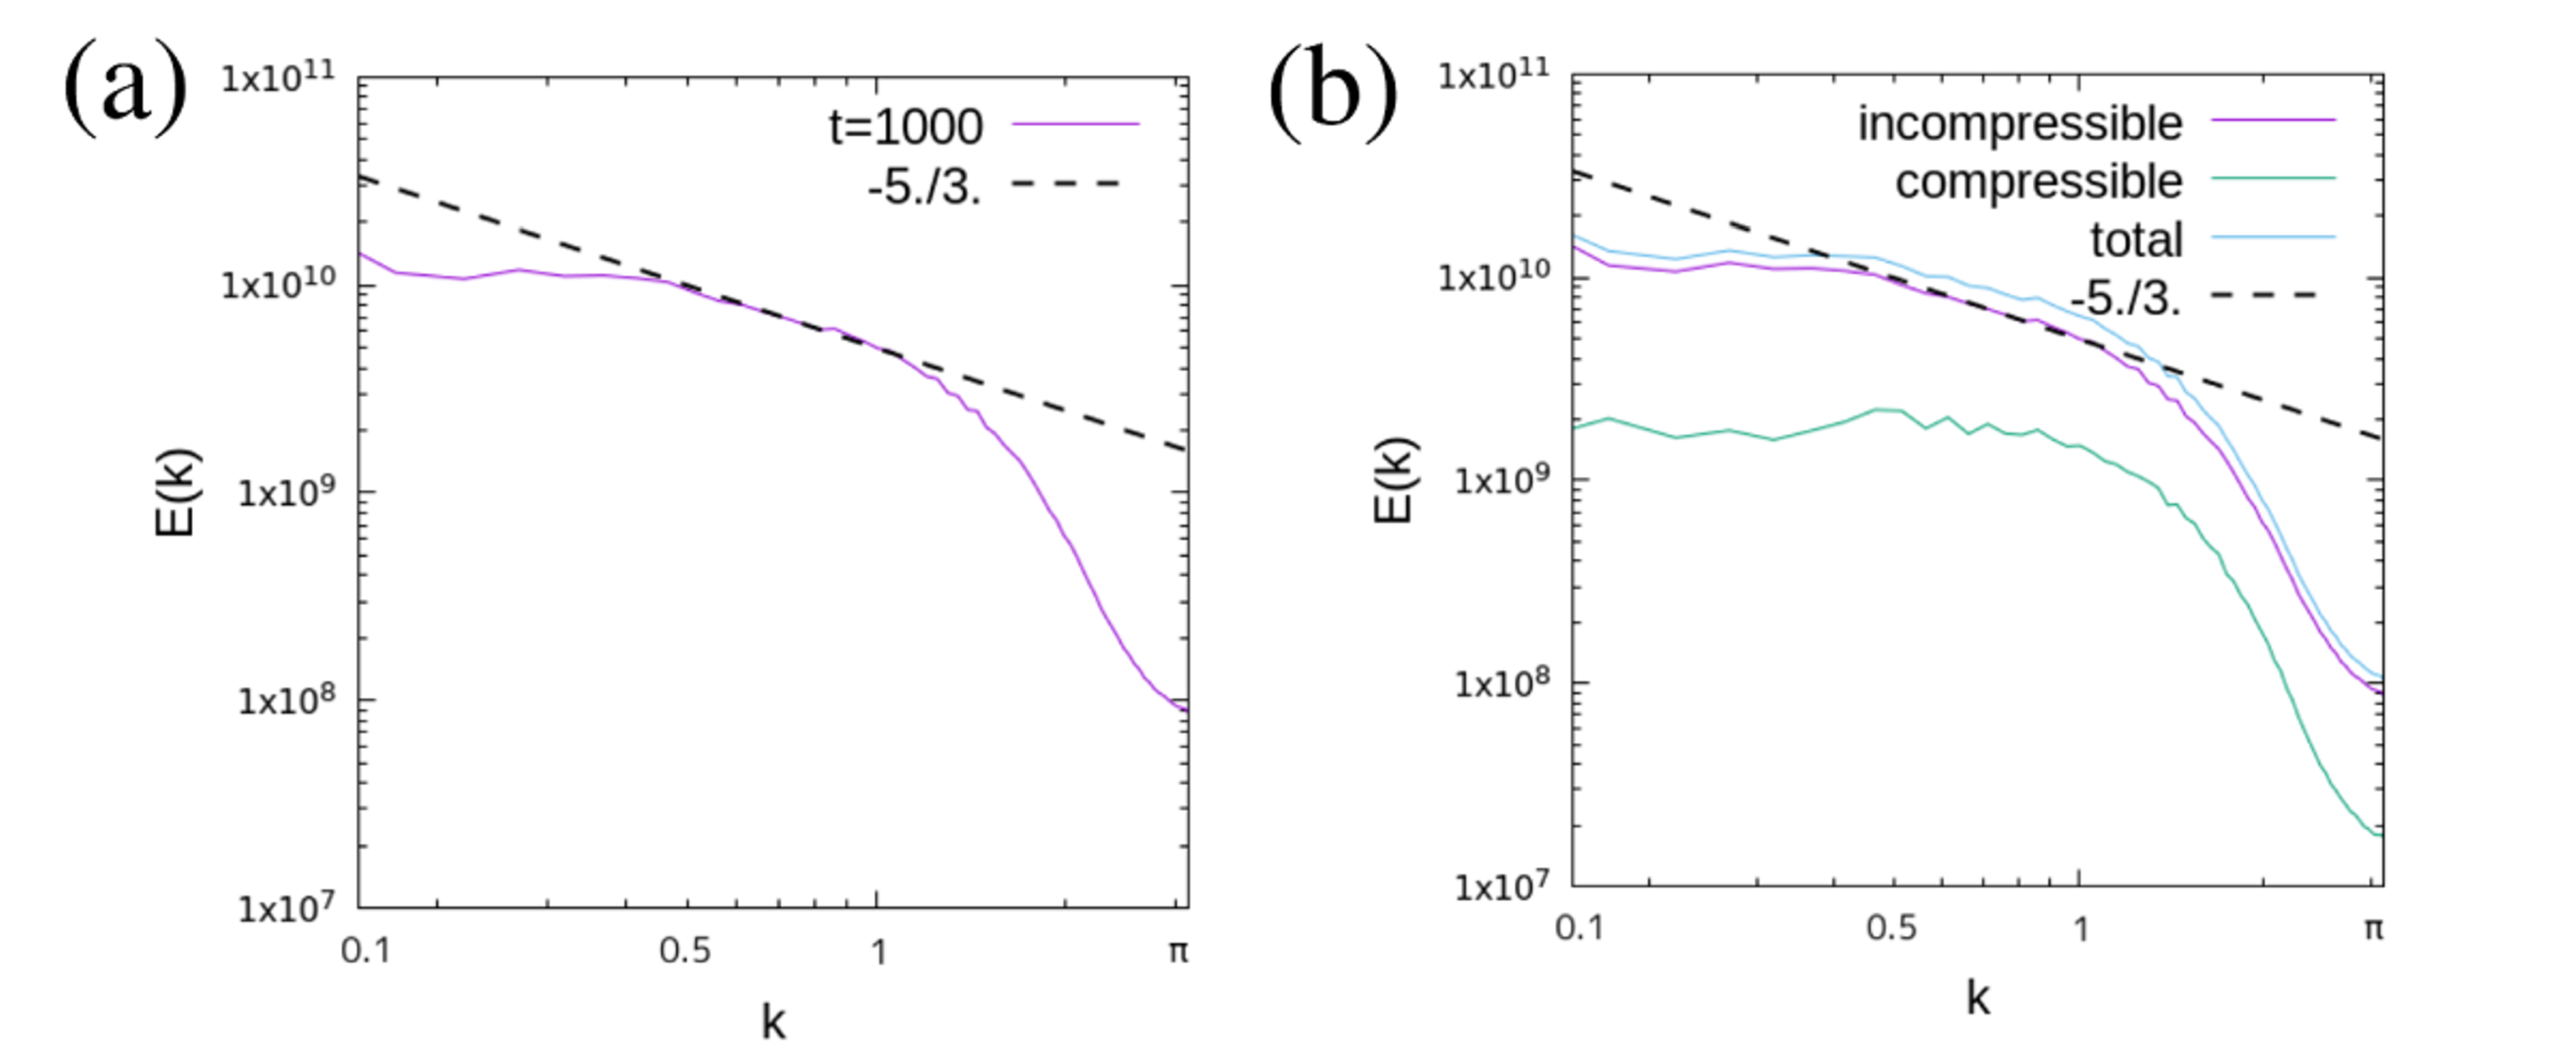
\includegraphics[width=16cm]{incompressible.eps}
			\caption{
			(a)は図.~\ref{FIG:turbulent}$(c^{\prime})$の$t=1000$の非圧縮のエネルギースペクトルを示す。
            (b)は同時刻の、紫色線が非圧縮、緑色線が圧縮、水色線がそのトータルのエネルギースペクトルを示す。
            非圧縮流れの成分のエネルギースペクトルが$-5/3$べき乗のコルモゴロフ則を示す。
			}
			\label{FIG:incompressible}
		\end{figure}


%%%%%%%%%%%% REFERENCE %%%%%%%%%%%%%%%%%%%%%%%%%%%%%%%%%%%%%%%%%%%%%%%%%%%%%%%%%
    \renewcommand{\bibname}{参考文献}
	\begin{thebibliography}{99}
%%%%%%%%%%%%%%%%%%%%%%%%%%%%%%%%%%%%%%%%%%%%%%%%%%%%%%%%%%%%%%%%%%%%%%%%%%%%%%%%
%		CHAPTER 1
%%%%%%%%%%%%%%%%%%%%%%%%%%%%%%%%%%%%%%%%%%%%%%%%%%%%%%%%%%%%%%%%%%%%%%%%%%%%%%%%
		\bibitem{Kolmogorov}
		A. N. Kolmogorov,
		The local structure of turbulence
		in incompressible viscous fluid for very large Reynolds numbers,
		Dokl. Akad. Nauk. SSSR \textbf{30}, 299 (1941).

		\bibitem{Batchelor}
		G. K. Batchelor, and I. Proudman,
		The effect of rapid distortion of a fluid in turbulent motion,
		%The Quarterly Journal of Mechanics and Applied Mathematics, \textbf{7}, 83(1954).
		Quart. J. Mech. Appl. Math. \textbf{7}, 83 (1954).

		\bibitem{Tatsumi1}
		T. Tatsumi,
		The theory of decay process of incompressible isotropic trubulence,
		%{\it Proceeding of the Royal Society of London} A , \textbf{239}, 16 (1957).
		Proc. R. Soc. London, Ser. A \textbf{239}, 16 (1957).

		\bibitem{Tatsumi2}
		巽 友正,
		乱流,
		槇書店, 15 (1962).
		
  		\bibitem{Kraichnan}
  		R. H. Kraichnan,
  		On Kolmogorov's inertial-range theories,
  		J. Fluid Mech. \textbf{62}, 305 (1974).

		\bibitem{Frisch1}
		U. Frisch, P. L. Sulem, and M. Nelkin,
		A simple dynamical model of intermittent fully developed turbulence,
		J. Fluid Mech. \textbf{87}, 719 (1978).

		\bibitem{Frisch2}
		% The Legacy of A. N. Kolmogorov
		U. Frisch, {\it Turbulence: The Legacy of A. N. Kolmogorov},
		(Cambridge University Press, Cambridge, UK, 1995).

        \bibitem{Cyril}
        C. Cichowlas, P. Bona\"iti, F. Debbasch, and M. Brachet,
        Effective Dissipation and Turbulence in Spectrally Truncated Euler Flows,
		Phys. Rev. Lett. {\bf 95}, 264502 (2005).

        \bibitem{Navon}
        N. Navon, A. L. Gaunt, R. P. Smith, and Z. Hadzibabic,
        Emergence of a turbulent cascade in a quantum gas,
        Nature (London) \textbf{539}, 72 (2016).

		\bibitem{Kobayashi1}
		M. Kobayashi, and M. Tsubota,
		Kolmogorov spectrum of superfluid turbulence:
		Numerical analysis of the Gross-Pitaevskii equation
		with a small-scale dissipation,
		Phys. Rev. Lett. \textbf{94}, 065302 (2005).

		\bibitem{Kobayashi2}
		M. Kobayashi, and M. Tsubota,
		Thermal dissipation in quantum turbulence,
		Phys. Rev. Lett. \textbf{97}, 145301 (2006).

		\bibitem{Kobayashi3}
		M. Kobayashi, and M. Tsubota,
		Quantum turbulence in a trapped Bose-Einstein condensate,
		Phys. Rev. A \textbf{76}, 045603 (2007).

        \bibitem{Araki}
        T. Araki, M. Tsubota, and S. K. Nemirovskii,
        Energy Spectrum of Superfluid Turbulence with No Normal-Fluid Component,
        Phys. Rev. Lett. \textbf{89}, 145301 (2002).

		\bibitem{paper1}
		Tsuyoshi Kadokura, and Hiroki Saito,
		Orthogonal and antiparallel vortex tubes and energy cascades in quantum turbulence,
		Phys. Rev. Fluids {\bf 3}, 104606 (2018).

        \bibitem{Ginzburg}
        Vitaly Lazarevich Ginzburg,
        {\it The Physics of a Lifetime.
        Reflections on the Problems and Personalities of 20th Century Physics}, (Berlin: Springer-Verlag, 2001).

		\bibitem{Richardson}
		L. F. Richardson,
		% Lewis Fry Richardson 1881-1953
		% Richardson number
		% "Big whirls have little that feeds on their velocity,
		%  and little whirls have lesser whirls and so on viscosity."
		% L. F. Richardson, {\it Weather Prediction by Numerical Process},
		% (Cambridge University Press, Cambridge, 1922).
		{\it Weather Prediction by Numerical Process},
		(Cambridge University Press, Cambridge, UK, 1922).

		\bibitem{Goto1}
		S. Goto,
		A physical mechanism of the energy cascade
		in homogeneous isotropic turbulence,
		J. Fluid Mech. \textbf{605}, 355 (2008).

		\bibitem{Goto2}
		S. Goto, Y. Saito, and G. Kawahara,
		Hierarchy of antiparallel vortex tubes
		in spatially periodic turbulence at high Reynolds numbers,
		Phys. Rev. Fluids \textbf{2}, 064603 (2017).

		\bibitem{Goto3}
		S. Goto,
		Coherent structures and energy cascade in homogeneous turbulence,
		% Progress of Theoretical Physics Supplement \textbf{195}, 1 July 2012, Pages 139-156.
		Prog. Theor. Phys. Suppl. \textbf{195}, 139 (2012).

        \bibitem{Kolmogorov49}
        A. N. Kolmogorov,
        On the breakage of drops in a turbulent flow,
        Dokl. Akad. Nauk. SSSR \textbf{66}, 825 (1949).

        \bibitem{Hinze}
        J. O. Hinze,
        Fundamentals of the Hydrodynamic Mechanism of Splitting in Dispersion Process,
        AIChE J. \textbf{1}, 289 (1955).

        \bibitem{Planck}
        Max Planck,
        \"{U}ber eine Verbesserung der Wienschen Spektralgleichung,
        Verhandlungen der Deutschen Physikalischen Gesellschaft {\bf 2} (1900).

		\bibitem{A.Einstein1}
		A. Einstein,
		\"{U}ber einen die Erzeugung und Verwandlung des Lichtes betreffenden heuristischen Gesichtspunkt,
		Ann. Physik {\bf 17}, 132 (1905).

		\bibitem{Wien}
		W. Wien,
		Uber die Energievertheilung im Emissionsspectrum eines schwarzen K\"{o}rpers,
		Ann. Physik {\bf 294}, 662 (1896).

		\bibitem{Rayleigh}
		L. Rayleigh,
		Remarks upon the law of Complete Radiation,
		Phil. Mag. {\bf 49}, 539 (1900).

		\bibitem{S.N.Bose}
		S. N. Bose, 
		Planck's law and the light quantum hypothesis,
		Z. f\"{u}r Phys. {\bf 26}, 178 (1924).

		\bibitem{A.Einstein2}
		A. Einstein,
		Quantentheorie des einatomigen idealen Gases,
		%Sitzungsberg K.Preuss. Akad. Wiss.,
		%Phys. Math. {\bf K1}. No.22, 261(1924); No. 1,3(1925).
		Sitz. Ber. Kgl. Preuss. Akad. Wiss. {\bf 22} 261 (1924);
		Sitz. Ber. Kgl. Preuss. Akad. Wiss. {\bf 23} 3 (1925).

		\bibitem{Anderson}
		Anderson M. H., J.R. Ensher, M.R.Matthews, C.E.Wieman, and E.A.Cornell,
		Observation of Bose-Einstein Condensation in a Dilute Atomic Vapor,
		Science {\bf 269}, 198 (1995).

		\bibitem{Davis}
		Davis K. B., M. O. Mewes, M. R. Andrews, N. J. von Druten,
		D. F. Durfee, D. M. Kurn, and W. Ketterle,
		Bose-Einstein Condensation in a Gas of Sodium Atoms,
		Phys. Rev. Lett. {\bf 75}, 3969 (1995).

        \bibitem{CCBradley}
        C. C. Bradley, C. A. Sackett, J. J. Tollett, and R. G. Hulet,
		Evidence of Bose-Einstein Condensation in an Atomic Gas with Attractive Interactions,
        Phys. Rev. Lett. {\bf 75}, 1687 (1995);
        C. C. Bradley, C. A. Sackett, and R. G. Hulet,
        Phys. Rev. Lett. {\bf 78}, 985 (1997).

        \bibitem{Onnes1}
        H. K. Onnes,
        The liquefaction of helium,
        Comm. Phys. Lab. Leiden, {\bf 108} 164 (1908).

        \bibitem{Onnes2}
        H. K. Onnes,
        Further Experiments with Liquid Helium. D. 
        On the Change of the Electrical Resistance of Pure Metals 
        at very low temperatures, 
        etc. V. The Disappearance of the resistance of mercury,
        Proc. K. Akad. Weten. Ams. Sec. Sci. {\bf 14}, 113 (1911).

        \bibitem{Madelung1}
        V. E. Madelung,
        Eine anschauliche Deutung der Gleichung von Schr\"odinger,
		{\it Naturwissenschaften}, 14 {\bf 45} 1004 (1926).

        \bibitem{Madelung2}
        V. E. Madelung,
        Quantentheorie in hydrodynamischer Form,
        Z. Phys. {\bf 40}, 322, (1927).

		\bibitem{Willem}
		W. H. Keesom, and K. Clusius,
		Ueber die spezifische W\"{a}rme des fl\"{u}ssigen Heliums,
		Leiden Comm. 219e(1932),
		[Proc. Sect. Sci. K. Ned. Acad. Wet. {\bf 35}, 307 (1932)].

		\bibitem{Kapitza}
		P. Kapitza,
		Viscosity of Liquid Helium below the $\lambda$-point,
		Nature {\bf 141}, 74 (1938).

		\bibitem{London}
		F. London,
		The $\lambda$-phenomenon of Liquid Helium and the Bose-Einstein Degeneracy,
		Nature {\bf 141}, 643 (1938).

		\bibitem{Gross}
		E. P. Gross,
		Structure of a Quantized Vortex in Boson Systems,
		I {\em l Nouvo Cimento} {\bf 20}, 454(1961); {\em J.Math. Phys.} {\bf 4}, 195 (1963).

		\bibitem{Pitaevskii1}
		L. P. Pitaevskii,
		VORTEX LINES IN AN IMPERFECT BOSE GAS,
		Sov. Phys. JETP {\bf 13}, 451 (1961).

		\bibitem{E.Cornel}
		N. R. Newbury, C. J. Myatt, E. A. Cornel, and C. E. Wieman,
		Gravitational Sisyphus cooling of $^{87}{\rm Rb}$ in a magnetic trap,
		Phys. Rev. Lett. {\bf 74} 2196 (1995).

		\bibitem{Fermi}
		E. Fermi,
		Zur Quantelung des idealen einatomigen Gases,
		Zeitschrift f\"{u}r Physik {\bf 36} 902 (1926).

		\bibitem{Dirac}
		P. A. M. Dirac,
		On the Theory of Quantum Mechanics, 
		Proceedings of the Royal Society (London) A{\bf 112} 281 (1926).

		\bibitem{Pauli}
		W. Pauli,
		\"{U}ber den Zusammenhang des Abschlusses der Elektronengruppen im Atom mit der Komplexstruktur der Spektren,
		Z.Physik, {\bf 31}, 765 (1925)

		\bibitem{Durfee}
		D. S. Durfee, and W. Ketterle,
		Experimental studies of Bose-Einstein condensation,
		{\it Optics Express}, {\bf 2}, 299 (1998).
	
		\bibitem{Pitaevskii2}
		L. Pitaevskii, and S. Stringari,
		{\it Bose-Einstein Condensation}, INTERNATIONAL SERIES OF MONOGRAPHS ON PHYSICS
		{\bf 116}(CLARENDON PRESS,OXFORD 2003).

		\bibitem{quantumfluid}
		R. G. Lerner, G. L. Trigg,
		Encyclopedia of Physics,
		Wiley-VCH, (1990).

%%%%%%%%%%%%%%%%%%%%%%%%%%%%%%%%%%%%%%%%%%%%%%%%%%%%%%%%%%%%%%%%%%%%%%%%%%%%%%%%
%		CHAPTER 2 
%%%%%%%%%%%%%%%%%%%%%%%%%%%%%%%%%%%%%%%%%%%%%%%%%%%%%%%%%%%%%%%%%%%%%%%%%%%%%%%%
		\bibitem{butsuri1}
		発達した乱流-エネルギーカスケードをめぐって,
		後藤:日本物理学会誌, {\bf 73} 457 (2018).

		\bibitem{butsuri2}
		量子乱流-量子渦の非線形・非平衡ダイナミクス,
		坪田:日本物理学会誌, {\bf 73} 475 (2018).

		%\bibitem{hysteresis}
		%Tsuyoshi Kadokura, Jun Yoshida, and Hiroki Saito,
		%Hysteresis in quantized vortex shedding,
		%Phys. Rev. A {\bf 90}, 013612 (2014).

		\bibitem{Aioi0}
		T. Aioi, T. Kadokura, T. Kishimoto, and H. Saito,
		Controlled generation and manipulation of vortex dipoles in a Bose-Einstein condensate, 
		Phys. Rev. X{\bf 1}, 021003 (2011).

        \bibitem{Helmholtz}
        H. Helmholtz,
        LXIII. On Integrals of the hydrodynamical equations, 
        which express vortex-motion,
        London, Edinburgh Dublin Philos. Mag. J. Sci. {\bf 33} 226 (1867).

%**************
\begin{comment}
		\bibitem{Yamamoto}
		Y. Yamamoto,
		{\it Bose-Einstein Condansation and Lasers},
		APPPHYS 389, Stanford Univ.(2010)

		\bibitem{Frish}
		T. Frish, Y. Pomeau, and S. Rica,
		Transition to dissipation in a model of superflow,
		Phys. Rev. Lett. {\bf 69} 1644 (1992).

		\bibitem{Winiecki}
		T. Winiecki, J. F. McCann, and C. S. Adams,
		Pressure Drag in Linear and Nonlinear Quantum Fluids,
		Phys. Rev. Lett. {\bf 82} 5186 (1999).

		\bibitem{Winiecki2}
		T. Winiecki, B. Jackson, J. F. McCann, and C. S. Adams, 
		Vortex shedding and drag in dilute Bose-Einsten condensates,
		J. Phys. B {\bf 33}, 4069 (2000).

		\bibitem{Stiess}
		J. S. Stie\ss berger, and W. Zwerger,
		Critical velocity of superfluid flow past large obstacles in Bose-Einstein condensates,
		Phys. Rev. A {\bf 62} (2000) 061601(R).

		\bibitem{Huepe}
		C. Huepe, and M. E. Brachet,
		Scaling laws for vortical nucleation solutions in a model of superflow,
		Physica(Amsterdam) {\bf 140D}, 126 (2000).

		\bibitem{El}
		G. A. El, A. Gammal, and A. M. Kamchatnov,
		Oblique Dark Solitons in Supersonic Flow of a Bose-Einstein Condensate,
		Phys. Rev. Lett. {\bf 97}, 180405 (2006).

		\bibitem{Garusutto}
		I. Carusotto, S. X. Hu, L. A. Collins, and A. Smerzi,
		Bogoliubov-C\'erenkov Radiation in a Bose-Einstein Condensate
		Flowing against an Obstacle,
		Phys. Rev. Lett. {\bf 97}, 260403 (2006).

		\bibitem{Susanto}
		H. Susanto, P. G. Kevrekidis, R. Carretero-Gonz$\acute{a}$lez,
		B .A. Malomed, D. J. Frantzeskakis, and A. R. Bishop,
		C\'erenkov-like radiation in a binary superfluid flow past an obstacle,
		Phys. Rev. A {\bf 75}, 055601 (2007).

		\bibitem{Rodrigues}
		A. S. Rodrigues, P. G. Kevrekidis, R. Carretero-Gonz$\acute{a}$lez,
		D. J. Frantzeskakis, P. Sshmelcher, T. J. Alexander, and Yu. S. Kivshar,
		Spinor Bose-Einstein condensate flow past an obstacle,
		Phys. Rev. A {\bf 79}, 043603 (2009).

		\bibitem{Neely}
		%Hydrodynamic generation of vortex pairs in a Bose-Einstein condensate is reported in
		T. W. Neely, E. C. Samson, A. S. Bradley, M. J. Davis, and B. P. Anderson,
		Observation of Vortex Dipoles in an Oblate Bose-Einstein Condensate,
		Phys. Rev. Lett. {\bf 104} 160401 (2010).

        \bibitem{Saito0}
		%H. Saito, T. Aioi, and T. Kadokura,
		%B\'enard--von K\'arm\'an vortex street in an exiton-polariton superfluid,
		Phys. Rev. B{\bf 86}, 014504 (2012).

		\bibitem{Carusotto}
		%For recent review of exciton-polariton superfluids, see,
		I. Carusotto, and C. Ciuti,
		Quantum fluids of light,
		Rev. Mod. Phys. {\bf 85} 299 (2013).

		\bibitem{Aioi0}
		T. Aioi, T. Kadokura, T. Kishimoto, and H. Saito,
		Controlled generation and manipulation of vortex dipoles in a Bose-Einstein condensate, 
		Phys. Rev. X{\bf 1}, 021003 (2011).

        \bibitem{Helmholtz}
        H. Helmholtz,
        LXIII. On Integrals of the hydrodynamical equations, 
        which express vortex-motion,
        London, Edinburgh Dublin Philos. Mag. J. Sci. {\bf 33} 226 (1867).

		\bibitem{Press}
		W. H. Press, S. A. Teukolsky, W. T. Vetterling, and B. P. Flannery,
		{\it Numerical Recipes},
		3rd ed, Sec. 20.7 (Cambridge Univ. Press, Cambridge, 2007).

		\bibitem{Rica}
		S. Rica,
		A remark on the critical speed of vortex nucleation in the nonlinear Schr\"{o}dinger equation,
		Physica D{\bf 148}, 221 (2001).

		\bibitem{Zhang}
		J. Zhang, S. Childress, A. Libchaber, and M. Shelley,
		Nature(London) {\bf 408}, 835 (2000).

		\bibitem{Shelley}
		M. Shelley, N. Vandenberghe, and J. Zhang,
		Phys. Rev. Lett. {\bf 94}, 094302 (2005).

		\bibitem{Bishop}
		R. E. D. Bishop, and A. Y. Hassan,
		Proc. Roy. Soc. Lond. A {\bf 277}, 51 (1964).

		\bibitem{Zdravkovich}
		M. M. Zdravkovich,
		J. Fluids Eng. {\bf 99}, 618 (1977).

		\bibitem{Williamson}
		C. H. K. Williamson,
		Annu. Rev. Fluid Mech. {\bf 28}, 477 (1996).

		\bibitem{Horv}
		V. K. Horv$\acute{a}$th, J. R. Cressman, W. I. Goldburg, and X. L. Wu,
		Phys. Rev. E {\bf 61}, R4702 (2000).

		\bibitem{Benjamin}
		T. B. Benjamin,
		Prod. R. Soc. Lond. A {\bf 359}, 1 (1978); {\it ibid}, {\bf 359}, 27 (1978).

		\bibitem{Kojima}
		H. Kojima, W. Veith, S. J. Putterman, E. Guyon, and I. Rudnick,	
		Phys. Rev. Lett. {\bf 27}, 714 (1971).

		\bibitem{Eckel}
		S. Eckel, J. G. Lee, F. Jendrzejewski, N. Murray, C. W. Clark,
		C. J. Lobb, W. D. Phillips, M. Edwards, and G. K. Campbell,
		Nature(London) {\bf 506}, 200 (2014).

		\bibitem{Raman}
		C. Raman, M. K\"{o}hl, R. Onofrio, D. S. Durfee, C. E. Kuklewicz,
		Z. Hadzibabic, and W. Ketterle,
		Phys. Rev. Lett. {\bf 83}, 2502 (1999).

		\bibitem{Onofrio}
		R. Onofrio, C. Raman, J. M. Vogels, J. R. Abo-Shaeer, A. P. Chikkatur,
		and W. Ketterle,
		Phys. Rev. Lett. {\bf 85}, 2228 (2000).

		\bibitem{Jackson}
		B. Jackson, J. F. McCann, and C. S. Adams,
		Vortex Formation in Dilute Inhomogeneous Bose-Einstein Condensates,
		Phys. Rev. Lett. {\bf 80} 3903 (1998).

		\bibitem{Josserand}
		C. Josserand, Y. Pomeau, and S. Rica,
		Physica D {\bf 134}, 111 (1999).

		\bibitem{Heupe}
		C. Heupe, and M. E. Brachet,
		Scaling laws for vortical nucleation solutions in a model of superflow,
		Physica D {\bf 140} 126 (2000).

		\bibitem{Aftalion}
		A. Aftalion, Q. Du, and Y. Pomeau,
		Dissipative Flow and Vortex Shedding
		in the Painlev$\acute{e}$ Boundary Layer of a Bose-Einstein Condensate,
		Phys. Rev. Lett. {\bf 91} 090407 (2003).

		\bibitem{Pinsker}
		F. Pinsker, and N. G. Berloff,
		Transitions and excitations in a superfluid stream passing small impurities,
		Phys. Rev. A {\bf 89}, 053605 (2014).

		\bibitem{Dalfovo}
		F. Dalfovo, and S. Stringari,
        Bosons in anisotropic traps: Ground state and vortices,
		Phys. Rev. A {\bf 53}, 2477 (1996).

		\bibitem{Lamb2}
		H.Lamb,
		{\it Hydrodynamics},
		6th ed, Sec. 155 (Dover, New York, 1945).

		\bibitem{Sadler}
		L. E. Sadler, J. M. Higbie, S. R. Leslie, M. Vengalattore,
		and D. M. Stamper-Kurn,
        Spontaneous symmetry breaking in a quenched ferromagnetic spinor Bose-Einstein condensate,
		Nature(London) {\bf 443}, 312 (2006).

		\bibitem{Rayleigh2}
		L. Rayleigh,
		Proc. London Math. Soc. {\bf 14}, 170 (1883).

		\bibitem{Taylor}
		G. I. Taylor,
		Proc. R. Soc. London, Ser. A {\bf 201}, 192 (1950).

		\bibitem{Lewis}
		D. J. Lewis,
		Proc. R. Soc. London, Ser. A {\bf 202}, 81 (1950).

		\bibitem{Chandrasekahr}
		S. Chandrasekhar,
		{\it Hydrodynamic and Hydromagnetic Stability},
		Clarendon Press, Oxford, Chap. 10 (1961).

		\bibitem{Sasaki}
		K. Sasaki, N. Suzuki, D. Akamatsu, and H. Saito,
		Phys. Rev. A {\bf 80}, 063611 (2009).

		\bibitem{Gautam}
		S. Gautam and D. Angom,
		Phys. Rev. A {\bf 81}, 053616 (2010).

		\bibitem{Kobyakov}
		D. Kobyakov, V. Bychkov, E. Lundh, A. Bezett, V. Akkerman, and M. Marklund,
		Phys. Rev. A {\bf 83}, 043623 (2011).

		\bibitem{Burrows}
		A. Burrows,
		Nature (London) {\bf 403}, 727 (2000).

		\bibitem{Bychkov}
		V. Bychkov, M. V. Popov, A. M. Oparin, L. Stenflo, and V. M. Chechetkin,
		Astron. Rep. {\bf 50}, 298 (2006).

		\bibitem{Cabot}
		W. H. Cabot and A. W. Cook,
		Nat. Phys. {\bf 2}, 562 (2006).

		\bibitem{Sakagami}
		H. Sakagami and K. Nishihara,
		Phys. Rev. Lett. {\bf 65}, 432 (1990).

		\bibitem{Plesset}
		M. S. Plesset, J. Appl,
		Phys. {\bf 25}, 96 (1954).

		\bibitem{Brenner}
		M. P. Brenner, D. Lohse, and T. F. Dupont,
		Phys. Rev. Lett. {\bf 75}, 954 (1995).

		\bibitem{Papp}
		S. B. Papp, J. M. Pino, and C. E. Wieman,
		Tunable Miscibility in a Dual-Species Bose-Einstein Condensate,
		Phys. Rev. Lett. {\bf 101}, 040402 (2008).

		\bibitem{Lamb}
		H. Lamb,
		{\it Hydrodynamics}, 6th ed, Sec. 275 (Dover, New York, 1945).

		\bibitem{B.Van}
		B. Van Schaeybroeck,
		Addendum to "Interface tension of Bose-Einstein condensates",
		Phys. Rev. A {\bf 78}, 023624 (2008); {\bf 80}, 065601 (2009).

		\bibitem{K.M.Mertes}
		K. M. Mertes, J.W.Merrill, R.Carretero-Gonz$\acute{a}$lez, D.J. Frantzeskakis,
		P.G.Kevrekidis, and D.S.Hall,
		Nonequilibrium Dynamics and Superfluid Ring Excitations
		in Binary Bose-Einstein Condensates,
		Phys. Rev. Lett. {\bf 99}, 190402 (2007).
\end{comment}
%************

%%%%%%%%%%%%%%%%%%%%%%%%%%%%%%%%%%%%%%%%%%%%%%%%%%%%%%%%%%%%%%%%%%%%%%%%%%%%%%%%
%		CHAPTER 3
%%%%%%%%%%%%%%%%%%%%%%%%%%%%%%%%%%%%%%%%%%%%%%%%%%%%%%%%%%%%%%%%%%%%%%%%%%%%%%%%
		\bibitem{Reynolds}
		O. Reynolds,
		An experimental investigation of the circumstances which determine
		whether the motion of water shall be direct or sinuous
		and of the law of resistance in parallel channels,
		% Osborne Reynolds
		% O. Reynolds, Phillosophical Transactions of the Royal Society of London,
		% \textbf{174} (1883), pp. 935--982.
		Phil. Trans. R. Soc. London \textbf{174}, 935 (1883).

		\bibitem{Pumir}
		In the vortex-filament model, vortex rings can be created by the collapse of 
		antiparallel segments of two vortex lines. See, e.g., A. Pumir and E. D. Siggia,
		Vortex dynamics and the existence of solutions to the Navier-Stokes equations,
		Phys. Fluids \textbf{30}, 1606 (1987); M. Kursa, K. Bajer, and T. Lipniacki, 
		Cascade of vortex loops initiated by a single reconnection of quantum vortices, 
		Phys. Rev. B \textbf{83}, 014515 (2011).

		\bibitem{Sasaki1}
		K. Sasaki, N. Suzuki, and H. Saito,
		B\'enard--von K\'arm\'an vortex street in a Bose-Einstein condensate,
		Phys. Rev. Lett. \textbf{104}, 150404 (2010).

		\bibitem{Reeves1}
		M. T. Reeves, T. P. Billam, B. P. Anderson, and A. S. Bradley,
		Identifying a superfluid Reynolds number via dynamical similarity,
		Phys. Rev. Lett. \textbf{114}, 155302 (2015)

		\bibitem{Kwon0}
		W. J. Kwon, J. H. Kim, S. W. Seo, and Y. Shin,
		Observation of von K\'arm\'an vortex street in an atomic superfluid gas,
		Phys. Rev. Lett. \textbf{117}, 245301 (2016).

		\bibitem{Sasaki2}
		K. Sasaki, N. Suzuki, D. Akamatsu, and H. Saito,
		Rayleigh-Taylor instability and mushroom-pattren formation
		in a two-component Bose-Einstein condensate,
		Phys. Rev. A \textbf{80}, 063611 (2009).

		\bibitem{Kadokura}
		T. Kadokura, T. Aioi, K. Sasaki, T. Kishimoto, and H. Saito,
		Rayleigh-Talor instability in a two-component Bose-Einstein
		condensate with rotational symmetry,
		Phys. Rev. A \textbf{85}, 013602 (2012).

		\bibitem{Takeuchi0}
		H. Takeuchi, N. Suzuki, K. Kasamatsu, H. Saito, and M. Tsubota,
		Quantum Kelvin-Helmholtz instability in phase-separated
		two-component Bose-Einstein condensates,
		Phys. Rev. B \textbf{81}, 094517 (2010).

		\bibitem{Bezett}
		A. Bezett, V. Bychkov, E. Lundh, D. Kobyakov, and M. Marklund,
		Magnetic Richtmyer-Meshkov instability in a two-component
		Bose-Einstein condensate,
		Phys. Rev. A \textbf{82}, 043608 (2010).

		\bibitem{Skrbek}
		L. Skrbek,
		Quantum turbulence,
		% Quantum turbulence (He II and 3He-B experimentally)
		%J. Phys. Conf.erence Series \textbf{318} (2011) 012004.
		J. Phys. Conf. \textbf{318}, 012004 (2011).

		\bibitem{Kerr3}
		R. M. Kerr and F. Hussain,
		Simulation of vortex reconnection, 
		Phys. D (Amsterdam, Neth.) \textbf{37}, 474 (1989).

		\bibitem{Tsubota2}
		M. Tsubota,
		Quantum turbulence: From superfluid helium to atomic Bose-Einstein condensates,
		Contemp. Phys. \textbf{50}, 463 (2009).

        \bibitem{Tsubota3}
        M. Tsubota, M. Kobayashi, and H. Takeuchi,
        Quantum Hydrodynamics,
        Phys. Rep. \textbf{522}, 191 (2013).

		\bibitem{Kerr1}
		R. M. Kerr,
		Swirling, turbulent vortex rings formed from a chain reaction of reconnection events,
		Phys. Fluids \textbf{25}, 065101 (2013).

		\bibitem{Nemirovskii}
		S. K. Nemirovskii,
		Quantum turbulence: Theoretical and numerical problems,
		Phys. Rep. \textbf{524}, 85(2013).

		\bibitem{Kolmakov}
		G. V. Kolmakov, P. V. E. McClintok, and S. V. Nazarenko,
		Wave turbulence in quantum fluids,
		Proc. Natl. Acad. Sci. U.S.A. \textbf{111}, 4727 (2014).

		\bibitem{Barenghi0}
		C.F. Barenghi, L. Skrbek, and K. R. Sreenivasan,
		Introduction to quantum turbulence,
		Proc. Natl. Acad. Sci. U.S.A. \textbf{111}, 4647 (2014).

		\bibitem{Walmsley}
		P. Walmsley, D. Zmeev, F. Pakpour, and A. Golov,
		Dynamics of quantum turbulence of different spectra,
		Proc. Natl. Acad. Sci. U.S.A. \textbf{111}, 4691 (2014).

		\bibitem{Hanninen}
		R. H\"anninen and A. W. Baggaley,
		Vortex filament method as a tool for computational visualization of quantum turbulence,
		Proc. Natl. Acad. Sci. U.S.A. \textbf{111}, 4667 (2014).

		\bibitem{White}
		A. C. White, B. P. Anderson, and V. S. Bagnato,
		Vortices and turbulence in trapped atomic condensates,
		Proc. Natl. Acad. Sci. U.S.A. \textbf{111}, 4719 (2014).

		\bibitem{Barenghi2}
		C. F. Barenghi, V. S. L'vov, and P. E. Roche,
		Experimental, numerical, and analytical velocity spectra in turbulent quantum fluid,
		Proc. Natl. Acad. Sci. U.S.A. \textbf{111}, 4683 (2014).

		\bibitem{Fujimoto0}
		M. Tsubota, K. Fujimoto, and S. Yui,
		Numerical studies of quantum turbulence,
		J. Low Temp. Phys. \textbf{188}, 119 (2017).

		\bibitem{Kobayashi4}
		M. Tsubota, and M. Kobayashi,
		Quantum turbulence in trapped atomic Bose-Einstein condensates,
		J. Low Temp. Phys. \textbf{150}, 402 (2008).

		\bibitem{Tabeling}
		J. Paret and P. Tabeling,
		Experimental observation of the two-dimensional inverse energy cascade,
		Phys. Rev. Lett. \textbf{79}, 4162 (1997).

		\bibitem{Madison}
		K. W. Madison, F. Chevy, W. Wohlleben, and J. Dalibard,
		Vortex formation in a stirred Bose-Einstein condensate,
		Phys. Rev. Lett. \textbf{84}, 806 (2000).

		\bibitem{Barenghi1}
		D. Kivotides, J. C. Vassilicos, D. C. Samuels, and C. F. Barenghi,
		Kelvin waves cascade in superfluid turbulence,
		Phys. Rev. Lett. \textbf{86}, 3080 (2001).

		\bibitem{Walmsley2}
		P. M. Walmsley, A. I. Golov, H. E. Hall, A. A. Levchenko, and W. F. Vinen,
		Dissipation of quantum turbulence in the zero temperature limit,
		Phys. Rev. Lett. \textbf{99}, 265302 (2007).

		\bibitem{Reeves2}
		M. T. Reeves, B. P. Anderson, and A. S. Bradley,
		Classical and quantum regimes of two-dimensional turbulence
		in trapped Bose-Einstein condensates,
		Phys. Rev. A. \textbf{86}, 053621 (2012).

		\bibitem{Baggaley2}
		A. W. Baggaley, C. F. Barenghi, and Y. A. Sergeev,
		Three-dimensional inverse energy transfer induced by vortex reconnection,
		Phys. Rev. E \textbf{89}, 013002 (2014).

		\bibitem{Nemirovskii2}
		S. K. Nemirovskii,
		Reconnection of quantized vortex filaments and the Kolmogorov spectrum,
		Phys. Rev. B \textbf{90}, 104506 (2014).

		\bibitem{Villois}
		A. Villois, D. Proment, and G. Krstulovic,
		Evolution of a superfluid vortex filament tangle driven
		by the Gross-Pitaevskii equation,
		Phys. Rev. E \textbf{93}, 061103(R) (2016).

		\bibitem{Yasuda}
		T. Yasuda, S. Goto, and G. Kawahara,
		Quasi-cyclic evolution of turbulence driven by a steady force in a periodic cube,
		Fluid Dyn. Res. \textbf{46}, 061413 (2014).

		\bibitem{Melander}
		M. V. Melander, and F. Hussain,
		Core dynamics on a vortex column,
		Fluid Dynamics Research, \textbf{13}, North-Holland, pp. 1--37 (1994).
		Fluid Dyn. Res. \textbf{13}, 1 (1994).

		\bibitem{Kerr2}
		R. M. Kerr,
		Vortex stretching as a mechanism of quantum kinetic energy decay,
		Phys. Rev. Lett. \textbf{106}, 224501 (2011).


%%%%%%%%%%%%%%%%%%%%%%%%%%%%%%%%%%%%%%%%%%%%%%%%%%%%%%%%%%%%%%%%%%%%%%%%%%%%%%%%
%		CHAPTER 4
%%%%%%%%%%%%%%%%%%%%%%%%%%%%%%%%%%%%%%%%%%%%%%%%%%%%%%%%%%%%%%%%%%%%%%%%%%%%%%%%
        \bibitem{Frisch}
        See, e.g., U. Frisch, {\it Turbulence: The Legacy of A. N. Kolmogorov},
        (Cambridge University Press, Cambridge, UK, 1995).

        \bibitem{Clay}
        P. H. Clay,
        The mechanism of emulsion formation in turbulent flow,
        Proc. Roy. Acad. Sci. (Amsterdam) \textbf{43}, 852 (1940).    

        \bibitem{Shinnar}
        R. Shinnar,
        On the behaviour of liquid dispersions in mixing vessels,
        J. Fluid Mech. \textbf{10}, 259 (1961).

        \bibitem{Sleicher}
        C. A. Sleicher,
        Maximum Stable Drop Size in Turbulent Flow,
        AIChE J. \textbf{8}, 471 (1964).

        \bibitem{Arai}
        K. Arai, M. Konno, Y. Matunaga, and S. Saito,
        EFFECT OF DISPERSED-PHASE VISCOSITY ON THE MAXIMUM STABLE DROP SIZE FOR
        BREAKUP IN TURBULENT FLOW,
        J. Chem. Eng. Jpn. \textbf{10}, 325 (1977).

        \bibitem{Deane}
        G. B. Deane and M. D. Stokes, 
        Scale dependence of bubble creation mechanisms in breaking waves,
        Nature (London) \textbf{418}, 839 (2002).

        \bibitem{Perlekar12}
        P. Perlekar, L. Biferale, M. Sbragaglia, S. Srivastava, and F. Toschi,
        Droplet size distribution in homogeneous isotropic turbulence,
        Phys. Fluids \textbf{24}, 065101 (2012).

        \bibitem{Skartlien}
        R. Skartlien, E. Sollum, and H. Schumann,
        Droplet size distributions in turbulent emulsions: Breakup criteria and
        surfactant effects from direct numerical simulations,
        J. Chem. Phys. \textbf{139}, 174901 (2013).

        \bibitem{Perlekar14}
        P. Perlekar, R. Benzi, H. J. H. Clercx, D. R. Nelson, and F. Toschi,
        Spinodal Decomposition in Homogeneous and Isotropic Turbulence,
        Phys. Rev. Lett. \textbf{112}, 014502 (2014).

        \bibitem{Fan}
        X. Fan, P. H. Diamond, L. Chac\'on, and H. Li,
        Cascades and spectra of a turbulent spinodal decomposition
        in two-dimensional symmetric binary liquid mixtures,
        Phys. Rev. Fluids \textbf{1}, 054403 (2016).
          
        \bibitem{Perlekar17}
        P. Perlekar, N. Pal, and R. Pandit,
        Two-dimensional Turbulence in Symmetric Binary-Fluid Mixtures:
        Coarsening Arrest by the Inverse Cascade,
        Sci. Rep. \textbf{7}, 44589 (2017).
        
        \bibitem{Rosti}
        M. E. Rosti, Z. Ge, S. S. Jain, M. S. Dodd, and L. Brandt,
        Droplets in homogeneous shear turbulence,
        J. Fluid Mech. \textbf{876}, 962 (2019).

        \bibitem{Nore}
        C. Nore, M. Abid, and M. E. Brachet,
        Kolmogorov Turbulence in Low-Temperature Superflows,
        Phys. Rev. Lett. \textbf{78}, 3896 (1997);
        Decaying Kolmogorov turbulence in a model of superflow,  
        Phys. Fluids \textbf{9}, 2644 (1997).
        
        \bibitem{Stalp}
        S. R. Stalp, L. Skrbek, and R. J. Donnelly,
        Decay of Grid Turbulence in a Finite Channel,
        Phys. Rev. Lett. \textbf{82}, 4831 (1999).
        
        \bibitem{Kobayashi}
        M. Kobayashi and M. Tsubota,
        Kolmogorov Spectrum of Superfluid Turbulence: Numerical Analysis
        of the Gross-Pitaevskii Equation with a Small-Scale Dissipation,
        Phys. Rev. Lett. \textbf{94}, 065302 (2005).
        
        \bibitem{Parker}
        N. G. Parker and C. S. Adams,
        Emergence and Decay of Turbulence in Stirred Atomic Bose-Einstein
        Condensates,
        Phys. Rev. Lett. \textbf{95}, 145301 (2005).
        
        \bibitem{Baggaley}
        A. W. Baggaley, J. Laurie, and C. F. Barenghi,
        Vortex-Density Fluctuations, Energy Spectra, and Vortical Regions in
        Superfluid Turbulence,  
        Phys. Rev. Lett. \textbf{109}, 205304 (2012).
        
        \bibitem{Henn}
        E. A. L. Henn, J. A. Seman, G. Roati, K. M. F. Magalh\~aes, and V. S. Bagnato,
        Emergence of Turbulence in an Oscillating Bose-Einstein Condensate,  
        Phys. Rev. Lett. \textbf{103}, 045301 (2009).
        
        \bibitem{Neely}
        T. W. Neely, A. S. Bradley, E. C. Samson, S. J. Rooney, E. M. Wright,
        K. J. H. Law, R. Carretero-Gonz\'alez, P. G. Kevrekidis, M. J. Davis, and
        B. P. Anderson,
        Characteristics of Two-Dimensional Quantum Turbulence in a Compressible
        Superfluid,
        Phys. Rev. Lett. \textbf{111}, 235301 (2013).
        
        \bibitem{Kwon}
        W. J. Kwon, G. Moon, J.-Y. Choi, S. W. Seo, Y.-I. Shin,
        Relaxation of superfluid turbulence in highly oblate Bose-Einstein
        condensates,  
        Phys. Rev. A \textbf{90}, 063627 (2014).

        \bibitem{Thompson}
        K. J. Thompson, G. G. Bagnato, G. D. Telles, M. A. Caracanhas, F. E. A. dos
        Santos, and V. S. Bagnato,
        Evidence of power law behavior in the momentum distribution of a turbulent
        trapped Bose-Einstein condensate,
        Laser Phys. Lett. \textbf{11}, 015501 (2014).
        
        \bibitem{Johnstone}
        S. P. Johnstone, A. J. Groszek, P. T. Starkey, C. J. Billington,
        T. P. Simula, and K. Helmerson,
        Evolution of large-scale flow from turbulence in a two-dimensional
        superfluid,
        Science \textbf{364}, 1267 (2019).
        
        \bibitem{Navon2}
        N. Navon, C. Eigen, J. Zhang, R. Lopes, A. L. Gaunt, K. Fujimoto,
        M. Tsubota, R. P. Smith, and Z. Hadzibabic,
        Science \textbf{366}, 382 (2019).
        
        \bibitem{Nazarenko}
        S. Nazarenko and M. Onorato,
        Freely decaying Turbulence and Bose-Einstein Condensation in
        Gross-Pitaevski Model,
        J. Low Temp. Phys. \textbf{146}, 31 (2007).

        \bibitem{Horng}
        T.-L. Horng, C.-H. Hsueh, S.-W. Su, Y.-M. Kao, and S.-C. Gou,
        Two-dimensional quantum turbulence in a nonuniform Bose-Einstein condensate,
        Phys. Rev. A \textbf{80}, 023618 (2009).

        \bibitem{Numasato}
        R. Numasato, M. Tsubota, and V. S. L'vov,
        Direct energy cascade in two-dimensional compressible quantum turbulence,
        Phys. Rev. A \textbf{81}, 063630 (2010).

        \bibitem{Bradley}
        A. S. Bradley and B. P. Anderson,
        Energy Spectra of Vortex Distributions in Two-Dimensional Quantum
        Turbulence,
        Phys. Rev. X \textbf{2}, 041001 (2012).
        
        \bibitem{Reeves}
        M. T. Reeves, T. P. Billam, B. P. Anderson, and A. S. Bradley,
        Inverse Energy Cascade in Forced Two-Dimensional Quantum Turbulence,
        Phys. Rev. Lett. \textbf{110}, 104501 (2013).
        
        \bibitem{Bland}
        T. Bland, G. W. Stagg, L. Galantucci, A. W. Baggaley, and N. G. Parker,
        Quantum Ferrofluid Turbulence,
        Phys. Rev. Lett. \textbf{121}, 174501 (2018).
        
        \bibitem{Stagg}
        G. W. Stagg, N. G. Parker, and C. F. Barenghi,
        Superfluid Boundary Layer,
        Phys. Rev. Lett. \textbf{118}, 135301 (2017).

        \bibitem{Berloff}
        N. G. Berloff and C. Yin,
        Turbulence and Coherent Structures in Two-Component Bose Condensates,
        J. Low Temp. Phys. \textbf{145}, 187 (2006).

        \bibitem{Takeuchi}
        H. Takeuchi, S. Ishino, and M. Tsubota,
        Binary Quantum Turbulence Arising from Countersuperflow Instability in
        Two-Component Bose-Einstein Condensates,
        Phys. Rev. Lett. \textbf{105}, 205301 (2010).
        
        \bibitem{Fujimoto}
        K. Fujimoto and M. Tsubota,
        Counterflow instability and turbulence in a spin-1 spinor Bose-Einstein
        condensate,
        Phys. Rev. A \textbf{85}, 033642 (2012);
        Spin turbulence in a trapped spin-1 spinor Bose-Einstein condensate,
        Phys. Rev. A \textbf{85}, 053641 (2012);
        Spin turbulence with small spin magnitude in spin-1 spinor Bose-Einstein
        condensates,
        Phys. Rev. A \textbf{88}, 063628 (2013);
        Spin-superflow turbulence in spin-1 ferromagnetic spinor Bose-Einstein
        condensates,
        Phys. Rev. A \textbf{90}, 013629 (2014);
        Direct and inverse cascades of spin-wave turbulence in spin-1 ferromagnetic
        spinor Bose-Einstein condensates,
        Phys. Rev. A \textbf{93}, 033620 (2016).
        
        \bibitem{Tsubota}
        M. Tsubota, Y. Aoki, and K. Fujimoto,
        Spin-glass-like behavior in the spin turbulence of spinor Bose-Einstein
        condensates,
        Phys. Rev. A \textbf{88}, 061601(R) (2013).

        \bibitem{Vill}
        B. Villase\~nor, R. Zamora-Zamora, D. Bernal, and V. Romero-Roch\'in,
        Quantum turbulence by vortex stirring in a spinor Bose-Einstein condensate,
        Phys. Rev. A \textbf{89}, 033611 (2014).

        \bibitem{Kobyakov}
        D. Kobyakov, A. Bezett, E. Lundh, M. Marklund, and V. Bychkov,
        Turbulence in binary Bose-Einstein condensates generated
        by highly nonlinear Rayleigh-Taylor and Kelvin-Helmholtz instabilities,
        Phys. Rev. A \textbf{89}, 013631 (2014).
        
        \bibitem{Kang}
        S. Kang, S. W. Seo, J. H. Kim, and Y. Shin,
        Emergence and scaling of spin turbulence in quenched antiferromagnetic
        spinor Bose-Einstein condensates,
        Phys. Rev. A \textbf{95}, 053638 (2017).
        
        \bibitem{Karl}
        M. Karl, B. Nowak, and T. Gasenzer,
        Tuning universality far from equilibrium,
        Sci. Rep. \textbf{3}, 2394 (2013);
        Universal scaling at nonthermal fixed points of a two-component Bose gas,
        Phys. Rev. A \textbf{88}, 063615 (2013).
        
        \bibitem{Kudo}
        K. Kudo and Y. Kawaguchi,
        Magnetic domain growth in a ferromagnetic Bose-Einstein condensate: Effects
        of current,
        Phys. Rev. A \textbf{88}, 013630 (2013);
        Coarsening dynamics driven by vortex-antivortex annihilation in
        ferromagnetic Bose-Einstein condensates,
        Phys. Rev. A \textbf{91}, 053609 (2015).
        
        \bibitem{Hofmann}
        J. Hofmann, S. S. Natu, and S. Das Sarma,
        Coarsening Dynamics of Binary Bose Condensates,
        Phys. Rev. Lett. \textbf{113}, 095702 (2014).

        \bibitem{De}
        S. De, D. L. Campbell, R. M. Price, A. Putra, B. M. Anderson, and
        I. B. Spielman,
        Quenched binary Bose-Einstein condensates: Spin-domain formation and
        coarsening,
        Phys. Rev. A \textbf{89}, 033631 (2014).
        
        \bibitem{Nicklas}
        E. Nicklas, M. Karl, M. H\"ofer, A. Johnson, W. Muessel, H. Strobel,
        J. Tomkovi\v{c}, T. Gasenzer, and M. K. Oberthaler,
        Observation of Scaling in the Dynamics of a Strongly Quenched Quantum Gas,
        Phys. Rev. Lett. \textbf{115}, 245301 (2015).

        \bibitem{Williamson}
        L. A. Williamson and P. B. Blakie,
        Universal Coarsening Dynamics of a Quenched Ferromagnetic Spin-1 Condensate,
        Phys. Rev. Lett. \textbf{116}, 025301 (2016);
        Coarsening and thermalization properties of a quenched ferromagnetic spin-1
        condensate ,
        Phys. Rev. A \textbf{94}, 023608 (2016);
        Coarsening Dynamics of an Isotropic Ferromagnetic Superfluid,
        Phys. Rev. Lett. \textbf{119}, 255301 (2017).

        \bibitem{Bourges}
        A. Bourges and P. B. Blakie,
        Different growth rates for spin and superfluid order in a quenched spinor
        condensate,
        Phys. Rev. A \textbf{95}, 023616 (2017).
    
        \bibitem{Prufer}
        M. Pr\"ufer, P. Kunkel, H. Strobel, S. Lannig, D. Linnemann, C.-M. Schmied,
        J. Berges, T. Gasenzer, and M. K. Oberthaler,
        Observation of universal dynamics in a spinor Bose gas far from equilibrium,
        Nature (London) \textbf{563}, 217 (2018).
    
        \bibitem{Fujimoto18}
        K. Fujimoto, R. Hamazaki, and M. Ueda,
        Unconventional Universality Class of One-Dimensional Isolated Coarsening
        Dynamics in a Spinor Bose Gas,
        Phys. Rev. Lett. \textbf{120}, 073002 (2018).
    
        \bibitem{Takeuchi18}
        H. Takeuchi,
        Domain-area distribution anomaly in segregating multicomponent superfluids,
        Phys. Rev. A \textbf{97}, 013617 (2018).
    
        \bibitem{Symes}
        L. M. Symes, D. Baillie, and P. B. Blakie,
        Dynamics of a quenched spin-1 antiferromagnetic condensate in a harmonic
        trap,
        Phys. Rev. A \textbf{98}, 063618 (2018).
    
        \bibitem{Landau}
        See, e.g., L. D. Landau and E. M. Lifshitz,
        {\it Fluid Mechanics}, 2nd ed.,
        (Butterworth-Heinemann, Oxford, 1987), Chap. VII.
    
        \bibitem{Ao}
        P. Ao and S. T. Chui,
        Binary Bose-Einstein condensate mixtures in weakly and strongly segregated
        phases,
        Phys. Rev. A \textbf{58}, 4836 (1998).
    
        \bibitem{Barankov}
        R. A. Barankov,
        Boundary of two mixed Bose-Einstein condensates,
        Phys. Rev. A \textbf{66}, 013612 (2002).
    
        \bibitem{Schae}
        B. Van Schaeybroeck,
        Interface tension of Bose-Einstein condensates,
        Phys. Rev. A \textbf{78}, 023624 (2008);
        Phys. Rev. A \textbf{80}, 065601 (2009).
    
        \bibitem{Choi}
        S. Choi, S. A. Morgan, and K. Burnett,
        Phenomenological damping in trapped atomic Bose-Einstein condensates,
        Phys. Rev. A \textbf{57}, 4057 (1998).
    
        \bibitem{Pethick}
        See, e.g., C. J. Pethick and H. Smith,
        {\it Bose-Einstein condensation in dilute gases},
        2nd ed., Chap. 12. (Cambridge Univ. Press, Cambridge, 2008).
    
        \bibitem{Recipe}
        W. H. Press, S. A. Teukolsky, W. T. Vetterling, and B. P. Flannery,
        {\it Numerical Recipes},
        3rd ed. (Cambridge Univ. Press, Cambridge, 2007).
    
        \bibitem{Andrews}
        M. R. Andrews, C. G. Townsend, H.-J. Miesner, D. S. Durfee, D. M. Kurn, and
        W. Ketterle,
        Observation of Interference Between Two Bose Condensates,
        Sience \textbf{275}, 637 (1997).
    
        \bibitem{Fujimoto12}
        Kazuya Fujimoto and Makoto Tsubota,
        Counterflow instability and turbulence in a spin-1 spinor Bose-Einstein condensate,
        Phys. Rev. A \textbf{85}, 033642 (2012).
    
        \bibitem{Bagnato}
        E. A. L. Henn, J. A. Seman, G. Roati, K.M. F. Magalh\~aes, and V. S. Bagnato,
        Emergence of Turbulence in an Oscillating Bose-Einstein Condensate,
        Phys. Rev. Lett. \textbf{111}, 235301 (2013).

        \bibitem{Salort}
        J. Salort, et. al.,
        Experimental signature of quantum turbulence in velocity spectra?,
        New J. Phys. \textbf{23}, 063005 (2021).
        
    \end{thebibliography}
    
%%%%%%%%%%%% ACKNOWLEDGEMENT %%%%%%%%%%%%%%%%%%%%%%%%%%%%%%%%%%%%%%%%%%%%%%%%%%%
    \newpage
    \chapter*{謝辞}
	\
	本研究全般において長期にご指導頂いた指導教官の斎藤弘樹教授には心より感謝申し上げます。
	先生には長期履修を活かした比較的時間のかかる研究方針をご指南していただき千思万考し取り組むことができました。
	研究では順風満帆な時期だけでなく紆余曲折や挫折を重ね、大いに恥もかける理想的な研究室でした。
	本研究の課題では量子力学、統計力学を起点に幅広い物理学の世界や多くの関連論文に触れ、
	計算機環境を用いて6年間研究に没頭しました。
	併せて、共に多くの議論と研究生活で幅広くお付き合いくださりました斎藤研究室の諸先輩、ご在籍皆様に感謝申し上げます。
   電気通信大学量子物質工学科の学生実験では「粘性率と界面張力」の物理実験があり、その段取りと計測、
    考察、レポート提出までにたいへん苦労したことが今でも記憶しております。その後だいぶ年月が経ち、
    本研究でも粘性率、界面張力は重要な物理量です。同じ大学のキャンパスで実験を体現でき、
    本研究室にて研究ができたことに大変うれしく思います。
	最後にこれまでの研究期間、著者を暖かく見守って頂きました妻の知恵、両親と兄、姉、愛犬のボニーとゆきに感謝の意を表します。

	\newpage
	\
	\\
	{\bf 関連論文の印刷公表の方法および時期}
	\\
	(1) 全著者名:\underline{Tsuyoshi Kadokura} and Hiroki Saito
	\\
	    論文題目:Orthogonal and antiparallel vortex tubes and energy cascades 
	\\
	         in quantum turbulence
	\\
	    印刷公表の方法および時期:Physical Review Fluids {\bf 3}, 104606 (2018)
	\\
	%(2) 全著者名:\underline{Tsuyoshi Kadokura} and Hiroki Saito
	%\\
	%    論文題目:Kolmogorov-Hinze scales in Superfluid Turbulent
	%\\
	%    印刷公表の方法および時期:Physical Review Letters {\bf 78}, 104606 (2021)
	%\\
	%(2) 全著者名:\underline{Tsuyoshi Kadokura} and Hiroki Saito
	%\\
	%    論文題目:
	%\\
	%    印刷公表の方法および時期:
	\\
    \\
	{\bf 関連論文の学会発表および時期}
	\\
	(1) 発表題目:量子乱流における渦度分布の階層構造
	\\
	    発表時期:2018年9月9日 日本物理学会秋季大会 領域1
	\\
	(2) 発表題目:超流動体の乱流状態におけるKolmogorov-Hinzeスケール
	\\
	    発表時期:2021年3月13日 日本物理学会秋季大会 領域1
	\\
	\\
	{\bf 関連論文のポスター発表および時期}
	\\
	(1) 発表題目:量子乱流における渦度分布の階層構造
	\\
	    発表時期:2019年6月14日~15日 第16回原子・分子・光科学(AMO)討論会
	\\
	        AMO討論会プログラム 第16回AMO討論会ポスター発表
	\\
	(2) 発表題目:量子流体における渦度分布の階層構造
	\\
	    発表時期:2019年9月3日 電気通信大学大学院
	\\
	        博士後期課程中間発表会プログラム(ポスター発表)
	\\
	(3) 発表題目:Orthogonal and antiparallel vortex tubes and energy cascades
	\\
	        in quantum turbulence
	\\
	    発表時期:2020年1月7日~9日 大阪市立大学 
	\\
	        ''Turbulence of all kinds''(ポスター発表)
	\\
	(4) 発表題目:Orthogonal and antiparallel vortex tubes and energy cascades
	\\
	        in quantum turbulence
	\\
	    発表時期:2021年8月1日~5日 XXXII IUPAP
	\\        Conference on Computational Physics
	\\
	        ''CCP2021''(ポスター発表)


	\newpage
	\
	\\
	{\bf 著者略歴}
	\\
	門倉 強 (かどくら つよし)
	\\
	\\
	平成23年3月 電気通信大学電気通信学部量子物質工学科卒
	\\
	平成23年4月 電気通信大学大学院情報理工学研究科
	\\
	        先進理工学専攻 博士前期課程入学
	\\
	平成27年3月 電気通信大学大学院情報理工学研究科
	\\
	        先進理工学専攻 博士前期課程修了
	\\
	平成28年4月 電気通信大学大学院情報理工学研究科
	\\
	        基盤理工学専攻 博士後期課程入学
	\\
	\\
	\if0
		Published papers
		\\
		Kormogorov-Hinze scales in turbulent superfluids,
		\\
		Tsuyoshi Kadokura and, Hiroki Saito,
		\\
		arXiv:2101.01875
		\\
		Orthogonal and antiparallel vortex tubes and energy cascades
		in quantum turbulence,
		\\
		Tsuyoshi Kadokura and, Hiroki Saito,
		\\
		Phys. Rev. Fluids {\bf 3}, 104606 (2018).
		\\
		arXiv:1807.05332
		\\
		\\
		Hysteresis in quantized vortex shedding,
		\\
		Tsuyoshi Kadokura, Jun Yoshida, and Hiroki Saito,
		\\
		Phys. Rev. A {\bf 90}, 013612 (2014).
		\\
		arXiv:1405.4577
		\\
		\\
		Dissipative structures of quantized vortices in a coherently pumped polariton superfluid,
		\\
		Tomohiko Aioi, Tsuyoshi Kadokura, and Hiroki Saito,
		\\
		Phys. Rev. B {\bf 87}, 205312 (2013).
		\\
		arXiv:1302.4846
		\\
		\\
		Order-disorder oscillations in exciton-polariton superfluids,
		\\
		Hiroki Saito, Tomohiko Aioi, and Tsuyoshi Kadokura,
		\\
		Phys. Rev. Letters {\bf 110}, 026401 (2013).
		\\
		arXiv:1208.4886
		\\
		\\
		Benard-von Karman vortex street in an exciton-polariton superfluid,
		\\
		Hiroki Saito, Tomohiko Aioi, and Tsuyoshi Kadokura,
		\\
		Phys. Rev. B {\bf 86}, 014504 (2012).
		\\
		arXiv:1205.1611
		\\
		\\
		Penetration of a vortex dipole across an interface of Bose-Einstein condensates,
		\\
		Tomohiko Aioi, Tsuyoshi Kadokura, and Hiroki Saito,
		\\
		Phys. Rev. A {\bf 85}, 023618 (2012).
		\\
		arXiv:1112.4028
		\\
		\\
		Rayleigh-Taylor instability in a two-component Bose-Einstein condensate
		\\
		with rotational symmetry,
		\\
		Tsuyoshi Kadokura, Tomohiko Aioi, Kazuki Sasaki, Tetsuo Kishimoto, and Hiroki Saito,
		\\
		Phys. Rev. A {\bf 85}, 013602 (2012).
		\\
		Controlled generation and manipulation of vortex dipoles in a Bose-Einstein condensate,
		\\
		Tomohiko Aioi, Tsuyoshi Kadokura, Tetsuo Kishimoto, and Hiroki Saito,
		\\
		Phys. Rev. X {\bf 1}, 021003 (2011).
		\\
		arXiv:1106.1314
		\newpage
		\
		\\
		Conference presentation
		\\
		\\
		Hysteresis in quantized vortex shedding
		\\
		8pAW-7, 2014 Autumn Meeting, Chubu University, The Physical Society of Japan (JPS)
		\\
		\\
		Reyleigh-Taylor instability in a two-component Bose-Einstein condensate
		\\
		with rotational symmetry
		\\
		25aBE-11, 2012 Annual (67th) Meeting, KWANSEI GAKUIN University,
		\\
		The Physical Society of Japan (JPS)
	\fi

	%\begin{flushright}
	%	\LaTeX \\
	%\end{flushright}
\end{document}
%eof
